%%%%%%%%%%%%     Einstellungen      %%%%%%%%%%%%%%%%%%%%%%%%%%%%%%%%%%%%%%%%%%%%%%%%%%%%
%%%%%%%%%%%%%%%%%%%%%%%%%%%%%%%%%%%%%%%%%%%%%%%%%%%%%%%%%%%%%%%%%%%%%%%%%%%%%%%%%%%%%%%%

% Grundlegende Einstellungen
\documentclass[fontsize=11pt,openright,paper=a4]{scrbook}
\usepackage[bottom=4.0cm, left=3.0cm, right=3.0cm]{geometry} 
\usepackage[squaren, thinspace ,thinqspace,binary]{SIunits}
\usepackage[latin2]{inputenc}
\usepackage[T1]{fontenc}
\newcommand{\changefont}[3]{
\fontfamily{#1} \fontseries{#2} \fontshape{#3} \selectfont}
%\changefont{pbk}{b}{sc}
\usepackage{lmodern}
\renewcommand*\familydefault{\sfdefault} %% Only if the base font of the document is to be sans serif
\usepackage[T1]{fontenc}
%\changefont{phv}{m}{n}
\usepackage{amsmath}
%\usepackage{amsfonts}
\usepackage{amssymb}
%\usepackage[english]{babel} % neue deutsche Rechtschreibung
\usepackage{graphicx}
%\usepackage{picins}
\usepackage{wasysym}
\usepackage{subfigure}
\usepackage{afterpage}
\usepackage{color}
\usepackage{float}
\usepackage{mathrsfs}
\usepackage{tabularx}
\usepackage{slashed}
\usepackage{xspace}
\usepackage{rotating}
%\usepackage{ptdr-definitions}

\usepackage[small]{caption}
\usepackage[plainheadsepline,automark]{scrpage2}

\captionsetup{font={small}}

% Verlinktes Inhaltsverzeichnis
\usepackage[bookmarks,colorlinks=true,linkcolor=black]{hyperref}

\parskip 10pt
\setlength{\parindent}{0mm}
% Header
\pagestyle{scrheadings}
% loescht voreingestellte Stile
\clearscrheadings
\clearscrplain
\automark[section]{chapter}

\setheadsepline{1pt}        %Separate Linie im Kopf
\renewcommand*{\chapterheadstartvskip}{\vspace*{1pt}} % Abstand vor Kapitel�berschriften

\ihead[]{\leftmark}
\ohead[]{\rightmark}
\ofoot[\pagemark]{\pagemark}

\cfoot[]{}

\author{Jan-Frederik Schulte}
\title{CMS Dilepton edge search}

%%%%%%%%%%%%%%%%%%%%%%%%%%%%%%%%%%%%%%%%%%%%%%%%%%%%%%%%%%%%%%%%%%%%%%%%%%%%%%%%%%%%%%%%
%%%%%%%%%%%%     Titelseite/Inhalt      %%%%%%%%%%%%%%%%%%%%%%%%%%%%%%%%%%%%%%%%%%%%%%%%
%%%%%%%%%%%%%%%%%%%%%%%%%%%%%%%%%%%%%%%%%%%%%%%%%%%%%%%%%%%%%%%%%%%%%%%%%%%%%%%%%%%%%%%%
%\changefont{pbk}{b}{sc}
%Dokument
\begin{document}
\newcommand{\GeV}{\ensuremath{\,\text{Ge\hspace{-.08em}V}}\xspace}
\newcommand{\GeVns}{\ensuremath{\text{Ge\hspace{-.08em}V}}\xspace} % no leading thinspace
\newcommand{\gev}{\GeV}
\newcommand{\TeV}{\ensuremath{\,\text{Te\hspace{-.08em}V}}\xspace}
\newcommand{\TeVns}{\ensuremath{\text{Te\hspace{-.08em}V}}\xspace} % no leading thinspace

\newcommand{\lumi}{$19.8\fbinv$} %{1048~\pbinv}}
\newcommand{\fbinv}{\ensuremath{fb^{-1}\xspace}} %{1048~\pbinv}}
\newcommand{\updated}{\textcolor{green}{This has been updated to the full luminosity}}
\newcommand{\notupdated}{\textcolor{red}{Not updated (possibly can't be updated ATM)}}
\newcommand{\significanceNumber}{$2.5\sigma$\xspace}
%\newcommand{\invpb}{\ensuremath{\textrm{pb-1}}}
%\newcommand{\ttbar}{\ensuremath{t+\bar{t}}}
\newcommand{\mc}{Monte Carlo\xspace}
\newcommand{\Red}{\color{red}}
\newcommand{\Z}{\text{Z}\xspace}
\newcommand{\Zmumu}{\ensuremath{Z\rightarrow \mu\mu}}
\newcommand{\Zee}{\ensuremath{Z\rightarrow ee}}
\newcommand{\Ztautau}{\ensuremath{Z\rightarrow \tau\tau}}
\newcommand{\Zll}{\ensuremath{Z\rightarrow ee,\mu\mu}}
\newcommand{\JZB}{\ensuremath{\textrm{JZB}}\xspace}
\newcommand{\jzb}{\JZB}
\newcommand{\mll}{\ensuremath{m_{\ell\ell}}\xspace}
\newcommand{\pt}{\ensuremath{p_{T}}\xspace}
\newcommand{\Et}{\ensuremath{E_{T}}\xspace}
% processes
%\newcommand{\Ztautau}{\ensuremath{\Z\to\tau\tau}}
\newcommand{\zjets}{\ensuremath{Z+\textrm{jets}}\xspace}
\newcommand{\Wjets}{\ensuremath{\PW+\text{jets}}\xspace}
\newcommand{\DYjets}{\ensuremath{\text{DY}+\text{jets}}\xspace}
\newcommand{\ttll}{$\ttbar\rightarrow\ell^+\ell^-$}
\newcommand{\tttau}{$\ttbar\rightarrow\tau^+\ell^-$}
\newcommand{\tthad}{$\ttbar\rightarrow{}q\bar{q}$}

\newcommand{\cls}{\ensuremath{\mathrm{CL_S}}}
\newcommand{\tauh}{\ensuremath{\tau_\text{h}}}
\newcommand{\effeet}{\ensuremath{\epsilon_{ee}^T}\xspace}
\newcommand{\effmmt}{\ensuremath{\epsilon_{\mu\mu}^T}\xspace}
\newcommand{\effemt}{\ensuremath{\epsilon_{e\mu}^T}\xspace}
\newcommand{\rmuestar}{\ensuremath{r_{\mu e}^{*}}\xspace}
\newcommand{\rmue}{\ensuremath{r_{\mu e}}\xspace}
\newcommand{\RT}{\ensuremath{R_\mathrm{T}}\xspace}
\newcommand{\nvert}{\ensuremath{N_\text{Vertices}}}
\newcommand{\njets}{\ensuremath{N_\text{Jets}}}
\newcommand{\mcut}{\ensuremath{m_\text{max}}}
\newcommand{\eps}{\ensuremath{\epsilon}}
\newcommand{\CLS}{\cls}
\newcommand{\Rinout}{\ensuremath{R_\text{in/out}}\xspace}
\newcommand{\Rsfof}{\ensuremath{R_{\text{SF/OF}}}\xspace}
\newcommand{\Rmmof}{\ensuremath{R_\text{$\mu\mu$/OF}}\xspace}
\newcommand{\Reeof}{\ensuremath{R_\text{$ee$/OF}}\xspace}
\newcommand{\etalep}{\ensuremath{\eta_\text{lep}}\xspace}

\newcommand{\sSeven}{\ensuremath{\sqrt{s}=7\TeV}\xspace}
\newcommand{\sEight}{\ensuremath{\sqrt{s}=8\TeV}\xspace}
\newcommand{\lepSec}{The applied lepton selection changed in the \sEight-MC with respect to the \sSeven-MC}

\newcommand{\EM}{\ensuremath{e^\pm\mu^\mp}\xspace}
\newcommand{\EE}{\ensuremath{e^\pm e^\mp}\xspace}
\newcommand{\MM}{\ensuremath{\mu^\pm\mu^\mp}\xspace}

%PAS things
\newcommand{\Ht}{\HT}
\newcommand{\Met}{\MET}
\newcommand{\MET}{\ensuremath{E_{T}^{miss}}\xspace}
\newcommand{\METVec}{\ensuremath{\vec{E}_{T}^{miss}}\xspace}
\newcommand{\ptll} {\ensuremath{\pt_{\ell\ell}}}
\newcommand{\CTEQ} {{\textsc{cteq}}}

% Miscellaneous macros
\newcommand{\forward}{forward\xspace}
\newcommand{\central}{central\xspace}
\newcommand{\inclusive}{inclusive\xspace}
\newcommand{\cfAN}[1]{(cf.~#1)}
\newcommand{\acAN}[1]{\cite{EdgeAN} Sec.~#1}
\newcommand{\acANApp}[1]{\cite{EdgeAN} App.~#1}
\newcommand{\benAN}[1]{\cite{TemplatesAN} Sec.~#1}
\newcommand{\fixme}[1]{{\color{red}\sffamily{\bfseries{}FIXME:} #1}}


\newcommand{\LowMetCentral}{\emph{LowMetCentral}}
\newcommand{\LowJetsCentral}{\emph{LowJetsCentral}}
\newcommand{\HighCentral}{\emph{HighCentral}}
\newcommand{\LowMetForward}{\emph{LowMetForward}}
\newcommand{\LowJetsForward}{\emph{LowJetsForward}}
\newcommand{\HighForward}{\emph{HighForward}}

%%%% FOR THE JZB SECTION %%%%%%%%%%%%%%%%%%%%%%%%%%%%%%%%%%%%%%%%%%%%%%%%%%%%%%%%%%%%%%%%%%%%%%%%%%%%%%
\definecolor{SFZP}{rgb}   {0.0 , 0.0 , 0.0} % signal region in black
\definecolor{OFZP}{rgb}   {0.6 , 0.0 , 0.0}
\definecolor{OFSB}{rgb}   {0.0 , 0.6 , 0.0}
\definecolor{SFSB}{rgb}   {0.0 , 0.0 , 0.6}
\definecolor{Bpred}{rgb}  {1.0 , 0.0 , 0.0} % average B pred in red 

\newcommand{\Bpred}{\ensuremath{{\color{Bpred}JZB^\mathrm{pred}_\mathrm{bkgd}}}}
\newcommand{\SFZPJZBPOS}{\ensuremath{{\color{SFZP} \textrm{JZB}^\mathrm{SF}_\mathrm{pos}}}} % signal region
\newcommand{\SFZPJZBNEG}{\ensuremath{{\color{SFZP} \textrm{JZB}^\mathrm{SF}_\mathrm{neg}}}} % JZB negative region
\newcommand{\OFZPJZBNEG}{\ensuremath{{\color{OFZP} \textrm{JZB}^\mathrm{OF}_\mathrm{neg}}}}
\newcommand{\OFZPJZBPOS}{\ensuremath{{\color{OFZP} \textrm{JZB}^\mathrm{OF}_\mathrm{pos}}}}
\newcommand{\SFSBJZBNEG}{\ensuremath{{\color{SFSB} \textrm{JZB}^\mathrm{SFSB}_\mathrm{neg}}}}
\newcommand{\SFSBJZBPOS}{\ensuremath{{\color{SFSB} \textrm{JZB}^\mathrm{SFSB}_\mathrm{pos}}}}
\newcommand{\OFSBJZBNEG}{\ensuremath{{\color{OFSB} \textrm{JZB}^\mathrm{OFSB}_\mathrm{neg}}}}
\newcommand{\OFSBJZBPOS}{\ensuremath{{\color{OFSB} \textrm{JZB}^\mathrm{OFSB}_\mathrm{pos}}}}

\newcommand{\secondchi}{\ensuremath{{\tilde{\chi}^2_0}}\xspace}
\newcommand{\firstchi}{\ensuremath{{\tilde{\chi}^1_0}}\xspace}
\newcommand{\sbottom}{\ensuremath{\tilde{b}}\xspace}
\newcommand{\slepton}{\ensuremath{\tilde{l}}\xspace}

%\newcommand{\SFZPJZchi2B}{\ensuremath{{\color{SFZP} \textrm{JZB}^\mathrm{SF}}}} % JZB negative region
%\newcommand{\OFZPJZB}{\ensuremath{{\color{OFZP} \textrm{JZB}^\mathrm{OF}}}}
%\newcommand{\SFSBJZB}{\ensuremath{{\color{SFSB} \textrm{JZB}^\mathrm{SFSB}}}}
%\newcommand{\OFSBJZB}{\ensuremath{{\color{OFSB} \textrm{JZB}^\mathrm{OFSB}}}}
%
\newcommand{\SFZP}{{\color{SFZP} SFZP}} % JZB negative region
\newcommand{\OFZP}{{\color{OFZP} OFZP}}
\newcommand{\SFSB}{{\color{SFSB} SFSB}}
\newcommand{\OFSB}{{\color{OFSB} OFSB}}

\newcommand{\TODO}[1]{\textcolor{red}{TO DO: #1}}

\newcommand{\PFSE}{\ensuremath{ \mathcal{P}_{FSE}}}

\newcommand{\eepm}{\Pep\Pem}
\newcommand{\mmpm}{\Pgmp\Pgmm}
\newcommand{\empm}{\ensuremath{\Pe^\pm \Pgm^\mp}}


\newcommand{\SFZPJZB}{\ensuremath{{\color{SFZP} \textrm{JZB}^\mathrm{SF}}}} % JZB negative region
\newcommand{\OFZPJZB}{\ensuremath{{\color{OFZP} \textrm{JZB}^\mathrm{OF}}}}
\newcommand{\SFSBJZB}{\ensuremath{{\color{SFSB} \textrm{JZB}^\mathrm{SFSB}}}}
\newcommand{\OFSBJZB}{\ensuremath{{\color{OFSB} \textrm{JZB}^\mathrm{OFSB}}}}




%Titelseite
\thispagestyle{empty}
\begin{center}
  ~ \\
  \vspace{-0.5cm}
 {\huge\bf{Search for Supersymmetry in opposite-sign same-flavour dilepton events with the CMS detector in proton-proton collisions at $\sqrt{s}=8$ TeV}\\}
  \vspace{2.5cm}
    { Von der Fakult\"at f\"ur Mathematik, Informatik und Naturwissenschaften der
RWTH Aachen University zur Erlangung des akademischen Grades
eines Doktors der Naturwissenschaften genehmigte Dissertation\\}
  \vspace{2.5cm}
    {\Large vorgelegt von}\\
    {\Large\bf Jan-Frederik Schulte, M.Sc.}\\
    {\Large\bf aus M\"unster } \\
    
  \vspace{3.cm}
    {\large Berichter: }\\
  	{\Large\bf Prof. Dr. Lutz Feld}\\
  	{\Large\bf Prof. Dr. Michael Kr\"amer}\\
  	
  \vspace{2.cm}
  {\Large Termin der m\"undlichen Pr\"ufung: xx.xx.2015\\}
  \vspace{2cm}
  {\Large Diese Dissertation ist auf den Internetseiten der Hochschulbibliothek online verf\"ugbar.}	
\end{center}
\cleardoublepage
\newpage
\newpage
\pagenumbering{roman}

\addsec{Zusammenfassung}
%\input{Zusammenfassung}
\addsec{Abstract}
%\input{Abstract}

%Inhalt
\tableofcontents
\clearpage

%%%%%%%%%%%%%%%%%%%%%%%%%%%%%%%%%%%%%%%%%%%%%%%%%%%%%%%%%%%%%%%%%%%%%%%%%%%%%%%%%%%%%%%%
%%%%%%%%%%%%     Hauptteil     %%%%%%%%%%%%%%%%%%%%%%%%%%%%%%%%%%%%%%%%%%%%%%%%%%%%%%%%%
%%%%%%%%%%%%%%%%%%%%%%%%%%%%%%%%%%%%%%%%%%%%%%%%%%%%%%%%%%%%%%%%%%%%%%%%%%%%%%%%%%%%%%%%
%
%
\pagenumbering{arabic}
\chapter{Introduction}
%The desire to understand the fundamental building blocks and underlying structures of our world has driven humanity's exploration of physics at the smallest scales. What started out as a pursuit of ideas purely within the mind in ancient Greece has developed into a fruitful interplay of both experiment and theory in modern particle physics. Today the Standard Model of particle physics describes the known particles and their interactions and has withstood countless experimental challenges. However, theoretical concerns and the desire to incorporate experimental observations not yet described within the Standard Model have lead to the conviction that yet unknown physical effects will manifest themselves if particle interactions are probed at energy scales of $\mathcal{O}$($\mathrm{TeV}$).

This is the purpose of the Large Hadron Collider (LHC), which collides protons at centre-of-mass energies of several $\mathrm{TeV}$. In addition to many precision measurements of established phenomena at this previously inaccessible energy scale, discovering the Higgs boson and thereby completing the Standard Model has been a large success of this undertaking. Now the focus lies even more on going beyond the Standard Model into the realm of new physics. Many ideas exists on how to extend the existing theory and an extensive search program is conducted in search of the new particles and interactions predicted by those models. 

One of the most attractive concepts is that of Supersymmetry, which introduces a symmetry between fermions and bosons. In this framework, a partner particle to each of the known Standard Model particles exists, differing in spin by $\frac{1}{2}\hbar$. In principle these partners have the same mass as their Standard Model counterparts. However, none of them have been discovered yet, which implies that Supersymmetry is broken, allowing for higher masses of the supersymmetric particles.

In this analysis, evidence for the existence of heavy supersymmetric particles is sought, exploiting a characteristic signature of their decay. In the decay of a neutralino particle, two charged leptons of the same flavour and opposite sign can be produced together with a lighter neutralino, which escapes detection. This correlated production of the leptons results in a characteristic edge in the distribution of their invariant mass.

The full data sample of proton-proton collisions at a centre-of-mass energy of 8\TeV recorded by the Compact Muon Solenoid (CMS) experiment in 2012, corresponding to an integrated luminosity of \lumi, is used. The presence of a supersymmetric signal in the data is assessed in two ways. First, event counts in different selections are compared to the expectation from Standard Model backgrounds. In a second approach, the characteristic edge signature is used in a shape analysis to separate a possible signal from the backgrounds. In the both cases, the background contributions are estimated entirely from data. 

This work builds upon the previous achievements by Nikals Mohr and Daniel Sprenger in their doctoral theses~\cite{Mohr:1423334,Sprenger:1501963} and has been performed in part in collaboration with Marco-Andrea Buchmann~\cite{Buchmann:1704399}. The results have been published by the CMS collaboration~\cite{Khachatryan:2015lwa}. This analysis presents an update of the published result, taking into account a later reprocessing of the data sample with improved calibrations. However, the analysis techniques have not been altered and the outcome of the analysis remains largely unchanged.

This thesis is structured as follows: The remainder of this section is dedicated to the definition of commonly used variables. Section~\ref{sec:theo} discusses the theoretical foundations relevant to the analysis. In Section~\ref{sec:setup} the LHC and the CMS detector are described. The methods used to analyse the recorded data are outlined in Section~\ref{sec:ana} and the estimation of Standard Model backgrounds from data is presented in Section~\ref{sec:backgrounds}. The results of the analysis in the two approaches discussed above are presented in Sections~\ref{sec:counting} and~\ref{sec:fit}. 

\section{Definition of variables}
\label{sec:variables}
Throughout this thesis, quantities are expressed in natural units. In this system, the speed of light and the reduced Planck constant are set to unity:
\begin{equation}
c = \hbar = 1.
\end{equation} 
Energies and momenta are measured in \GeV and lengths in $\text{\GeV}^{-1}$. However, sometimes lengths are also given in meters or centimeters, if convenient. 

The cross section of a physical process is given in barn, $\unit{1}{\barn}$ corresponding to $\unit{10^{-24}}{\centi\meter\squared}$.   

The CMS experiment uses a right-handed coordinate system where the x- and y-axis point perpendicular to the beam direction towards the center of the LHC and upwards, respectively. The z-axis points in the direction of the counter-clockwise beam.  These coordinates are usually transformed into a spherical coordinate system where $\phi$ is the azimuthal and $\theta$ is the polar angle. Instead of $\theta$ the pseudorapidity 
\begin{equation}
\eta = -\ln \left( \tan\left(\frac{\theta}{2}\right)\right)
\end{equation}
is commonly used, which coincides with the rapidity $y = \frac{1}{2} \ln\left(\frac{E+p_z}{E-p_z}\right)$ for $E\approx |p|$. The geometric distance of two objects in the detector is given by
\begin{equation}
\Delta R = \sqrt{(\phi_1 - \phi_2)^2 + (\eta_1 - \eta_2)^2}.
\end{equation}

As the collisions at hadron colliders involve interactions of partons carrying unknown fractions of the protons' momenta, the momentum of the initial state along the beam axis is unknown. As the momenta of the partons transverse to the beam are negligible compared to those in z direction, the transverse plane provides a well defined initial state. Therefore, the transverse momentum and energy
\begin{eqnarray}
\pt = \sqrt{p_x^2  + p_y^2} = p\cdot \sin\left(\theta\right), & \Et = \sqrt{E_x^2  + E_y^2} = E\cdot \sin\left(\theta\right)
\end{eqnarray}
are often used. The vectorial sum of the particles' \pt must be zero because of conservation of linear momentum. This is why the missing transverse energy 
\begin{equation}
\METVec = - \sum\limits_{\text{particles}} \vec{p}_{\mathrm{T}}
\end{equation}
is defined as a quantity sensitive to particles leaving the experiment undetected, but also to mismeasurements and resolution effects. Usually, the absolute value $\MET = \abs{ \METVec}$ is used.

The amount of energy deposited in an event is characterised by the scalar sum of the \pt of all selected hadronic jets (see Section~\ref{sec:PF}) 
\begin{equation}
\HT = \sum\limits_{\text{jets}} \vert \pt \vert.
\end{equation}

For the sake of simplicity, particles and anti-particles are not distinguished in expressions if the meaning remains unambiguous from the context. For example, the decay $\mathrm{Z}^0 \rightarrow \ell^+\ell^-$ is simplified to $\Z \rightarrow \ell\ell$.
%In some of the algorithms used in the triggers which select events for storage (see section~\ref{sec:trigger}), the variable $\alpha_\mathrm{T}$ is used. It is calculated for events with two jets as
%\begin{equation}
%\alpha_{\mathrm{T}} = E_{\mathrm{T}}^{\mathrm{j2}} / M_{T},
%\end{equation}
%where $E_{\mathrm{T}}^{\mathrm{j2}}$ is the transverse energy of the less energetic of the jets and $M_{\mathrm{T}}$ is the transverse mass of the dijet system defined as
%\begin{equation}
%M_{\mathrm{T}} = \sqrt{\left(\sum\limits_{i=1}^2 E_{\mathrm{T}}^{\mathrm{j}i}\right)^2 - \left(\sum\limits_{i=1}^2 p_{\mathrm{x}}^{\mathrm{j}i}\right)^2 - \left(\sum\limits_{i=1}^2 p_{\mathrm{y}}^{\mathrm{j}i}\right)^2}.
%\end{equation}
%For events with more than two jets, jets are combined into pseudojets in a way that minimizes the \Et difference between the two pseudojets.
\chapter{The Standard Model and its extension to Supersymmetry}
The Standard Model (SM) of particle physics is a highly successful, commonly accepted description of the fundamental particles and their interactions and at the same time subject to several shortcomings, motivating the search for signs of new phenomena beyond its scope. In this chapter a short overview of the SM and its shortcoming is given. Supersymmetry is presented as an attractive candidate for the extension of the SM and the phenomenological consequences of its existence relevant to this analysis are discussed. 
\section{The Standard Model of particle physics}
The SM describes the fundamental particles in the framework of a renormalizable quantum field theory, in which each particle is represented by one quantum field~\cite{Glashow1961579,Salam1964168,PhysRevLett.19.1264,PhysRevD.5.1412}. Two fundamental classes of particles are distinguished, bosons with integer and fermions with half-integer spin. 

The fermions are in turn classified as quarks or leptons. The different types of quarks and leptons are known as ``flavours''. There are six quark flavours, called up, down, strange, charm, bottom and top, and three electrically charged lepton flavours, electron ($e$), muon ($\mu$) and tau ($\tau$). The electrically neutral leptons, called neutrinos ($\nu$), are assigned the names of the charged lepton of their generation. Of these there are three, each consisting of a charged lepton and the corresponding neutral neutrino and two quarks. Of the latter one is up-type with an electric charge of $+\frac{2}{3}e$ and the other is down-type with charge $-\frac{1}{3}e$. The particle content of the fermionic sector of the SM is summarized in Table~\ref{tab:fermions}.

\begin{table}
\centering
 \renewcommand{\arraystretch}{1.3}
\caption{Fermions in the Standard Model. All masses are taken from~\cite{PDG} and quoted without their uncertainties.}
\label{tab:fermions}
\begin{tabular}{l|c c c | c c c }
  & \multicolumn{3}{c|}{Leptons} & \multicolumn{3}{c}{Quarks} \\
    & flavour & charge [$e$] & mass [GeV] & flavour & charge [$e$] & mass [GeV] \\
    \hline
  \multirow{2}{*}{1$^{\mathrm{st}}$ generation} & $e$ & -1 & 511$\cdot$10$^{\mathrm{-6}}$ &  down & $-\frac{1}{3}$ & 2.3$\cdot$10$^{-3}$ \\
 												& $\nu_e$ & 0 & $<$2$\cdot$10$^{\mathrm{-9}}$ &  up & $+\frac{2}{3}$ & 4.8$\cdot$10$^{-3}$  \\
 												\hline
  \multirow{2}{*}{2$^{\mathrm{nd}}$ generation} & $\mu$ & -1  & 105.7$\cdot$10$^{\mathrm{-3}}$ & strange & $-\frac{1}{3}$ & 95$\cdot$10$^{-3}$ \\
 												& $\nu_{\mu}$ & 0 & $<$2$\cdot$10$^{\mathrm{-9}}$ & charm & $+\frac{2}{3}$ & 1.3 \\
 												\hline
  \multirow{2}{*}{3$^{\mathrm{rd}}$ generation} & $\tau$ & -1 & 1.8 & bottom & $-\frac{1}{3}$ & 4.2\\
 												& $\nu_{\tau}$ & 0 & $<$2$\cdot$10$^{\mathrm{-9}}$ & top & $+\frac{2}{3}$ & 173.2 \\ 												
 
 
\end{tabular}

\end{table}

Of the four fundamental forces, the electromagnetic, weak, strong and gravitational forces, the first three are described within the SM. Each of these forces is mediated by spin-1 gauge bosons. In the case of the electromagnetic force this is the massless photon, which couples to the electric charge of particles. The weak force is mediated by three massive bosons, the W$^{\pm}$ ($m_{\mathrm{W}} = \unit{80.4}{\giga\electronvolt}$) and the Z$^{0}$ ($m_{\mathrm{Z}} = \unit{91.2}{\giga\electronvolt}$), coupling to the weak charge. The charge of the strong force is called colour, to which 8 massless gluon couple. Of all fermions, only the quarks carry colour and participate in the strong interaction. 

The group structure of the SM is $SU(3)_C \times SU(2)_L \times U(1)_Y$. The $SU(3)_C$, with $C$ representing the colour charge, is the gauge group associated with the strong interaction. From the non-abelian structure of this group follows the presence of three and four gluon interactions in the SM~\cite{Pich:2007vu}. Therefore the strong interaction increases with distance, leading coloured particles to only exist in bound states. So far the existence of two- and three-quark states (mesons and baryons) has been established. 

The subgroup $SU(2)_L \times U(1)_Y$ describes the unification of weak and electromagnetic interaction in the electroweak theory. The index $L$ indicates that the weak isospin $T$ couples only to left-handed particles and $Y$ is the weak hypercharge. The $SU(3)_L$ introduces three vector fields, of which two mix to the observed W$^{\pm}$ = $\frac{1}{\sqrt{2}}(W^1\mp iW^2)$. The remaining neutral W$^3$ mixes with the B$^0$ arising from the $U(1)_Y$ group to form the photon and Z boson~\cite{HalzenMartin}.

To give masses to the particles, the Higgs mechanism is introduced~\cite{PhysRevLett.13.508,PhysRevLett.13.321,PhysRevLett.13.585}. It postulates a complex scalar doublet that spontaneously breaks the $SU(2)_L$ gauge symmetry, allowing to give masses to the electro-weak gauge bosons while the $U(1)_Y$ remains unbroken and the photon massless. Fermions acquire mass through a Yukawa coupling to the Higgs field. The Higgs mechanism results in the presence of a massive neutral scalar boson. The discovery of such a particle with a mass of $\unit{125}{\giga\electronvolt}$ by the CMS and ATLAS collaborations at the LHC in 2012~\cite{Chatrchyan:2012ufa,Aad:2012tfa} and the good agreement of its properties with the prediction of the SM~\cite{Khachatryan:2014jba} provides evidence for the validity of this theory.   

\subsection*{Shortcomings of the Standard Model}
The discovery of the Higgs boson is a large success for the SM, and only the last in a long series of experimental results vindicating the decades old theory. However, for a long time also the shortcomings of the SM have been known. Here only those most relevant to the motivation of Supersymmetry are discussed.

\subsubsection*{Higgs mass and naturalness}
One of the most pressing issues is directly related to the Higgs boson and its mass. Quantum loop corrections to the bare Higgs mass change the observable mass of the particle. For example the coupling to a fermion with coupling strength $\lambda_f$ results in a correction of
\begin{equation}
\Delta m_{H}^2 = -\frac{|\lambda_f^2|}{8\pi^2}\Lambda_{UV}^2 + ...,
\end{equation}
where $\Lambda_{UV}$ represents the energy scale up to which the SM is valid as an effective theory, i.e. the scale at which new physics will be appear. This is expected to be the Planck scale $M_P = (8\pi G_{\mathrm{Newton}})^{-\frac{1}{2}} = \unit{2.4\times 10^{18}}{\giga\electronvolt}$, where effects of gravity become important at the quantum level. Therefore the loop corrections are of enormous magnitude and have to precisely cancel a bare Higgs mass of similar magnitude to a degree that leads to an observable Higgs mass at the electroweak breaking scale. This required fine-tuning is known as the  $\textit{hierachy problem}$ and is considered to be unnatural and motivates the presence of new physics at the TeV scale.

\subsubsection*{Astrophysical Observations}
Astrophysical observation have been suggesting the presence of non-visible forms of matter, for example from the motion of galaxy clusters or galaxy rotation curves. The most precise measurements of the energy content of the universe come from observations of the cosmic microwave background~\cite{Adam:2015rua}. The contribution of ordinary matter is only about 4.9\%, while an unidentified dark matter, interacting only gravitational and possibly weakly, accounts for about 25.9\% (the remaining 69.2\% are attributed to dark energy). The SM does not provide any candidate for a dark matter particle, after neutrinos have been disfavoured by structure formation in the early universe. Possible candidates would be so far undiscovered weakly interacting massive particles with masses in the order $\mathcal{O}(\unit{100}{\giga\electronvolt}$), which would required an extension of the SM. 

\subsection*{Unification of forces}
In the past the increasingly deeper insights into the workings of nature have often allowed to find unified theoretical frameworks to describe different physical phenomena, for example the unification of electric and magnetic force into electromagnetism or its further unification with the weak force into the electroweak theory discussed above. Therefore a further unification with the strong force into a grand unified theory (GUT) at higher energy scales is hoped for. However, as shown by the dashed lines in Figure~\ref{fit:unification}, the running couplings of the three forces do not meet at any energy scale in the SM, excluding a unification inside the existing theoretical framework. As already indicated in the Figure, this could be remedied by extension of the SM such as Supersymmetry, where the introduction of new particles at the TeV scale changes the running of the couplings.
\begin{figure}
\centering
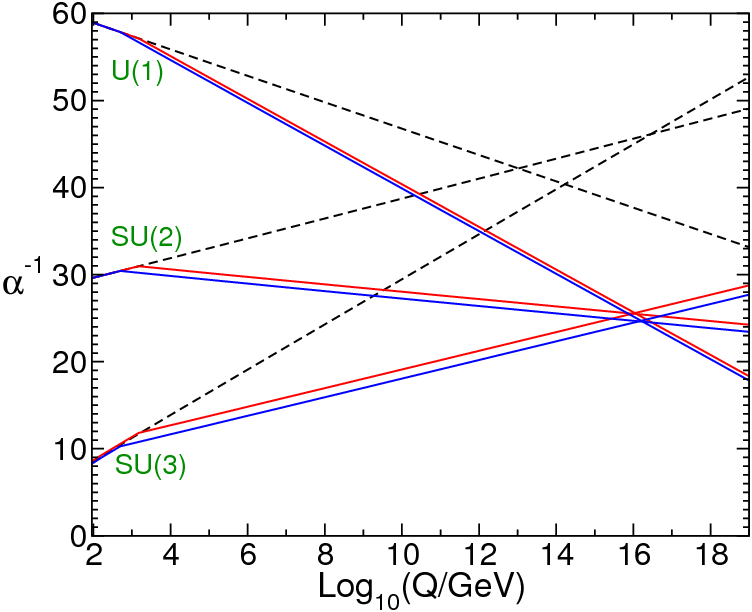
\includegraphics[scale=0.35]{plots/THEO/unification.png}
\caption{Running of the coupling of the electromagnetic, weak and strong force in the Standard Model (dashed lines) and Supersymmetry (red and blue lines).}
\label{fit:unification}
\end{figure}
\section{Supersymmetry}
Of the many proposed extension of the SM, Supersymmetry (SUSY) has been considered to be the most attractive in the last decades. It postulates the existence of a fermion partner to every SM boson and vice versa. This promises a solution to the naturalness problem of the Higgs boson mass and might also lead to a unification of forces and in certain models offer candidates for the dark matter particle. In the following a short description of the theoretical framework, based on~\cite{Martin:1997ns}, is given before the phenomenological consequences and the experimental signatures relevant to this analysis are discussed.
\subsection{Theoretical foundation}
Supersymmetry introduces a symmetry between bosons and fermions. In the minimal supersymmetric extension of the Standard Model (MSSM), one $\textit{superpartner}$ is assigned to each SM particle which has the same quantum numbers except for the spin, which differs by $\frac{1}{2}$. The designated names of the new supersymmetric particles ($\textit{sparticles}$) are derived by adding the prefix $\textit{s-}$ to all fermion partners and the postfix $\textit{-ino}$ to all boson partners. The same scheme holds also for categories of particles, so that $\textit{sleptons}$ and $\textit{squarks}$ are the partners of leptons and quarks and make up the $\textit{sfermions}$ while the $\textit{gauginos}$ are the partners of the gauge bosons. 

The SM Higgs sector has to extended two complex scalar doublets to give masses to the particles
\begin{eqnarray}
H_1 = \colvec{2}{H_1^0}{H_1^-}, & &  H_2 = \colvec{2}{H_2^0}{H_1^+}.
\end{eqnarray}
Here $H_1$ gives mass to down-type quarks and leptons while $H_2$ gives mass to up-type quarks. To these four Higgs states $\textit{higgsinos}$ are introduced as superpartners. In the spontaneous symmetry breaking eight degrees of freedom appear instead of four because of the presence of the second doublet. Three are used to give mass to the W and Z bosons, leaving five massive bosons. Therefore SUSY results in an extended Higgs sectors with two neutral scalars, $h^0$ and $H^0$, one neutral pseudoscalar $A^0$, and two charged scalars $H^{\pm}$. By convention $h^0$ is the lighter of the two scalars and commonly identified with the observed Higgs boson. 

The higgsinos and gauginos mix two eight mass eigenstates, the charginos $\chi^{\pm}_1$ and $\chi^{\pm}_2$ and the neutralinos $\chi^0_1$,$\chi^0_2$,$\chi^0_3$, and $\chi^0_4$. The additional particle content introduced in the MSSM is summarized in Table~\ref{tab:MSSM}.

\begin{table}
\centering
 \renewcommand{\arraystretch}{1.3}
\caption{Additional particle content of the MSSM.}
\label{tab:MSSM}
\begin{tabular}{c|c|c|c}
particle & gauge eigenstates  & mass eigenstates & spin   \\
\hline
\multicolumn{4}{c}{Standard Model} \\
\hline
Higgs bosons & $H_1^0$, $H_1^{-}$, $H_2^0$, $H_2^+$ & $h^0$, $H^0$, $A^0$, $H^{\pm}$ & 0 \\
\hline
\multicolumn{4}{c}{Supersymmetry} \\
\hline
squarks & $\tilde{q}$ & $\tilde{q}$ & 0 \\
sleptons & $\tilde{l}$ & $\tilde{l}$ & 0 \\
 gluino & $\tilde{g}$ & $\tilde{g}$ & 0 \\
neutralinos & $\tilde{W}^0$, $\tilde{B}^0$, $\tilde{H}_1^0$, $\tilde{H}_2^0$ & $\chi^0_1$,$\chi^0_2$,$\chi^0_3$, $\chi^0_4$ & $\frac{1}{2}$\\
charginos & $\tilde{W}^+$, $\tilde{W}^-$, $\tilde{H}_1^-$, $\tilde{H}_2^+$ & $\chi^{\pm}_1$,$\chi^{\pm}_2$ & $\frac{1}{2}$ \\ 
\end{tabular}
\end{table} 

If such a model would be realized it would alleviate the hierachy problem because the contributions of the superpartners to the quantum loop corrections to the Higgs mass have opposite sign than those of the SM particles, cancelling the dependency on the cutoff parameter $\Lambda_{UV}$. However, as no superpartners have been discovered so far, SUSY must be a broken symmetry and they can't have the same mass as the corresponding SM particles but must be heavier. Therefore the cancellation of contributions to the Higgs boson mass becomes imperfect. To prevent the need for fine-tuning, sparticle masses are expected to be at the TeV scale. Especially the top squark mass must to rather small as the top quark is the heaviest SM particle and contributes dominantly to the loop corrections. 

SUSY introduces lepton- and baryonnumber violating couplings, which would allow for rapid proton decay, in contradiction to its extremely long lifetime. To keep the proton stable, the quantum number R-parity
\begin{equation}
R_P = (-1)^{3(B-L)+2s}
\end{equation} 
is introduced, with B, L and s being the baryon number, lepton number and spin of the particle. It is +1 for all SM particles and -1 for all SUSY particles. If R-parity is conserved, SUSY particles can only produced in even number and the lightest supersymmetric particle (LSP) must be stable. In many SUSY models the LSP is the lightest neutralino $\chi^0_1$, providing a possible dark matter candidate. 


\subsection{Dilepton mass edges in SUSY}
The multitude of superpartners offer a rich variety of experimental to be observed at hadron colliders such as the LHC. The discussion here focusses on R-parity conserving models. In Figure~\ref{fig:SUSYXSecs}, the pair production cross section for different combinations of SUSY particles in proton-proton collision at a centre-of-mass energy of $\unit{\sqrt{s}=8}{\tera\electronvolt}$ is shown. It can be seen that the production of squarks and/or gluinos via the strong force is the dominant production mode. It therefore seems natural to focus on these events in the search for SUSY.
\begin{figure}
\centering
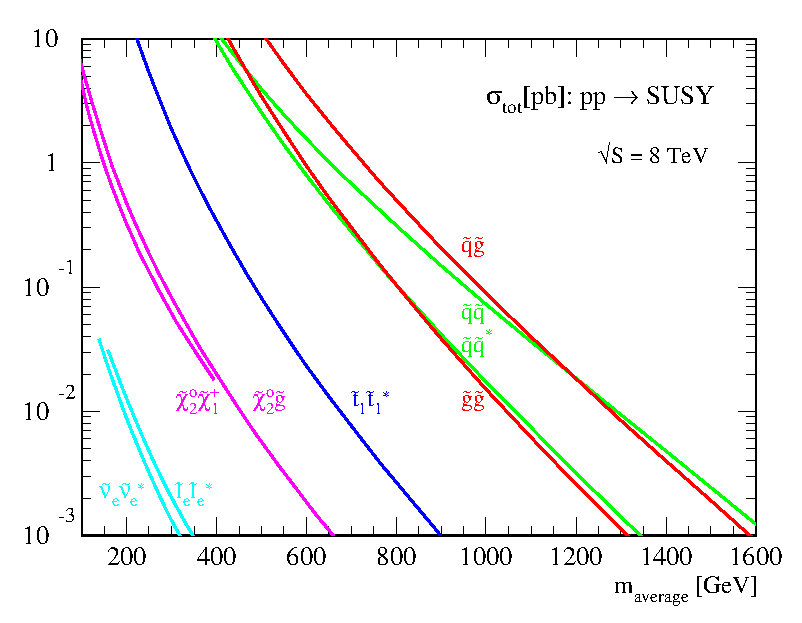
\includegraphics[scale=0.6]{plots/THEO/prospino_lhc8.eps}
\caption{Cross sections for pair production of SUSY particles in proton-proton collision at $\sqrt{s} = \unit{8}{\tera\electronvolt}$ as a function of the average mass of the produced pair~\cite{ProspinoPlot,Beenakker:1999xh,Beenakker:1997ut,bib-nlo-nll-01}.}
\label{fig:SUSYXSecs}
\end{figure}

The experimental signature of SUSY are cascades of decays of the initially produced particles into the LSP under emission of several SM particles. In the case of strong production, at least two quarks or gluons are produced in the first decays of the two decay chains in the events. These will hadronize into jets. Often even more jets are produced in the decays chains, making high jet multiplicities and large amounts of hadronic energy typical signatures of SUSY. The LSP is stable and will leave the detector undetected, adding missing energy to the signature.

As leptons are easy to identify and can be measured precisely, requiring the presence of leptons in the events helps to suppress backgrounds from SM processes such as QCD multijet production. Of particular interest to this analysis are SUSY cascades in which contain the correlated production of lepton pairs of the same flavour but opposite electric charge. Due to their more challenging experimental signature, $\tau$ leptons are not considered. The relevant decay is that of a next-to-lightest neutralino into the lightest neutralino and two leptons $\secondchi \rightarrow \firstchi \ell^+\ell^-$, which can occur either via an intermediate slepton or an off- or on-shell Z boson:
\begin{align}
\secondchi &\rightarrow \tilde{\ell}^{\pm}\ell^{\mp} \rightarrow \ell^{\pm}\ell{\mp}\firstchi,\label{eq:slepton}\\ 
\secondchi &\rightarrow \mathrm{Z}^{(*)}\firstchi \rightarrow \ell^+\ell^-\firstchi.\label{eq:Z}
\end{align}
The decays are illustrated in Figure~\ref{fig:edgeFeyn}, where the left graph corresponds to equation~\ref{eq:slepton} and the right to equation~\ref{eq:Z}.
\begin{figure}[htbp]
\centering
\begin{minipage}[t]{0.49\textwidth}
  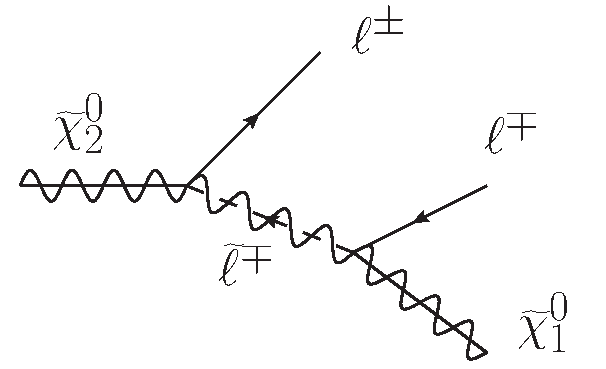
\includegraphics[width=\textwidth]{plots/THEO/FeynmanGraph_slepton.pdf}
\end{minipage}
\begin{minipage}[t]{0.49\textwidth}
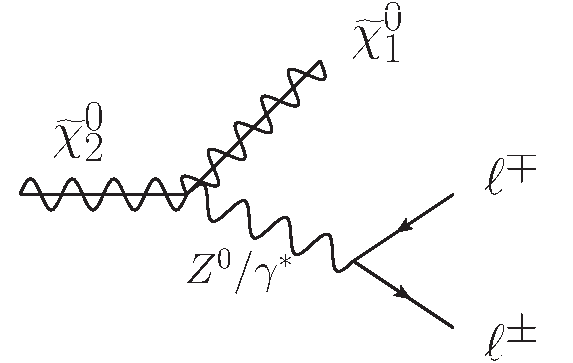
\includegraphics[width=\textwidth]{plots/THEO/FeynmanGraph_Z_decay.pdf}
\end{minipage}
\caption{Graphs for the decays of \secondchi into $\firstchi\ell^+\ell^-$ via an intermediate slepton (left) and off- or on-shell Z boson. Graphs by Christian Schomakers.}
\label{fig:edgeFeyn}
\end{figure}

The mass difference between the two neutralinos sets an upper bound on the invariant mass of the dilepton system \mll and its distribution exhibits an characteristic edge structure. The endpoint of this edge is defined by the signal kinematics.  If the \secondchi decays via an off-shell Z boson, it is simply given by the mass difference itself:
\begin{equation}
\mlledge = m_{\secondchi} - m_{\firstchi}.
\end{equation}
If the decay is mediated via a slepton, this is modified by the slepton mass $m_{\tilde{\ell}}$
\begin{equation}
\mlledge = \sqrt{\frac{(m_{\secondchi}^2-m_{\tilde{\ell}}^2)(m_{\tilde{\ell}}^2-m_{\firstchi}^2)}{m_{\tilde{\ell}}^2}}. 
\end{equation}
For decays via and on-shell Z boson, \mll will be consistent with the Z boson mass and no edge structure is present. The exact shape of the edge is also determined by the decays. For intermediate Z bosons, it will be peaked towards the Z boson peak for \mlledge below the Z peak. For \mlledge on and above the Z boson peak, the decays via and on-shell Z boson dominate and there is no edge. Decays via an intermediate sleptons lead to triangular edge shapes, but the actual shape depends on model parameters, as for example negative interference between the decay channels via slepton and Z boson can occur. Examples are given in the next section.
\subsubsection{Simplified models}
\label{sec:models}
As benchmark scenarios for these signatures, two ``simplified models'' are used that have been developed for this purpose by Christian Schomakers in the context of his master thesis~\cite{Schomakers:2014zza}. In this kind of models, only the subset of sparticles relevant to the studied signature is assumed to be accessible at LHC energies. Also, the branching fractions of the sparticle decays are chosen to produce the desired signature and are often set to 100\%.  

Both models consider the pair production of bottom squarks. They decay into a bottom quark and a \secondchi with a branching fraction of 100\%. The decays of the \secondchi differ between the two models. The Feynman graphs of both models are shown in Figure~\ref{fig:sigFeyn}.

\begin{figure}[htbp]
\centering
\begin{minipage}[t]{0.49\textwidth}
  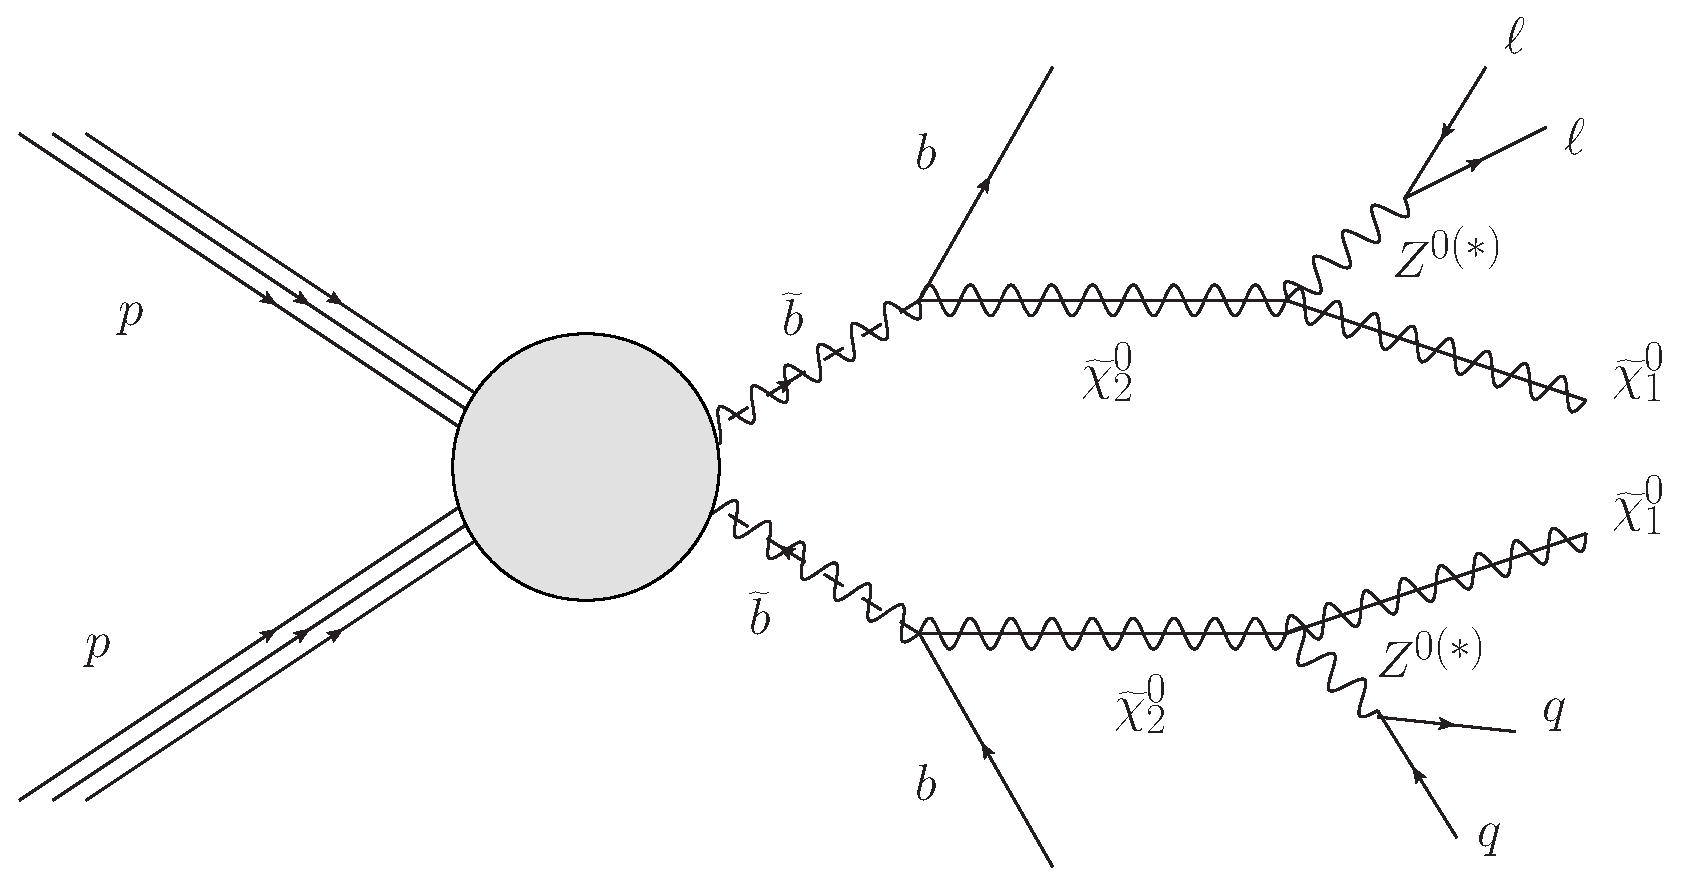
\includegraphics[width=\textwidth]{plots/THEO/Feynman_graph_T6bblledge.pdf}
\end{minipage}
\begin{minipage}[t]{0.49\textwidth}
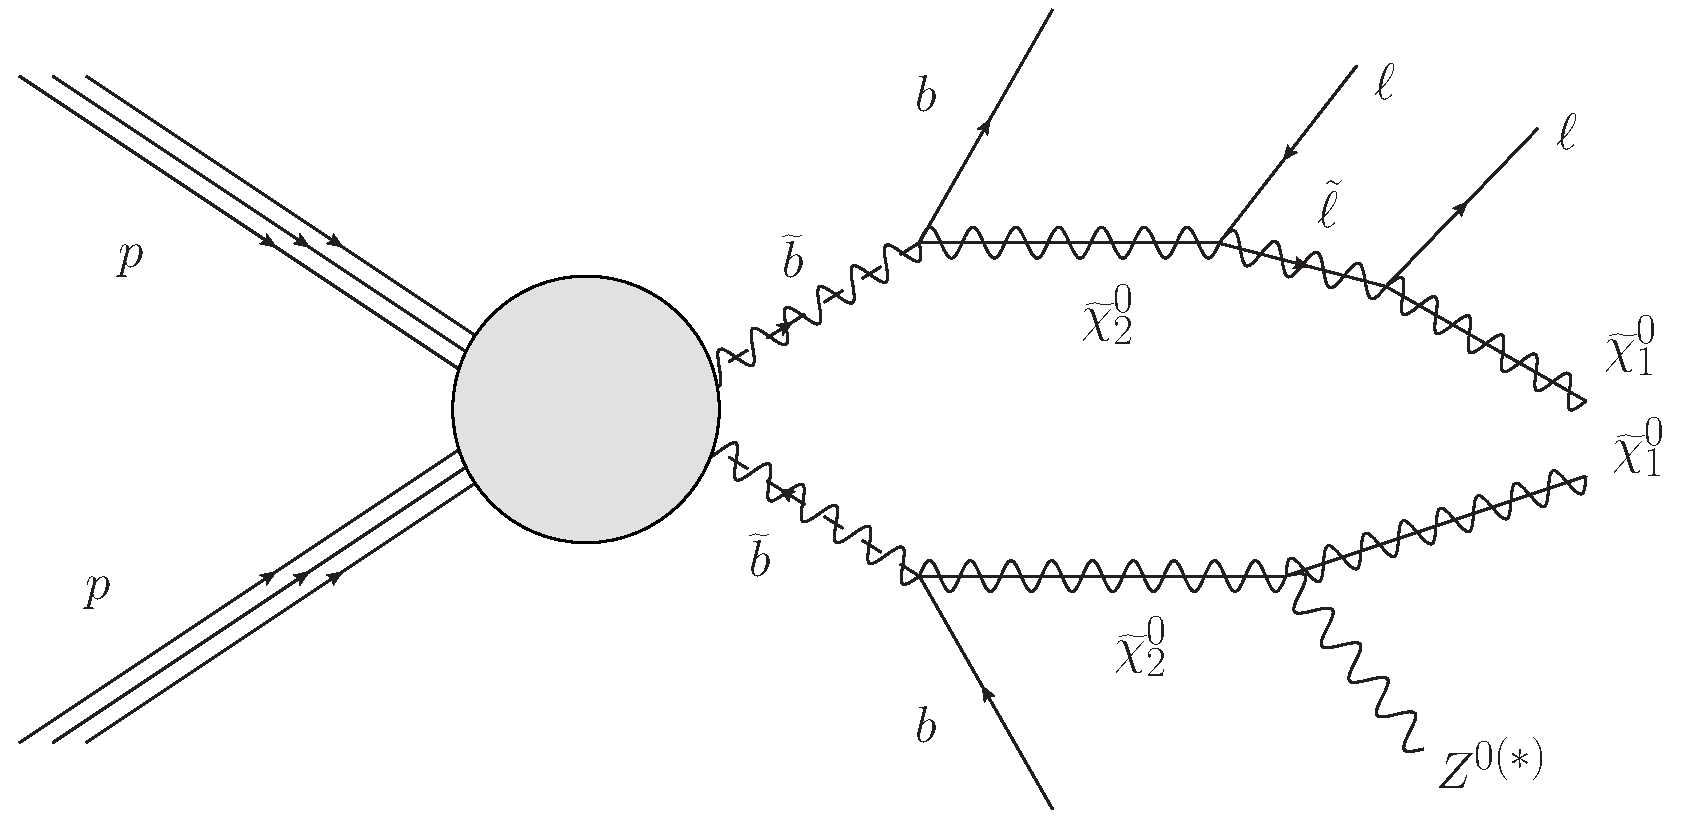
\includegraphics[width=\textwidth]{plots/THEO/Feynman_graph_T6bbslepton.pdf}
\end{minipage}
\caption{Feynman graphs for the fixed-edge (left) and slepton-edge (right) model~\cite{Khachatryan:2015lwa}.}
\label{fig:sigFeyn}
\end{figure}

 In the ``fixed-edge'' model, it decays into an off-shell Z boson and a \firstchi in 100\% of the cases. The Z boson decays with its SM branching ratios, producing light leptons in about 7\% of the cases. The $m_{\sbottom}$-$m_{\secondchi}$-plane is scanned, varying the masses of the two particles in steps of 25\GeV. The mass of the \firstchi is fixed to be 70\GeV below that of the \secondchi to produce an edge in the \mll spectrum at this value.

As a mass difference between the two neutralinos larger than the Z boson mass would only result in the production of on-shell Z bosons in this model, the ``slepton-edge'' model introduces selectrons and smuons as additional new particles. The mass of these sleptons is assumed to be degenerate and set to lie halfway between the two neutralinos: $m_{\slepton} = m_{\firstchi} + 0.5(m_{\secondchi}-m_{\firstchi})$. The branching fractions of the \secondchi are chosen such that the decay in an off- or on-shell Z boson or a slepton and a lepton occur with 50\% probability each. The Z boson again decays according to its SM branching fraction while the slepton always decays into a lepton and the \firstchi. Again the $m_{\sbottom}$-$m_{\secondchi}$-plane is scanned in steps of 25\GeV, while the $m_{\firstchi}$ is set to be 100\GeV, allowing for edges in the \mll spectrum also above the Z boson mass. 
The signal simulation is normalized to theory cross sections calculated at NLO in $\alpha_s$, including the leading logarithmic contributions of the next higher order~\cite{bib-nlo-nll-01,bib-nlo-nll-02,bib-nlo-nll-03,bib-nlo-nll-04,bib-nlo-nll-05,ref:xsec}.

Figure~\ref{fig:SUSYMasses} illustrates the \mll distributions for three example points. The two examples from the slepton-edge model are roughly triangular in shape while the one from the fixed-edge model is peaked toward the Z boson peak as in this model the decay is mediated by an off-shell Z boson. Contributions outside of the edges are caused by events with more than two leptons where the wrong combination has been chosen. In addition to the generated distribution the one reconstructed by a simulation of the CMS detector is shown, illustrating the good detector resolution for lepton pairs.
\begin{figure}
\centering
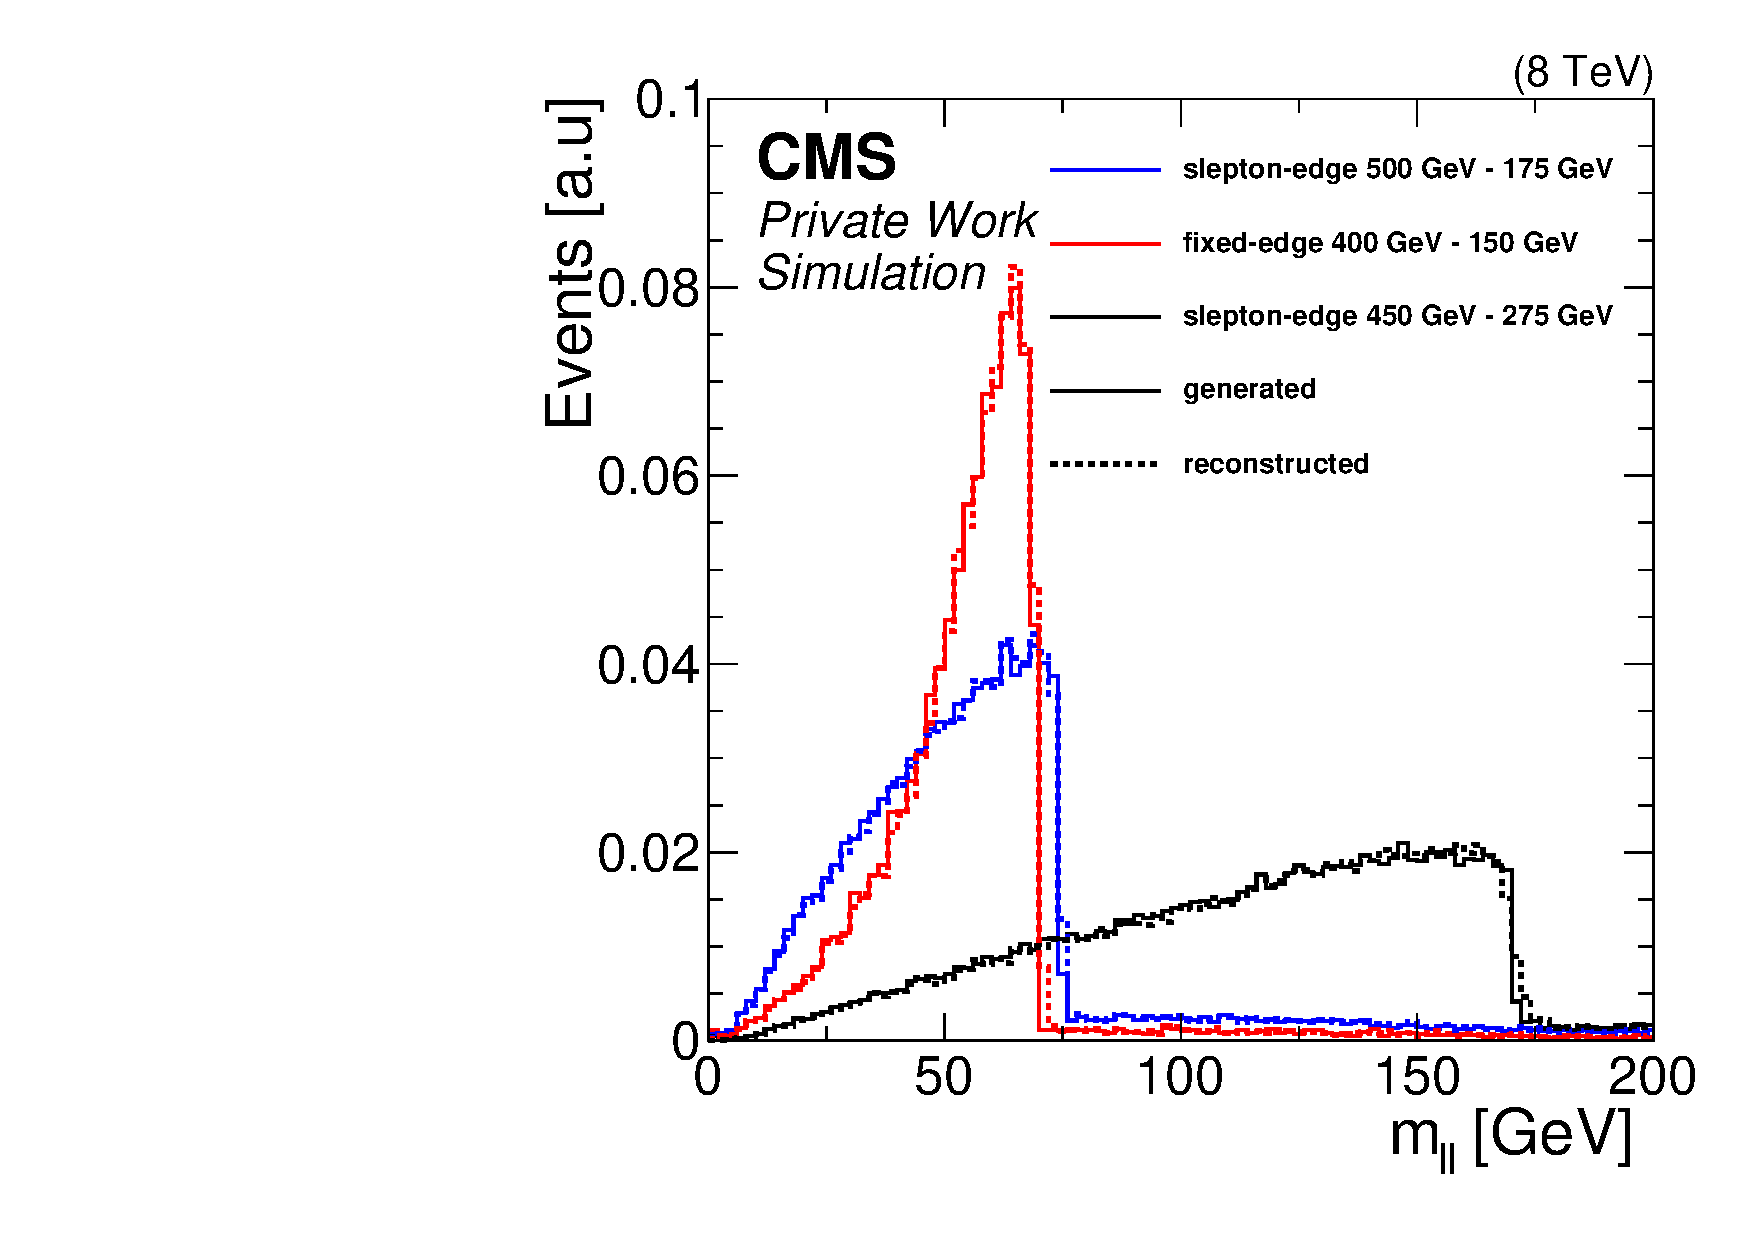
\includegraphics[scale=0.3]{plots/THEO/SUSY_masses.pdf}
\caption{Distribution of \mll for one signal point of the fixed-edge model and two of the slepton-edge model, illustrating different edge positions and shapes. The masses given are those of the \sbottom and \secondchi, respectively. Shown are the generated distributions as solid lines and the reconstructed ones as dashed lines.}
\label{fig:SUSYMasses}
\end{figure}

     
\chapter{Experimental setup}
\section{The CERN Large Hadron Collider}
\section{The CMS detector}
\section{Data acquisition and event reconstruction}
%\chapter{Data triggering and processing}
%\input{Trigger}
%\chapter{Event reconstruction}
%\input{RECO}
%\input{MET}

%\chapter{Dilepton final states in supersymmetric models}
%\input{dileptons}
\chapter{Data analysis and event selection}
\label{sec:ana}
The data recorded by the CMS experiment is processed using dedicated software that uses the detector signals to reconstruct the particles produced in the proton-proton collisions and other properties describing the events. The resulting datasets, accompanied by simulation for both SM and new physics processes, are then analysed. Events are selected using their reconstructed properties based on the characteristics of the physics processes of interest. Here, an overview on the reconstruction algorithms and software is given. Also, the datasets and event selections used in this analysis are motivated.
\section{Object reconstruction}
\label{sec:objects}
The observables most relevant to this analysis are electrons, muons, jets, and the missing transverse energy (\MET). Here, the reconstruction of these objects from the information provided by the CMS detector as performed on the data recorded in 2012 is described. While the electron and muon candidates used in this study are reconstructed independent of each other with dedicated algorithms, jets and \MET are provided by the particle flow (PF) algorithm~\cite{CMS-PAS-PFT-09-001}. It combines information from all subdetectors to achieve a consistent description of the full event. 

\subsection{Vertex reconstruction}
Interaction vertices are reconstructed from the tracks of the charged particles that originate from them.
Tracks fulfilling certain quality requirements are clustered into vertices with a deterministic annealing algorithm~\cite{DertermisiticAnnealing,Chatrchyan:2014fea}. The vertex position is fitted using an adaptive vertex fitter~\cite{Fruehwirth:1027031}, where a weight $w_i$ between 0 and 1 is assigned to every track, based on the likelihood of that track being correctly associated with the vertex. These weights are used to asses the quality of the vertex reconstruction. The vertex with the largest $p_\mathrm{T}^2$ sum of associated tracks is considered to be the primary vertex in the event.

\subsection{Muon reconstruction and identification}
The track of a muon is reconstructed separately in the inner tracker and in the muon system, resulting in a $\textit{tracker track}$ and a $\textit{standalone muon}$. 

Tracks in the inner tracker are reconstructed using a method called combinatorial track finder~\cite{Chatrchyan:2014fea}, which performs pattern recognition and track fitting by employing a Kalman filter technique~\cite{Fruhwirth1987444}. The track is described by a five-dimensional state vector, whose initial parameters are taken from track seeds, determined from three hits or two hits and a vertex constraint in the pixel detector or the innermost layers of the strip detector. The state vector is extrapolated to the next tracker layer taking into account uncertainties and energy losses due to interactions with the tracker material. If tracker hits are found in the modules where they are expected from the extrapolation, they are added to the track candidate. If no hits are found, a ghost hit is added to the track to account for inefficiencies in the hit reconstruction. Too many ghost hits will terminate the reconstruction of the given track. A track fit is then performed to all hits associated with the track candidate, using again Kalman filtering and smoothing. This procedure is performed iteratively, each time removing the hits already associated to a track candidate and relaxing the requirements on the track seeds to allow for reconstruction of tracks with low \pt or not originating from the primary interaction~\cite{SWGuideIterativeTracking}. 

For the reconstruction of $\textit{standalone muons}$ in the muon system, the hits inside the individual muon chambers are fitted to generate track segments, providing first estimates of the track parameters under the hypothesis that the muon was created in the interaction region and was travelling through the muon system from the inside out. These segments are used as starting points for a track reconstruction using all hits from the DTs, CSCs, and RPCs, again using the Kalman filtering technique~\cite{1748-0221-5-03-T03022}.

Tracker tracks are promoted to $\textit{tracker muons}$ when they can be matched to a track segment in the muon detector. $\textit{Standalone muons}$ are matched to tracks from the inner tracker. If a compatible track is found, a combined fit to all hits of the track and the $\textit{standalone muon}$ is performed, resulting in a $\textit{global muon}$. The PF algorithm applies further selection requirements to the reconstructed $\textit{global}$ and $\textit{track muons}$, introducing a fourth category, the $\textit{particle flow muon}$~\cite{CMS-PAS-PFT-10-003}. 

Muons selected in this analysis are required to be reconstructed as $\textit{tracker}$, $\textit{global}$, and $\textit{particle flow}$ muons. The $\chi^2$ per degrees of freedom of the track fit must not exceed 10. Several requirements on the information available for the different track fits are made: At least one muon chamber hit must be included in the track fit of the $\textit{global muon}$. For the fit of the $\textit{tracker muon}$ at least one hit in the pixel detector and six layers with hits in the strip detector have to be available. Also, the track from the inner tracker has to be matched to at least two track segments in the muon chambers. To ensure that the muon originates from the primary interaction and to suppress backgrounds from cosmic muons the impact parameter of the track with respect to the primary vertex must not exceed $\unit{0.02}{\centi\meter}$ in the $x$-$y$ plane and $\unit{0.1}{\centi\meter}$ in $z$ direction. Selected are muons with a \pt larger than $\unit{10}{\giga\electronvolt}$ and $|\eta|$ less than 2.4. The muon selection is summarised in Table~\ref{tab:muonID}.
\begin{table}
\begin{center}
\begin{tabular}{c|c}
Criterion & Selection \\
\hline \hline 
\multicolumn{2}{c}{Acceptance} \\
\hline
\pt & $> \unit{10}{\giga\electronvolt}$ \\
$|\eta|$ & $< 2.4$ \\
\hline
\multicolumn{2}{c}{Muon ID} \\
\hline
Required to be a & $\textit{tracker muon}$ \\
 & $\textit{global muon}$ \\
 & $\textit{particle flow muon}$ \\
 \hline
 \multicolumn{2}{c}{Track quality} \\
 \hline
  $\chi^2/N_{dof}$ & $< 10 $ \\
  valid muon hits & $> 0 $ \\
  matched stations & $> 1 $ \\
  valid pixel hits & $ > 0 $ \\
  tracker layers with hits & $ > 5 $ \\
\hline
  \multicolumn{2}{c}{Impact parameter} \\
\hline
	$d_0 = \sqrt{dx^2 + dy^2}$ & $< \unit{0.02}{\centi\meter}$ \\
	$dz$ & $ < \unit{0.1}{\centi\meter}$ \\  
\end{tabular}
\caption{Summary of the muon selection requirements.}
\label{tab:muonID}
\end{center}

\end{table}
\subsection{Electron reconstruction and identification}
The signature of an electron in the CMS detector is a track reconstructed by the tracking detectors that leads to a matching cluster of energy reconstructed in the ECAL. In practice the reconstruction is complicated by the large material budget of the tracking detectors, resulting in a high probability of an electron to loose energy in form of bremsstrahlung. About 35\% of all electrons loose more than 70\% of their energy and for 10\% the energy loss exceeds 95\%~\cite{Baffioni:2006cd}. The reconstruction has to take into account the large solenoidal magnetic field, which bends the electron's trajectory away from the radiated photons, leading to a spread of the energy in $\phi$~direction. This has to be considered both in the tracking algorithms and in the clustering of the energy deposits in the ECAL. 

In the ECAL barrel and endcaps, two different algorithms are used to group the energy deposits into clusters and clusters of clusters, called super clusters (SCs). Both are designed to group together the energy deposits of the electron itself and those of the bremsstrahlung photons. In the pseudorapidity range of $1.6 < |\eta| < 2.6$ the preshower is located in front of the ECAL and electrons will deposit a fraction of their energy there. The energy deposited in the strips of the preshower between a SC in the ECAL and the primary vertex is summed and added to the energy of this SC~\cite{Anderson:1365024}. 

Electron candidate tracks are refitted with a Gaussian sum filter (GSF) algorithm~\cite{FruhwirtGSFCMS}, which takes into account the energy losses caused by bremsstrahlung. GSF tracking is initiated in two ways. $\textit{ECAL driven seeding}$ requires the presence of a track seed that matches the position of a SC when extrapolating backwards from the ECAL to the tracker~\cite{Baffioni:2006cd}. Alternatively, $\textit{tracker driven seeding}$ is started by tracks fitted with the Kalman filter technique discussed above, that either match the position of ECAL clusters when extrapolated to the ECAL surface, covering the case of no bremsstrahlung, or are of poor quality with only few associated tracker hits~\cite{Chatrchyan:2014fea}. The GSF track and the energy measurement in the ECAL are combined into the final electron candidate. 

The energy losses in the tracker material also impede the determination of the electron charge, as the presence of photon conversions and changes in the trajectory due to radiation can lead to charge misidentififaction when only the GSF track is considered. Therefore, also the associated tracks from the Kalman filter tracking and the supercluster position are used to improve the charge identification~\cite{Khachatryan:2015hwa}.

Electrons are selected requiring \pt larger than $\unit{10}{\giga\electronvolt}$ and $|\eta| < 2.5$. The transition region between ECAL barrel and endcaps of $1.442 < |\eta| < 1.566$ is exluded. To suppress background from muons that radiate photons, electrons with a distance to the nearest $\textit{global}$ or $\textit{tracker muon}$ of less than $\Delta R = 0.1$ are rejected. Backgrounds from for example photon conversions or misidentified charged hadrons are suppressed by a set of selection criteria. The matching of track and supercluster is quantified by the differences between the supercluster position and the parameters of the track extrapolated from the vertex to the ECAL surface in $\Delta\phi$ and $\Delta\eta$. As the energy of the electron is contained in the ECAL, the ratio $H/E$ of hadronic energy deposited in the HCAL behind the electron candidate compared to the energy in the ECAL must be small. The energy spread in the ECAL due to bremsstrahlung occurs in $\phi$ direction. Therefore, no significant spread of the energy in $\eta$, parametrised as
\begin{eqnarray}
\sigma_{i\eta i\eta}^2 = \frac{\sum\limits_i^{5\times 5} w_i\cdot \left(\eta_i - \bar{\eta}_{5\times 5}\right)^2}{\sum\limits_{i}^{5\times 5} w_i},\\
w_i = \max\left(0,4.7 + ln\left(\frac{E_i}{E_{5 \times 5}}\right)\right),
\end{eqnarray}
is expected, where for $5\times 5$ crystals around the seed crystal, which initiated the clustering, the distance in $\eta$ from the mean $\eta$ of the cluster is summed, weighted by the energy deposit in each crystal. For a well measured electron, there is good agreement between the energy deposited in the ECAL and the track momentum measured in the tracker. Therefore, the value of $\left| \frac{1}{E} - \frac{1}{p}\right|$ must be small. Requirements on the impact parameter of the track with the respect to the vertex are made. To reject electrons originating from converted photons, only one pixel layer with a missing hit is allowed. This suppresses most conversions occurring after the first layer of the pixel detectors. To reject also conversion in this first layer and in the beam pipe, vertex fits for the electron track with neighbouring tracks are performed in order to reconstruct the point of conversion. For a prompt electron, the probability of these fits is low and required to be smaller than $10^{-6}.$ Some of these requirements are already applied on HLT level. In order to select electrons for which the trigger is fully efficient, selections at least as strict are applied at analysis level. The specific requirements are listed in Table~\ref{tab:eleID}, separately for barrel and endcap, where appropriate. 
\begin{table}
\begin{center}
\begin{tabular}{c|c|c|c|c}
Criterion & \multicolumn{2}{c|}{Selection at HLT}  & \multicolumn{2}{c}{Selection at Analysis Level}  \\
 & EB & EE & EB & EE \\
\hline \hline 
\multicolumn{5}{c}{Acceptance} \\
\hline
\pt & \multicolumn{2}{c|}{trigger dependent} &  \multicolumn{2}{c}{$> \unit{10}{\giga\electronvolt}$} \\
$|\eta|$ & \multicolumn{2}{c|}{$< 2.5 $} & \multicolumn{2}{c}{$< 2.5 $, excluding $1.442 < |\eta| < 1.566$}  \\

\hline
\multicolumn{5}{c}{ID variables} \\
\hline
$|\Delta \eta |$ & 0.01 & 0.01 & 0.007 & 0.009  \\
$|\Delta \phi |$ & 0.15 & 0.10 & 0.15 & 0.10  \\
$\sigma_{i\eta i\eta}$ & 0.011 & 0.031 & 0.01 & 0.03  \\
$H/E$ & 0.10 & 0.075 & 0.12 & 0.10 \\ 
$\left|\frac{1}{E} - \frac{1}{p}\right|$ & \multicolumn{2}{c|}{-} & 0.05 & 0.05 \\
\hline
\multicolumn{5}{c}{Conversion rejection} \\
\hline
 missing pixel hits & \multicolumn{2}{c|}{-} & $\leq1$  & $\leq1$ \\
 vertex fit probability & \multicolumn{2}{c|}{-} & $< 10^{-6}$ & $< 10^{-6}$ \\ 
 \hline
  \multicolumn{5}{c}{Impact parameter} \\
\hline
	$d_0 = \sqrt{dx^2 + dy^2}$ & \multicolumn{2}{c|}{-} & $< \unit{0.02}{\centi\meter}$ & $< \unit{0.02}{\centi\meter}$\\
	$dz$ & \multicolumn{2}{c|}{-} & $ < \unit{0.1}{\centi\meter}$ & $ < \unit{0.1}{\centi\meter}$\\  
\end{tabular}
\caption{Summary of requirements of the electron selection.}
\label{tab:eleID}
\end{center}
	
\end{table}
\subsection{Observables reconstructed with particle flow}
\label{sec:PF}
The particle flow (PF) algorithm~\cite{CMS-PAS-PFT-09-001} is designed to combine information from all subdetectors to reconstruct a consistent description of the event, resulting in a list of reconstructed particles. The basic building blocks are PF elements, which are reconstructed in each subdetector separately: Tracks of charged particles in the tracker or muon system and energy clusters in the calorimeters. A linking algorithm then combines elements into blocks based on their geometrical distance, for example by extrapolating a track into the ECAL and HCAL and searching for compatible clusters. Similarly, calorimeter clusters are linked between the preshower, ECAL, and HCAL and tracks from the tracker are associated with those from the muon system. $\textit{Particle candidates}$ are reconstructed from the objects inside each block. Muons are reconstructed first, followed by electrons, for which, similar to the standard algorithm described above, a refit of the track with the GSF algorithm is performed and bremsstrahlung photons are collected in the ECAL. Lastly, calorimeter clusters compatible with a track are identified as charged hadrons, while clusters without a matching track are either categorised as neutral hadrons, or, depending on the energy deposits in the HCAL, as photons. 
\subsubsection{Jets}
The particles produced in the hadronisation of quarks and gluons are grouped into jets by clustering algorithms. An anti-$k_T$ algorithm~\cite{Cacciari:2008gp}, performed using a fast implementation~\cite{Cacciari:2011ma,Cacciari:2005hq}, is used in this analysis.  Input to the clustering are the $\textit{particle candidates}$ reconstructed by the particle flow algorithm.

The anti-$k_T$ algorithm is a sequential clustering algorithm. Two distance measures are introduced, the first between two particles or pseudo-jets $i$ and $j$ and the second between particle or pseudo-jet $i$ and the beam axis: 
\begin{equation}
d_{ij} = \min(k_{Ti}^{-2},k_{Tj}^{-2})\frac{\Delta^2_{ij}}{R^2},
\end{equation}
\begin{equation}
d_{iB} = k_{Ti}^{-2},
\end{equation}
with $\Delta_{ij}^2 = (y_i-y_j)^2 + (\phi_i - \phi_j)^2$ and $k_{Ti}$, $y_i$, and $\phi_i$ being the transverse momentum, rapidity, and azimuth of a particle. The distances for all entities (particles, pseudo-jets) are calculated. If the smallest is a $d_{ij}$, $i$ and $j$ are combined in a new pseudo-jet. If the smallest distance is the distance to the beam $d_{iB}$, the pseudo-jet is considered a final jet and removed from the list of particles available for clustering. The parameter $R$ governs the size of the resulting jet and is set to 0.5 in this analysis. 

The measured jet momentum $p_{\mu}^{\text{raw}}$ has to be corrected for energy offsets and the non-uniform and non-linear response of the detector. Each component of the jet's four-momentum vector is corrected by a multiplicative factor~\cite{1748-0221-6-11-P11002}
\begin{equation}
p_{\mu}^{cor} = C \cdot p_{\mu}^{\text{raw}}.
\end{equation} 
The correction is applied as a sequence of different factors: 
\begin{equation}
C = C^{L1}_{\text{offset}}(p_{\mathrm{T}}^{\text{raw}})\cdot C^{L2L3}_{\text{MC}}(p_{\mathrm{T}}^{\prime},\eta)\cdot C^{L2\text{Residual}}_{\text{rel}}(\eta) \cdot C^{L3\text{Residual}}_{\text{abs}}(p_{\mathrm{T}}^{\prime\prime}).
\end{equation}
The $L1$ correction, applied to the raw jet, corrects for offsets due to the underlying event and pileup using a jet area approach. The particles in the event are clustered with a $k_T$ jet clustering algorithm~\cite{Catani:1991hj} with a distance parameter $R=0.6$, which clusters a large number of soft jets in each event. The jet area $A_j$ is determined for each of these jets. The median \pt density $\rho$ is then defined as the median of the distribution of $p_{\mathrm{T}_j}/A_j$ for all of these jets. Because of the large number of jets originating from secondary interactions, $\rho$ is not influenced by the presence of hard jets from the primary interaction in the event and is a measure for the pileup activity, the underlying event, and electronic noise. Jets are then corrected by the factor $C^{L1}_{\text{offset}}(p_\mathrm{T}^{\text{raw}}) = 1-\frac{(\rho-\left<\rho_{UE}\right>)\cdot A_j}{p_\mathrm{T}^{\text{raw}}}$, where $\left<\rho_{UE}\right>$ is the mean \pt density due to the underlying event, measured in events with no pileup interactions. $C^{L2L3}_{\text{MC}}$, derived from simulation, corrects for the non-linearities and non-uniformities of the detector response to jets of different $\pt$ and $\eta$ and are applied to the offset-corrected jets. To correct for residuals differences between simulation and data, $C^{L2\text{Residual}}_{\text{rel}}(\eta)$ and $C^{L3\text{Residual}}_{\text{rel}}(p_{\mathrm{T}}^{\prime\prime})$, derived from dijet and Z/$\gamma$+jets data, are applied to jets in data events. 

In this analysis, the \pt of a jet is required to exceed $\unit{40}{\giga\electronvolt}$ and jets are required to lie inside the fiducial volume of the ECAL of $|\eta| < 3.0$. A set of loose quality selections is applied to suppress jets reconstructed because of detector noise, ensuring that the jet is reconstructed in more than one subdetector and has more than one constituent. To prevent an overlap between selected objects, jets within $\Delta R = 0.4$ to leptons identified with the criteria described above are rejected. 

Because of their long lifetime, b-hadrons decay at a measurable distance from their production vertex, allowing for the reconstruction of a secondary vertex. In this analysis the $\textit{combined}$ $\textit{secondary}$ $\textit{vertex}$ (CSV) algorithm is used. Likelihood ratios based on a variety of variables characterizing the secondary vertex and the tracks inside the jet are used to construct a single discriminator. If the value of this discriminator exceeds a given threshold, the jet is tagged as originating from a b-quark~\cite{Chatrchyan:2012jua}. The performance of the b-tagging algorithms have been measured on the dataset recorded at $\sqrt{s} = \unit{8}{\tera\electronvolt}$~\cite{CMS-DP-2013-005}. The average identification efficiency as a function of the discriminator value is shown in Figure~\ref{fig:bTagging} (top). In this analysis, a jet is tagged as a b-jet if the discriminator is larger than 0.679. For this working point the efficiency is about 70\% while the probability to misidentify a jet originating from a light quark as a b-jet is between 1\% and 3\%, depending on the \pt of the jet, as shown in Figure~\ref{fig:bTagging} (bottom). In this analysis b-jets with a \pt larger than $\unit{30}{\giga\electronvolt}$ and $|\eta| < 2.4$ are considered. 
\begin{figure}[htbp]
\centering

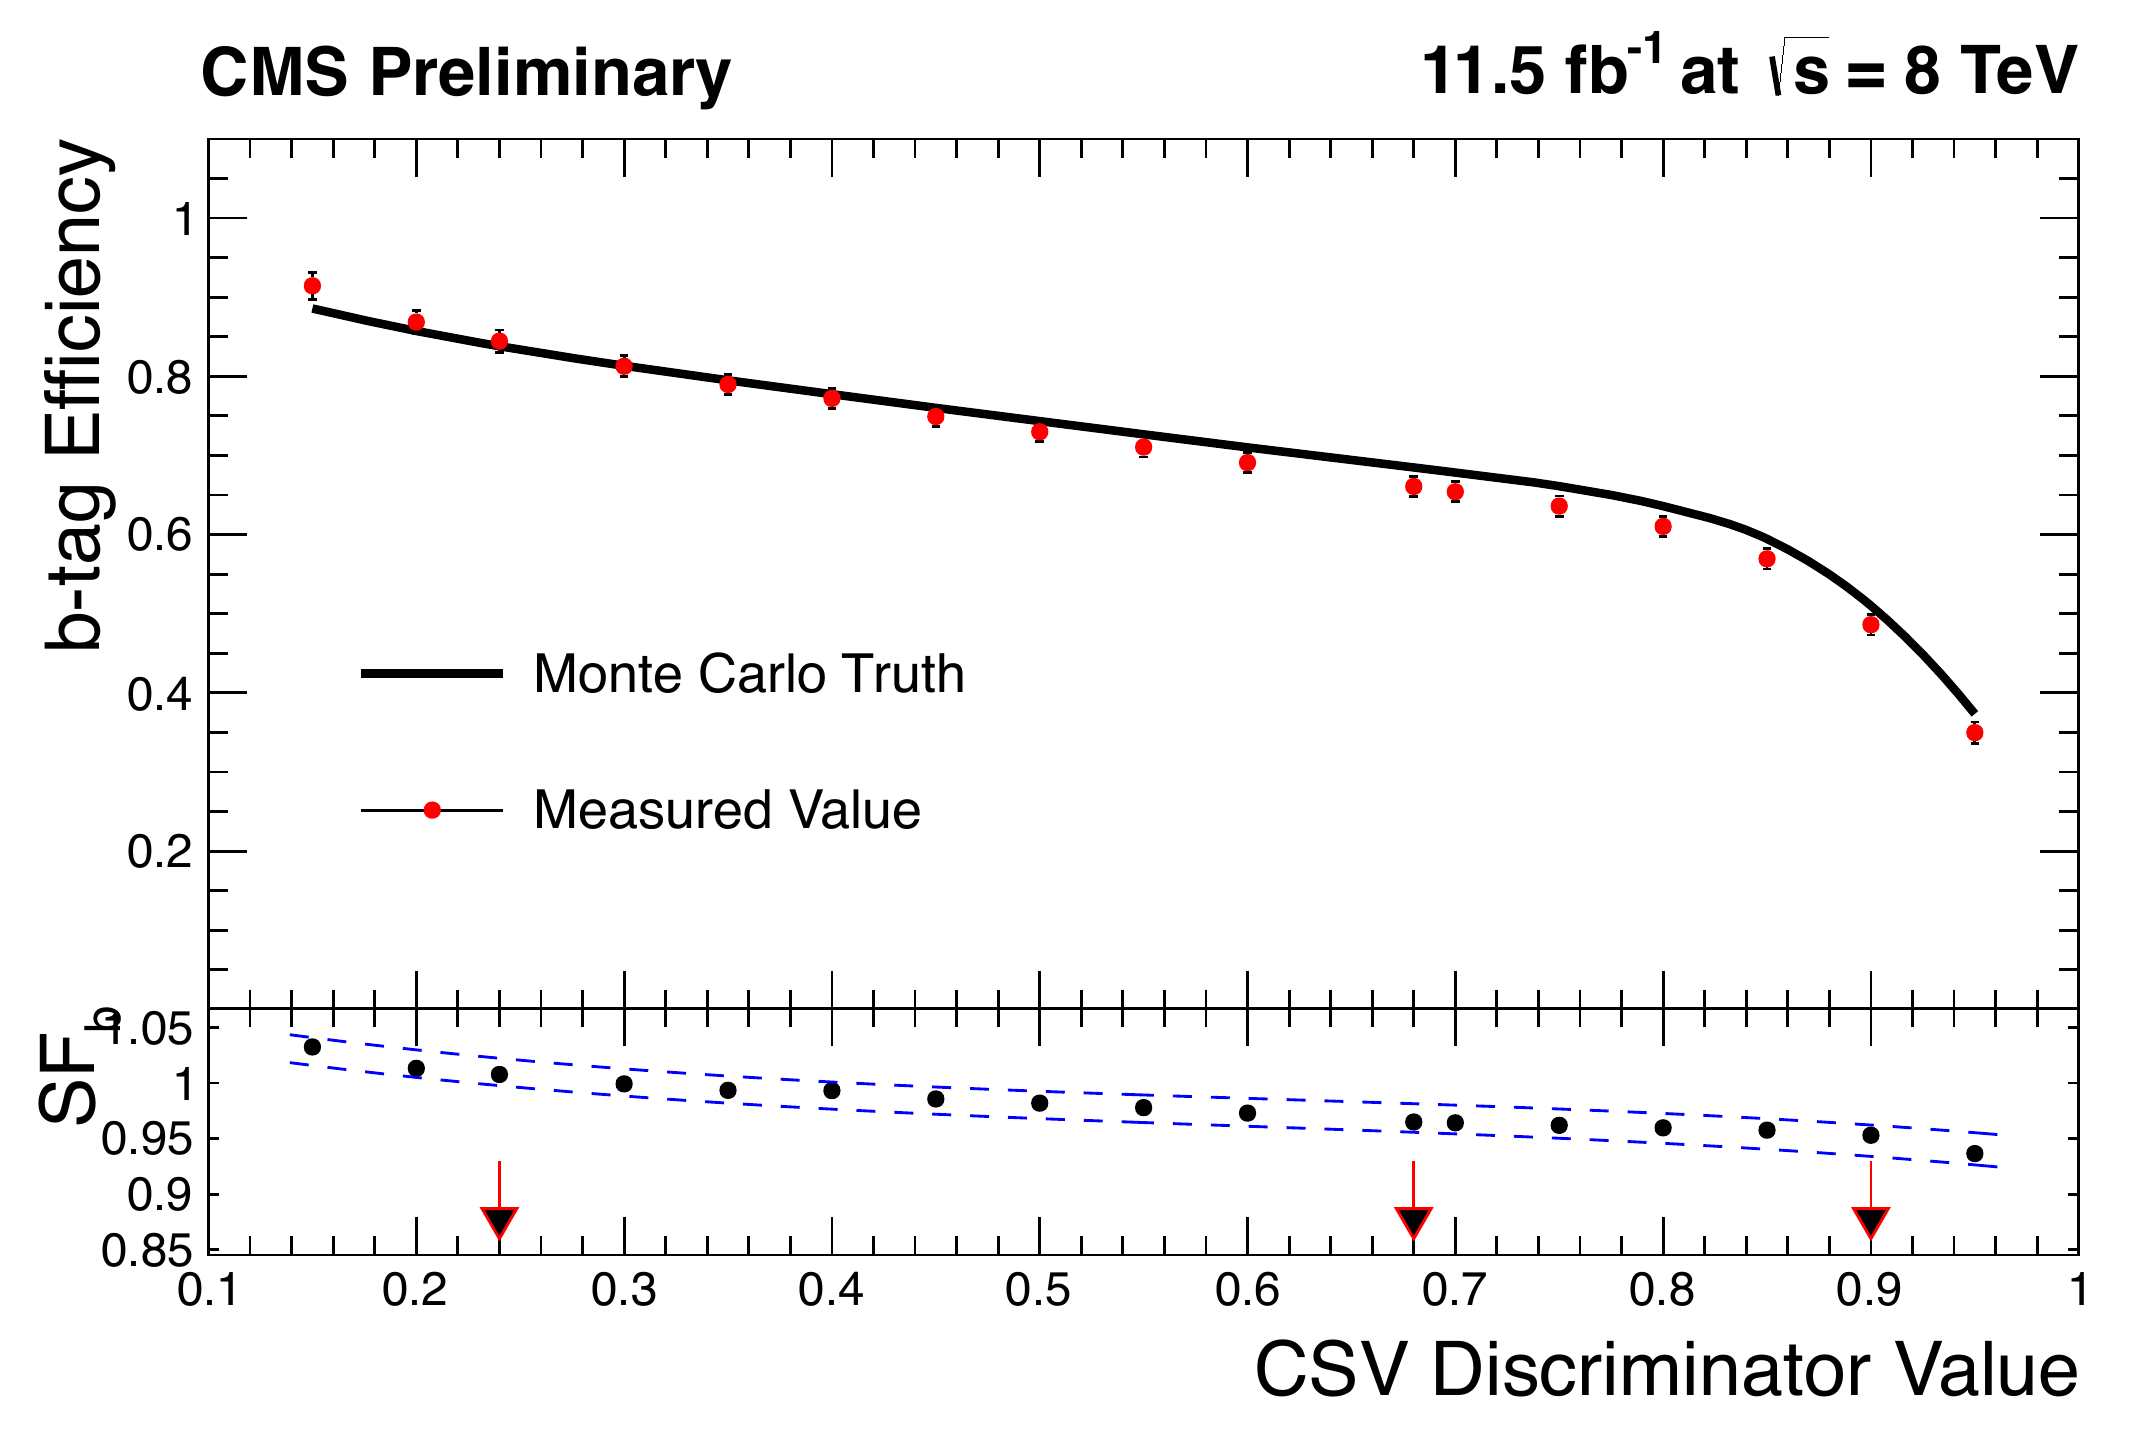
\includegraphics[width=0.6\textwidth]{plots/RECO/bTagEfficiency.png}\\

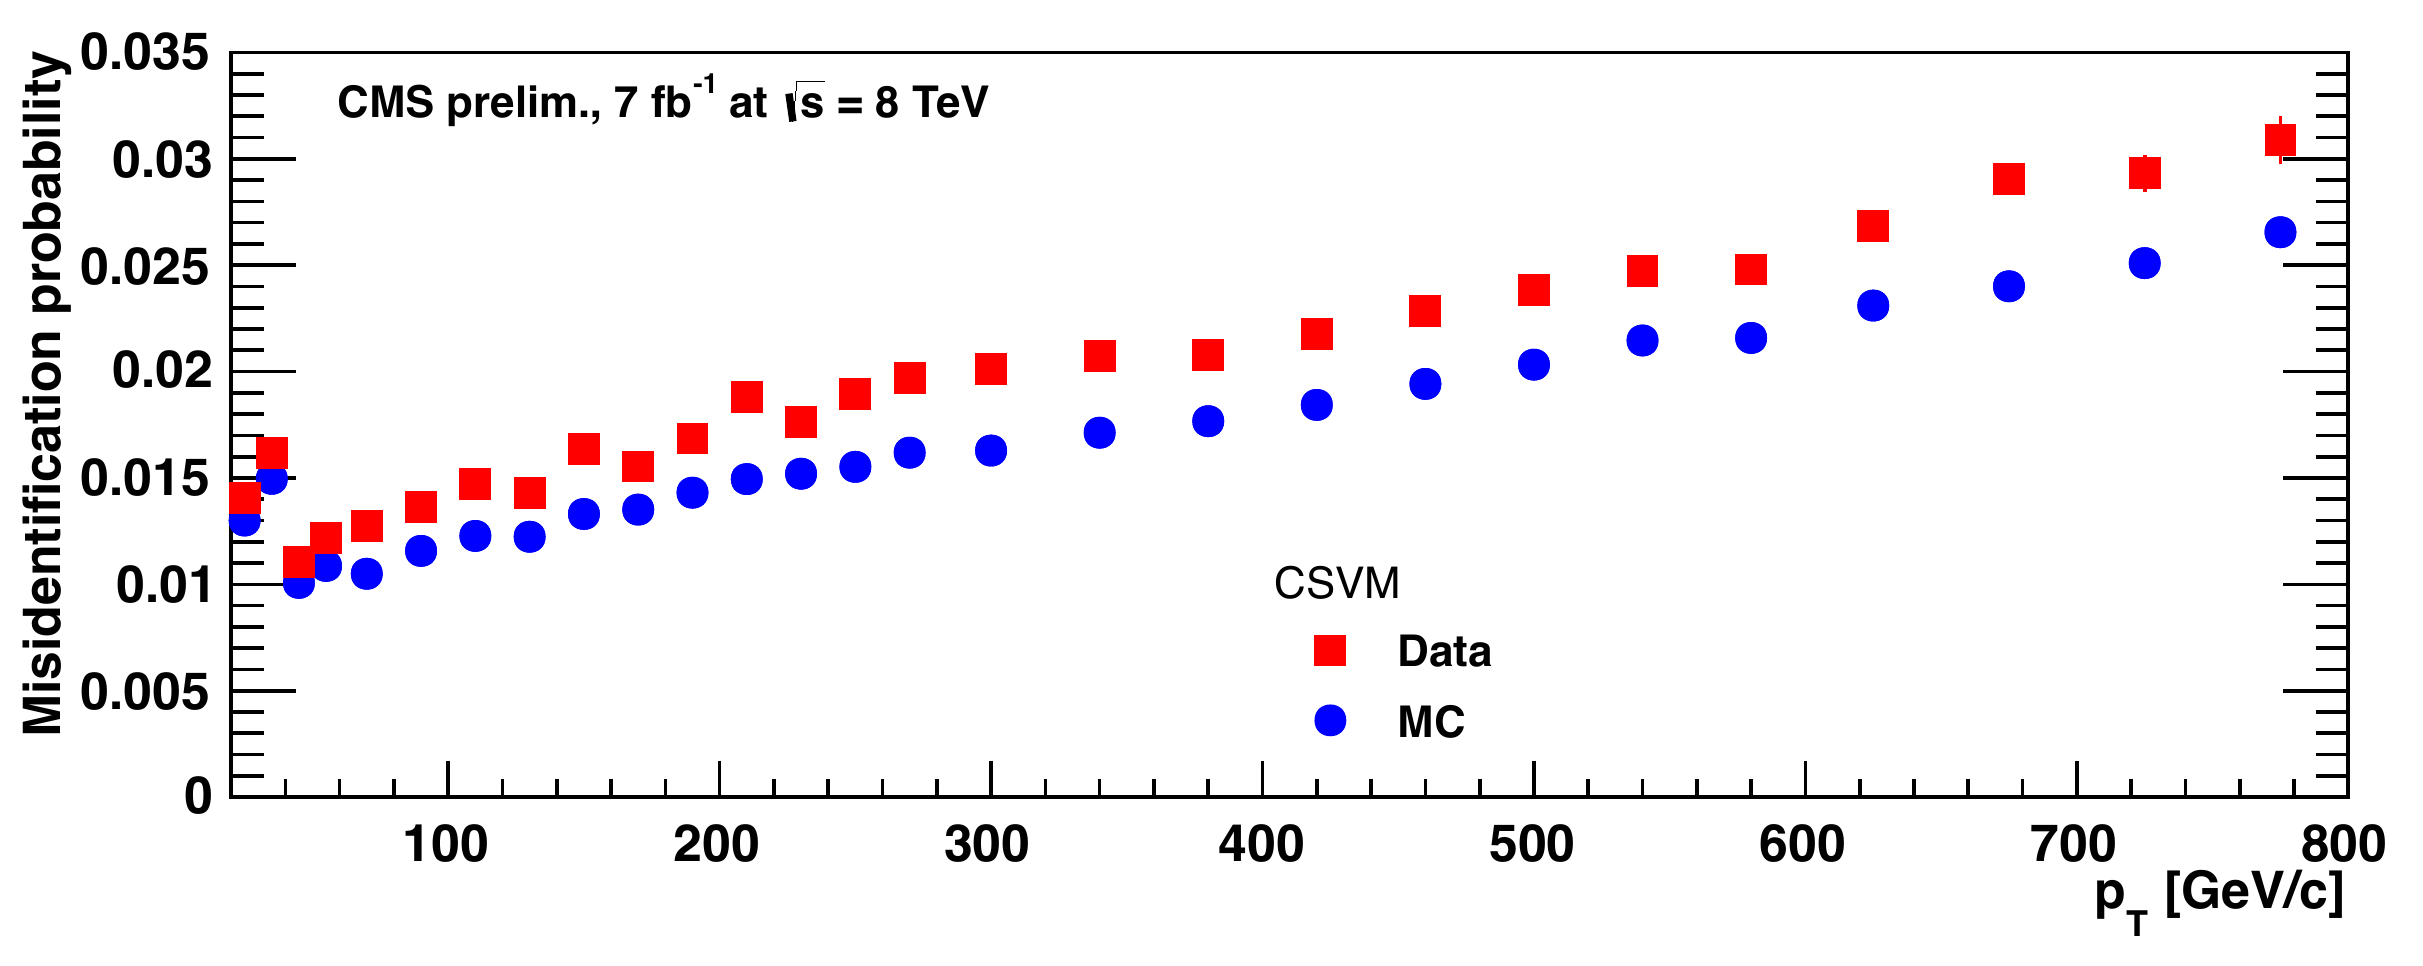
\includegraphics[width=0.6\textwidth]{plots/RECO/bTagMisID.png}\\

\caption{Performance of the CSV b-tagging algorithm. Shown is the identification efficiency as a function of the discriminator value (top) and the probability of misidentifying a jet originating from a light quark as a b-jet for the discriminator value of 0.679 used in this analysis (bottom) as a function of \pt~\cite{CMS-DP-2013-005}. In the top figure, the scale factor between data and simulation is shown below the plot. The red arrows indicate three working points used in CMS.}
\label{fig:bTagging}
\end{figure} 

\subsubsection{Missing transverse energy}
As discussed in Section~\ref{sec:variables}, \MET measures the imbalances of the energy depositions in the detector in the plane transverse to the beam direction. As this imbalance is the only experimental signature of this class of particles, a good \MET resolution is a key factor for the discovery of processes that include the production of new weakly interacting particles. 

Several algorithms have been developed in CMS to reconstruct \MET~\cite{7TeVMETPaper}. Calorimetric (Calo)~\METVec is calculated as the negative vector sum of the energy deposits in each calorimeter tower. Muons deposit only very small amounts of energy in the calorimeters, and are replaced by the measured muon \pt for this calculation.  Track-corrected (TC)~\METVec differs from Calo~\METVec in the treatment of charged hadrons. For well reconstructed tracks, the track measurement is more precise than the measurement of a hadron's energy in the HCAL. Therefore, for tracks not associated with an electron or  muon, the track measurement is used in the calculation of \METVec. The energy deposit in the calorimeter is excluded, based on a model of the calorimeter response, treating all hadrons as pions. In contrast to these subdetector-based approaches, the event description of the particle flow algorithm can be used to calculate \METVec. It is defined as the negative vector sum over the \pt vectors of all \textit{particle candidates}
\begin{equation}
 \METVec = - \sum\limits_{\textit{particle candidates}} \vec{p}_\mathrm{T}.
\end{equation}
Several corrections can be applied to the calculation of \MET. The $\textit{type-I}$ corrections propagate the jet energy corrections  to the \MET calculation for all jets with \pt larger than $\unit{10}{\giga\electronvolt}$ and with less than 90\% of their energy deposited in the ECAL. The effects of pileup on the \MET reconstruction can be mitigated by applying $\textit{type-0}$ corrections, which are calculated on minimum bias events to parametrise the effects of such interactions on \MET. Additionally, $\textit{type-I}$ corrected \MET can be further adjusted using $\textit{type-II}$ corrections that take into account effects caused by the underlying event. Further corrections can be applied to correct for modulations of the \MET in $\phi$~\cite{CMS-PAS-JME-12-002}. As this analysis searches for events with a large genuine \MET and is therefore not very sensitive to \MET introduced by resolution effects, none of these corrections are applied. 

Comparing the resolution for the \MET components in $x$ and $y$ direction, after calibrating for the different response of the algorithms, as shown in Figure~\ref{fig:METReso} for the data collected in 2011, PF \MET performs better than TC and Calo \MET and is therefore used in this analysis. However, the other two, as well as $\textit{type-I}$ corrected PF \MET, are considered as cross-checks. 
\begin{figure}[htb]
\begin{center}
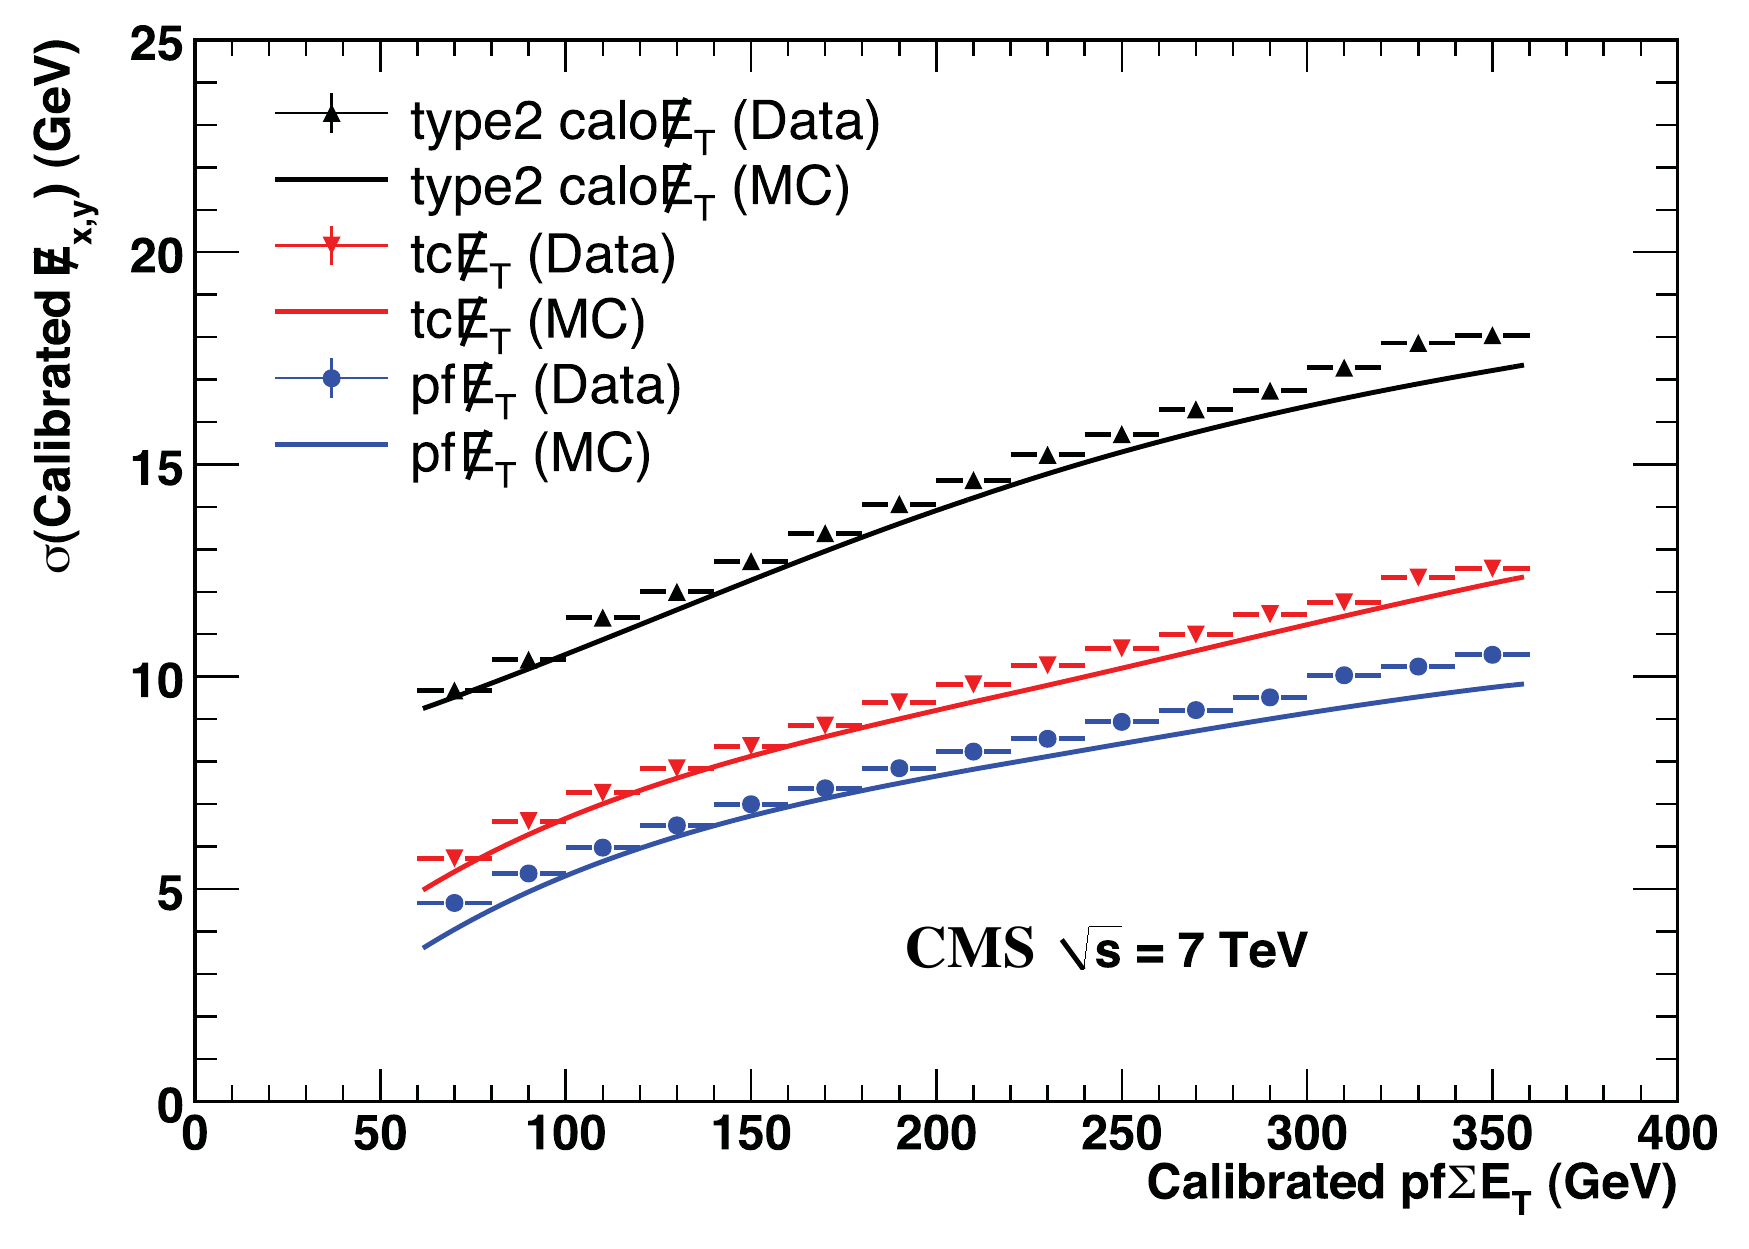
\includegraphics[scale=0.2]{plots/RECO/METResolution.png}
\caption{\MET resolution as a function of the sum of the \Et of all particle flow candidates in an event after calibrating for the different response of the algorithms. Shown are $\textit{type-II}$ corrected Calo \MET as black upward pointing triangles, TC \MET as red downward pointing triangles, and PF \MET as blue points~\cite{7TeVMETPaper}.}
\label{fig:METReso}
\end{center}
\end{figure}


\subsubsection{Lepton isolation}
While the lepton selection criteria described above are sufficient to reject backgrounds from particles misidentified as leptons, they do not suppress real leptons not originating from the primary interaction. As these are often produced in decays of heavy flavour quarks inside a jet, a more suitable criterion is to consider the amount of activity in the detector close to the lepton candidate, called lepton isolation. In this analysis, particle based isolation is used. For this the \pt of charged hadron, neutral hadron, and photon \textit{particle candidates} in a cone of $\Delta R = 0.3$ around the lepton is summed:
\begin{equation}
\text{Iso}^{\text{uncorrected}} = \sum\limits_{\text{charged hadrons}} \pt + \sum\limits_{\text{neutral hadrons}} \pt + \sum\limits_{\text{photons}} \pt.
\end{equation}
The calculation of the isolation is distorted by pileup if PF candidates originating from pileup interactions lie within the cone and are counted in the isolation sum. This is easily remedied for charged hadrons, as those originating from a pileup vertex can be excluded from the calculation. For neutral hadrons and photons there is no track that can be associated to a vertex and a direct identification as pileup particles is not possible. Different approaches are pursued to correct for this contribution for electrons and muons. In both cases, an estimate for the contribution of neutral pileup is subtracted from the isolation sum, which changes the isolation variable to:
\begin{equation}
\text{Iso} = \sum\limits_{\text{charged hadrons from PV}} \pt + \max\left(0, \sum\limits_{\text{neutral hadrons}} \pt + \sum\limits_{\text{photons}} \pt - \sum\limits_{\text{neutral PU}} \pt\right), 
\label{eq:iso}
\end{equation}
where $\sum\limits_{\text{neutral PU}} \pt$ is the estimated pileup contribution from neutral hadrons.
For electrons the correction is similar to the L1 offset correction for jets described above. As a measure of the pileup contribution in the isolation cone the median \pt density in the event $\rho$ is multiplied by the effective area of the electron's isolation cone in the detector, which is calculated in bins of $\eta$. The pileup correction is therefore defined as $\sum\limits_{\text{neutral PU}} E_T = \rho\cdot A^{\text{eff}}_{\text{electron}}$. For muons $\Delta \beta$ corrections are applied. On average, the contribution of neutral particles from pileup is half that of charged particles, leading to a correction defined as $\sum\limits_{\text{neutral PU}} E_T = \Delta\beta\cdot \sum\limits_{\text{charged PU}} E_T$ with $\Delta\beta = 0.5$. Because of the stochastic nature of these approaches, overcorrection is possible. Therefore, no negative contribution from neutral particles is allowed in Equation~\ref{eq:iso}. For both electrons and muons the isolation sum divided by the lepton candidate \pt (relative isolation $\frac{\text{Iso}}{\pt}$) must not exceed  15\%. The choice of this requirement is discussed in more detail in Section~\ref{sec:inclusiveSelection}.

 
\section{Event processing and datasets}
Events accepted by the HLT are reconstructed using the algorithms described above, implemented in the CMS software (CMSSW) framework~\cite{PTDR1,SWGuideCMSSW}. While a first reconstruction is performed immediately after the data is recorded, making it available to analysis within a few days, the full dataset recorded by CMS in 2012 has been reprocessed in a second reconstruction with updated calibrations and detector alignment in the first months of 2013. The software version used for this purpose was ``\verb+CMSSW 5.3.7 patch6+''. The events are stored in the analysis object data (AOD) format, which contains mostly high level objects, such as electrons and muons, and does not provide access to detailed detector information such as energy deposits, which are not of interest for many analyses. This allows to reduce the event size to $\unit{\approx0.1}{\mega\byte}$, compared to about $\unit{2}{\mega\byte}$ for the raw detector output. 

The data processing in this analysis is split into two parts. As a first step, the events in AOD format are processed utilising the resources of the worldwide LHC computing grid~\cite{doi:10.1146/annurev-nucl-102010-130059,WLCG}, a system of cross-linked computing centres providing storage and computing capacities to the LHC experiments.  Datasets stored on grid sites can be accessed through the CMS remote analysis builder~\cite{CRAB}. At this stage, dilepton events are selected based on the identification criteria described above and the properties of the lepton pairs, together with other event characteristics, are stored. This is done with version ``\verb+V00-05-24+'' of the \verb+SuSyAachen+ framework, which utilises tools provided within the CMSSW framework, notably the physics analysis toolkit~\cite{PATNote}. All datasets used in this analysis have been processed using ``\verb+CMSSW 5.3.8 patch3+''. Detector calibrations and alignment constants used in the processing of events in CMSSW are specified in so called \verb+Global Tags+. The tags used in this analysis are ``\verb+FT53_V21A_AN6+'' for data and ``\verb+START53_V27+'' for simulation.

The second part consists of all further analysis performed on the events selected in the previous processing. As the event size is much reduced, it can be performed using conventional desktop PCs. Throughout the event processing chain, the ROOT framework ~\cite{ROOT} for data analysis in particle physics is frequently used. In the final analysis steps, ROOT version \verb+5.34.21+ is used.  

\subsection{Primary datasets}

Events are sorted into different primary datasets based on the HLT decisions, grouping together events accepted by related triggers. As this allows for events to appear in several of theses datasets, precautions against double counting have to taken when combining different data streams in one analysis. The primary datasets most relevant to this analysis are \verb+DoubleElectron+, \verb+DoubleMu+, and \verb+MuEG+, containing, amongst others, events triggered by the different dilepton triggers. As auxiliary datasets, events from primary datasets triggered by \HT (\verb+HT+, \verb+JetHT+), single leptons (\verb+SingleElectron+, \verb+SingleMu+), and $\alpha_\mathrm{T}$ (\verb+HT+, \verb+HTMHT+) are used (see Section~\ref{sec:trigger}). Each primary dataset is split into four subsets, labelled \verb+Run2012A+ to \verb+Run2012D+, each run defined by the run period of the LHC between two technical stops. The primary datasets are summarised in Table~\ref{tab:datasets}, where also the dataset paths by which the samples can be accessed in the CMS bookkeeping system (DBS)~\cite{1742-6596-119-7-072001} is given.   

\begin{table}

\begin{center}
\begin{tabular}{c|c|c}
 Primary dataset & purpose & dataset \\
\hline 
\verb+DoubleElectron+ & Signal & \verb+/DoubleElectron/Run2012A-22Jan2013-v1/AOD+\\
 &  & \verb+/DoubleElectron/Run2012B-22Jan2013-v1/AOD+\\
 &  & \verb+/DoubleElectron/Run2012C-22Jan2013-v1/AOD+\\
 &  & \verb+/DoubleElectron/Run2012D-22Jan2013-v1/AOD+\\
\hline 
\verb+DoubleMu+ & Signal & \verb+/DoubleMu/Run2012A-22Jan2013-v1/AOD+\\
 &  & \verb+/DoubleMuParked/Run2012B-22Jan2013-v1/AOD+\\
 &  & \verb+/DoubleMuParked/Run2012C-22Jan2013-v1/AOD+\\
 &  & \verb+/DoubleMuParked/Run2012D-22Jan2013-v1/AOD+\\
\hline 
MuEG & Background prediction & \verb+/MuEG/Run2012A-22Jan2013-v1/AOD+\\
 &  & \verb+/MuEG/Run2012B-22Jan2013-v1/AOD+\\
 &  & \verb+/MuEG/Run2012C-22Jan2013-v1/AOD+\\
 &  & \verb+/MuEG/Run2012D-22Jan2013-v1/AOD+\\
\hline 
\verb+HT+, \verb+JetHT+ & trigger efficiencies & \verb+/HT/Run2012A-22Jan2013-v1/AOD+\\
 &  & \verb+/JetHT/Run2012B-22Jan2013-v1/AOD+\\
 &  & \verb+/JetHT/Run2012C-22Jan2013-v1/AOD+\\
 &  & \verb+/JetHT/Run2012D-22Jan2013-v1/AOD+\\
\hline 
\verb+HTMHT+ & additional trigger studies & \verb+/HTMHTParked/Run2012B-22Jan2013-v1/AOD+\\
 &  & \verb+/HTMHTParked/Run2012C-22Jan2013-v1/AOD+\\
 &  & \verb+/HTMHTParked/Run2012D-22Jan2013-v1/AOD+\\
\hline 
\verb+SingleElectron+ & additional trigger studies & \verb+/SingleElectron/Run2012A-22Jan2013-v1/AOD+\\
 &  & \verb+/SingleElectron/Run2012B-22Jan2013-v1/AOD+\\
 &  & \verb+/SingleElectron/Run2012C-22Jan2013-v1/AOD+\\
 &  & \verb+/SingleElectron/Run2012D-22Jan2013-v1/AOD+\\
\hline 
\verb+SingleMu+ & additional trigger studies & \verb+/SingleMu/Run2012A-22Jan2013-v1/AOD+\\
 &  & \verb+/SingleMu/Run2012B-22Jan2013-v1/AOD+\\
 &  & \verb+/SingleMu/Run2012C-22Jan2013-v1/AOD+\\
 &  & \verb+/SingleMu/Run2012D-22Jan2013-v1/AOD+\\

\end{tabular}


\caption{List of primary datasets used in the analysis. Additionally, the main purpose of the dataset and datasetpaths in DBS are given.}
\label{tab:datasets}
\end{center}
\end{table}



\subsection{Simulated datasets}
\label{sec:MCGen}
Simulated datasets of SM processes and SUSY models are used throughout the analysis in the design and validation of methods and the interpretation of the results in terms of potential signals. However, as the estimation of the SM backgrounds is performed almost exclusively on data, only a short overview over the simulation techniques is given. Dedicated methods are used for the different steps needed to achieve a complete model of the proton-proton interactions and the detector response. 
\subsubsection{Simulation of the physical processes}
Monte Carlo (MC) methods are used to generate events according to the properties of physical processes~\cite{PDG}.
At the beginning of the description of a process stands the calculation of the cross section for the given hard scattering of fundamental particles, using pertubation theory (see for example~\cite{HalzenMartin}). For many SM processes and also some BSM models, calculations in next-to-leading order (NLO) or next-to-next-to-leading order (NNLO) order in QCD have been performed. The automated calculations performed in the event generators used for the simulation in this analysis are however mostly restricted to leading-order (LO) accuracy. Scaling the events to calculated cross sections retains the higher order accuracy in the total cross section. Differential cross sections are, however, restricted to the accuracy available in the generation of the events.  

At a hadron collider, the total cross section for a process is given by the cross section for the hard parton scattering $\hat{\sigma}$, convolved with the parton density functions (PDFs) $f^p_i(x,Q^2)$, which give the probability that a parton $i$ with a fraction $x$ of the proton's momentum will take part in the interaction at the momentum scale $Q^2$. Considering all possible combinations of partons (three valence quarks, sea quarks and gluons), the total cross section is given by
\begin{equation}
\sigma (pp \rightarrow C)  = \sum\limits_{i,j} \int dx_1 dx_2 f^p_i (x_1,Q^2) f^p_j(x_2,Q^2) \hat{\sigma}(ij\rightarrow C).
\end{equation} 
The PDFs have to be inferred from data and have been studied in numerous fixed-target experiments and, most importantly, in deep-inelastic electron-proton scattering at the HERA collider~\cite{Aaron:2009aa}. Different approaches are used by several groups to parametrise the PDFs based on the available data. In the generation of simulated datasets for CMS analyses, the CTEQ6L1~\cite{Pumplin:2002vw} PDF set has been used. To study systematic effects introduced by the choice of PDF set, the NNPDF2.3~\cite{Ball:2012cx}, MSTW2008~\cite{Martin:2009iq}, and CT10~\cite{Lai:2010vv} PDF sets are used. The dependence of the PDFs on the momentum scale is described by the DGLAP (Dokshitzer, Gribov, Lipatov, Altarelli, Parisi) evolution equations~\cite{Gribov,Altarelli:1977zs,Dokshitzer}, which are used to extrapolate to the regime of the LHC. 

For most processes, Madgraph 5.1.3.30~\cite{Alwall:2011uj} is used to calculate the hard scattering process, together with additional emissions of partons as part of initial and final state radiation (ISR and FSR). The inclusion of these emissions at matrix element level allows for the modelling of the radiation of hard partons that are well separated from other final state particles. However, this treatment breaks down for soft or collinear emissions, which can in turn be described by dedicated parton shower models. For this, Pythia 6.4.22~\cite{Pythia} has been used for all samples relevant to this analysis. To achieve a consistent description of the parton shower, events are rejected in which the parton shower in Pythia produces jets in the phase space already covered by the emissions in Madgraph, using the MLM matching scheme~\cite{Hoche:2006ph}. 

The production of single top quarks is simulated using Powheg~\cite{Powheg,Alioli:2009je,Re:2010bp} at NLO in pertubative QCD for the leading jet. For these samples, a similar matching of the parton showers in Powheg and Pythia is applied.  
 
The hadronisation of colour-charged particles produced in the hard scattering or the parton shower is a non-pertubative process which can only be described by phenomenological models. The $\textit{string fragmentation}$ model, as used in Pythia, is based on the idea of colour strings connecting the colour-charged particles. The energy stored in the strings increases linearly with the distance between the  particles, until the string breaks and a $q\bar{q}$ pair is created, allowing for the formation of colour-singlets. These singlets may in turn break, until there is no longer enough energy available to continue with this process~\cite{Pythia}. The hadronisation model, as well as the description of the underlying event and multi-parton interactions, has to be tuned to best describe existing data. For all samples used in this analysis, the tune $Z2^{*}$~\cite{Field:2011iq} is used. 

The decays of $\tau$ leptons are simulated with the dedicated software Tauola~\cite{Jadach1993361}, which includes polarisation, spin correlations effects and intermediate hadron resonances. 

To simulate the effects of pileup, several proton-proton interactions from a simulated sample containing mostly soft QCD processes are added to the simulated events, including pileup interactions with a time distance with respect to the event of $\unit{\pm50}{\nano\second}$ to emulate the effects of out-of-time pileup. The distribution of the number of additional interactions used in the simulation had to be estimated before the data taking and therefore differs from that observed in the recorded dataset. This effect is corrected for, see section~\ref{sec:inclusiveSelection}.

\subsubsection{Simulation of the detector response}
A model of the CMS detector has been created using the GEANT4 toolkit~\cite{Agostinelli:2002hh}. It allows for a detailed description of the detector geometry and material budget and simulates the interactions of particles with the detector material. It also models the propagation of the particles inside different materials, taking into account for example the magnetic field inside the CMS solenoid. The energy deposits created by the interactions of the particles with the detector are converted into detector hits on which the full event reconstruction is performed. The simulation also includes modelling of detector noise and dead readout channels.  

As this detailed simulation is time consuming, a fast simulation of the CMS detector has been developed~\cite{1742-6596-331-3-032049}. Trading accuracy for gains in processing time, the fast simulation is used in cases where large numbers of events have to be generated, for example in scans of the parameter space of a new physics model. Simplifications include for example an approximation of the tracker geometry, where the modelling of the many individual modules has been replaced by thin cylinders of active and non-active material placed around the interaction point. A charged particle traversing these layers deposits some energy at the point at which it crosses an active layer with a predefined probability. Also, the reconstruction algorithms for tracks have been simplified. Similar approaches have been applied to all subdetectors. The simulation of detector noise is reduced. A decrease of processing time per event by two orders of magnitude is achieved. 

Simulated events are stored in the AODSIM data format, which is identical to the AOD format but also includes Monte Carlo truth information about the simulated particles and their production and decay history. This allows for a processing of simulated datasets with the same software as used in the analysis of data events. 
\subsubsection{Background datasets}
Possible background contributions in the analysis arise from all SM processes producing lepton pairs or one lepton with the possibility for other particles in the final state to be misidentified as a second lepton. The properties of these processes can be studied in simulation. Therefore, an extensive list of simulated processes is considered in the analysis. In many cases, processes are divided into different samples based on the different possible final states. This allows to produce larger sample sizes for decays with small branching fraction without having to generate enormous amounts of more abundant final states. The full list of considered processes is shown in Table~\ref{tab:MCSamples}. The samples have to be scaled according to the appropriate integrated luminosity, taking into account the number of generated events $N_{\text{events}}^{\text{gen}}$ and the cross section $\sigma$ of the process. The weight is then given by $w  = \frac{L\cdot \sigma}{N_{\text{events}}^{\text{gen}}}$. The top pair production is normalised to the cross section measured by CMS in the dileptonic decay channel~\cite{CMS-PAS-TOP-12-007}. Cross sections for the production and dileptonic decays of \W and \Z bosons have been calculated using FEWZ 3.1~\cite{Li:2012wna}, including corrections in NLO (NNLO) in electronweak theory (QCD). MCFM 6.6~\cite{Campbell:2011bn} is used for the calculation of cross sections for diboson production. Cross sections for single top production have been calculated at approximate NNLO~\cite{Kidonakis:2012db}. Cross sections at NLO in QCD for triboson production have been calculated using aMC@NLO~\cite{Madgraph2}, while for $t\bar{t}$ production in association with one additional vector boson, MCFM 6.6 has been used~\cite{Garzelli:2012bn}. For  $t\bar{t}\W\W$ the cross section calculated by Madgraph is used. The cross section for top-pair production in association with a photon has been measured by CMS~\cite{CMS-PAS-TOP-13-011}.  
\begin{table}
\small
\begin{center}
\begin{tabular}{c|c|c|c|c|c}
\multirow{2}{*}{category} & \multirow{2}{*}{process} & \multirow{2}{*}{generator} &  cross section [pb] & \multirow{2}{*}{processed events} & \multirow{2}{*}{weight}\\
 & & & (see text) & & \\ 
\hline 
$t\bar{t}$ & $t\bar{t} \rightarrow b\bar{b}\ell\nu \ell\nu$ & Madgraph & 23.84 & 11952631 & 0.04 \\
 & $t\bar{t} \rightarrow b\bar{b}q\bar{q}\ell\nu$ & Madgraph & 99.43 & 24913744 & 0.07 \\
 & $t\bar{t} \rightarrow b\bar{b}q\bar{q}q\bar{q}$ & Madgraph & 103.74 & 31172356 & 0.06 \\
\hline 
\zjets & $Z/\gamma^{*} \rightarrow \ell\ell$  & \multirow{2}{*}{Madgraph} & \multirow{2}{*}{876.80} & \multirow{2}{*}{7132223} & \multirow{2}{*}{2.43} \\
 & 10 \GeV $< m_{\ell\ell} <$ 50 \GeV & & & & \\
 & $Z/\gamma^{*} \rightarrow \ell\ell$  & \multirow{2}{*}{Madgraph} & \multirow{2}{*}{3532.80} & \multirow{2}{*}{30000624} & \multirow{2}{*}{2.33} \\
 & $m_{\ell\ell} >$ 50 \GeV & & & & \\
\hline 
W & $W \rightarrow \ell\nu$ & Madgraph & 37509 & 55996720 & 13.26 \\
\hline 
WW,WZ,ZZ & $ZZ \rightarrow \ell\ell q\bar{q}$ & Madgraph & 2.45 & 1936727 & 0.03 \\
 & $ZZ \rightarrow \ell\ell\nu\nu$ & Madgraph & 0.36 & 954911 & 0.01 \\
 & $ZZ \rightarrow \ell\ell\ell\ell$ & Madgraph & 0.18 & 4789250 & $<$\,0.01 \\
 & $WZ \rightarrow l\nu \ell\ell$ & Madgraph & 1.06 & 2017979 & 0.01 \\
 & $WZ \rightarrow qq'\ell\ell$ & Madgraph & 2.32 & 3205557 & 0.01 \\
 & $WW \rightarrow \ell\nu \ell\nu$ & Madgraph & 5.81 & 1933235 & 0.06 \\
\hline 
single top & $t$ s-Channel & Powheg & 3.79 & 259961 & 0.29 \\
 & $t$ t-Channel & Powheg & 56.40 & 3746457 & 0.30 \\
 & $t$ tW-Channel & Powheg & 11.10 & 497658 & 0.44 \\
 & $\bar{t}$ s-Channel & Powheg & 1.76 & 139974 & 0.25 \\
 & $\bar{t}$ t-Channel & Powheg & 30.70 & 1935072 & 0.31 \\
 & $\bar{t}$ tW-Channel & Powheg & 11.10 & 493460 & 0.45 \\
\hline 
Other SM & $WWW$ & Madgraph & 0.08 & 220549 & 0.01 \\
 & $WW\gamma$ & Madgraph & 0.53 & 215121 & 0.05 \\
 & $WWZ$ & Madgraph & 0.06 & 222234 & 0.01 \\
 & $WZZ$ & Madgraph & 0.02 & 219835 & $<$\,0.01 \\
 & $t\bar{t}\gamma$ & Madgraph & 2.17 & 71598 & 0.60 \\
 & $t\bar{t}W$ & Madgraph & 0.23 & 196046 & 0.02 \\
 & $t\bar{t}Z$ & Madgraph & 0.21 & 210160 & 0.02 \\
 & $t\bar{t}WW$ & Madgraph & $<$\,0.01 & 217820 & $<$\,0.01 \\
\hline 
$t\bar{t}$ Systematics & $t\bar{t}$ & Madgraph & 227 & 6923750 & 0.65 \\
 & $t\bar{t}$, $m_{top} =$ 166.5 \GeV & Madgraph & 227 & 4469095 & 1.01 \\
 & $t\bar{t}$, $m_{top} =$ 169.5 \GeV & Madgraph & 227 & 5202817 & 0.86 \\
 & $t\bar{t}$, $m_{top} =$ 175.5 \GeV & Madgraph & 227 & 5186494 & 0.87 \\
 & $t\bar{t}$, $m_{top} =$ 178.5 \GeV & Madgraph & 227 & 4723379 & 0.95 \\
 & $t\bar{t}$, Matching scale up & Madgraph & 227 & 5393645 & 0.83 \\
 & $t\bar{t}$, Matching scale down & Madgraph & 227 & 5467170 & 0.82 \\
 & $t\bar{t}$, Factorisation scale up & Madgraph & 227 & 5009488 & 0.90 \\
 & $t\bar{t}$, Factorisation scale down & Madgraph & 227 & 5377388 & 0.84 \\

\end{tabular}
\caption{Simulated datasets used in the analysis. The samples are grouped by physics processes and information about the generator, the cross section of the processes, the number of processed events, and the resulting weight used to scale the simulation to the recorded luminosity are given.}
\label{tab:MCSamples}
\end{center}
\end{table}

For all occurrences of results based on simulation, the events are scaled by the trigger efficiency measured on data (see Section~\ref{sec:triggerEffs}). If systematic uncertainties on the simulation are shown, they include uncertainties on the jet energy scale, trigger efficiencies, cross sections, and the pileup reweighting. In the case of $t\bar{t}$, the events are reweighted to correct for differences in the distribution of the \pt of the top quarks between data and simulation~\cite{TopReweighting}. For this process the systematic uncertainties additionally include uncertainties introduced by this reweighting as well as uncertainties on the choice of the matching and factorisation scale in the generation of the events. As the background contributions are estimated from data in this analysis these uncertainties do not affect the results. Therefore uncertainties that are resource intensive to calculate or have only a small impact are neglected. Notably, no uncertainties on the parton distribution functions are considered. Also, many smaller uncertainties on the modelling of physics objects are not considered. Therefore, the shown uncertainty presents a lower bound on the actual systematic uncertainty on the simulation. 

To correctly reproduce the effects of pileup in the simulated samples, the simulated events have to be reweighted based on the number of simultaneous interactions in the events. For simulation the distribution of these interactions is precisely known, for data it has to be inferred from the observed events, taking into account the total inelastic proton-proton interaction cross section. The effects of the reweighting procedure are illustrated in Figure~\ref{fig:PU}, where the distribution of the number of reconstructed vertices is shown for an inclusive selection of \EE and \MM events (see Section ~\ref{sec:inclusiveSelection}). The left side shows the distribution before reweighting. The difference between data and simulation is clearly visible, but is almost completely compensated by the reweighting, except for very low numbers of reconstructed vertices. However, this affects only a tiny fraction of the data sample.

\begin{figure}[htbp]
\centering
\begin{minipage}[t]{0.49\textwidth}
  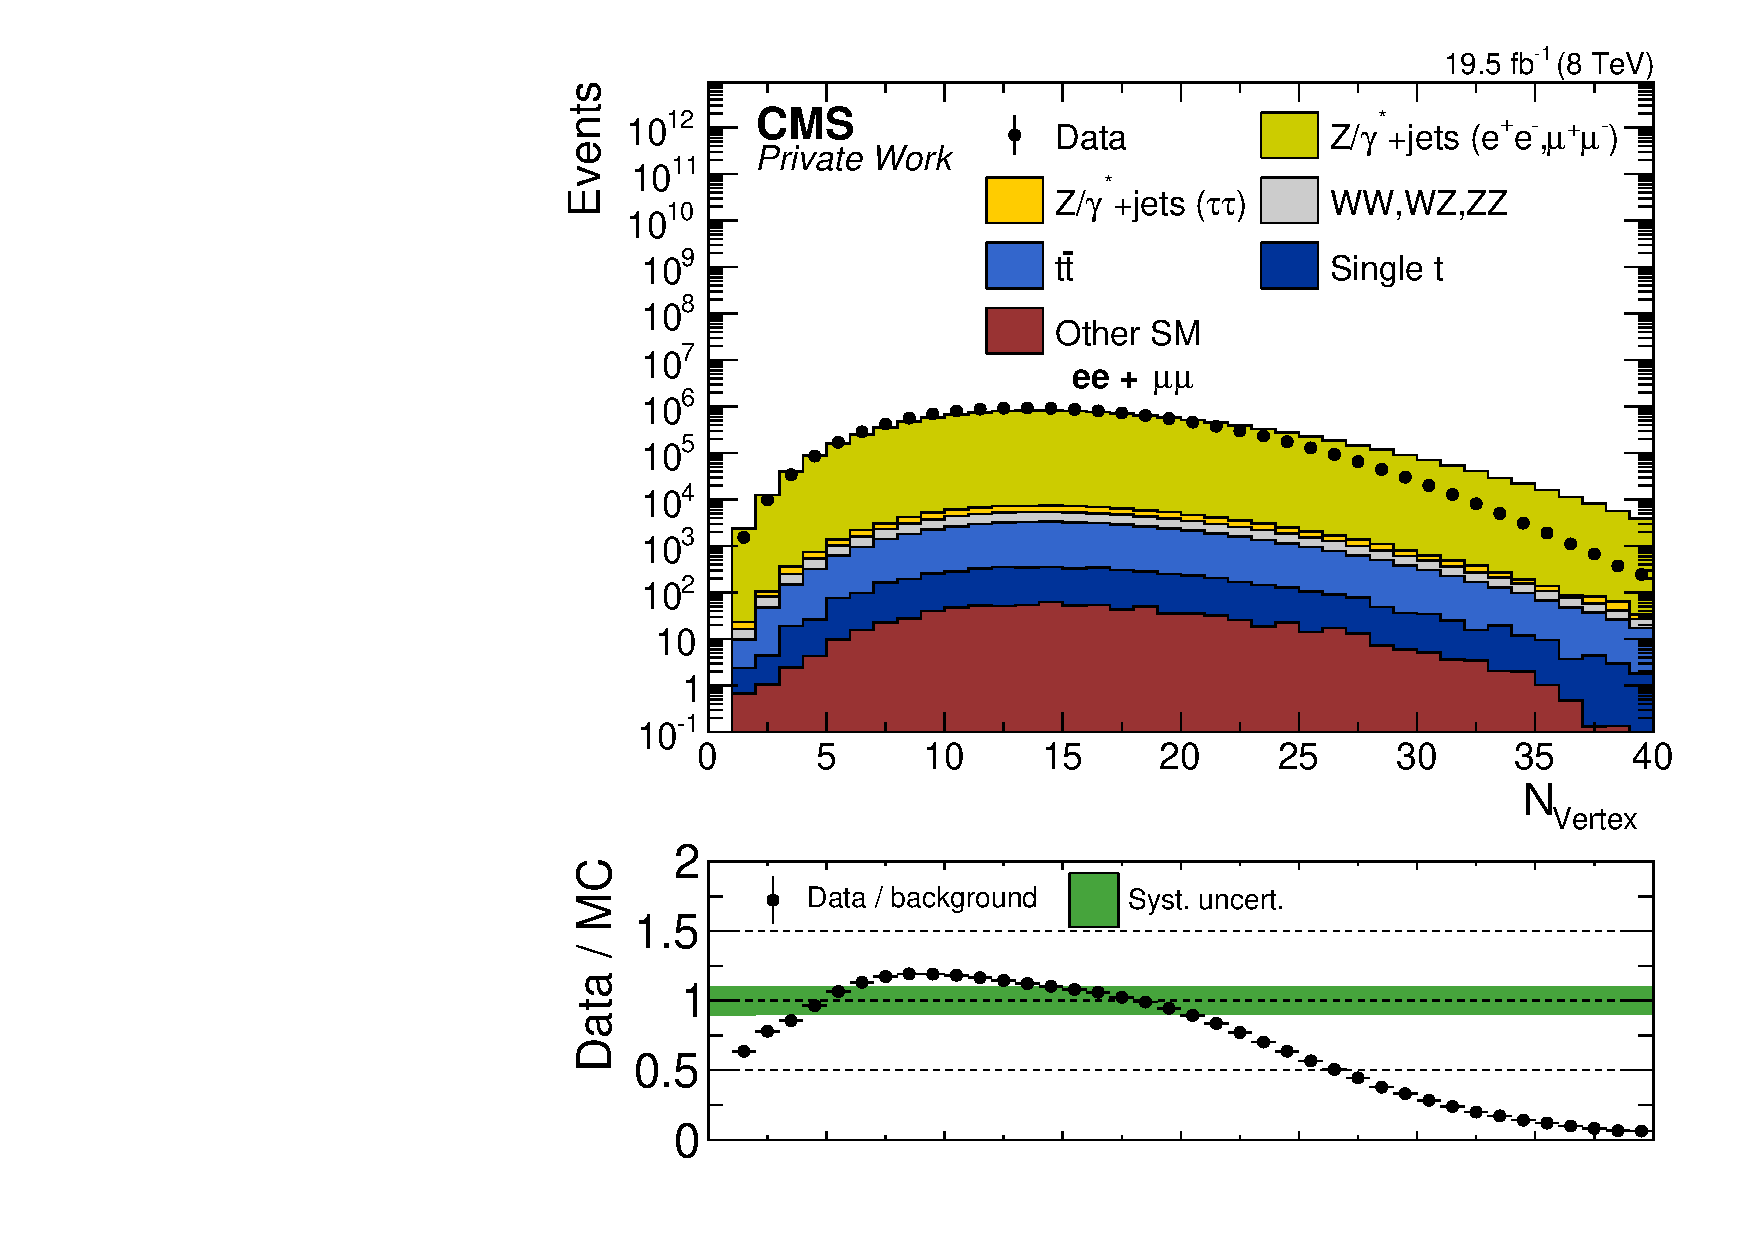
\includegraphics[width=\textwidth]{plots/SELECTION/Inclusive_nVtx_Full2012_SF_TopReweighted_NOPU.pdf}
\end{minipage}
\begin{minipage}[t]{0.49\textwidth}
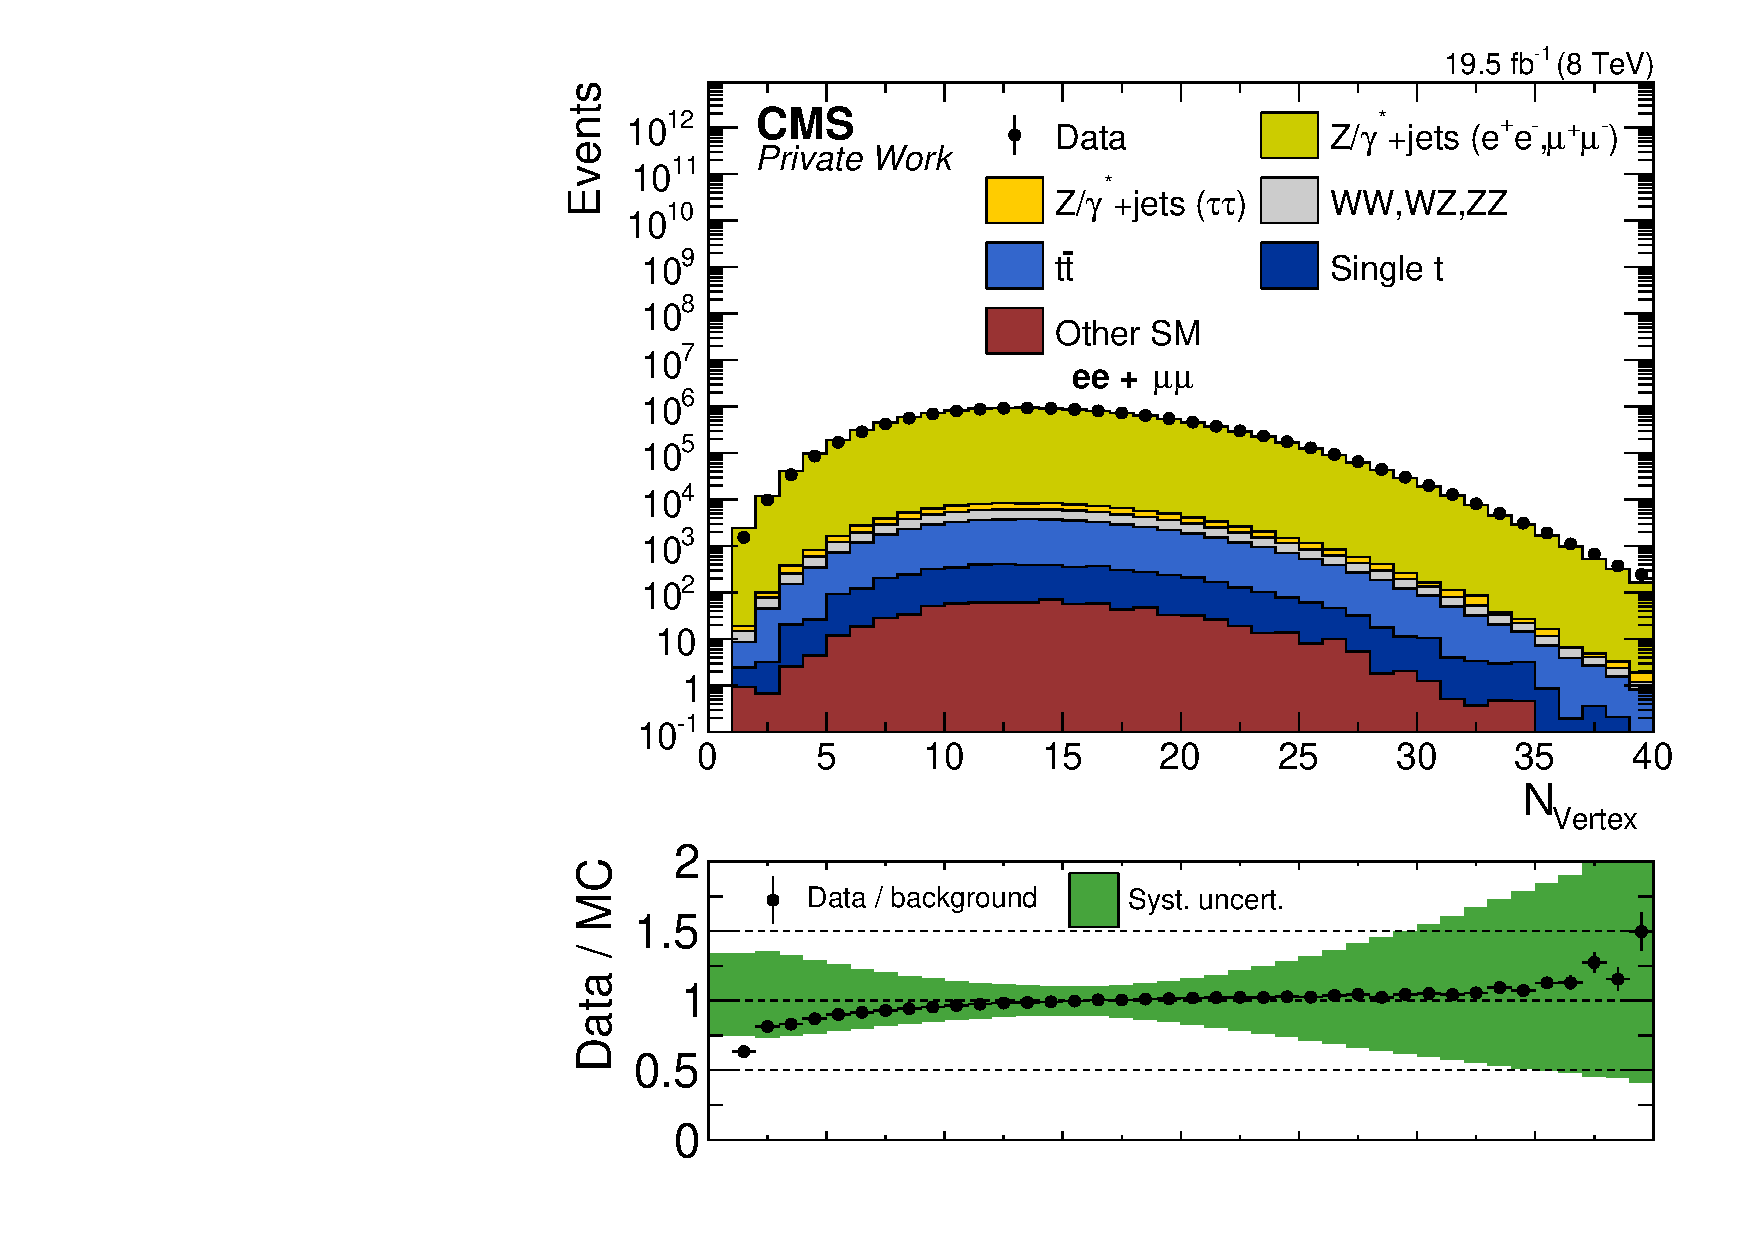
\includegraphics[width=\textwidth]{plots/SELECTION/Inclusive_nVtx_Full2012_SF_TopReweighted.pdf}
\end{minipage}
\caption{Distribution of the number of reconstructed vertices in an inclusive dilepton selection before (left) and after (right) pileup reweighting. The data are shown as black points. The different physical processes contributing to the sample are shown as stacked coloured histograms. Below the plots the ratio of data to simulation is shown. The error bars on the black points include the statistical uncertainties of both data and simulation, while the green band shows the systematic uncertainty on the simulation. }
\label{fig:PU}
\end{figure}   

\subsubsection{Signal datasets}
For simulated signals used in the analysis, initial squark pair production is simulated with Madgraph, including the emission of up to two additional partons at matrix element level. Sparticle decays and parton showers are generated with Pythia. The fast simulation of the CMS detector is used to model the detector response. Details of the physical models have been discussed in Section~\ref{sec:models}.
\section{Event selection}
A series of selection criteria are applied to the events to select signal-like topologies and reduce the contributions from SM backgrounds to the final sample. Also, requirements are defined to select control regions enriched in certain SM processes for the purpose of background prediction and the validation of methods. Additionally, events are rejected that exhibit signs of detector noise or are otherwise not suited for analysis. 

\subsection{Event cleaning}
As a first step in the selection of reconstructed events, a series of quality requirements is applied. 
The quality of the data recorded by the CMS detector is assessed in several automated or manual steps, summarised as $\textit{data quality monitoring (DQM)}$~\cite{DQM}. For each lumi section this results in a binary decision, flagging it as either $\textit{good}$ or $\textit{bad}$, accepting only those lumi sections for which all subdetectors were fully operational during data taking and no problems occurred in the reconstruction of the events.

To reject non-collision events, vertex information is used. The presence of at least one primary vertex is required whose distance to the interaction point is less than $\unit{24}{\centi\meter}$ in $z$ direction and $\unit{2}{\centi\meter}$ in the $x$-$y$ plane. Also, the number of degrees of freedom, defined~\cite{Chatrchyan:2014fea} as:
\begin{equation}
n_{dof} = -3 + 2 \sum\limits_{i=1}^{N_{\text{associated tracks}}} w_i,
\end{equation}
where the $w_i$ are weights assigned to each track based on the likelihood that it is correctly associated with the vertex, is required to be greater than four  

As it relies on the balance of all reconstructed objects, \MET is especially sensitive to detector noise or particles not originating from the proton-proton collisions, which affect the event reconstruction. Several sources of these effects have been identified during the data taking and filters have been developed in CMS to reject events matching their signatures~\cite{CMS-PAS-JME-12-002}. This includes filters for signal produced by interactions of the beam with gas molecules in the beam pipe or of protons in the beam halo with the LHC infrastructure, anomalous noise in the HCAL or ECAL, dead ECAL cells, calibration lasers mistakenly firing during collision events, or failures of the tracking algorithms. The effect of these filters on the tails of the \MET distribution in dijet events is shown in Figure~\ref{fig:METFilters}. Events with \MET larger than $\unit{300}{\giga\electronvolt}$ are dominantly rejected by the filters, greatly improving the agreement between the data and simulation.
\begin{figure}
\begin{center}
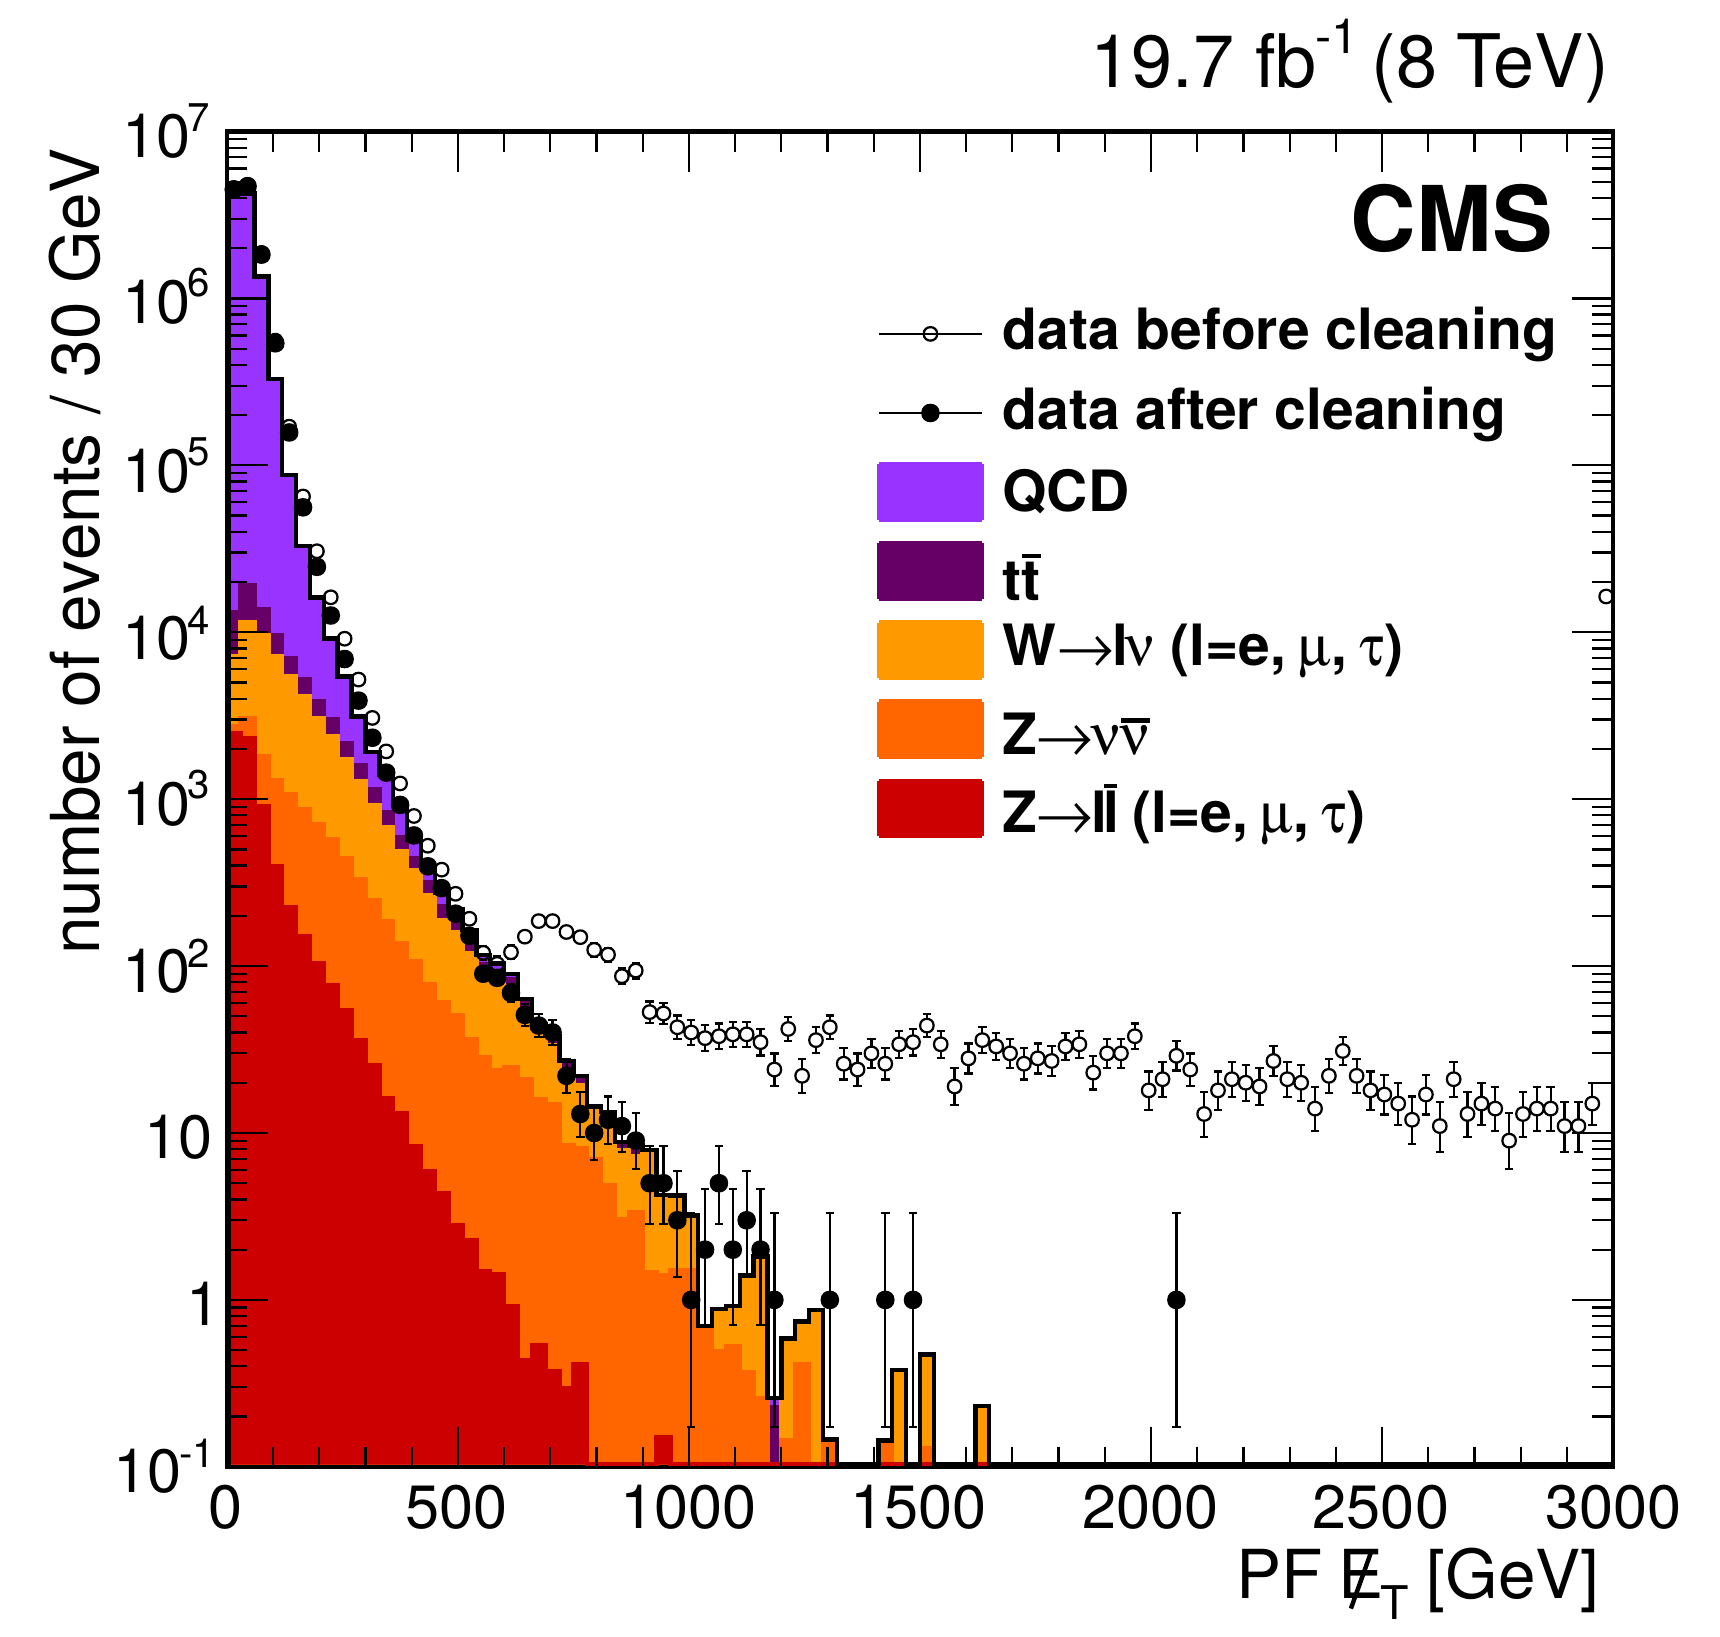
\includegraphics[scale=0.15]{plots/SELECTION/METFilter2.png}
\caption{Distribution of \MET in dijet events in 2012 data. The open data points show all events, while the black points show the data after application of \MET filters. Simulated SM processes are shown as filled histograms~\cite{1748-0221-10-02-P02006}.}
\label{fig:METFilters}
\end{center}
\end{figure}


\subsection{Inclusive dilepton selection}
\label{sec:inclusiveSelection}
In the inclusive dilepton selection, events are selected containing two isolated electrons or muons with opposite electric charge, \pt larger than $\unit{20}{\giga\electronvolt}$, and $|\eta|$ smaller than 2.4. Leptons with $1.4 < \abs{\eta} < 1.6$ are rejected and the event sample is divided into events where both leptons have $\abs{\eta} < 1.4$ (central) and events where at least one lepton has $\abs{\eta} > 1.6$ (forward). The dilepton invariant mass is required to be larger than $\unit{20}{\giga\electronvolt}$ and the two leptons are required to be separated by more than $\Delta R (\ell\ell) = 0.3$. In the signal selection, only events with two same flavour (SF) leptons are considered. Events with opposite flavour (OF) leptons are used to estimate SM backgrounds. These selection requirements are motivated in the following. A summary of this selection and other selection requirements defined in this section is given in Table~\ref{tab:selections}.

The choice of the isolation requirement of $\frac{\text{Iso}}{\pt}< 0.15$ is illustrated in Figure~\ref{fig:isolation} (left), where the distribution of the relative isolation is shown for the trailing lepton in \ttbar simulation in the inclusive dilepton selection. Using the truth information of the simulation the sample is split into prompt leptons originating from \W boson decays, leptons originating from heavy flavour hadron decays inside b-quark jets, and jets misreconstructed as leptons. The prompt leptons are concentrated at very low values, but a long tail extends to much higher values. The leptons from heavy flavour decays are less well isolated, with a broad maximum of the distribution between 0.5 and 1. Misreconstructed leptons are spread more evenly between high and low values of isolation. The cut value of 0.15 allows for a strong suppression of non-prompt leptons while a high efficiency is retained for prompt leptons. The isolation efficiency as a function of the number of reconstructed vertices is shown on the right side of Figure~\ref{fig:isolation} separately for prompt electrons and muons in \ttbar and \zjets events. The efficiency in \zjets evens is about 5 percentage points higher compared to the more hadronic environment of \ttbar events. While the efficiency for electrons shows only a slight dependency on the number of vertices and therefore on the amount of pileup, for muons a more strong decrease of efficiency is observed for high numbers of vertices. However, for \ttbar events this is much less pronounced, as the efficiency is already diminished by the higher number of jets in this environment. The good separation of prompt and non-prompt leptons and the high efficiency for prompt leptons are therefore  retained even in the challenging conditions of high pileup. 

\begin{figure}[htbp]
\centering
\begin{minipage}[t]{0.49\textwidth}
  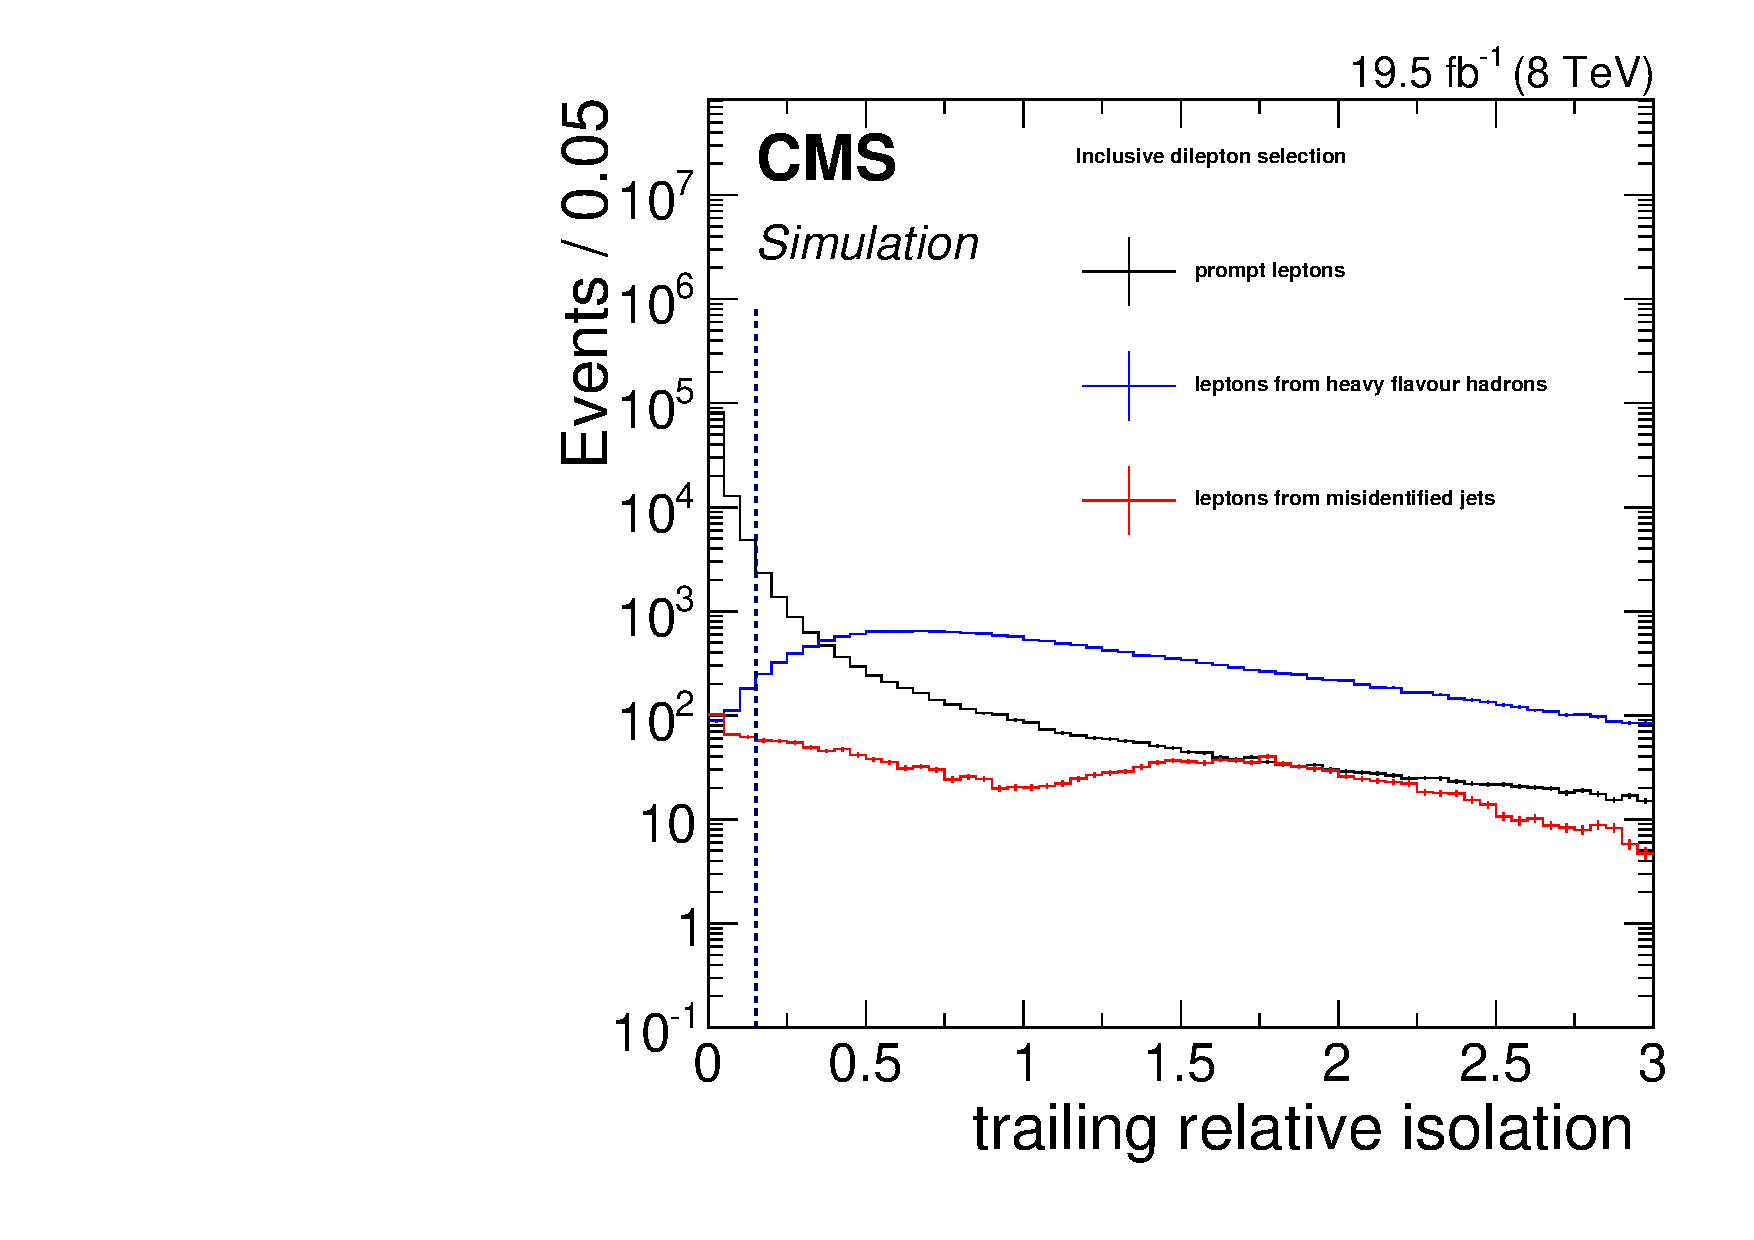
\includegraphics[width=\textwidth]{plots/SELECTION/iso_Inclusive_Full2012_TrailingIso_None_MC.pdf}
\end{minipage}
\begin{minipage}[t]{0.49\textwidth}
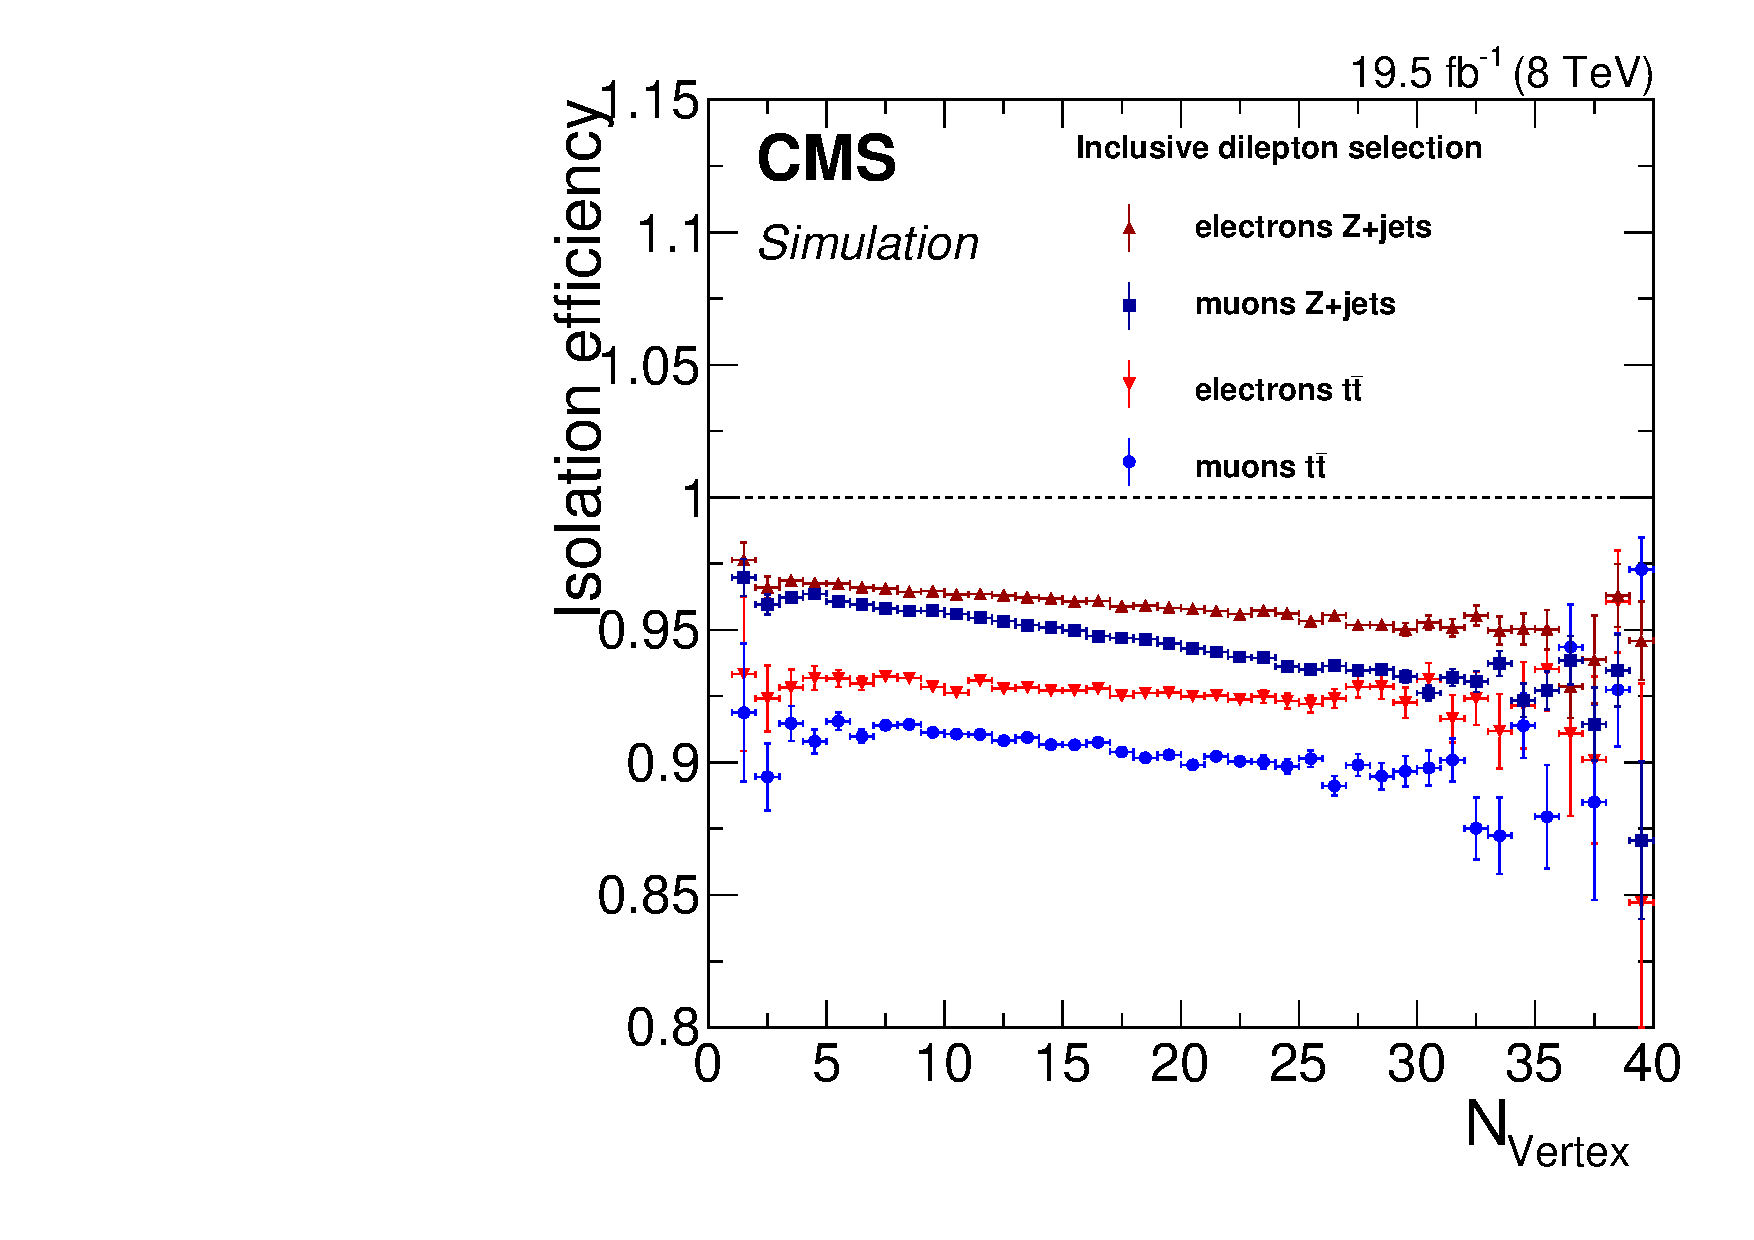
\includegraphics[width=\textwidth]{plots/SELECTION/isoEff_Inclusive_Full2012_nVtx_None_MC.pdf}
\end{minipage}
\caption{On the left, the distribution of the pileup corrected relative isolation of the trailing lepton for prompt leptons, leptons from heavy flavour decays, and misidentified jets in \ttbar simulation is shown. On the right side, the efficiency for a prompt lepton to pass the isolation requirement is shown as a function of the reconstructed number of vertices for both \ttbar and \Zjets simulation. In both cases, the inclusive dilepton selection is applied.}
\label{fig:isolation}
\end{figure}   

The \pt requirement is driven by the thresholds of the dilepton triggers, as discussed in Section~\ref{sec:triggerEffs}, while the $|\eta|$ restriction is imposed  by the coverage of the muon system. The acceptance for electrons could in principle be extended to $|\eta| =$ 2.5, but is chosen to be the same for both lepton flavours. Lepton pairs are required to be selected by the corresponding trigger, e.g. an event containing a pair of electrons has to have fired the dielectron trigger. If there is more than one pair of leptons fulfilling this basic requirements in one event, the pair with the largest scalar sum of lepton \pt is chosen. There is no explicit requirement of the two selected leptons to be matched to the objects that fired the trigger.

As the symmetry between lepton flavours is a key ingredient of the methods to estimate the backgrounds from SM processes, parts of the detector acceptance for which these symmetries are potentially violated are excluded.

As the efficiency to reconstruct electrons is reduced in the overlap region between the barrel and endcap detectors of the ECAL, the relative event yield for events with electrons with $|\eta|$ between 1.4 and 1.6 is reduced compared to those with muons in this range. This distribution of the $|\eta|$ of the leading lepton in \EE and  \MM events is shown in Figure~\ref{fig:cutJustification} (left), illustrating the greatly increased difference between the event yields for electrons and muons in the overlap region. Events containing a lepton with a pseudorapidity of $1.4<|\eta|<1.6$ are therefore rejected. Also, an increasing difference between electrons and muons can be seen for events were the leading leptons is in the endcap region of the detector. This motivates the split of the event samples into the two categories central, where both leptons are reconstructed with $|\eta| < 1.4$ and forward, where at least one leptons has to be reconstructed with $|\eta| > 1.6$. Also, the decay products of heavy SUSY particles are expected to be located dominantly in the central detector region, as the initially produced sparticles are not significantly boosted into the forward direction. The efficiency drop for muons around $|\eta| = 0.25$ is caused by the transition between different DT chambers in the muon system~\cite{CMS}. While there are several of these transitions, the effect is most pronounced at low $\abs{\eta}$ because the angle between the trajectory of the muon and the gap between the chambers is smaller.

Leptons with small spatial separation can interfere with each other's reconstruction and isolation. These effects are different for electrons and muons, which can be seen in Figure~\ref{fig:cutJustification} (right). The ratio of electrons to muons first rises for lower values of $\Delta R(\ell\ell)$ before dropping for values below $0.1$. The leptons are therefore required to be separated in $\Delta R(\ell\ell)$ by more than 0.3. Some differences between electrons and muons can also be observed for very high values of $\Delta R(\ell\ell)$, but they are less pronounced and this region is less populated.  

\begin{figure}[htbp]
\centering
\begin{minipage}[t]{0.49\textwidth}
  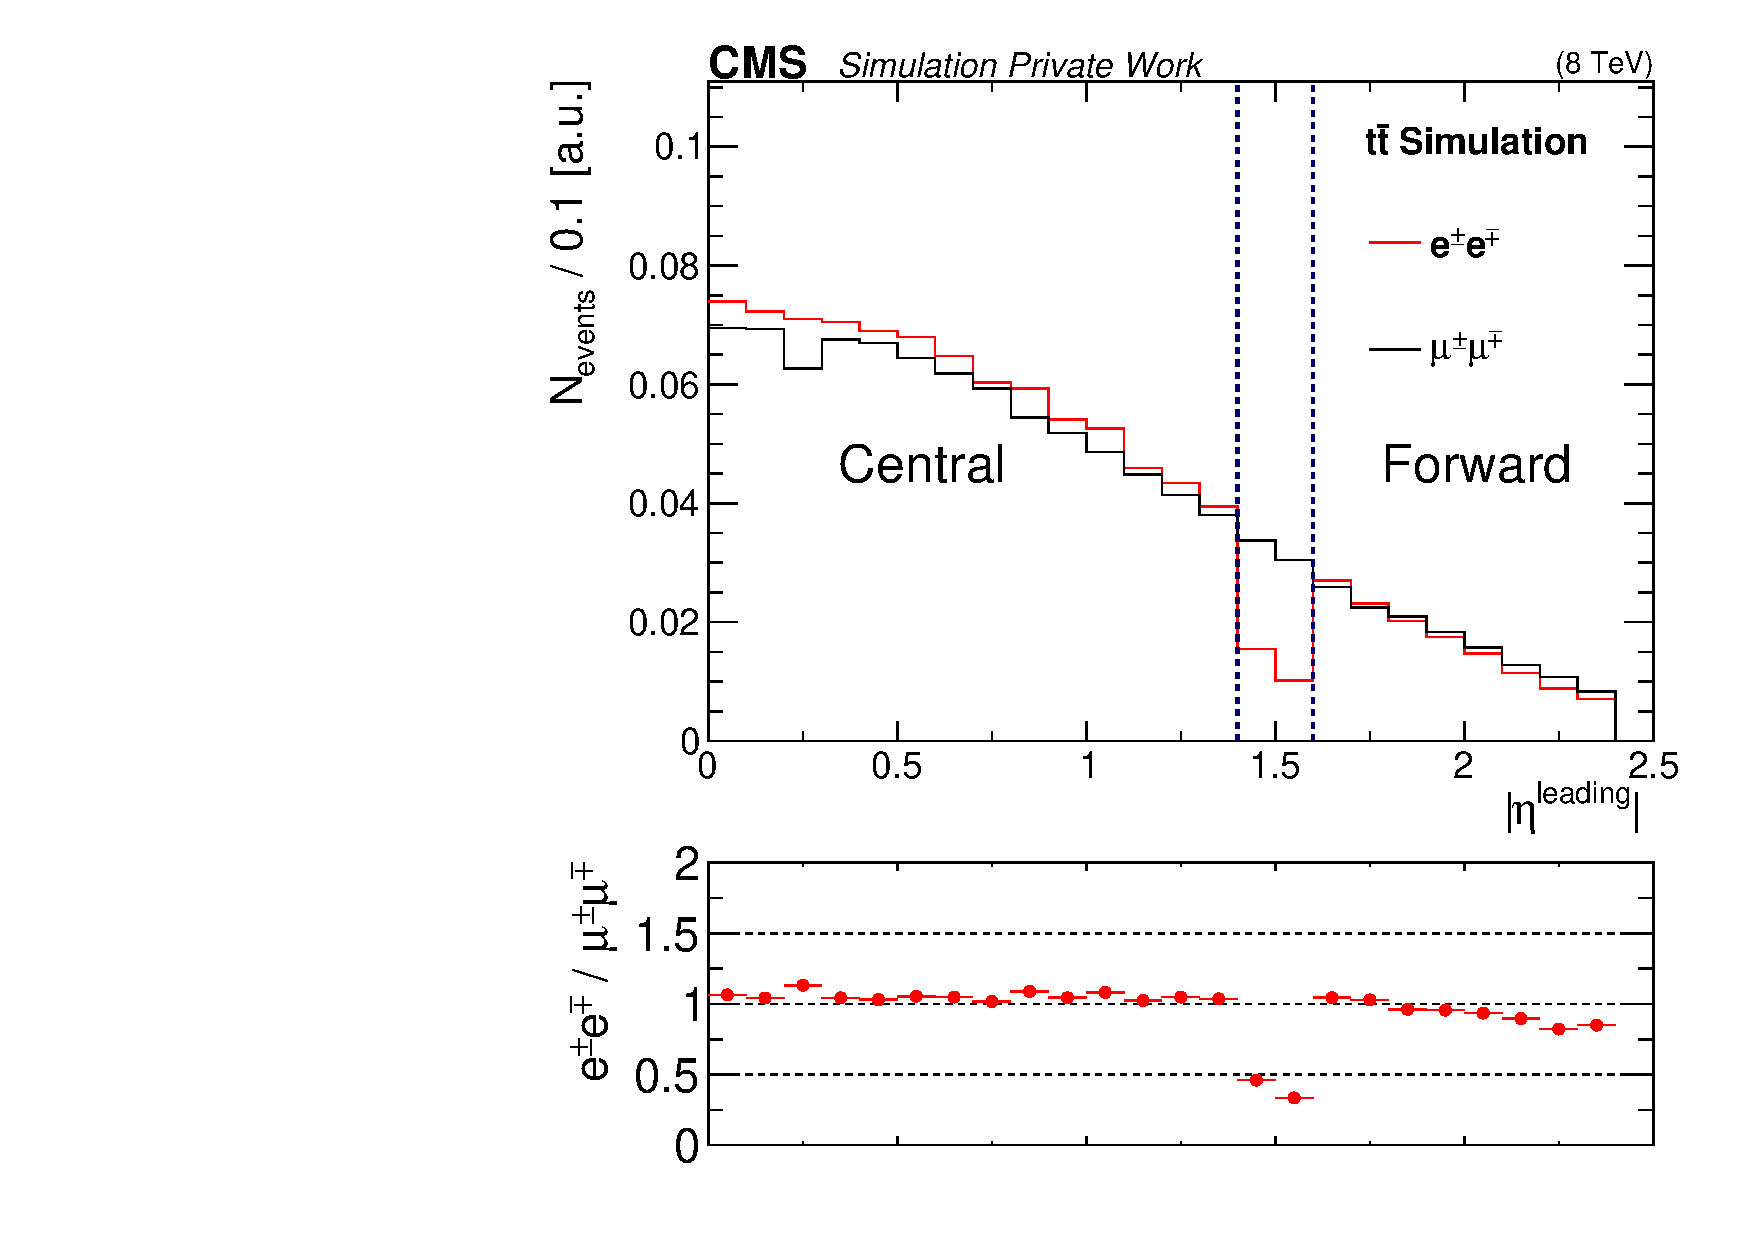
\includegraphics[width=\textwidth]{plots/SELECTION/gapJustification.pdf}
\end{minipage}
\begin{minipage}[t]{0.49\textwidth}
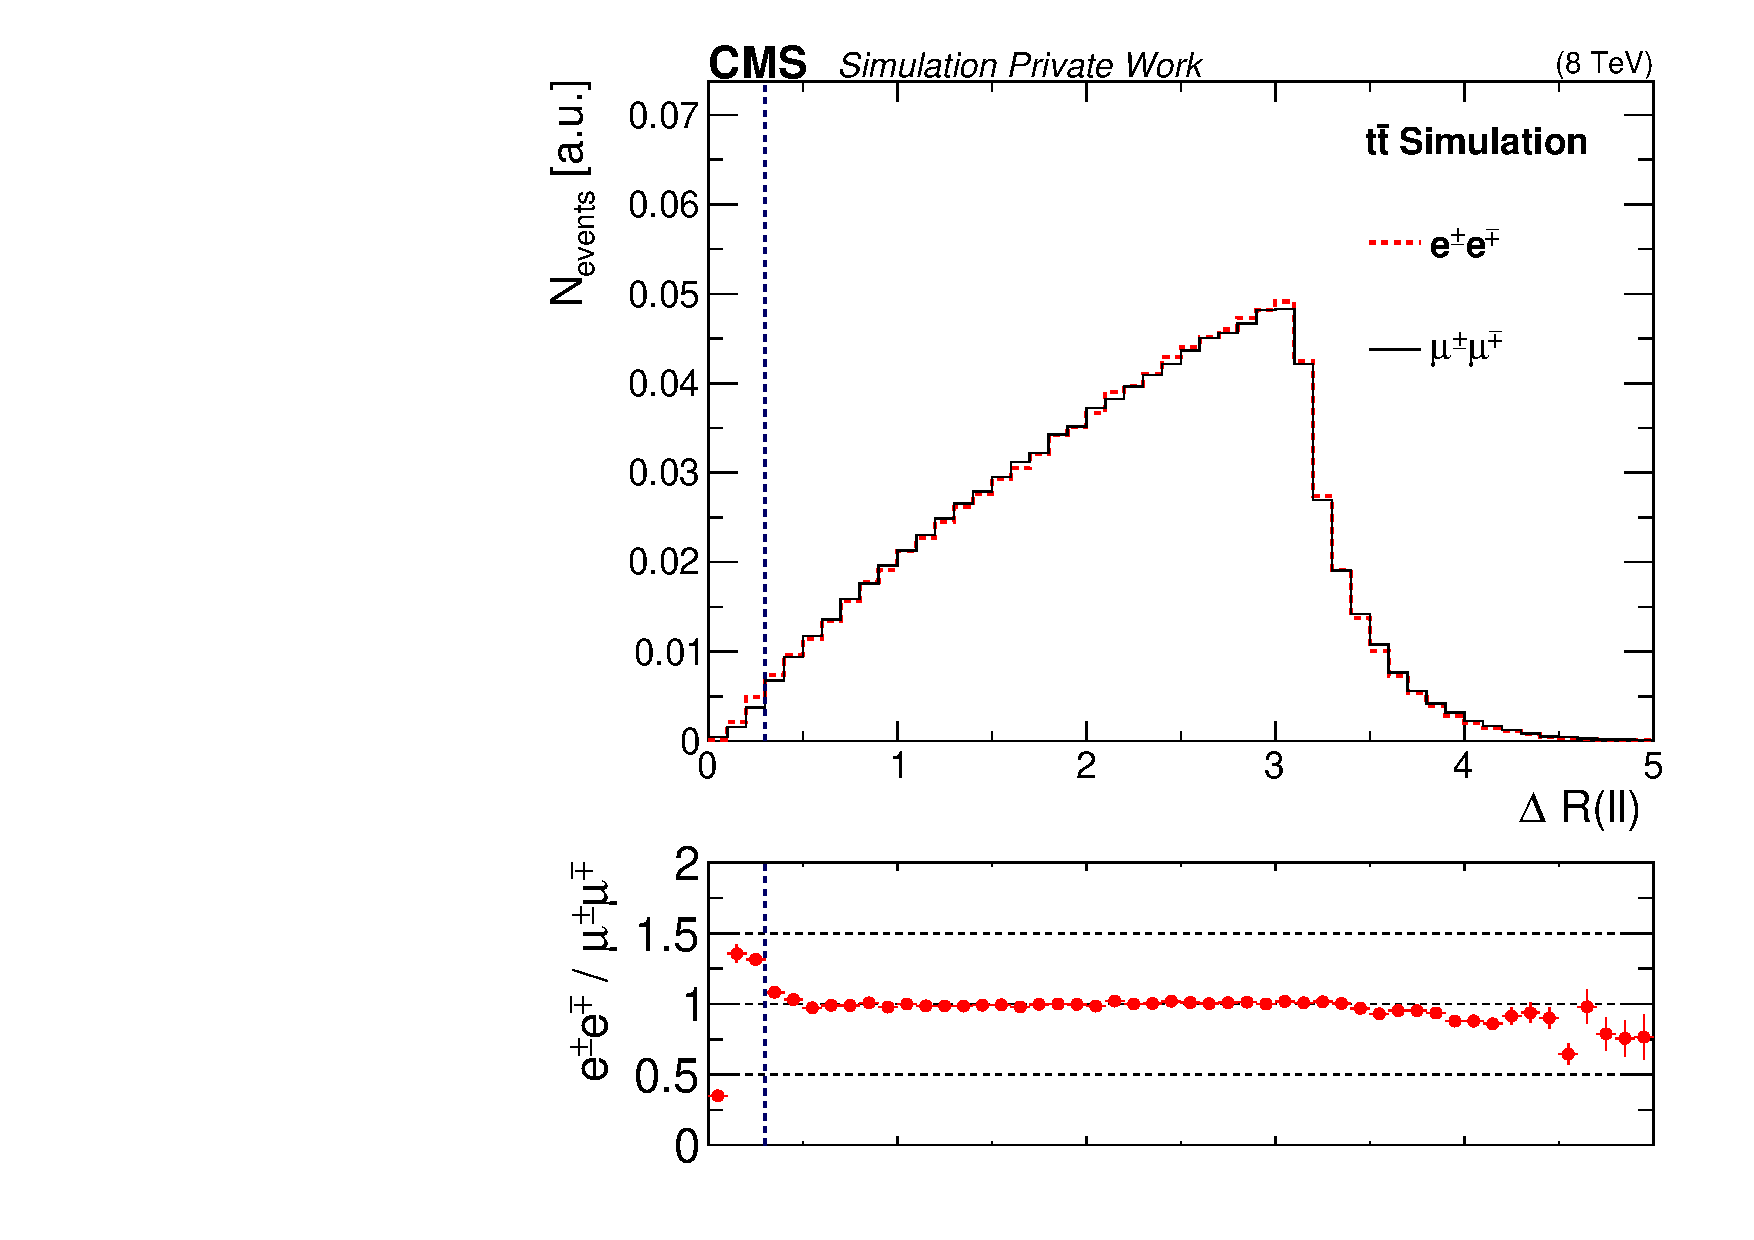
\includegraphics[width=\textwidth]{plots/SELECTION/dRJustification_eeVSmm.pdf}
\end{minipage}
\caption{Distributions of $|\eta|$ (left) and $\Delta R(\ell\ell)$ (right) for the leading lepton for \MM (black line) and \EE (red dashed line) events in a simulation of $t\bar{t}$ events. Both histograms have been normalised to an area of 1.}
\label{fig:cutJustification}
\end{figure}    

To avoid possible reconstruction problems and contamination from dilepton production in the decay of bottonium resonances, the dilepton invariant mass \mll is required to be greater than $\unit{20}{\giga\electronvolt}$. 


\subsection{Selections in \MET and jet multiplicity}
\label{sec:regions}
Three subsets of the event sample obtained with the inclusive dilepton selection are defined, resulting in samples enriched by different processes. The variables used in the definitions of these regions are \MET and the number of selected jets \njets. The selections are illustrated in the plots of Figure~\ref{fig:sigRegionBG}, which also show the distribution of $t\bar{t}$ (left) and \Zjets (right) events in the \MET-\njets plane for SF leptons. 
 
The signal region, in which the search is performed, is defined by requiring either $\njets \geq 3$ and $\MET > \unit{100}{\giga\electronvolt}$; or $\njets \geq 2$ and $\MET > \unit{150}{\giga\electronvolt}$. This definition allows to select signal events for points in the parameter space where more energy is distributed to the jets and less to the invisible component of the signature and vice versa. At the same time the rejection of background events with both lower $N_{jets}$ and \MET is maintained. A control region dominated by flavour-symmetric processes is defined by selecting events with $\njets = 2$ and $\unit{100}{\giga\electronvolt} < \MET < \unit{150}{\giga\electronvolt}$. 

To study lepton pairs produced via the Drell-Yan process and to obtain a high statistics sample of leptons for efficiency measurements, events with $\njets \geq 2$ and $\MET < \unit{50}{\giga\electronvolt}$ are selected. This allows to select events with kinematics close to those of the signal selection in terms of jet multiplicity. The $\njets$ requirement greatly reduces the statistics and the purity of this event sample. However, because of the large cross section of the Drell-Yan process, the event yield is still sufficient for the purposes of this analysis and Drell-Yan events dominate over those from $t\bar{t}$ production by two orders of magnitude.
\begin{figure}[htbp]
\centering
\begin{minipage}[t]{0.49\textwidth}
  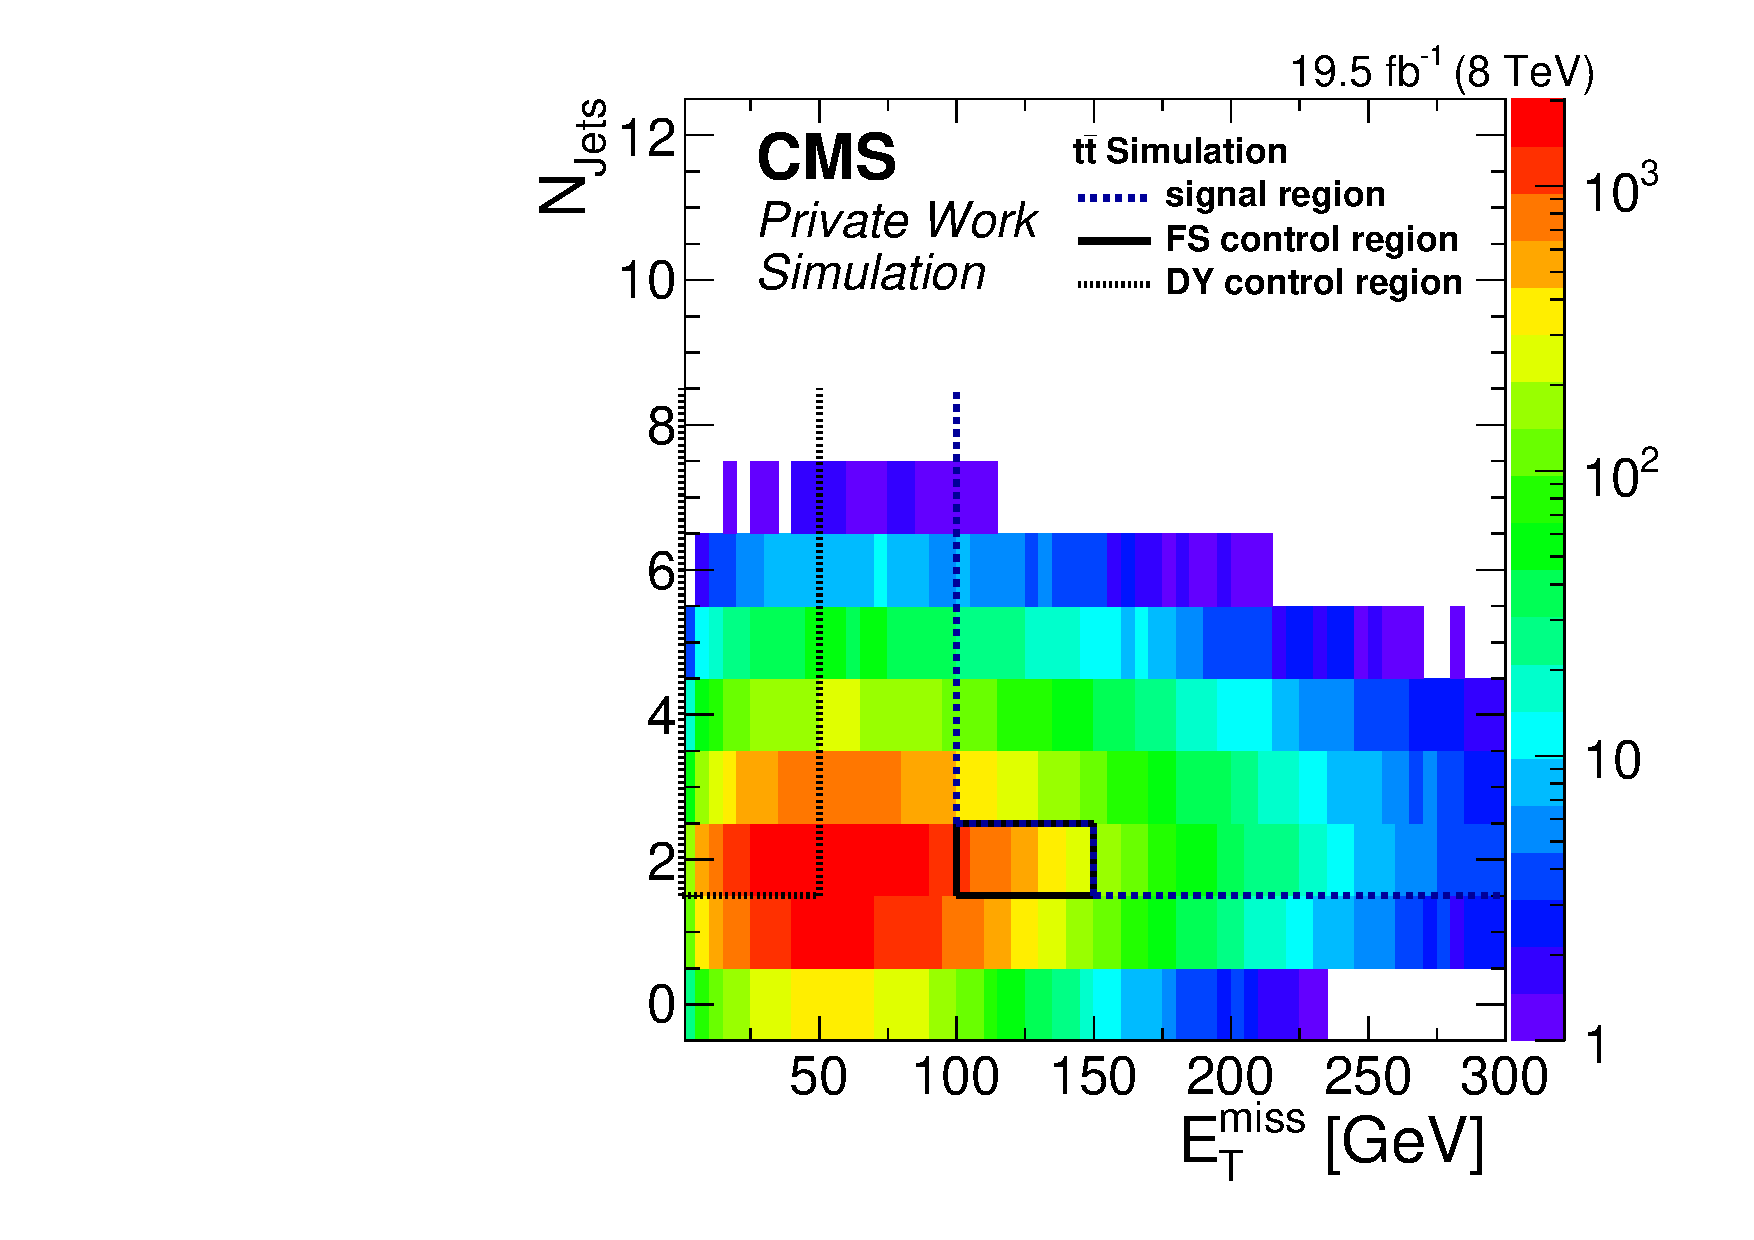
\includegraphics[width=\textwidth]{plots/SELECTION/metJetsScatter_ttbar.pdf}
\end{minipage}
\begin{minipage}[t]{0.49\textwidth}
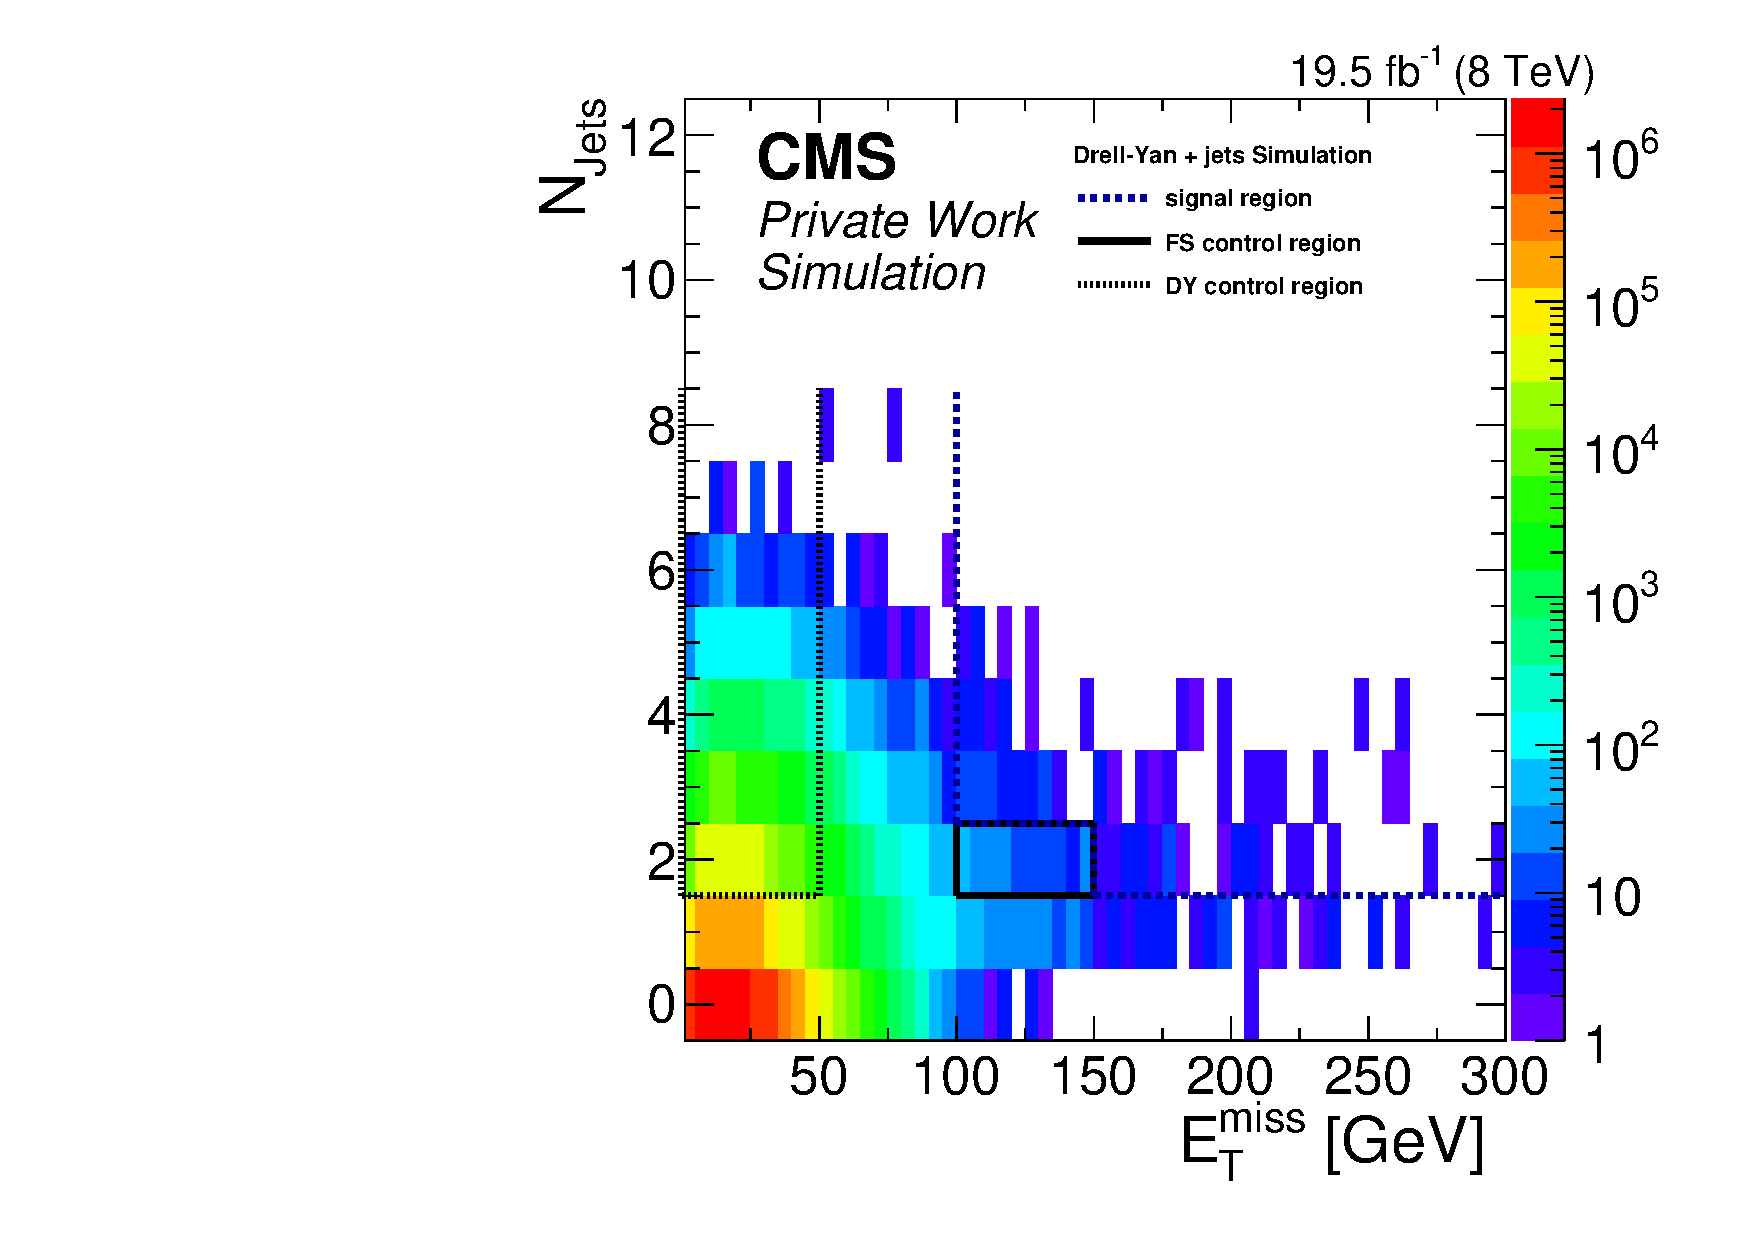
\includegraphics[width=\textwidth]{plots/SELECTION/metJetsScatter_DY.pdf}
\end{minipage}
\caption{Distribution of backgrounds events with SF leptons in the \MET-\njets plane for $t\bar{t}$ (left) and Drell-Yan (right) events from simulation. The events are weighted according to the cross section of the process and the size of the generated event sample, assuming an integrated luminosity of \lumi. The three regions defined in the plane are indicated by lines. The central and forward dilepton selections are combined.}
\label{fig:sigRegionBG}
\end{figure}  
  
For comparison the same distributions are shown for two signal points from the models discussed in Section~\ref{sec:models} in Figure~\ref{fig:sigRegionSignal}. On the left a point from the fixed-edge model with $m_{\sbottom} = \unit{550}{\giga\electronvolt}$ and $m_{\secondchi} = \unit{275}{\giga\electronvolt}$ and on the right a point from the slepton-edge model with $m_{\sbottom} = \unit{500}{\giga\electronvolt}$ and $m_{\secondchi} = \unit{175}{\giga\electronvolt}$ is shown. For both signal points almost no events are observed with $\njets < 2$, which is expected because at least two b-jets are produced in each event. Compared to the backgrounds, a clear tendency towards higher \MET and \njets is observed. However, also contributions to the two control regions are present, but they are small compared to the background contributions. Overall, the chosen selection offers a good separation of signal and backgrounds.
\begin{figure}[htbp]
\centering
\begin{minipage}[t]{0.49\textwidth}
  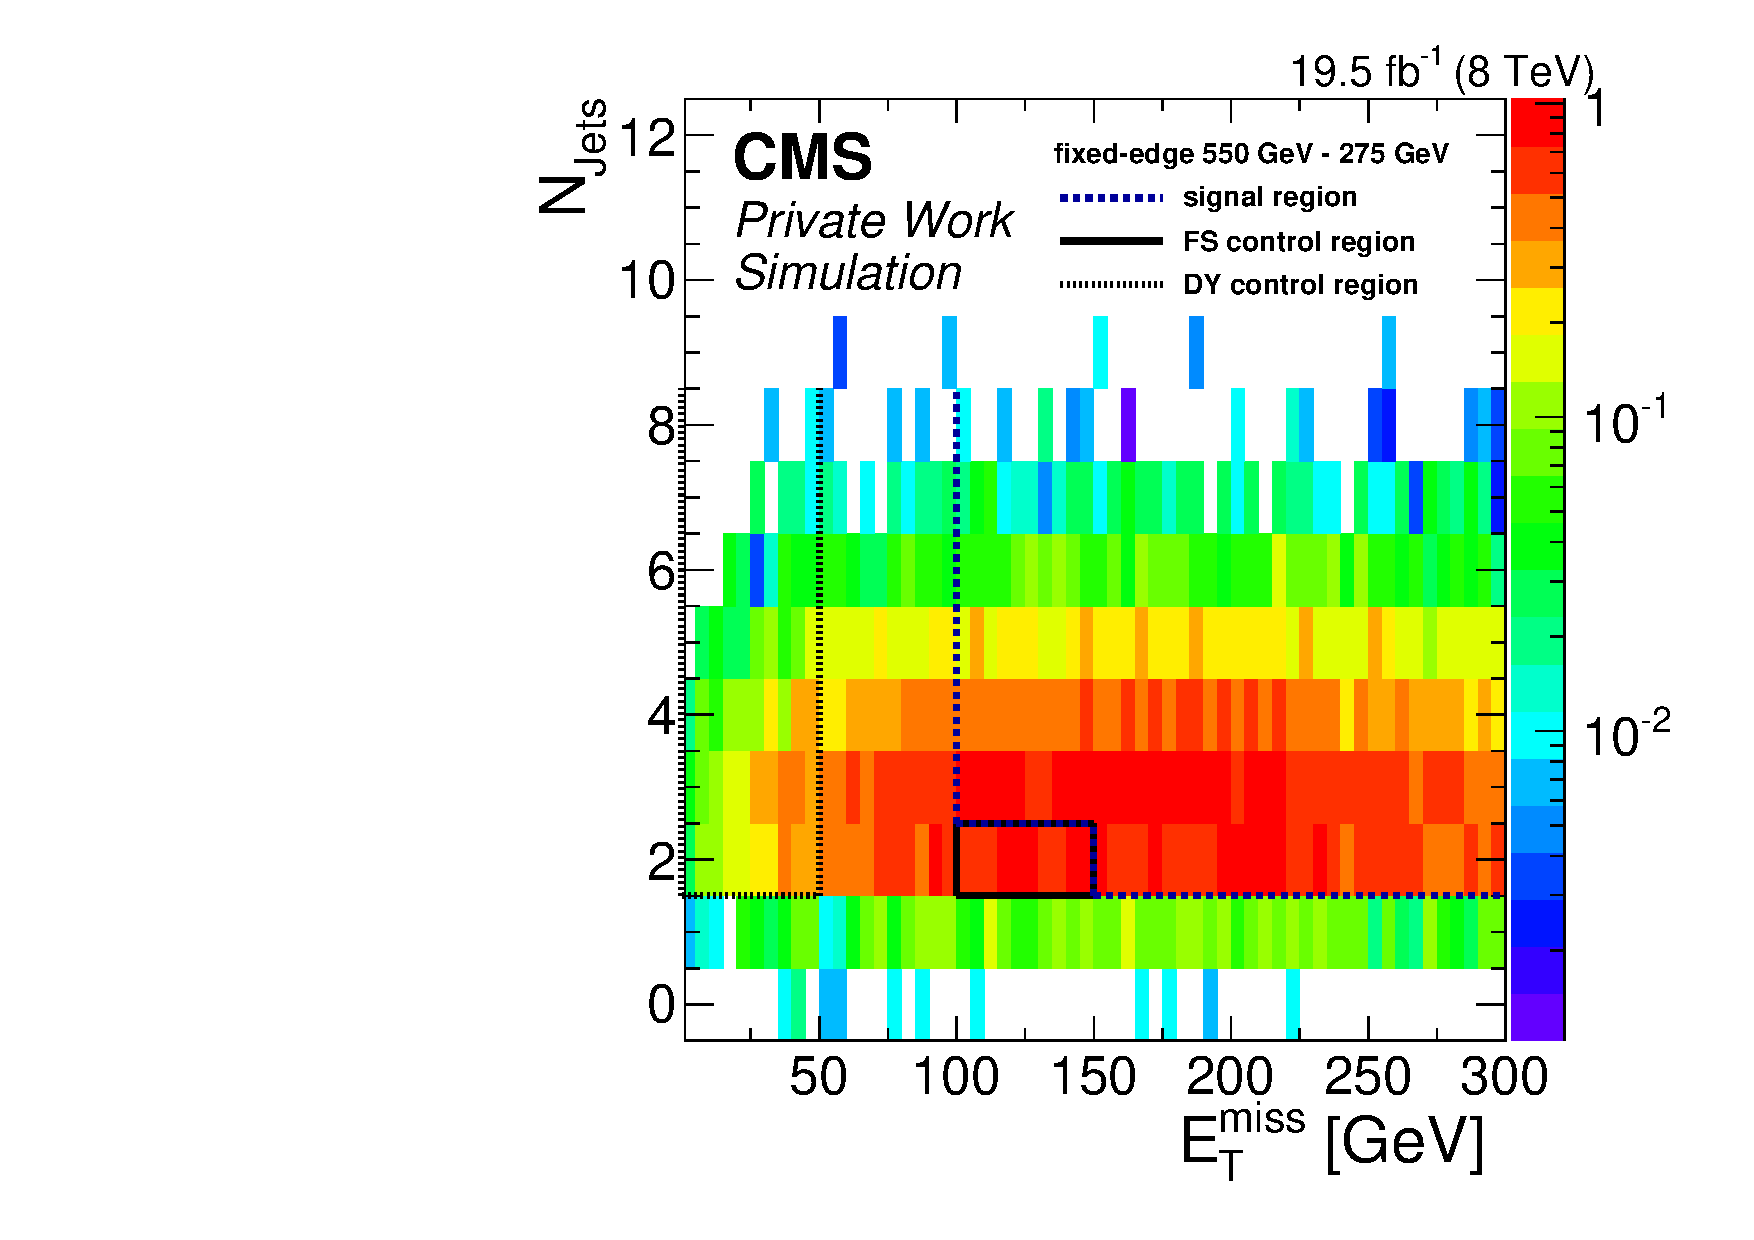
\includegraphics[width=\textwidth]{plots/SELECTION/metJetsScatter_SUSY_edge_550_275.pdf}
\end{minipage}
\begin{minipage}[t]{0.49\textwidth}
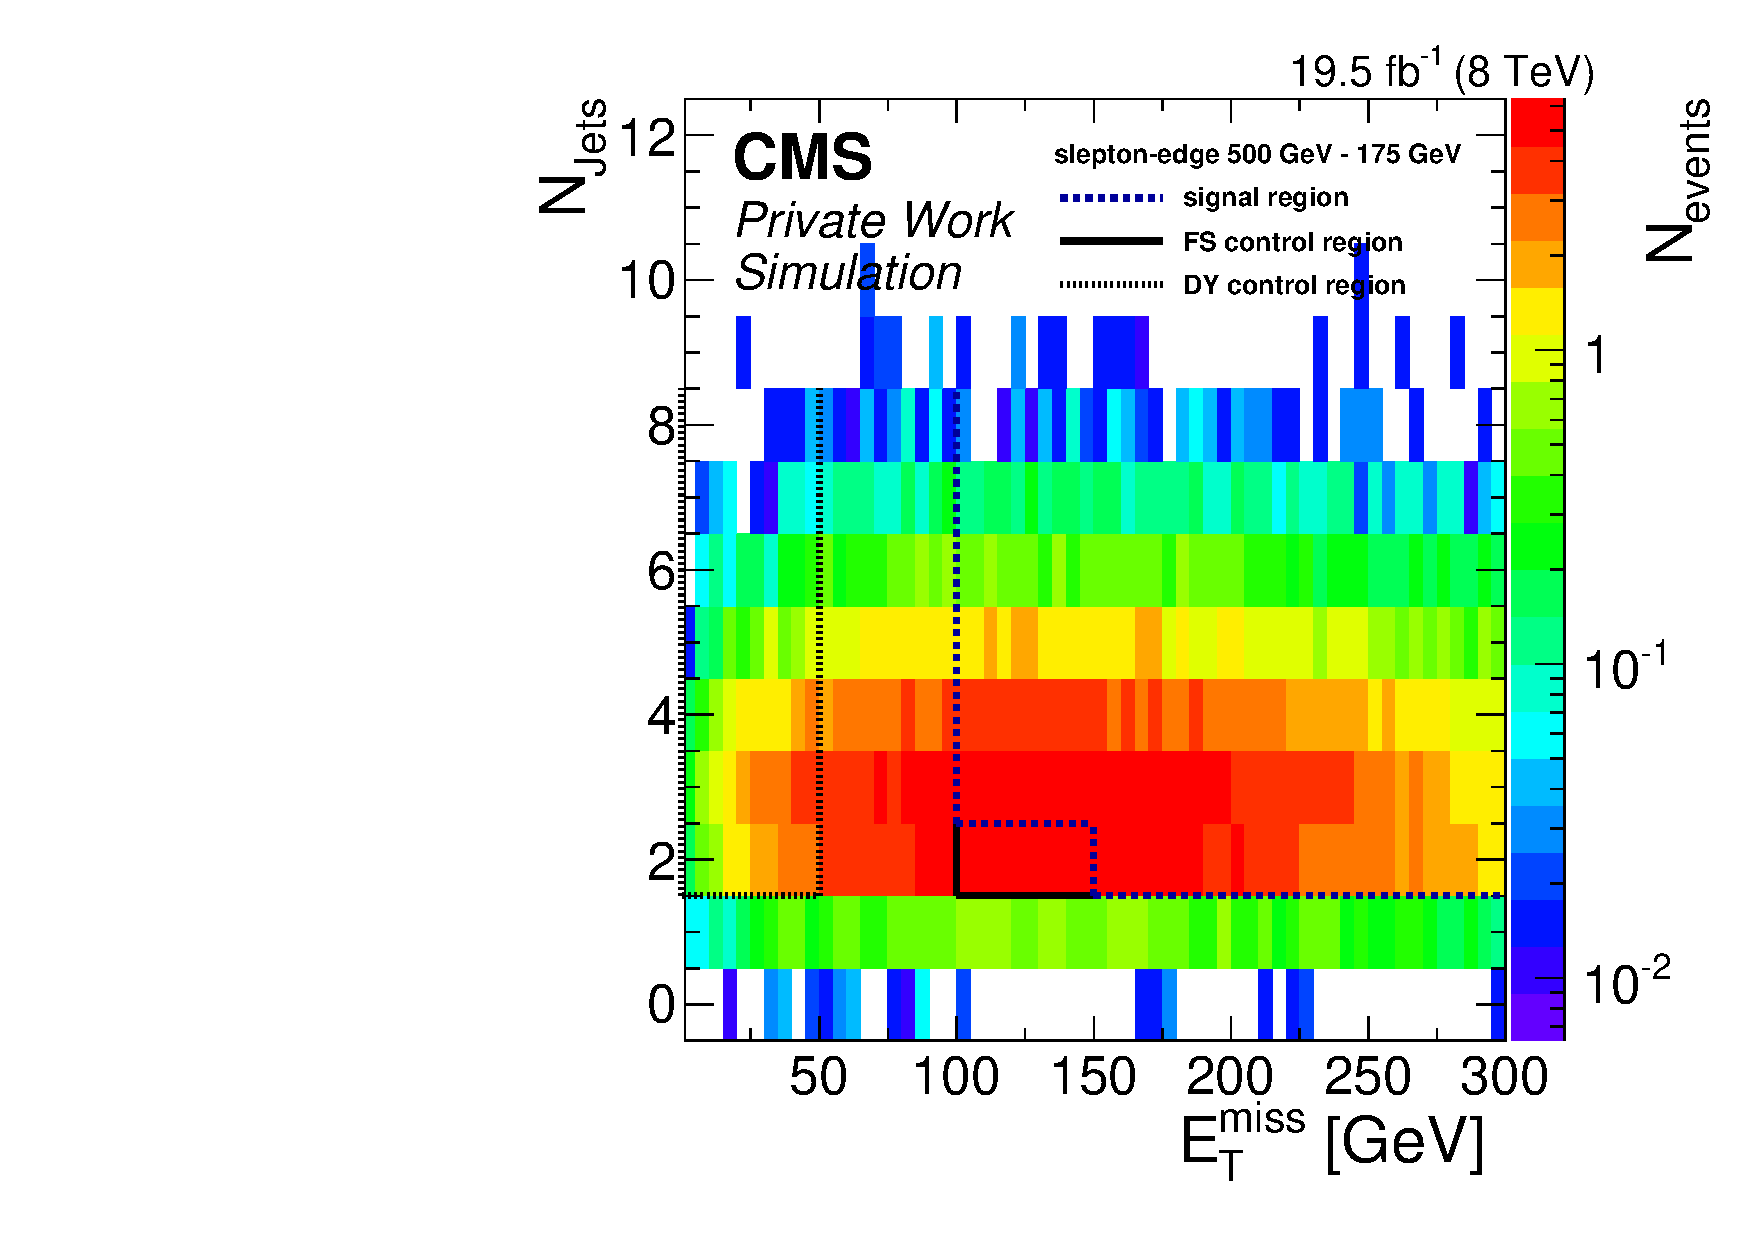
\includegraphics[width=\textwidth]{plots/SELECTION/metJetsScatter_SUSY_slepton_500_175.pdf}
\end{minipage}
\caption{Distribution of signal events with SF leptons in the \MET-\njets plane. Shown is one point from the fixed-edge model with $m_{\sbottom} = \unit{550}{\giga\electronvolt}$ and $m_{\secondchi} = \unit{275}{\giga\electronvolt}$ (left) and one from the slepton-edge model with $m_{\sbottom} = \unit{500}{\giga\electronvolt}$ and $m_{\secondchi} = \unit{175}{\giga\electronvolt}$ (right). The events are weighted according to their cross section and the size of the generated event sample, assuming an integrated luminosity of \lumi. The three regions defined in the plane are indicated by lines. The central and forward dilepton selections are combined.}
\label{fig:sigRegionSignal}
\end{figure}    

\subsection{Selections in \mll}
Since the analysis is performed using two different approaches, a ``counting experiment'' and a shape analysis, several regions are defined in \mll. In the counting experiment, an excess in the number of observed events over the background expectation is sought in three regions of dilepton invariant mass \mll: low-mass ($\mathrm{20}< \mll < \unit{70}{\giga\electronvolt}$), on-\Z ($\mathrm{80}< \mll < \unit{101}{\giga\electronvolt}$) and high-mass ($\unit{120}{\giga\electronvolt} < \mll$). The scope of the counting experiment evolved from a focus on the low mass region to also consider the on-Z and high-mass region, which had been used in the background prediction and as a cross-check before. To keep the event selection stable after starting to analyse the observed data, the gaps between the regions have been retained. Figure~\ref{fig:sigMC} shows the \mll distribution in the central (forward) region on the left (right) for simulated SM backgrounds, which are shown separately for different physics processes. It can be seen that \ttbar is the dominant background in all three mass bins. For the on-\Z region also Drell--Yan backgrounds contribute significantly. The precise determination of these backgrounds from data are described in Section~\ref{sec:backgrounds} and the results of the counting experiment are discussed in Section~\ref{sec:counting}.

\begin{figure}[htbp]
\centering
\begin{minipage}[t]{0.49\textwidth}
  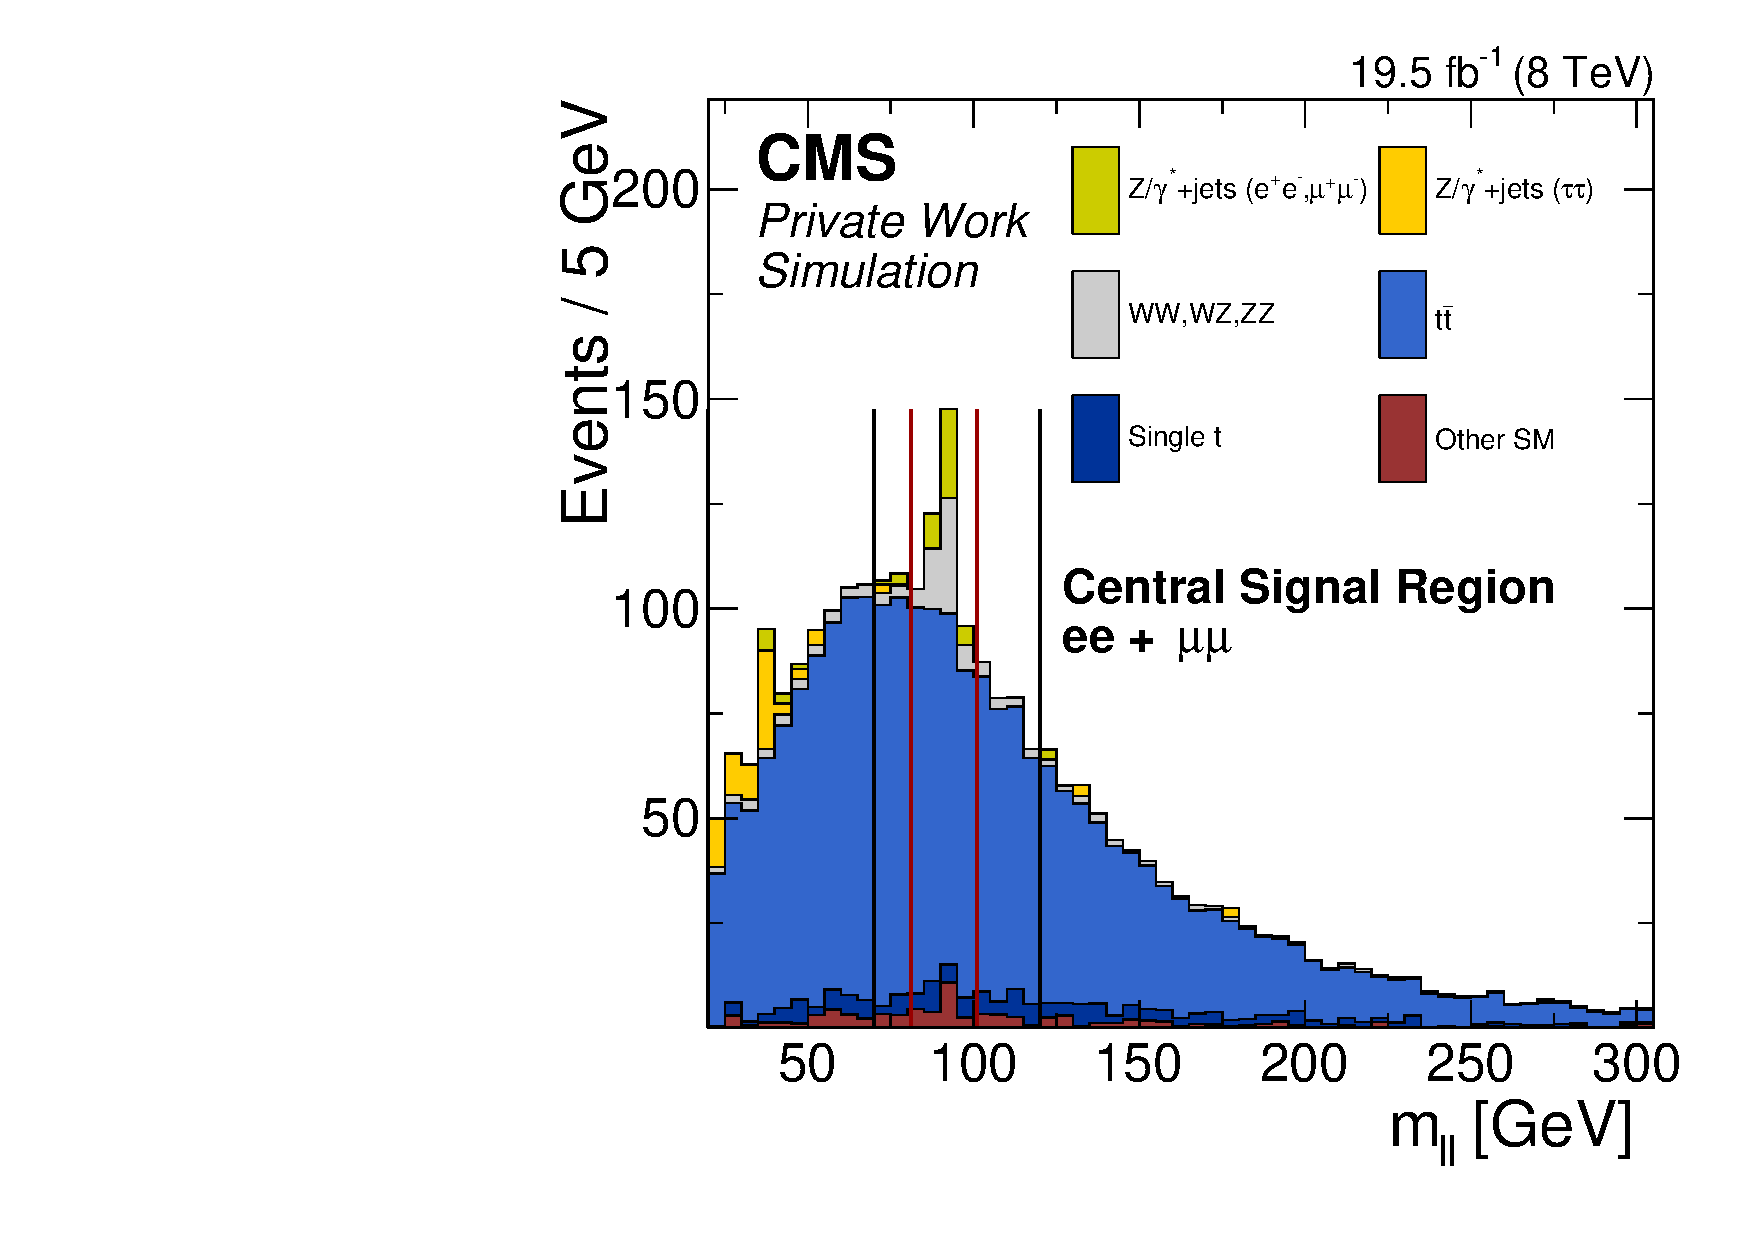
\includegraphics[width=\textwidth]{plots/SELECTION/SignalCentral_Mll_Full2012_SF_TopReweighted_MCOnly.pdf}
\end{minipage}
\begin{minipage}[t]{0.49\textwidth}
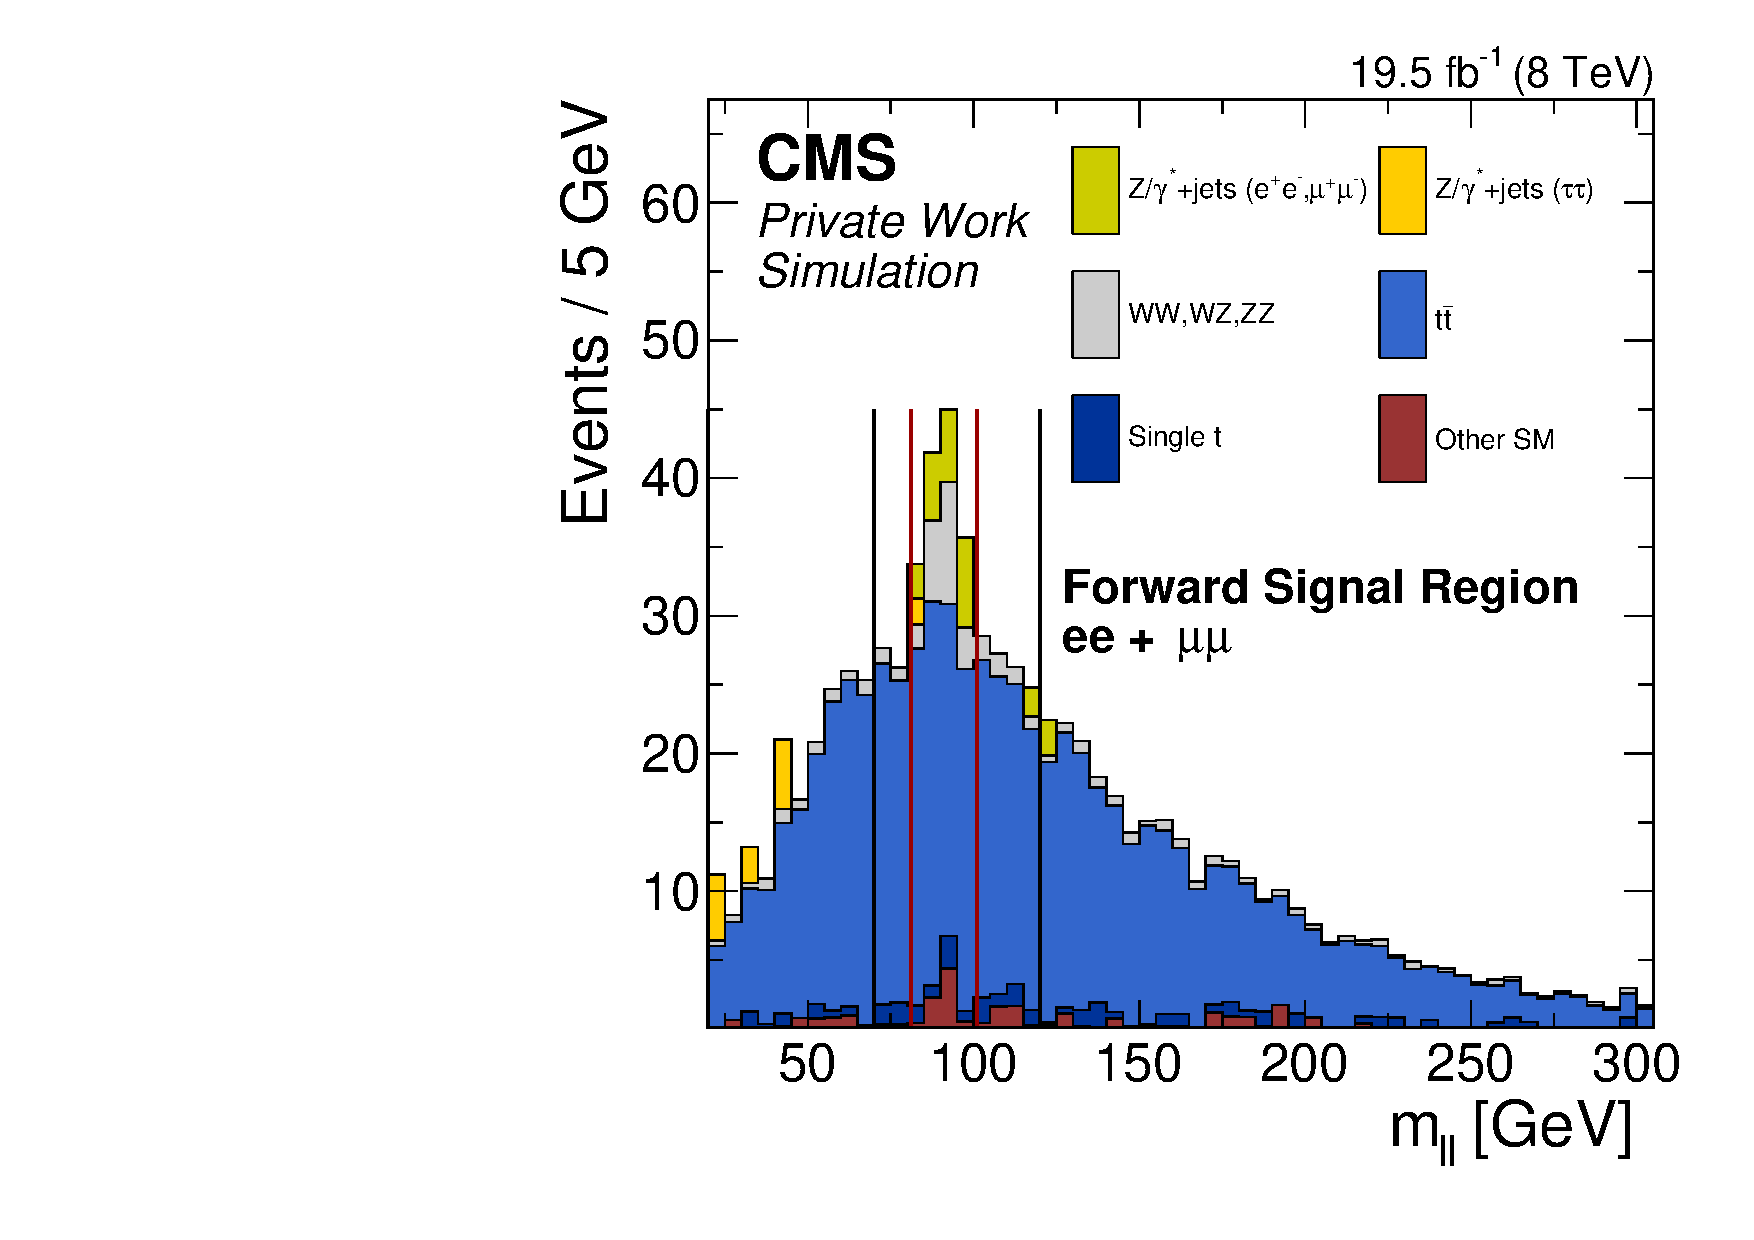
\includegraphics[width=\textwidth]{plots/SELECTION/SignalForward_Mll_Full2012_SF_TopReweighted_MCOnly.pdf}
\end{minipage}
\caption{Distribution of \mll in SM simulation in the signal regions. The different background contributions are shown as stacked histograms. The distribution is normalised to \lumi. The red lines indicate the on-\Z region while the black lines show the boundaries of the low-mass and high-mass regions.}
\label{fig:sigMC}
\end{figure}

For the shape analysis searching for edges in the \mll spectrum, the mass range $\mathrm{20}< \mll < \unit{300}{\giga\electronvolt}$ is studied. It is described in Section~\ref{sec:fit}.

\begin{table}[htb]
\centering
\caption{Summary of event selections applied in the analysis. Each of the selections in \njets and \MET (Drell--Yan control region, flavour-symmetric control region, and signal region) are applied on top of the inclusive dilepton selection. Selections in \mll and lepton $|\eta|$ are applied to select subsets of these regions.}
\label{tab:selections}
\begin{tabular}{l|c}
   &  selection  \\ \hline
  \multirow{5}{*}{inclusive dilepton selection} & event cleaning \\   
 &two isolated opposite-sign leptons \\ 
 & lepton $\unit{\pt > 20 }{\giga\electronvolt}$ \\
 &  $\Delta R(\ell\ell) > 0.3$ \\
 & $\mll > \unit{20}{\giga\electronvolt}$ \\
 & lepton $\abs{\eta} < 2.4$ excl. $1.4 < \abs{\eta} < 1.6$ \\ \hline
  \multirow{3}{*}{Drell--Yan control region} & inclusive dilepton selection \\
	&  $\njets = 2$ \\
	& $\MET < \unit{50}{\giga\electronvolt}$ \\ \hline
	\multirow{3}{*}{Flav.-sym. control region} & inclusive dilepton selection \\	
	&  $\njets \geq 2$ \\
	& $\unit{50}{\giga\electronvolt} < \MET < \unit{100}{\giga\electronvolt}$ \\ \hline
	\multirow{4}{*}{Signal region} & inclusive dilepton selection \\	
	&  $\njets \geq 2$  and $\MET > \unit{150}{\giga\electronvolt}$ \\
	& or \\
	&  $\njets \geq 3$  and $\MET > \unit{100}{\giga\electronvolt}$ \\
	\hline
	\multicolumn{2}{c}{sub selections based on lepton kinematics} \\ \hline
 \multirow{4}{*}{\mll} & low-mass: $\mathrm{20}< \mll < \unit{70}{\giga\electronvolt}$ \\ 	
 & on-Z: $\mathrm{80}< \mll < \unit{101}{\giga\electronvolt}$ \\
 & high-mass: $\unit{120}{\giga\electronvolt} < \mll$ \\
 & fit: $\mathrm{20}< \mll < \unit{300}{\giga\electronvolt}$ \\ \hline
 \multirow{2}{*}{$\abs{\eta}$} & central: both $\abs{\eta} < 1.4$\\ 	
 & forward: at least one $\abs{\eta} > 1.6$ \\ 
\end{tabular}
\end{table}
\chapter{Estimation of Standard Model backgrounds}
\label{sec:backgrounds}
Different SM processes contribute to the event sample in the signal region, as indicated for example in Figure~\ref{fig:sigRegionBG}. To distinguish a potential signal from these backgrounds, a precise estimation of the background contributions is essential. While the simulation of these processes and the response of the CMS detector gives a good description of the data for the majority of the phase space, a large number of uncertainty sources are introduced in the modelling of the physical processes and the detector. Therefore, a higher precision can be achieved by deriving the background estimates directly from the recorded data. Dedicated methods are applied for the flavour-symmetric and Drell--Yan backgrounds (see Section~\ref{sec:SMBackgrounds}). The results of these methods are used directly in the counting experiment (see Section~\ref{sec:counting}). The fit in search for a kinematic edge performs shape based estimates of the SM backgrounds. However, the results of the studies of flavour-symmetry described below are used to constrain these backgrounds in the fit procedure.

\section{Flavour-symmetric backgrounds}
Processes that are symmetric in the production of SF and OF lepton pairs allow for the estimation of their contribution to the SF event sample from the OF yield. The relevant backgrounds contributing to this class have been discussed in Section~\ref{sec:SMBackgrounds}. Additional contributions are coming from misidentified leptons, as will be demonstrated later. 

No significant deviation from flavour-symmetry has been observed in the decays of the \W boson, with a measured ratio of the branching fractions into $e+\nu$ and $\mu + \nu$ of $\frac{BF(\W\rightarrow e\nu)}{BF(\W\rightarrow \mu\nu)} = 1.007\pm0.021$~\cite{PDG}. In the decays of the $\tau$ lepton the different masses of electron and muon have a small, but noticeable effect, resulting in a slightly favoured decay into electrons with ratio of branching fractions of  $\frac{BF(\tau\rightarrow e\nu)}{BF(\tau\rightarrow \mu\nu)} = 1.0241\pm0.0032$~\cite{PDG}. As backgrounds with $\tau$ leptons are a sub-dominant contribution to the flavour-symmetric background, these can be considered to be fully flavour-symmetric on particle level. 

However, deviations from flavour-symmetry are introduced by the different efficiencies for triggering, reconstructing, and identifying electrons and muons in CMS. The background estimation from OF events $N_{SF}^{pred}$, therefore, has to include a correction for this deviation, which is applied as a multiplicative factor to the observed OF event yield $N_{OF}$:
\begin{equation*}
N_{SF}^{\text{pred}} = \Rsfof \cdot N_{OF}.
\end{equation*}
Similarly, the factors \Reeof and \Rmmof are used to derive separate background estimates for the \EE and \MM channels. Two independent methods are utilised to measure \Rsfof on data. In the first approach the ratio is directly measured as the ratio of SF to OF events in the control region for flavour-symmetric backgrounds (see Table~\ref{tab:selections}). The second approach studies the lepton efficiencies and derives \Rsfof factorised into the effects of trigger efficiencies and reconstruction and identification efficiencies. 

\subsection{Direct measurement of \Rsfof}
The ratio \Rsfof is calculated in the control region for flavour-symmetric backgrounds. As an initial step, possible dependencies of \Rsfof are studied in simulation, as the statistical uncertainties are lower compared to the data. The ratio of SF to OF events in the flavour-symmetric control region as a function of \mll in simulation is shown in Figure~\ref{fig:controlRatioMC}, separately for the central and forward lepton selection. The ratio is very close to one and independent of \mll, except at the \Z boson peak, where a significant Drell--Yan contribution spoils the SF-OF symmetry. It can be concluded that an universal factor can be applied for flavour-symmetric backgrounds over the full mass range. To exclude the \Z boson peak from the calculation only events in the mass regions $\unit{20}{\giga\electronvolt}< \mll < \unit{70}{\giga\electronvolt}$ and $\mll > \unit{120}{\giga\electronvolt}$ are considered.   	
\begin{figure}
\begin{center}
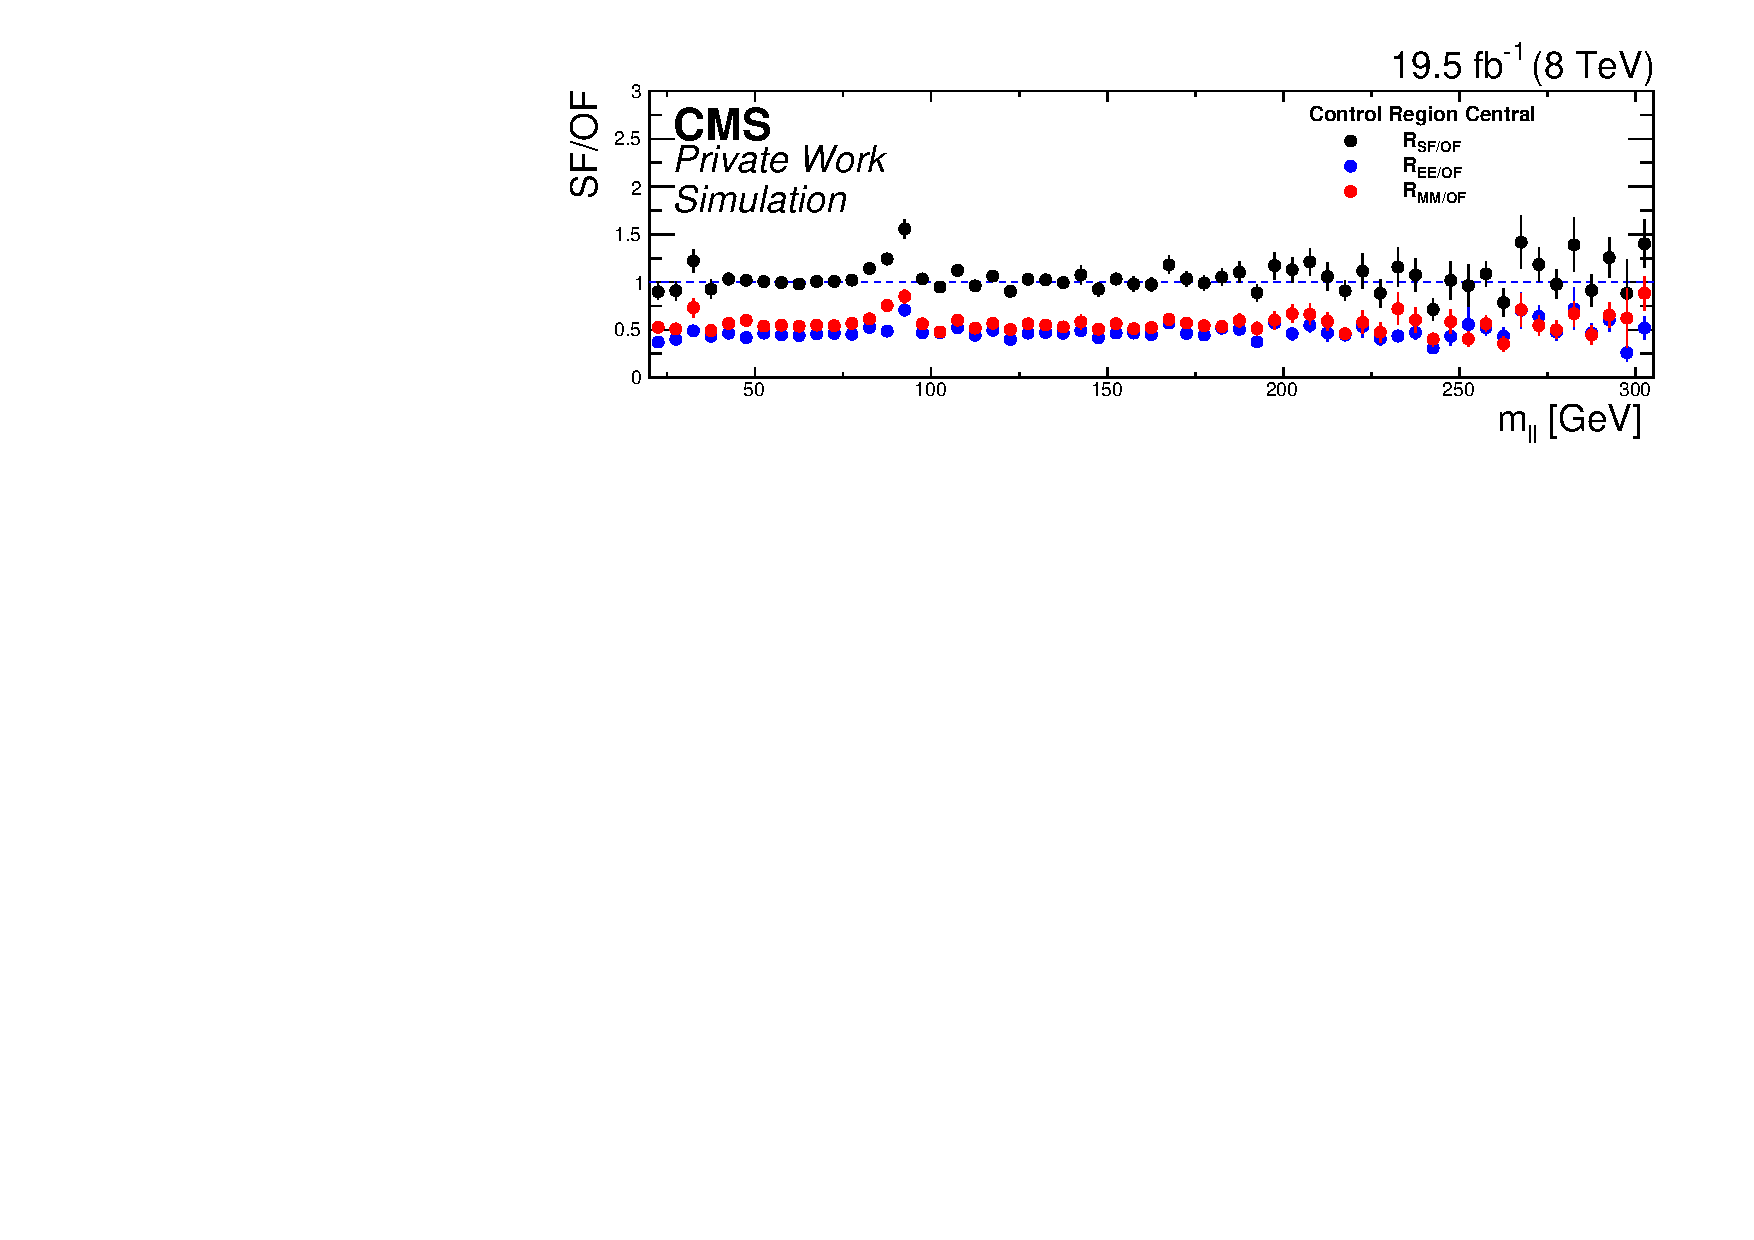
\includegraphics[scale=0.5]{plots/BG/control/rSFOF_ControlCentral_Full2012_Mll_None_MC.pdf}\\
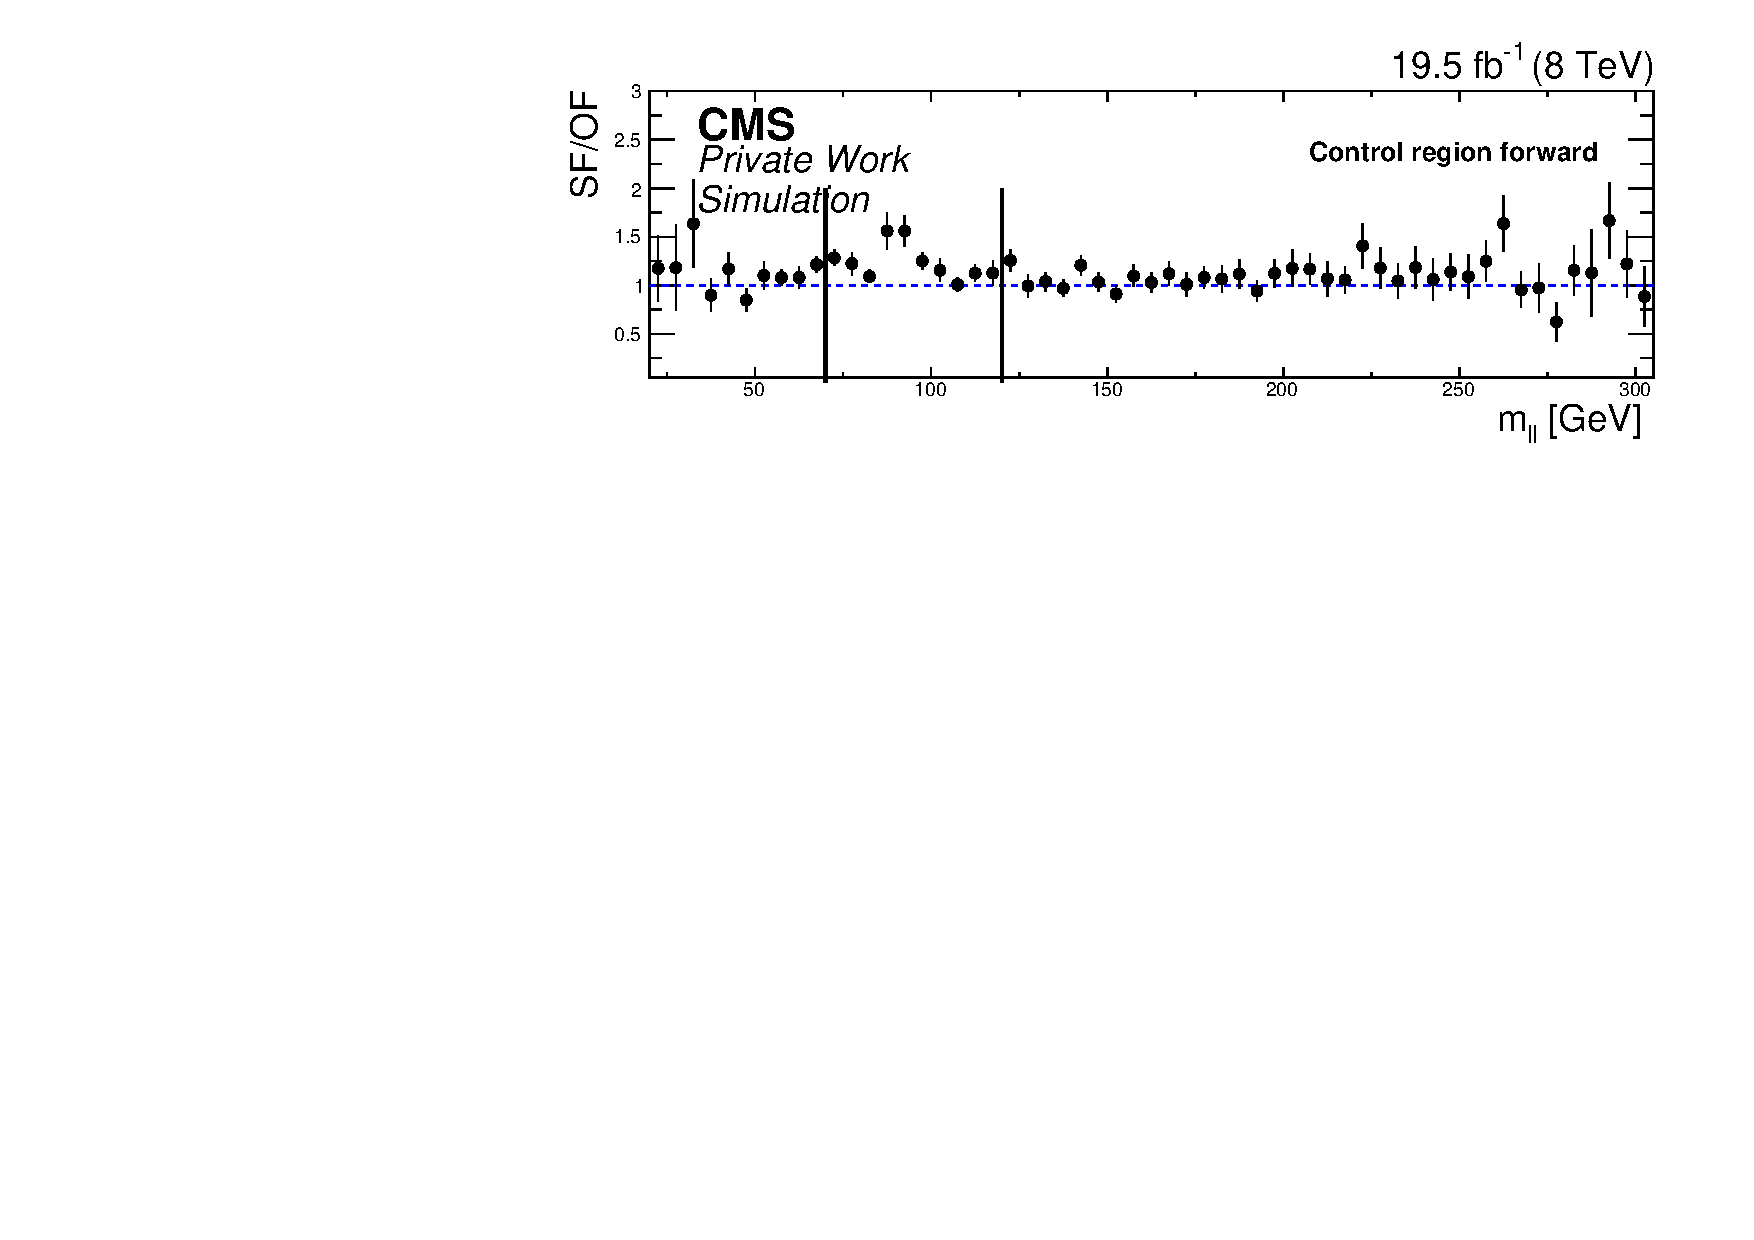
\includegraphics[scale=0.5]{plots/BG/control/rSFOF_ControlForward_Full2012_Mll_None_MC.pdf}
\caption{Ratio of SF to OF events as a function of \mll in the flavour-symmetric control region in simulation. All contributing background processes have been considered. Shown are the results for the central (top) and forward (bottom) lepton selection. The black vertical lines indicate the upper boundary of the low-mass region and the lower boundary of the high-mass region.}
\label{fig:controlRatioMC}
\end{center}
\end{figure}

The observed ratio in data as a functions of \mll is shown in Figure~\ref{fig:controlRatio}. As expected from the simulation, no significant dependence on \mll is observed both in the central and forward signal lepton selection.
\begin{figure}
\begin{center}
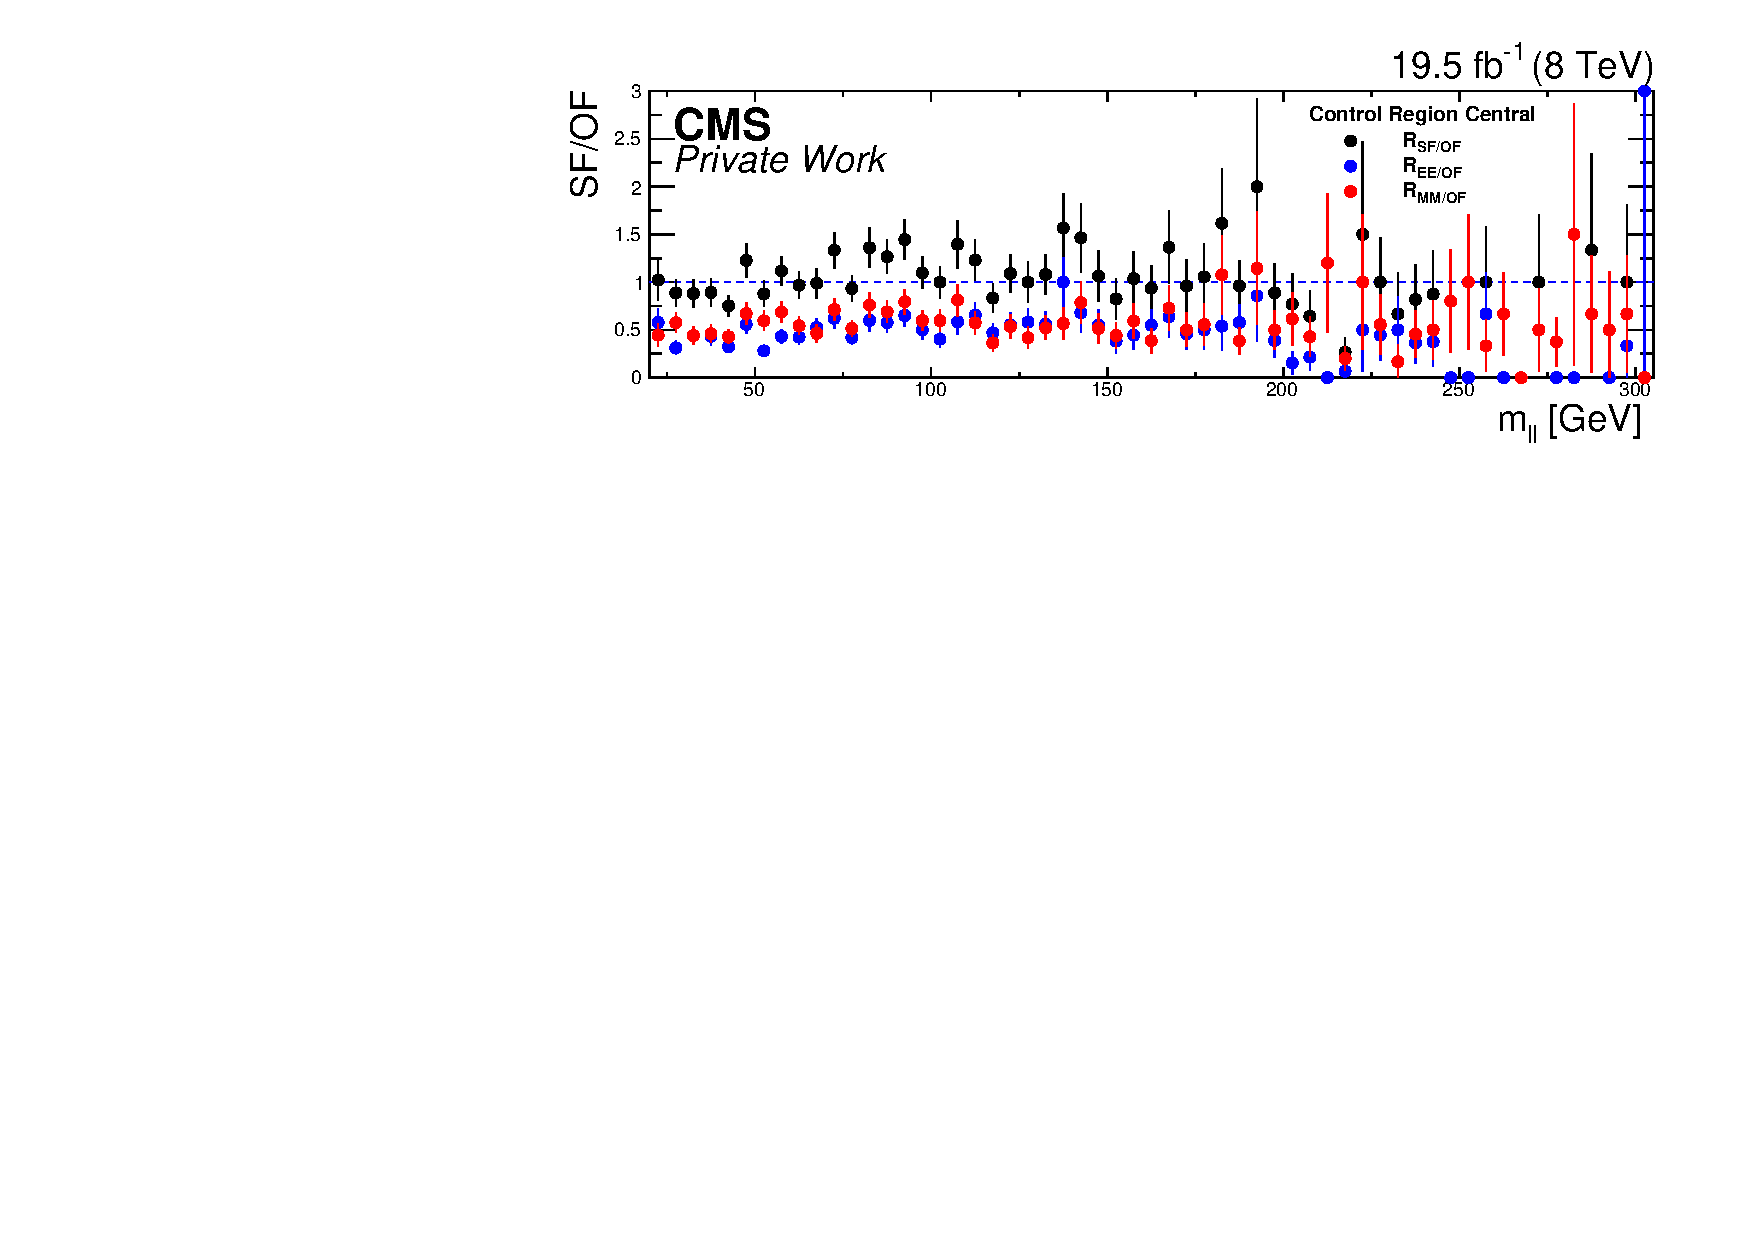
\includegraphics[scale=0.5]{plots/BG/control/rSFOF_ControlCentral_Full2012_Mll_None.pdf}\\
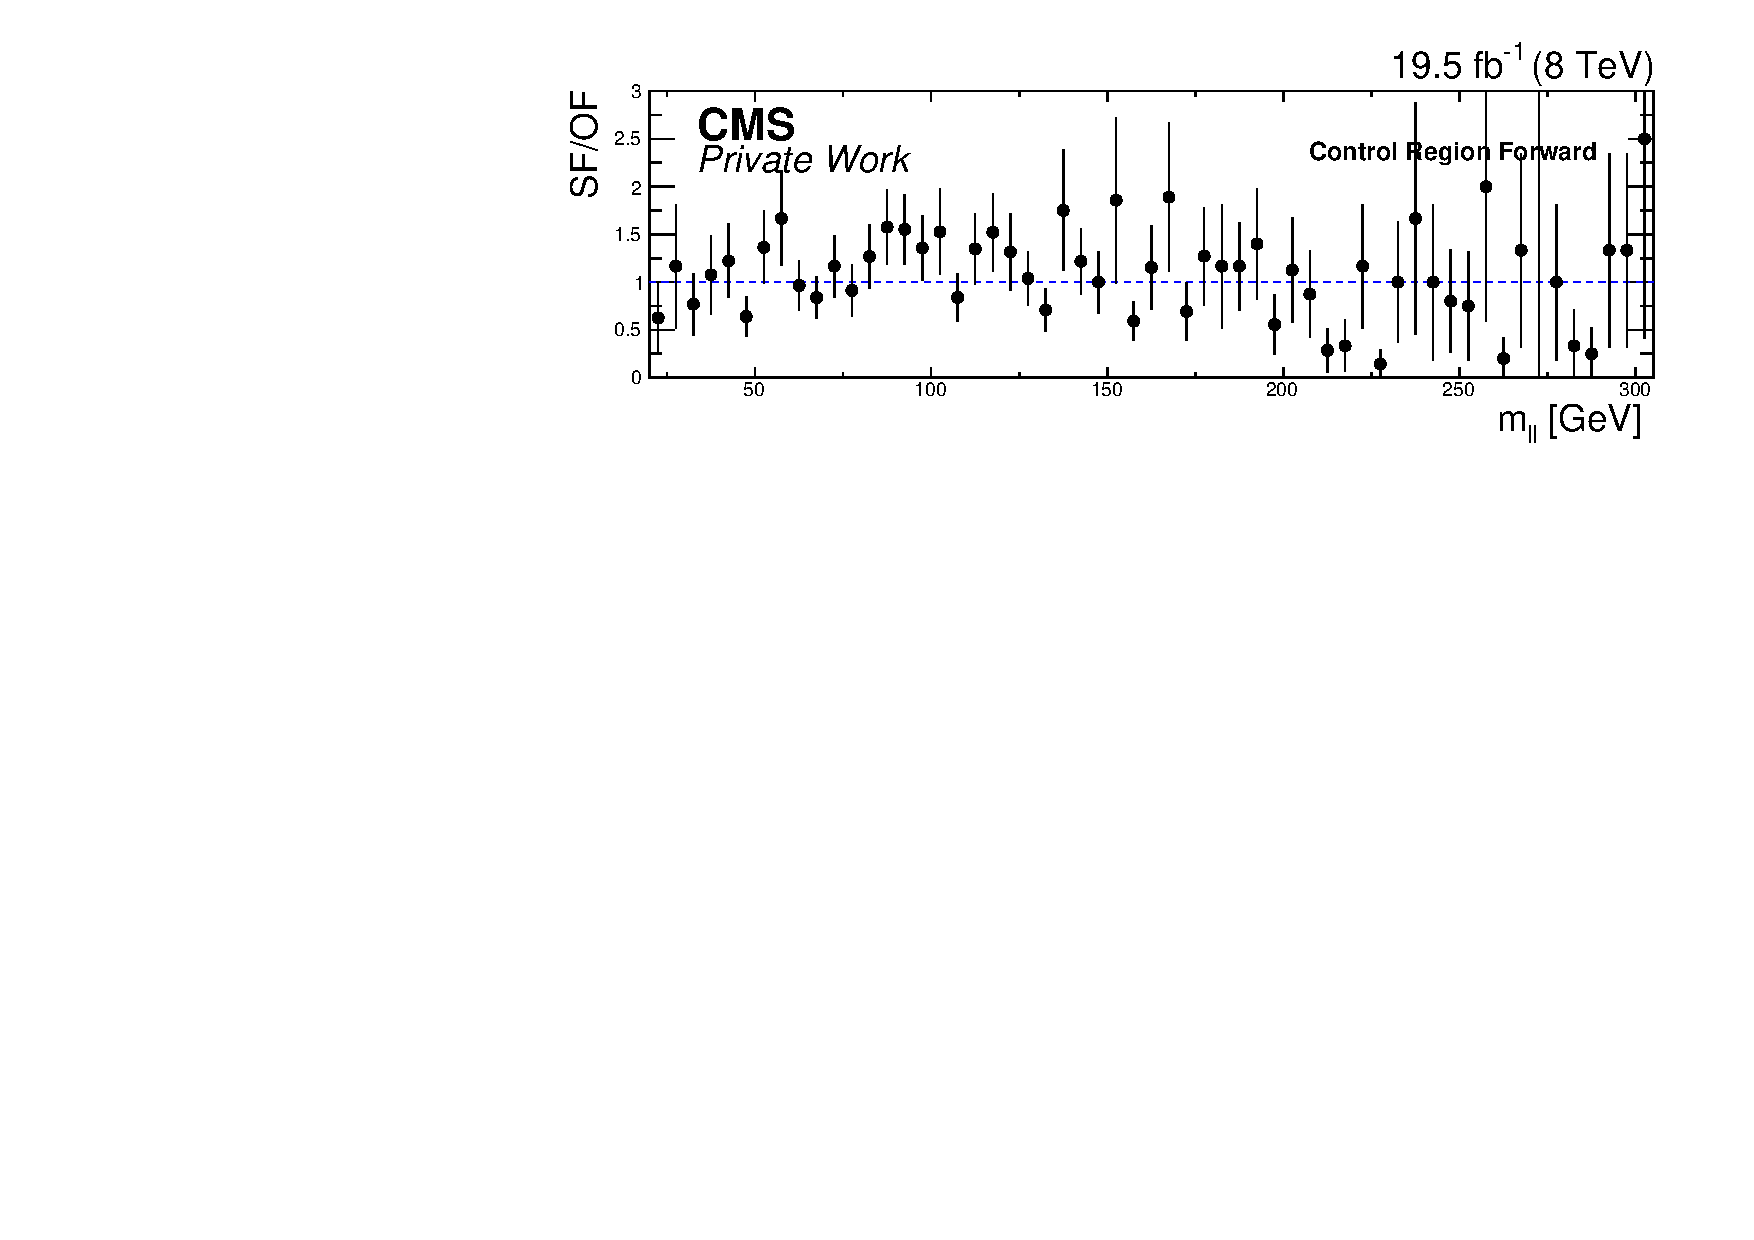
\includegraphics[scale=0.5]{plots/BG/control/rSFOF_ControlForward_Full2012_Mll_None.pdf}
\caption{Ratio of SF to OF events as a function of \mll in the flavour-symmetric control region in data. Shown are the results for the central (top) and forward (bottom) lepton selection. The black vertical lines indicate the upper boundary of the low-mass region and the lower boundary of the high-mass region.}
\label{fig:controlRatio}
\end{center}
\end{figure}
The numerical results are summarised in Table~\ref{tab:rSFOF} for \Rsfof as well as for \Reeof and \Rmmof. Agreement between the values measured in data and simulation is observed within the statistical uncertainties. The observed values in data are $\Rsfof = 1.007\pm0.037$ for the central and $1.015\pm0.062$ for the forward dilepton selection. 

The extrapolation of the measured value of \Rsfof into the signal region is tested in simulation by calculating the ratio of \Rsfof observed in the signal region to that in the control region. No deviation of the values measured in the signal region from those obtained in the control region is observed within the statistical uncertainties of the simulation. This statistical uncertainty of 0.020 for the central and 0.034 for the forward dilepton selection is therefore assigned as a systematic uncertainty of the method. 


\begin{table}[hbtp]
 \renewcommand{\arraystretch}{1.3}
 \setlength{\belowcaptionskip}{6pt}
 \centering
 \caption{Observed event yields in the control region and the resulting values of \Rsfof, \Reeof, and \Rmmof. The results are shown separately for the central and forward lepton selection and the same quantities derived on simulation are shown for comparison. For the simulation, the ratio between the values of \Rsfof, \Reeof, and \Rmmof measured in the signal and control region is shown.}
  \label{tab:rSFOF}
\begin{tabular}{l|c|c|c|c}
\multicolumn{5}{c}{Control region}\\ \hline     
 & $N_{SF}$ & $N_{OF}$ & $ \Rsfof \pm \sigma_{stat}$ & signal/control region $\pm \sigma_{stat}$  \\    
\hline
&  \multicolumn{4}{c}{Central} \\
\hline
 Data & 1458 & 1448 & 1.007$\pm$0.037 & -- \\
 MC & 1484.2 & 1436.1 & 1.034$\pm$0.015 & 1.016$\pm$0.020\\
 
 
    \hline 
& \multicolumn{4}{c}{Forward} \\
\hline
 Data & 545 & 537 & 1.015$\pm$0.062 & -- \\
 MC & 565.1 & 517.5 & 1.092$\pm$0.026 & 0.997$\pm$0.034\\

\hline\hline
 & $N_{ee}$ & $N_{OF}$ & $ \Reeof \pm \sigma_{stat}$ & signal/control region $\pm \sigma_{stat}$  \\    
\hline
&  \multicolumn{4}{c}{Central} \\
\hline
 Data & 663 & 1448 & 0.458$\pm$0.021 & -- \\
 MC & 670.0 & 1436.1 & 0.467$\pm$0.008 & 1.017$\pm$0.025\\
 
 
    \hline 
& \multicolumn{4}{c}{Forward} \\
\hline
 Data & 239 & 537 & 0.445$\pm$0.035 & -- \\
 MC & 237.9 & 517.5 & 0.460$\pm$0.014 & 1.023$\pm$0.043\\

\hline\hline
 & $N_{\mu\mu}$ & $N_{OF}$ & $ \Rmmof \pm \sigma_{stat}$ & signal/control region $\pm \sigma_{stat}$  \\    
\hline
& \multicolumn{4}{c}{Central} \\
\hline
 Data & 795 & 1448 & 0.549$\pm$0.024 & -- \\
 MC & 814.2 & 1436.1 & 0.567$\pm$0.010 & 1.015$\pm$0.025\\
 
 
    \hline 
 & \multicolumn{4}{c}{Forward} \\
\hline
 Data & 306 & 537 & 0.570$\pm$0.041 & -- \\
 MC & 327.3 & 517.5 & 0.632$\pm$0.018 & 0.978$\pm$0.039\\

  
\end{tabular}  
\end{table}


\subsection{Determination of \Rsfof with the factorisation method}
\label{sec:rmue}
Asymmetries between the lepton flavours introduced by differing reconstruction and selection efficiencies can be corrected for if the ratio of efficiencies for muons and electrons $\rmuestar = \frac{\epsilon_{\mu}}{\epsilon_{e}}$ is known. Here and in the following, the ``$^{*}$'' indicates that only reconstruction and selection efficiencies are considered in this definition. As all measurable quantities are affected by trigger efficiencies, these have to taken into account separately. The observable yield of OF events is therefore expressed as 
\begin{equation*}
N_{OF} = \epsilon_{e\mu}^T N_{OF}^{*},
\end{equation*}
where $\epsilon_{e\mu}^T$ is the efficiency of the $e\mu$ dilepton triggers. Similarly, \effeet and \effmmt denote the efficiencies of the dielectron and dimuon triggers.

Under the assumption that the efficiencies for the two leptons in the event have negligible correlation and the dilepton efficiency factorises, i.e. $\epsilon_{\ell\ell} = \epsilon_{\ell}\cdot\epsilon_{\ell}$, \rmuestar can be expressed in terms of the measured value \rmue, which is derived from the \EE and \MM event yields in the Drell-Yan control region (see Section~\ref{sec:rmue}) as 
\begin{equation*}
\rmue  = \sqrt{\frac{N_{\mu\mu}}{N_{ee}}} \approx \sqrt{\frac{\epsilon_{\mu}^2 \effmmt}{\epsilon_{e}^2 \effeet}} = \rmuestar \cdot \sqrt{\frac{\effmmt}{\effeet}}.
\end{equation*}

The predicted number of dielectron and dimuon events can be expressed in terms of the opposite-flavour yield using the relations
\begin{equation*}
\frac{1}{\epsilon_{ee}^T} N_{ee}^{\text{pred}} = \frac{1}{2}\cdot \frac{1}{\epsilon_{e\mu}^T} \frac{N_{OF}}{\rmuestar} = \frac{1}{2}\cdot \frac{1}{\rmue} \sqrt{\frac{\effmmt}{\effeet}} \frac{1}{\epsilon_{e\mu}^T} N_{OF}
\end{equation*}
and 
\begin{equation*}
\frac{1}{\epsilon_{\mu\mu}^T} N_{\mu\mu}^{\text{pred}} = \frac{1}{2} \cdot \rmuestar \frac{1}{\epsilon_{e\mu}^T} \cdot N_{OF} = \frac{1}{2} \cdot \rmue \sqrt{\frac{\effeet}{\effmmt}} \frac{1}{\effemt} \cdot N_{OF}.
\end{equation*}
The combined prediction for the same-flavour yield is therefore given by
\begin{equation*}
N_{SF}^{\text{pred}} = N_{ee}^{\text{pred}} + N_{\mu\mu}^{\text{pred}}.
\end{equation*}

In summary, the final expressions for the predicted yields in the same-flavour channels become
\begin{equation}
N_{ee}^{\text{pred}} = \frac{1}{2\rmue} \cdot \frac{\sqrt{\effeet \effmmt}}{\effemt} N_{OF} = \Reeof N_{OF}
\label{eq:nee}
\end{equation} 
and
\begin{equation}
N_{\mu\mu}^{\text{pred}} = \frac{1}{2}\rmue  \cdot \frac{\sqrt{\effeet \effmmt}}{\effemt} N_{OF} = \Rmmof N_{OF}.
\label{eq:nmm}
\end{equation} 
The combined prediction of the SF yield is, therefore:
\begin{equation}
N_{SF}^{\text{pred}} = \frac{1}{2}\left(\rmue + \frac{1}{\rmue}\right) \cdot \frac{\sqrt{\effeet \effmmt}}{\effemt}  N_{OF} = \Rsfof N_{OF}.
\label{eq:nsf}
\end{equation}
The factor containing the trigger efficiencies is abbreviated as
\begin{equation}
R_{\mathrm{T}} = \frac{\sqrt{\effeet \effmmt}}{\effemt}.
\label{eq:RT}
\end{equation}
\subsubsection{Measurement of $\mathbf{r_{\mu e}}$}
The measurement of \rmue is performed in the Drell-Yan control region (see Table~\ref{tab:selections}) as the ratio of \MM to \EE events on the Z boson peak, requiring $\unit{60}{\giga\electronvolt} < \mll < \unit{120}{\giga\electronvolt}$. A comparison of the recorded data to the different contributions  from SM processes, estimated from simulation, is shown in Figure~\ref{fig:rmueMll}. The Drell-Yan process is the dominating source of events in this selection. Good agreement between data and simulation is observed, indicating a good understanding of this kinematic region by the CMS simulation. Towards higher masses the data is underestimated by the simulation because mass-dependent higher order effects are not included in the simulation and result in a lack of events in the simulated samples.  
\begin{figure}[htbp]
\centering
\begin{minipage}[t]{0.49\textwidth}
  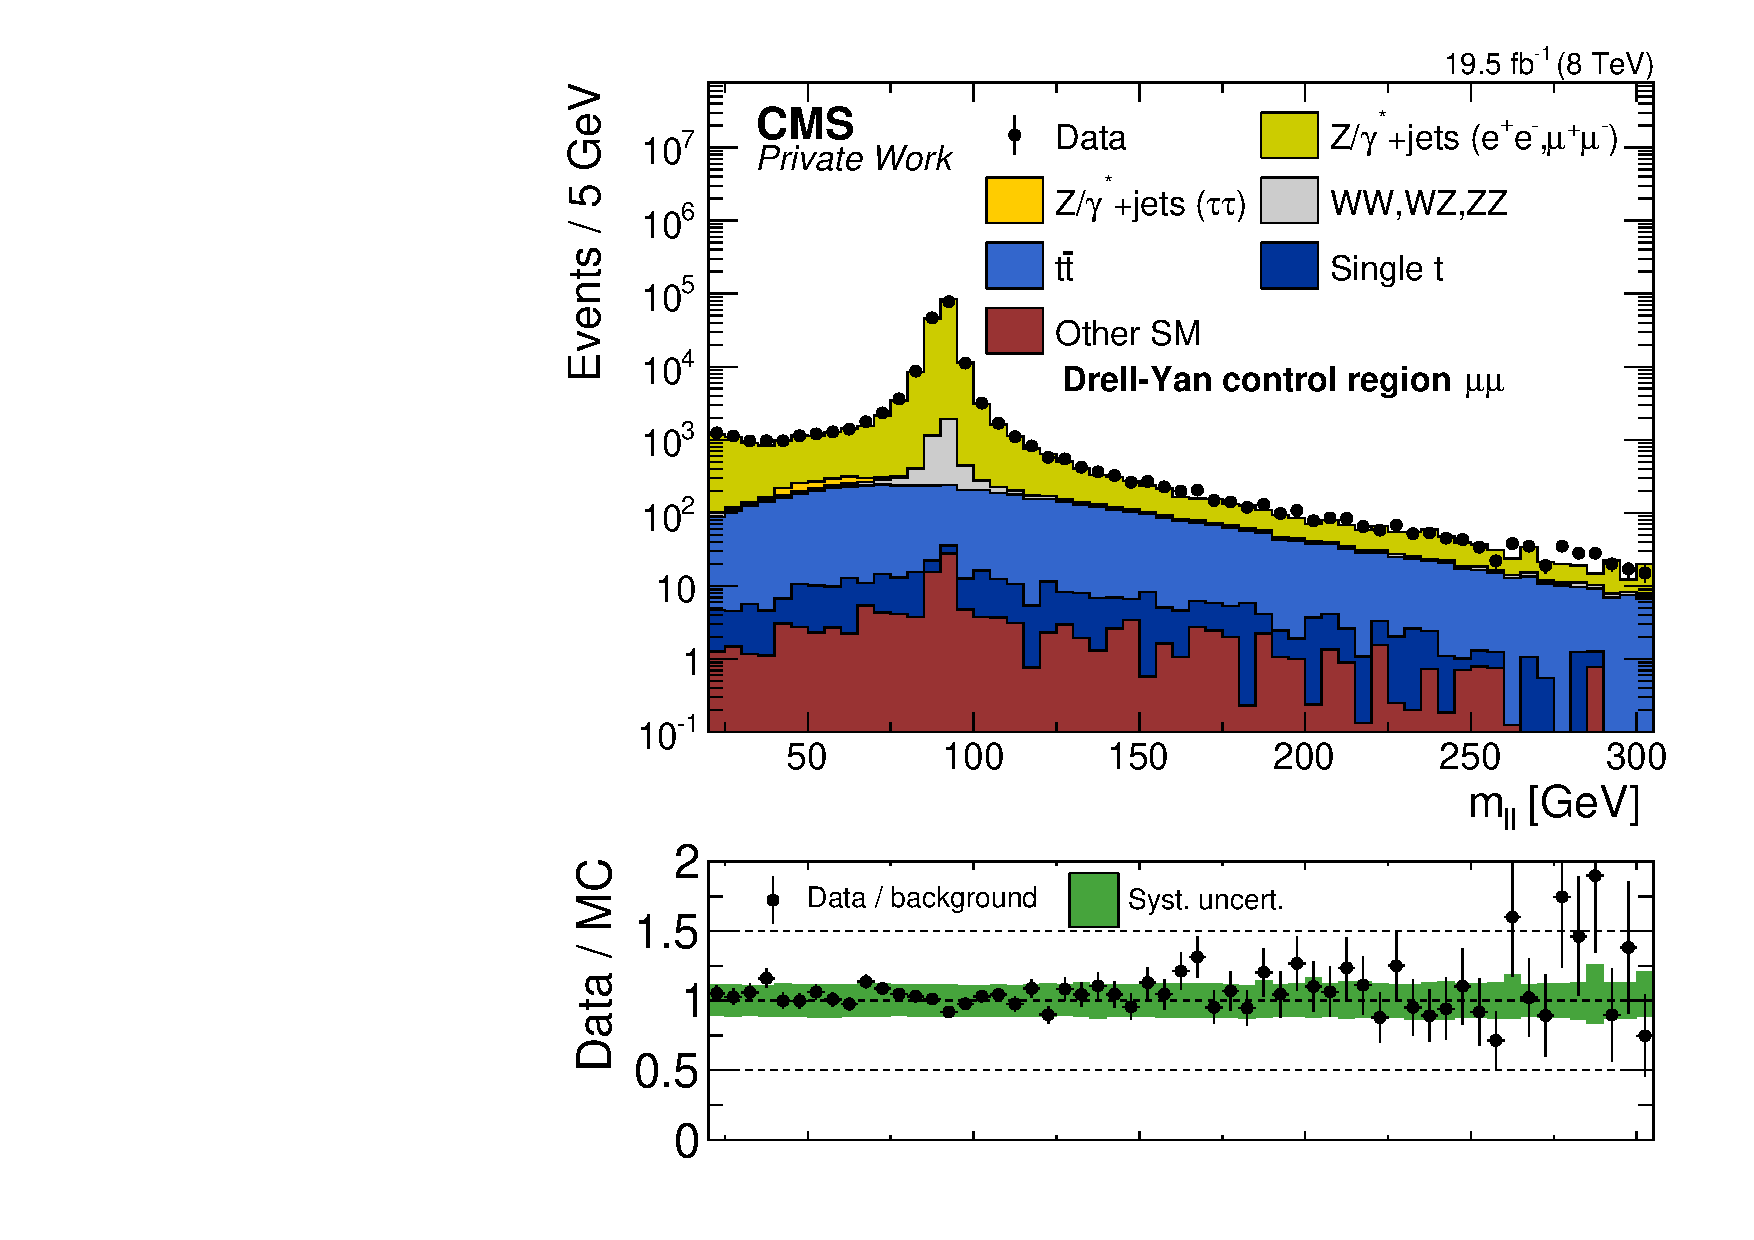
\includegraphics[width=\textwidth]{plots/BG/rmue/DrellYanControl_Mll_Full2012_MuMu_TopReweighted.pdf}
\end{minipage}
\begin{minipage}[t]{0.49\textwidth}
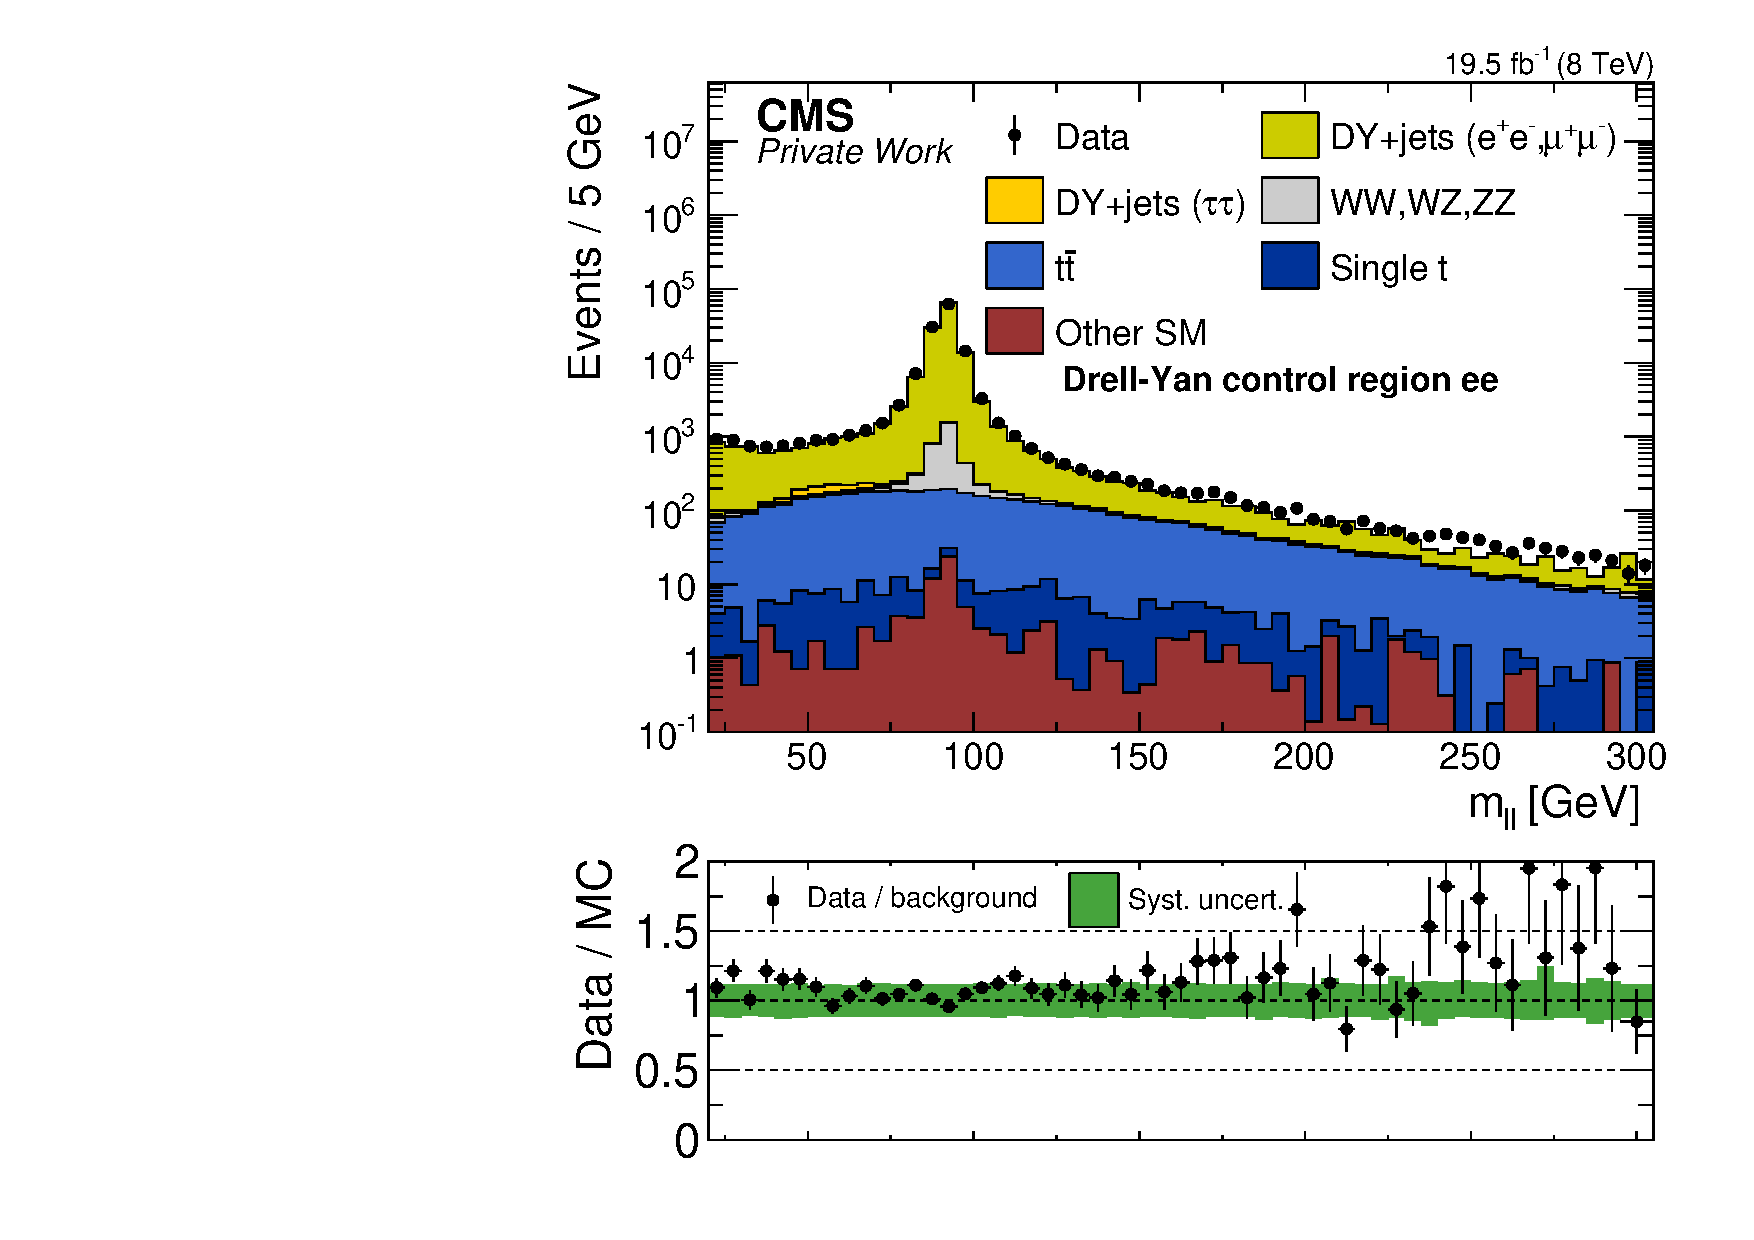
\includegraphics[width=\textwidth]{plots/BG/rmue/DrellYanControl_Mll_Full2012_EE_TopReweighted.pdf}
\end{minipage}
\caption{Distribution of \mll in the Drell-Yan control region for \MM events (left) and \EE events (right). The data is shown as the black dots, while the contributions from SM processes, estimated from simulation, are shown as the stacked histograms. The black lines indicate the region in \mll used in the measurement of \rmue.}
\label{fig:rmueMll}
\end{figure} 
The results of the calculation of \rmue are shown in Table~\ref{tab:rMuE}. Given are the observed yields for \MM and \EE events and the resulting value of \rmue with statistical and systematic uncertainties. In the central lepton selection, the \MM yield is about 18\% higher than the \EE yield. Similar results are observed on Drell-Yan simulation. For events with leptons in the forward region, a larger asymmetry between muons and electrons is observed, as expected since the harsher pileup environment in the detector endcaps has a stronger effect on the electron efficiencies. Here the \MM yield is about 40\% higher than the \EE yield. 

\begin{table}[hbtp]
 \renewcommand{\arraystretch}{1.3}
 \setlength{\belowcaptionskip}{6pt}
 \centering
 \caption{Result of the calculation of \rmue. Shown are the observed event yields in the Drell--Yan control region for the central and forward lepton selection in the \EE and \MM channels and the resulting values of 
\rmue. The same quantaties derived from simulation are shown for comparison.}
  \label{tab:rMuE}
  \begin{tabular}{l| ccc }

    							& $N_{\mu\mu}$ &  $N_{ee}$ & $\rmue \pm \sigma_{\text{stat.}} \pm \sigma_{\text{syst.}}$ \\ 
    
    \hline
    							& \multicolumn{3}{c}{Central}  \\ 

    \hline
        Data       &  98284                   & 83035              &  1.09$\pm$0.01$\pm$0.11    \\

        MC       &  99719                   & 82035              &  1.10$\pm$0.00$\pm$0.11    \\

\hline
    							& \multicolumn{3}{c}{Forward}  \\ 

    \hline
        Data       &  62212                   & 44437              &  1.18$\pm$0.01$\pm$0.24    \\

        MC       &  66327                   & 45541              &  1.21$\pm$0.00$\pm$0.24    \\

  \end{tabular}
\end{table}



The systematic uncertainties assigned to the measured values of \rmue are 10\% for the central and 20\% for the forward lepton selection. These values are obtained by studying the dependency of \rmue on relevant observables. These are on the one hand properties of the lepton pairs, while on the other hand event properties as the jet multiplicity and \MET are studied to ensure the applicability of \rmue in the signal region. The dependencies of \rmue on \mll, \MET, and \njets are shown in Figure~\ref{fig:rmueDependencies}. Some dependency is observed in the case of \mll, where the values are higher for low \mll below the \Z boson mass. This can be traced back to a dependency on the \pt of the leptons, where the efficiencies for muons have sharper turn-ons compared to electrons. In data, there is a strong effect visible around the \Z boson mass for forward leptons. This is caused by a systematic shift of the position of the \Z boson peak between electrons and muons and is not a general property of \rmue, as is evident from the comparison with $t\bar{t}$ simulation shown in the upper right of Figure~\ref{fig:rmueDependencies}. No strong dependencies can be observed for \MET and \njets within the statistical uncertainties. All observed deviations from the central values are covered by the systematic uncertainties assigned to the measurement. Further information on the dependency studies can be found in Appendix~\ref{app:rmue}.
\begin{figure}[htbp]
\centering
\begin{minipage}[t]{0.49\textwidth}
  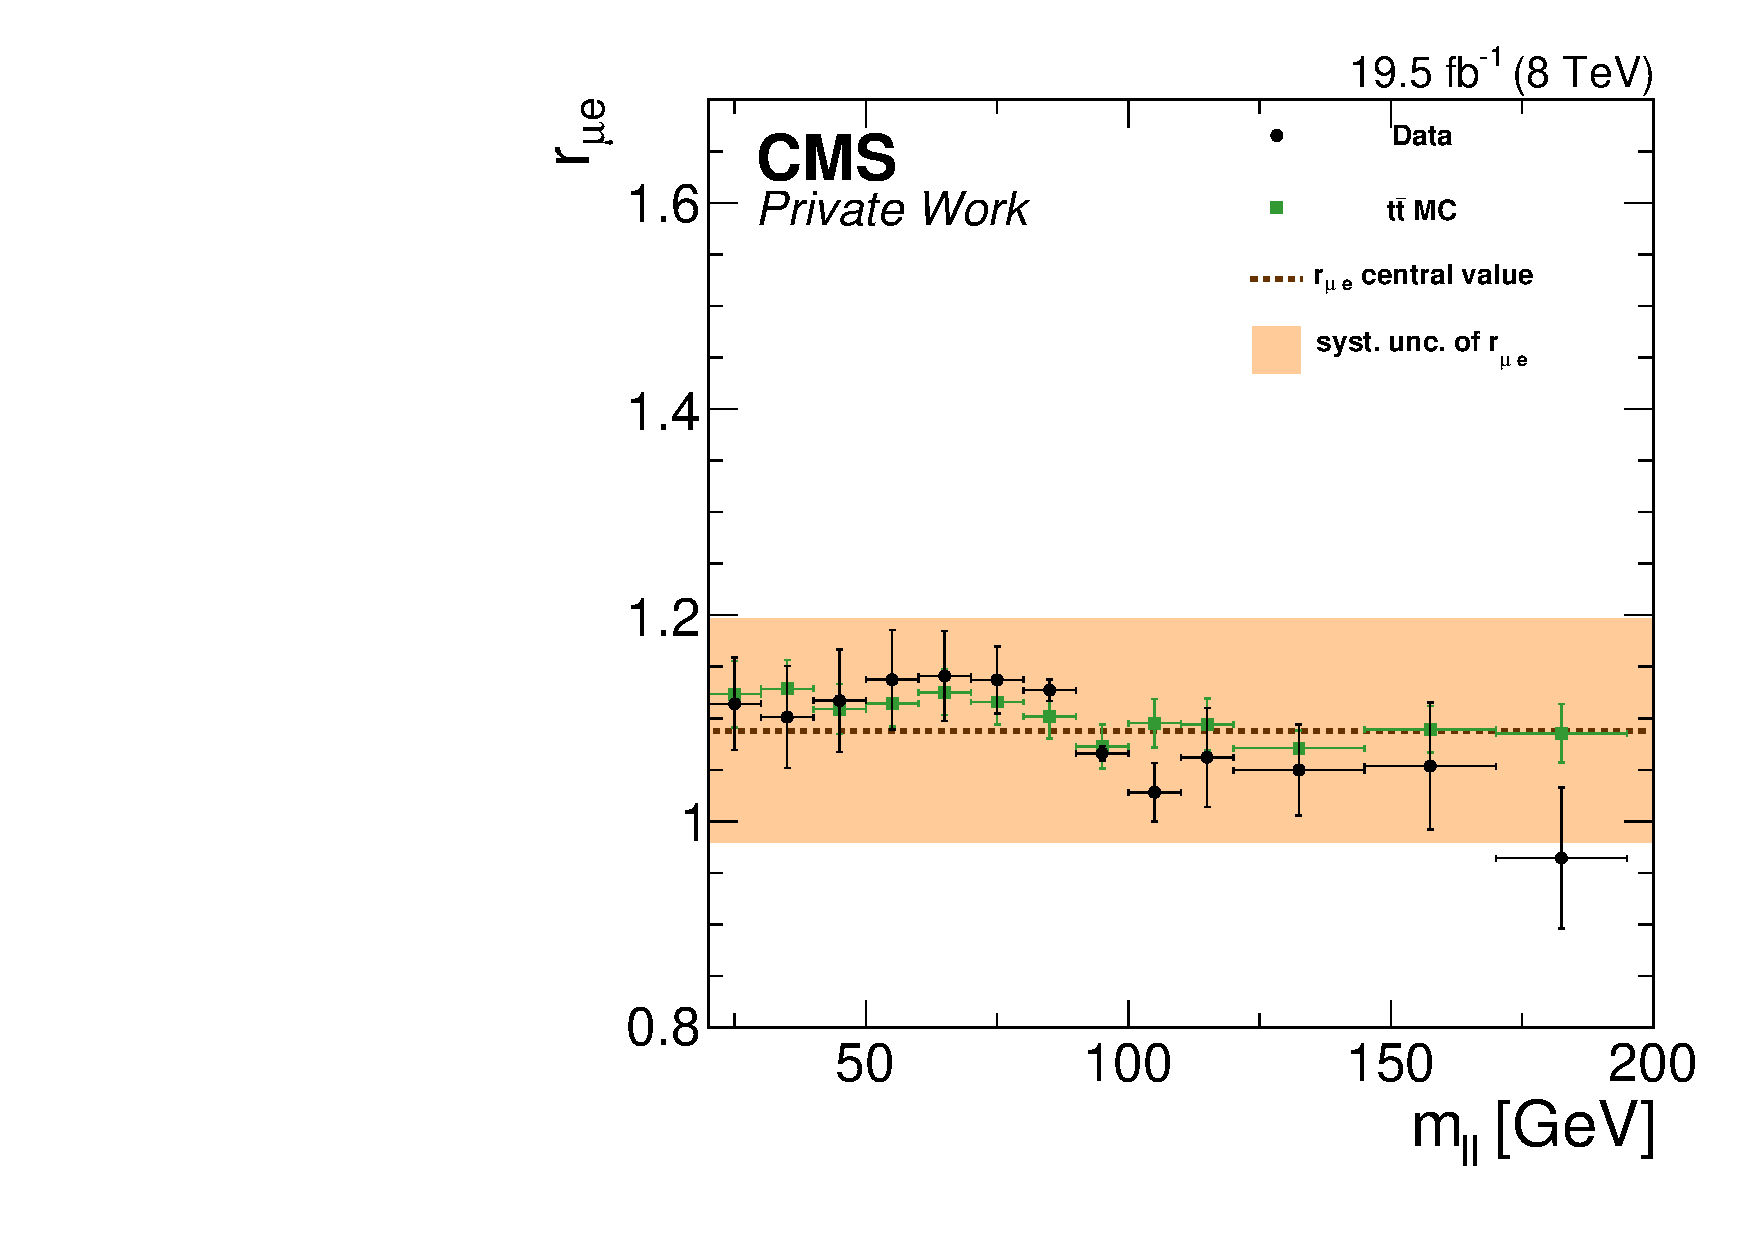
\includegraphics[width=\textwidth]{plots/BG/rmue/rMuE_ZPeakControlCentral_Full2012_Mll_None.pdf}
\end{minipage}
\begin{minipage}[t]{0.49\textwidth}
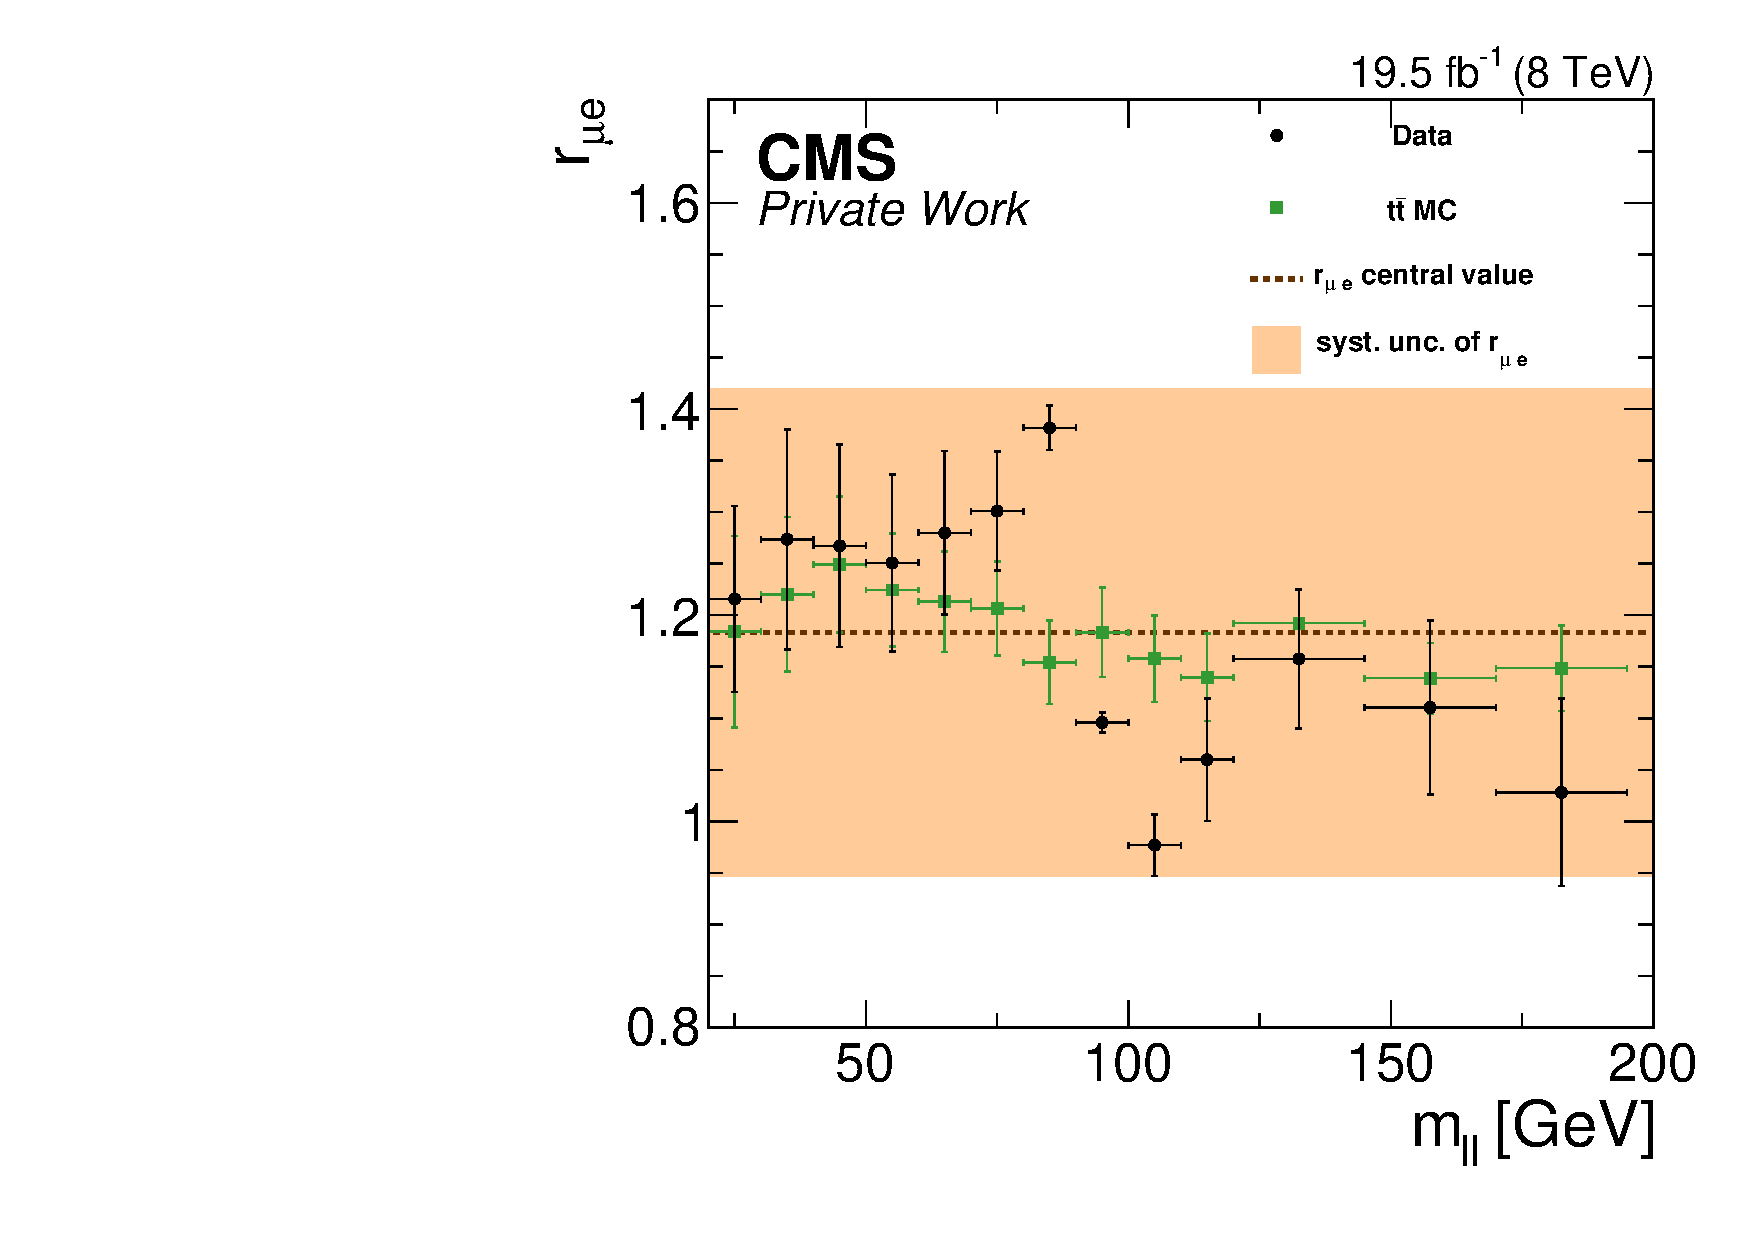
\includegraphics[width=\textwidth]{plots/BG/rmue/rMuE_ZPeakControlForward_Full2012_Mll_None.pdf}
\end{minipage}
\begin{minipage}[t]{0.49\textwidth}
  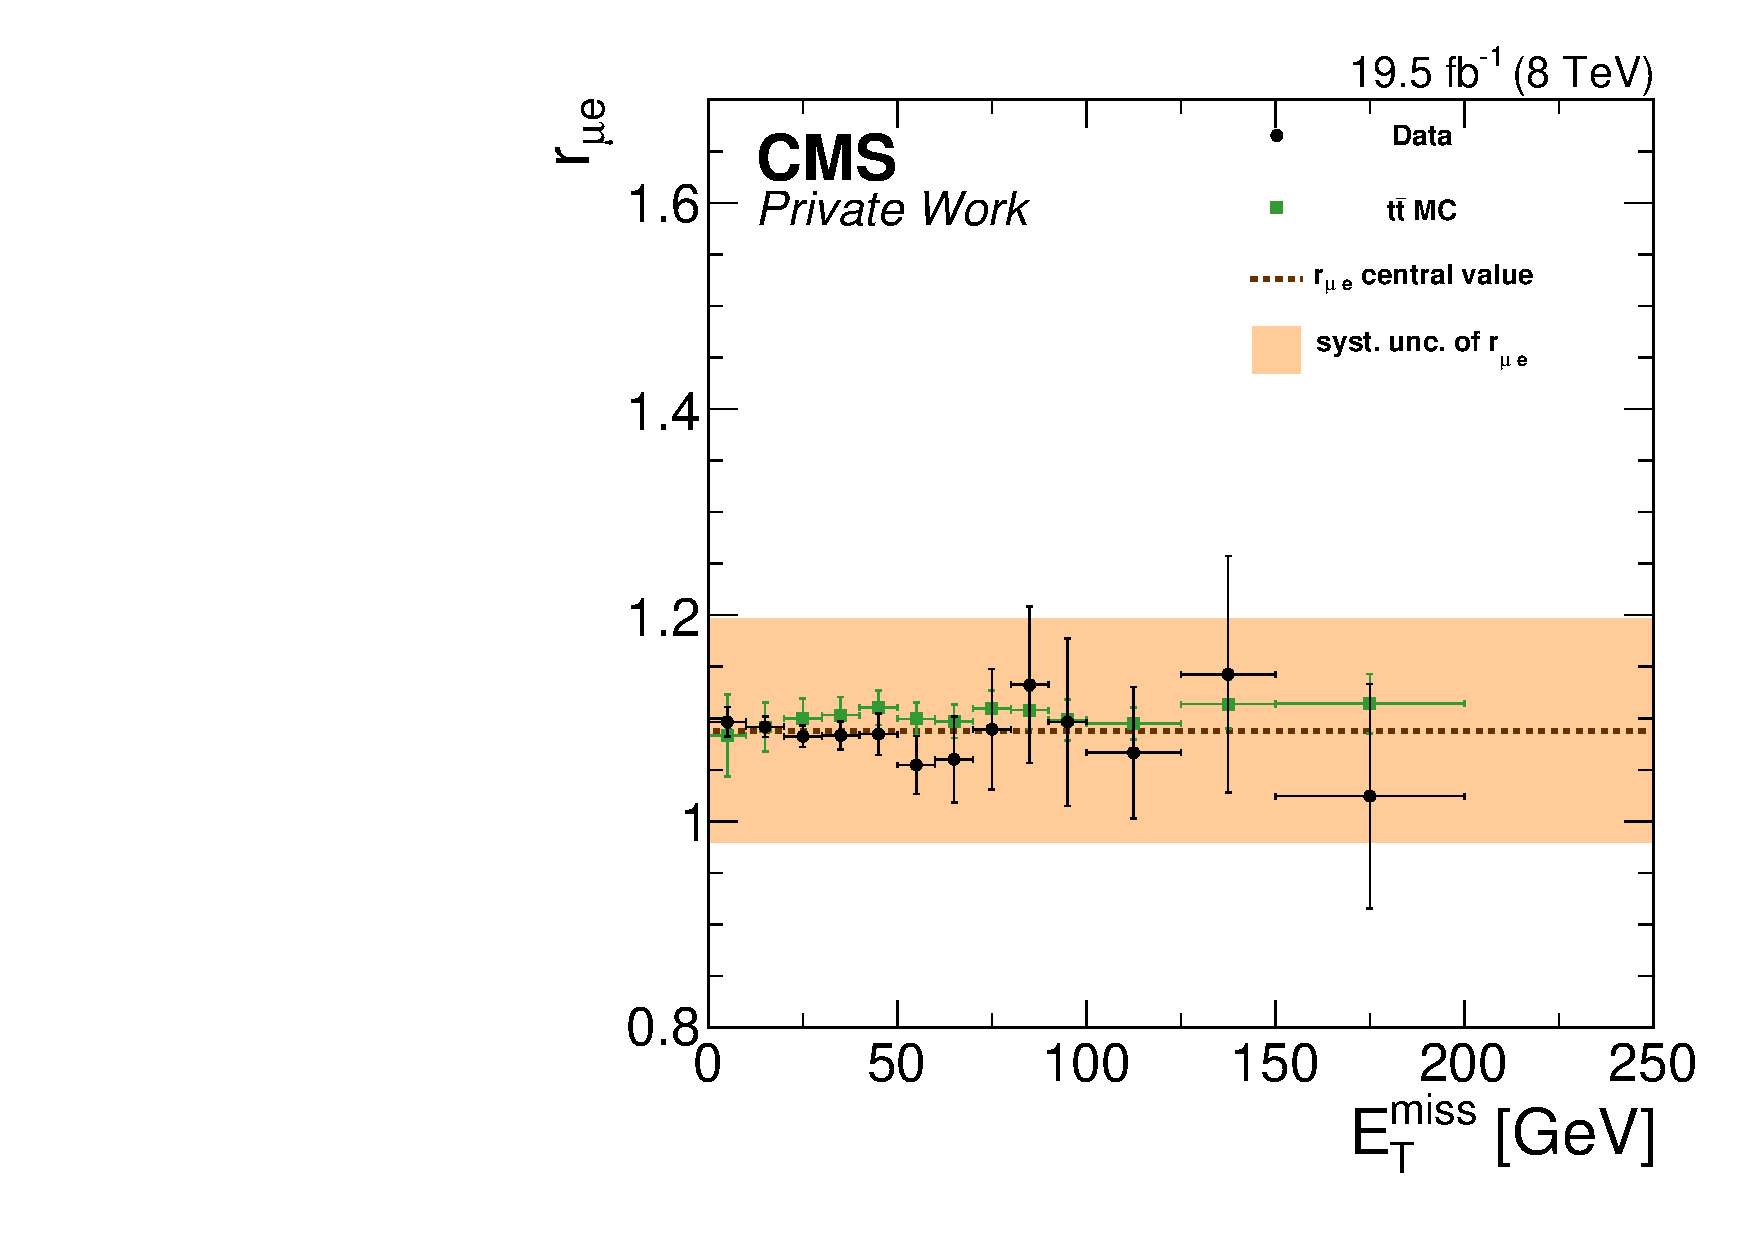
\includegraphics[width=\textwidth]{plots/BG/rmue/rMuE_ZPeakControlCentral_Full2012_MET_None.pdf}
\end{minipage}
\begin{minipage}[t]{0.49\textwidth}
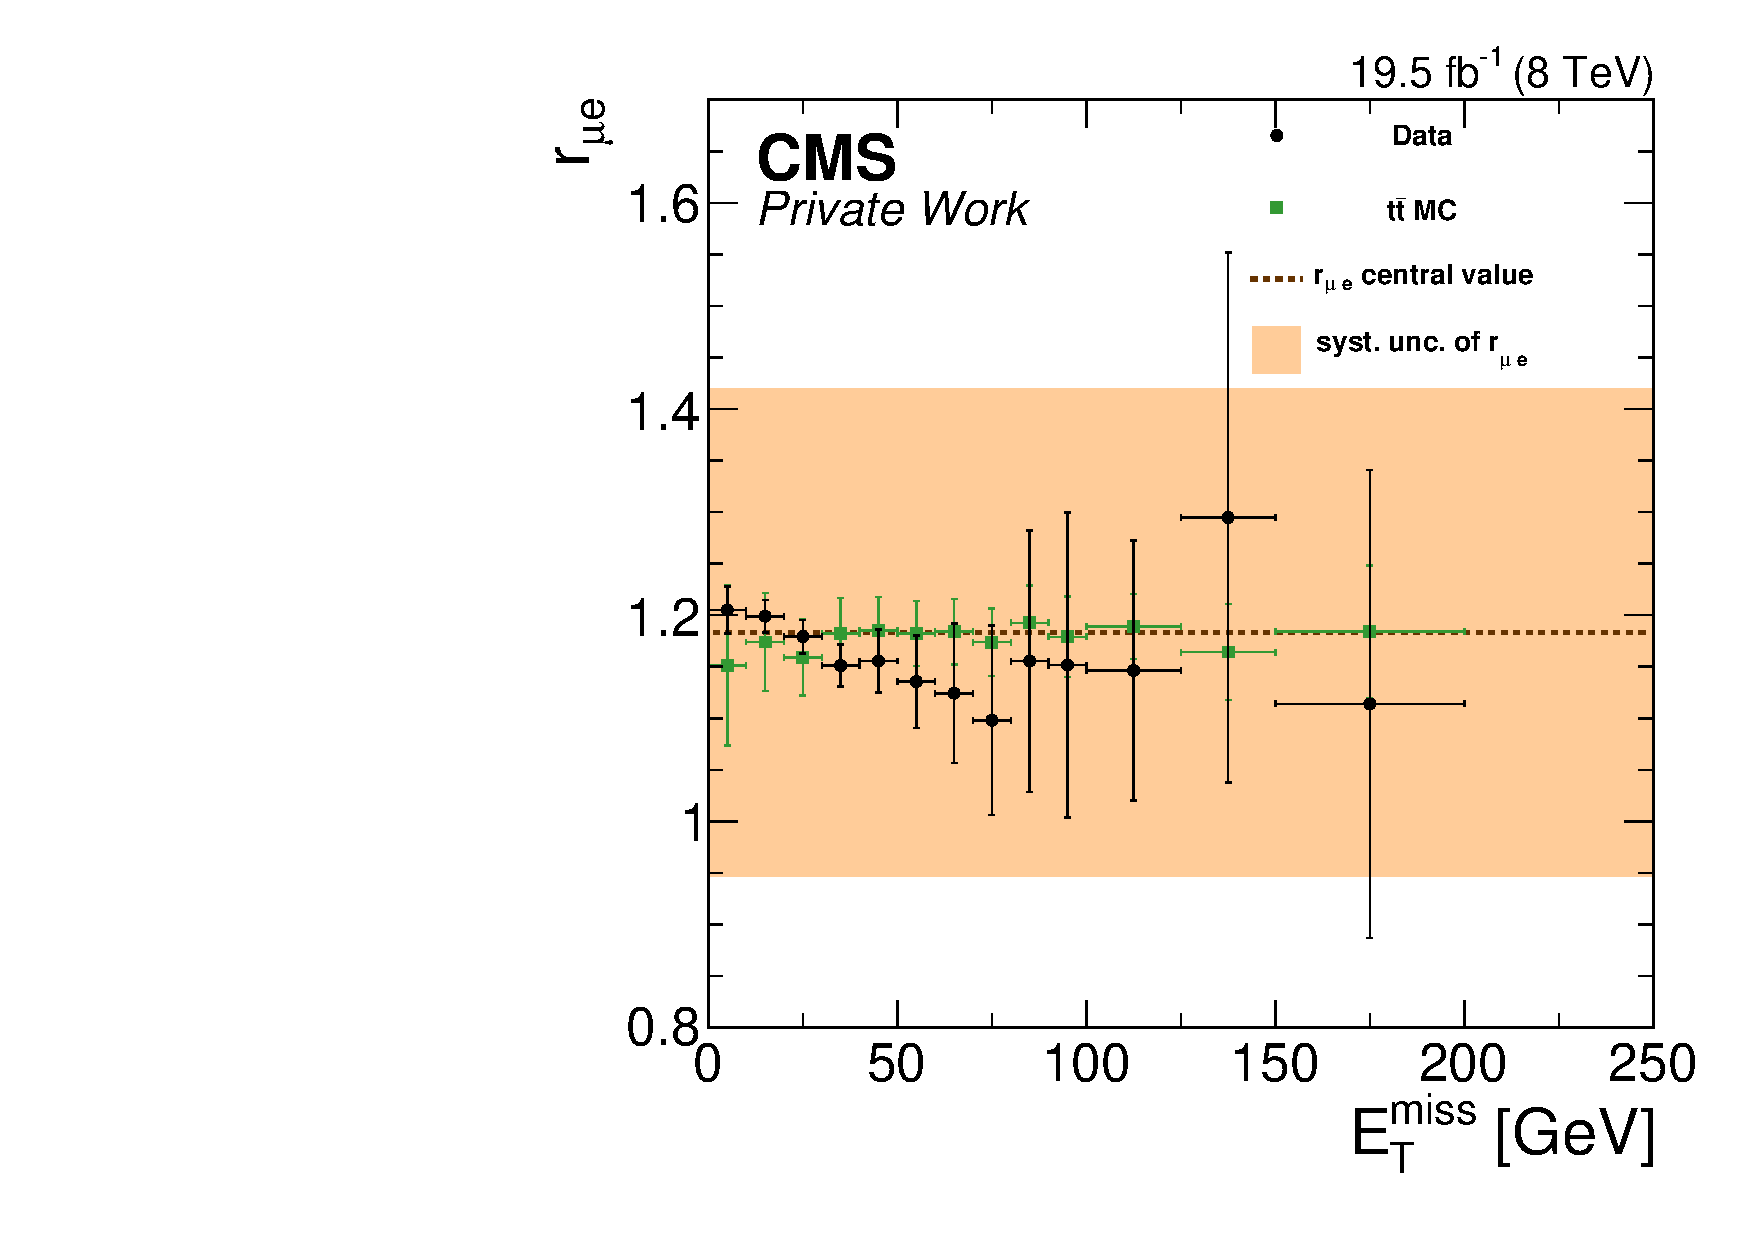
\includegraphics[width=\textwidth]{plots/BG/rmue/rMuE_ZPeakControlForward_Full2012_MET_None.pdf}
\end{minipage}
\begin{minipage}[t]{0.49\textwidth}
  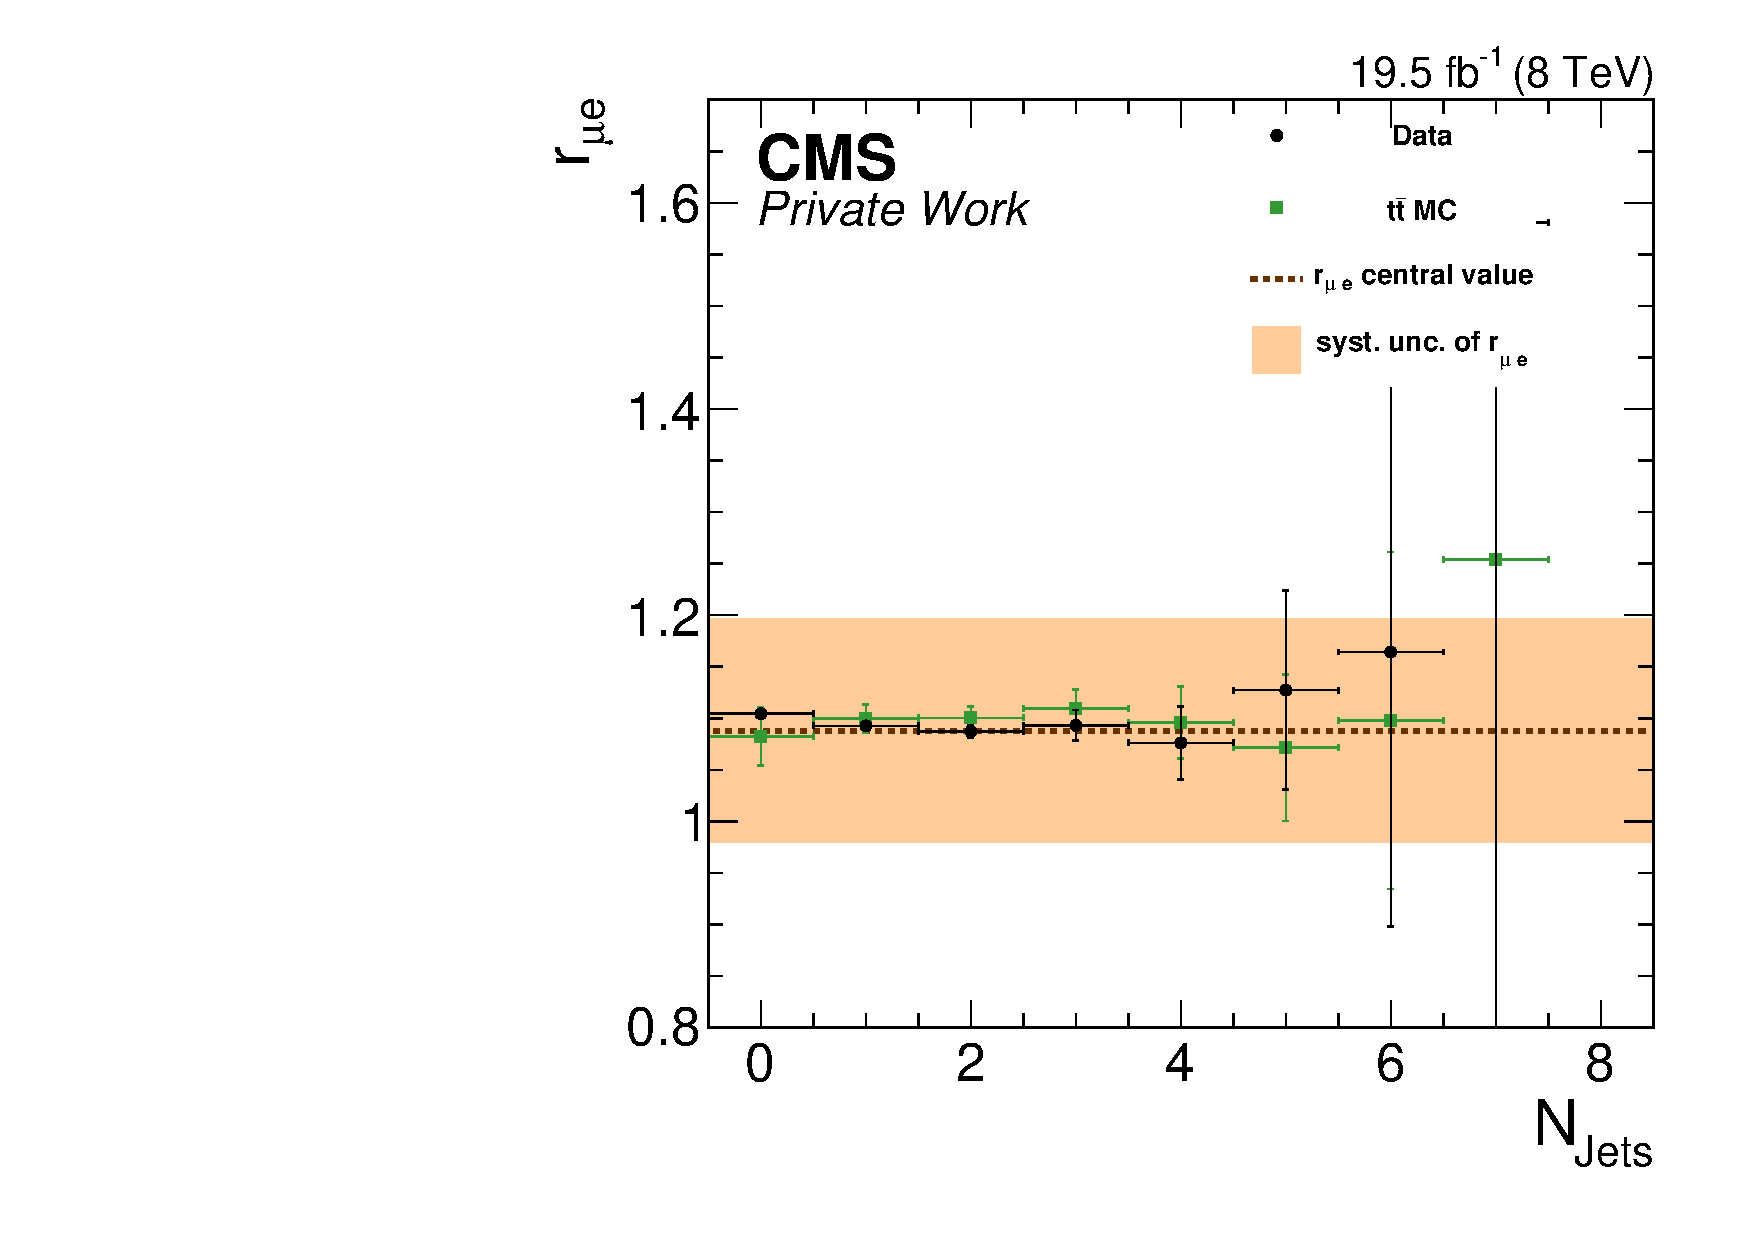
\includegraphics[width=\textwidth]{plots/BG/rmue/rMuE_ZPeakControlCentral_Full2012_NJets_None.pdf}
\end{minipage}
\begin{minipage}[t]{0.49\textwidth}
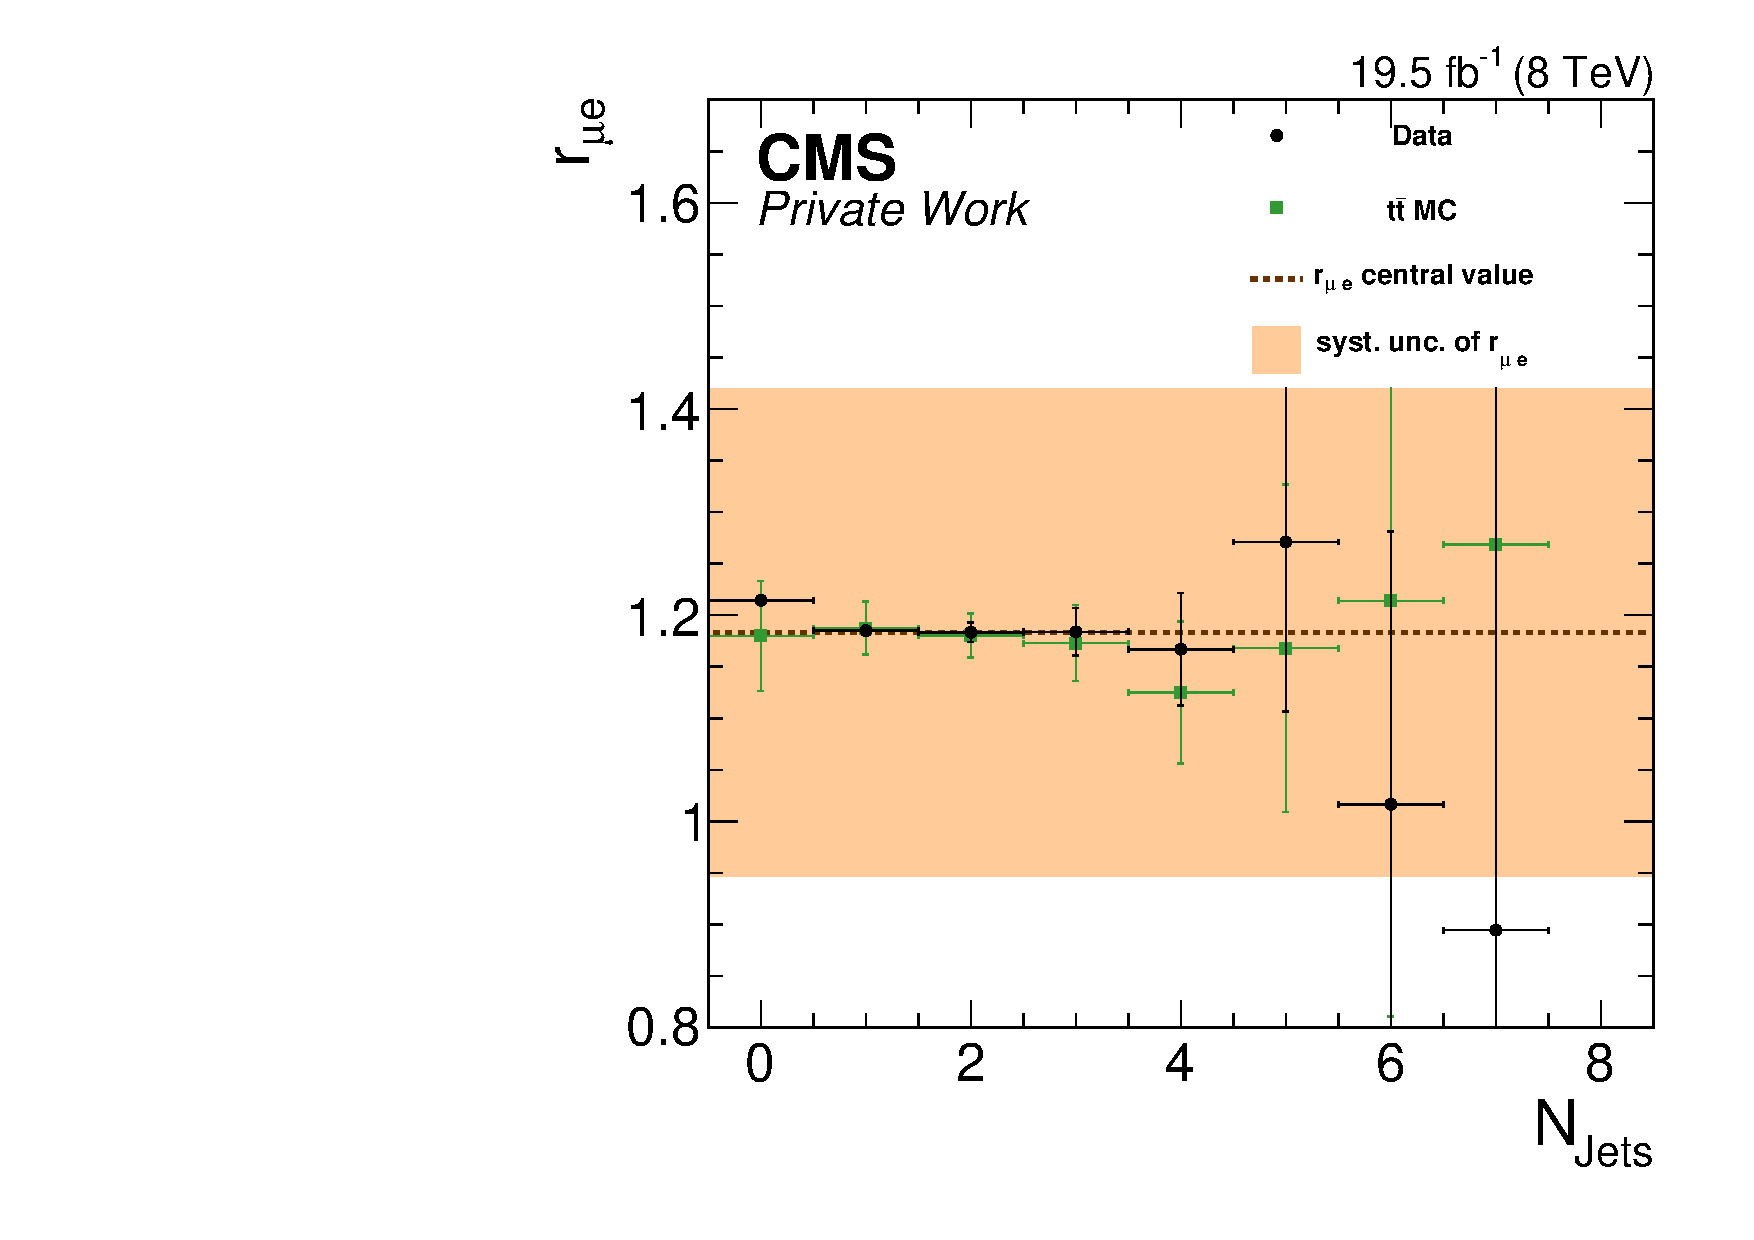
\includegraphics[width=\textwidth]{plots/BG/rmue/rMuE_ZPeakControlForward_Full2012_NJets_None.pdf}
\end{minipage}
\caption{Dependencies of \rmue on \mll (top), \MET (middle), and \njets (bottom) for the central (left) and forward (right) lepton selection. The results on data are shown in black while $t\bar{t}$ simulation is shown in green. The central value is shown as a brown dashed line while the assigned systematic uncertainty of 10\% for the central and 20\% for the forward lepton selection is shown as an orange band.}
\label{fig:rmueDependencies}
\end{figure} 
\subsubsection{Measurement of \RT}
\label{sec:triggerEffs}
The trigger efficiencies are measured utilizing an event sample collected with the \HT triggers discussed in Section~\ref{sec:trigger}. Lepton pairs corresponding to the flavour combination of the trigger in question are selected. To ensure that only correctly reconstructed events are considered in the calculation of the trigger efficiencies, the events are required to have $\HT > \unit{200}{\giga\electronvolt}$. This excludes events which are completely different in their properties on trigger and analysis level and at the same time is lower than the threshold applied in the trigger because the \HT definition on trigger level differs from the one used offline. To ensure that the factorisation method is performed on event samples completely orthogonal to the signal region and the flavour-symmetric control region, events with $\njets \geq 2$ and $\MET > \unit{100}{\giga\electronvolt}$ are rejected. This ensures that the direct measurement of \Rsfof and the factorisation method remain statistically independent. As the offline lepton selection has more strict requirements compared to the one applied at HLT level, the dilepton triggers should have accepted all these events. The trigger efficiency is therefore defined as the ratio of accepted events by the total number of events:
\begin{equation*}
\epsilon_{\ell\ell}^T = \frac{N_{\text{events}}(H_T\text{ trigger} \cap \ell\ell\text{ selection} \cap \ell\ell\text{ trigger})}{N_{\text{events}}(H_T\text{ trigger} \cap \ell\ell\text{ selection})}.
\end{equation*}
In case of \MM and OF events, two triggers are used in the event selection. Therefore, their combined efficiency is measured, requiring the logical OR of both. The resulting efficiencies are summarised in Table~\ref{tab:EffValues_Seperated}, separately for the central and forward lepton selections. As discussed in Section~\ref{sec:trigger}, the \HT triggers had to be prescaled during the data taking. The efficiencies on simulation are therefore measured with much higher statistical precision, as this prescales are not applied there. The trigger efficiencies for \EE and \MM are about 97\% in both the central and forward selection. The efficiency for OF events is lower, about 95\% in the central and 90\% in the forward selection. This shows how the flavour symmetry is broken at trigger level by the inclusion of the additional dimuon trigger, which recovers efficiency for the trailing muon leg of the trigger and is not present in the OF triggers.   

\begin{table}[hbp] \caption{Trigger efficiencies measured using \HT baseline trigger. The results are shown for the central and forward regions separately.} 
\centering 
\renewcommand{\arraystretch}{1.2} 
\begin{tabular}{l|c|c|c|c|c|c}     

 & nominator & denominator & $\epsilon_{\ell\ell}^{T} \pm \sigma_{\text{stat}}$ &  nominator & denominator & $\epsilon_{\ell\ell}^{T} \pm \sigma_{\text{stat}}$  \\ 
\hline

&\multicolumn{6}{c}{Data} \\
\hline
&  \multicolumn{3}{c|}{Central } & \multicolumn{3}{c}{ Forward }\\
\hline
ee & 3592 & 3692 & 0.973$\pm$0.003 & 954 & 980 & 0.973$\pm$0.006 \\
$\mu\mu$ & 1375 & 1420 & 0.968$\pm$0.005 & 547 & 566 & 0.966$\pm$0.009 \\
e$\mu$ & 493 & 521 & 0.946$\pm$0.012 & 102 & 114 & 0.895$\pm$0.037 \\
 
 
\hline

& \multicolumn{6}{c}{MC} \\
\hline
&  \multicolumn{3}{c|}{Central } & \multicolumn{3}{c}{ Forward } \\
\hline 
ee & 2912.8 & 2994.6 & 0.973$\pm$0.001 & 943.0 & 969.9 & 0.972$\pm$0.001 \\
$\mu\mu$ & 3241.6 & 3287.9 & 0.986$\pm$0.001 & 1141.6 & 1183.4 & 0.965$\pm$0.001 \\
e$\mu$ & 6279.1 & 6523.1 & 0.963$\pm$0.001 & 2138.8 & 2249.0 & 0.951$\pm$0.001 \\
    
    \hline 
\end{tabular}  
\label{tab:EffValues_Seperated}
\end{table}	

To assess the systematic uncertainties of the trigger efficiency measurement, potential biases due to the choice of the orthogonal trigger  are studied on simulation, using dileptonic $t\bar{t}$ events. On simulation the efficiency can be measured without the requirement of the \HT triggers, as no trigger is needed to select the events. The ratio of the efficiencies measured with the \HT triggers to those true efficiencies as a function of \mll is shown on the left side of Figure~\ref{fig:triggerEffBias}, separately for SF and OF events. In both cases all deviations from unity are in the order of 0.1\% and well compatible with unity inside the statistical uncertainties. No bias of the efficiency measurement due to the \HT triggers is observed and therefore no systematic uncertainty due to this choice is assigned to the measurement.
\begin{figure}
\begin{center}
\begin{minipage}[t]{0.49\textwidth}
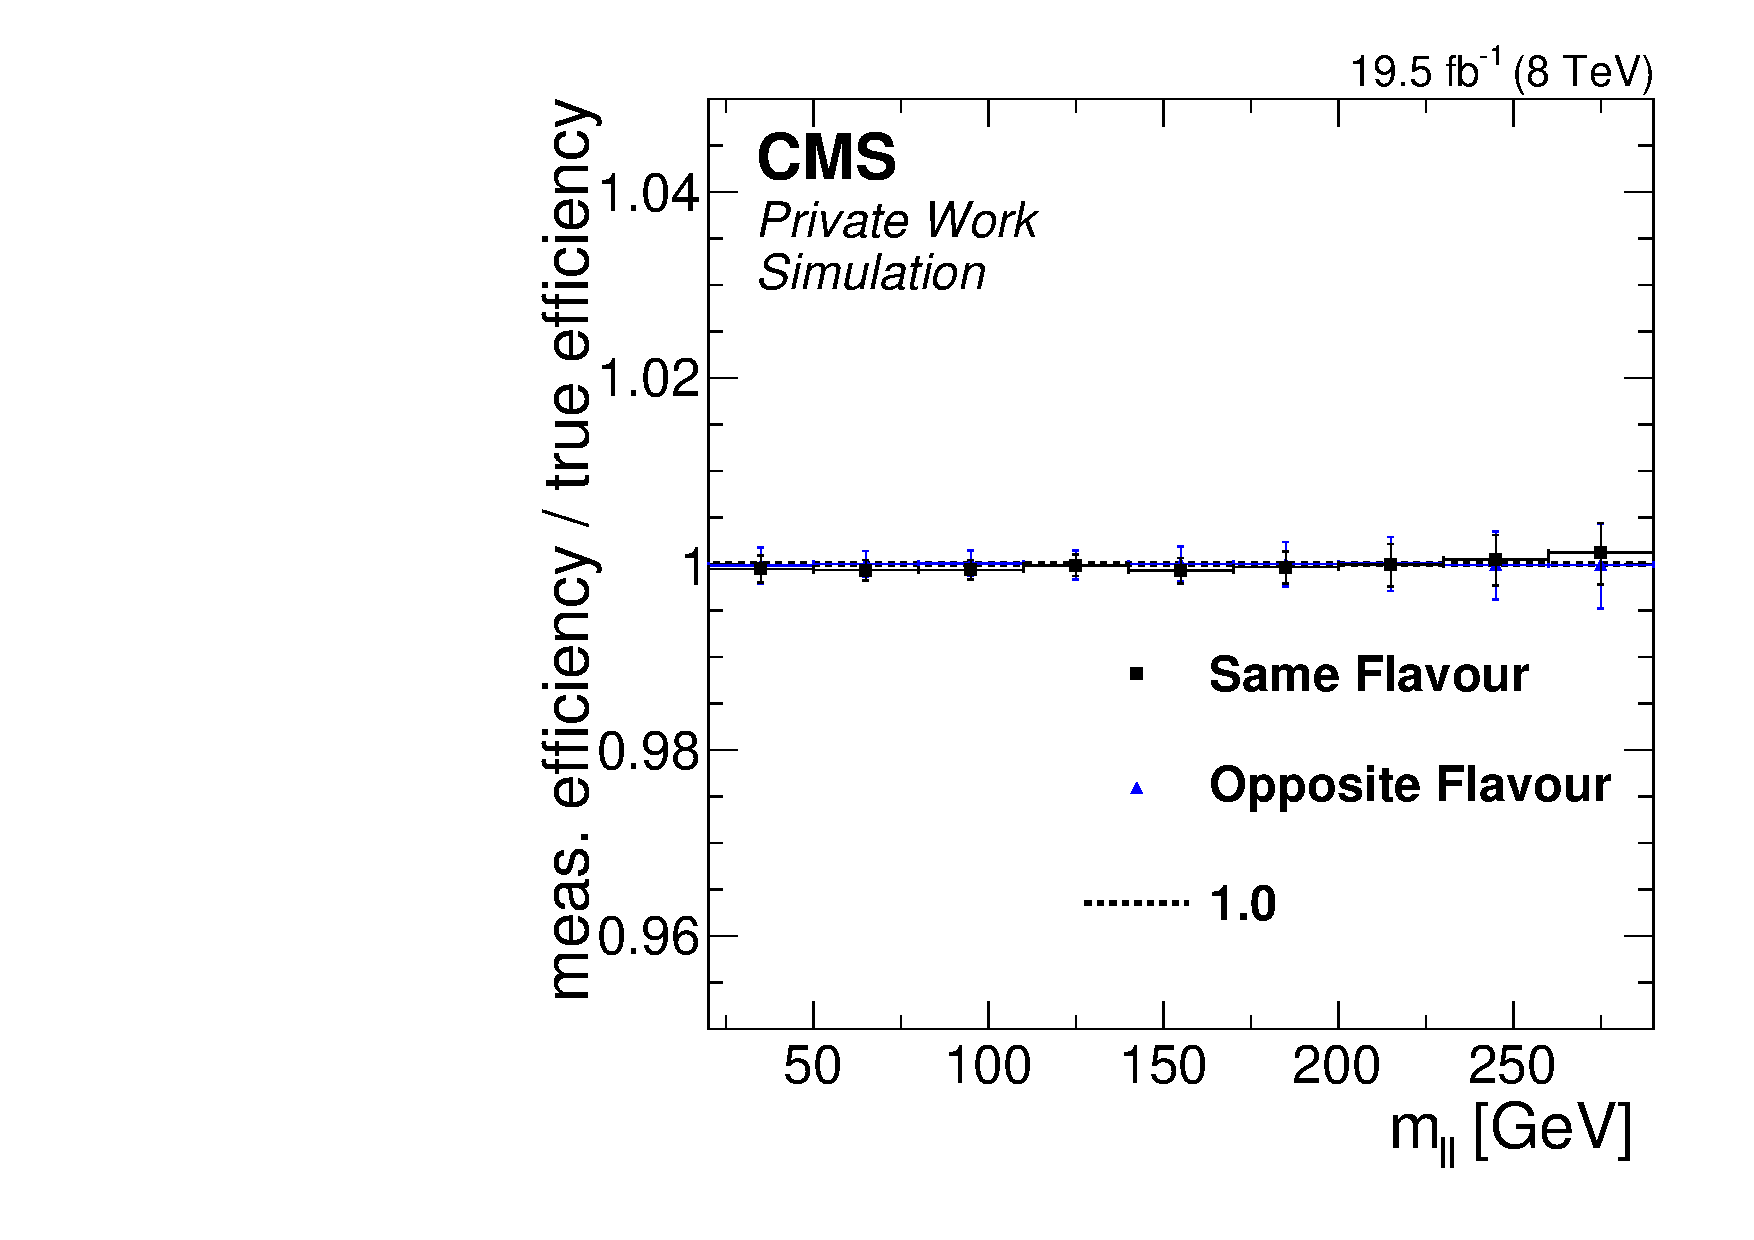
\includegraphics[scale=0.375]{plots/BG/trigger/Triggereff_AlphaTSyst_PFHT_HighHTExclusive_Full2012_Mll_None.pdf}
\end{minipage}
\begin{minipage}[t]{0.49\textwidth}
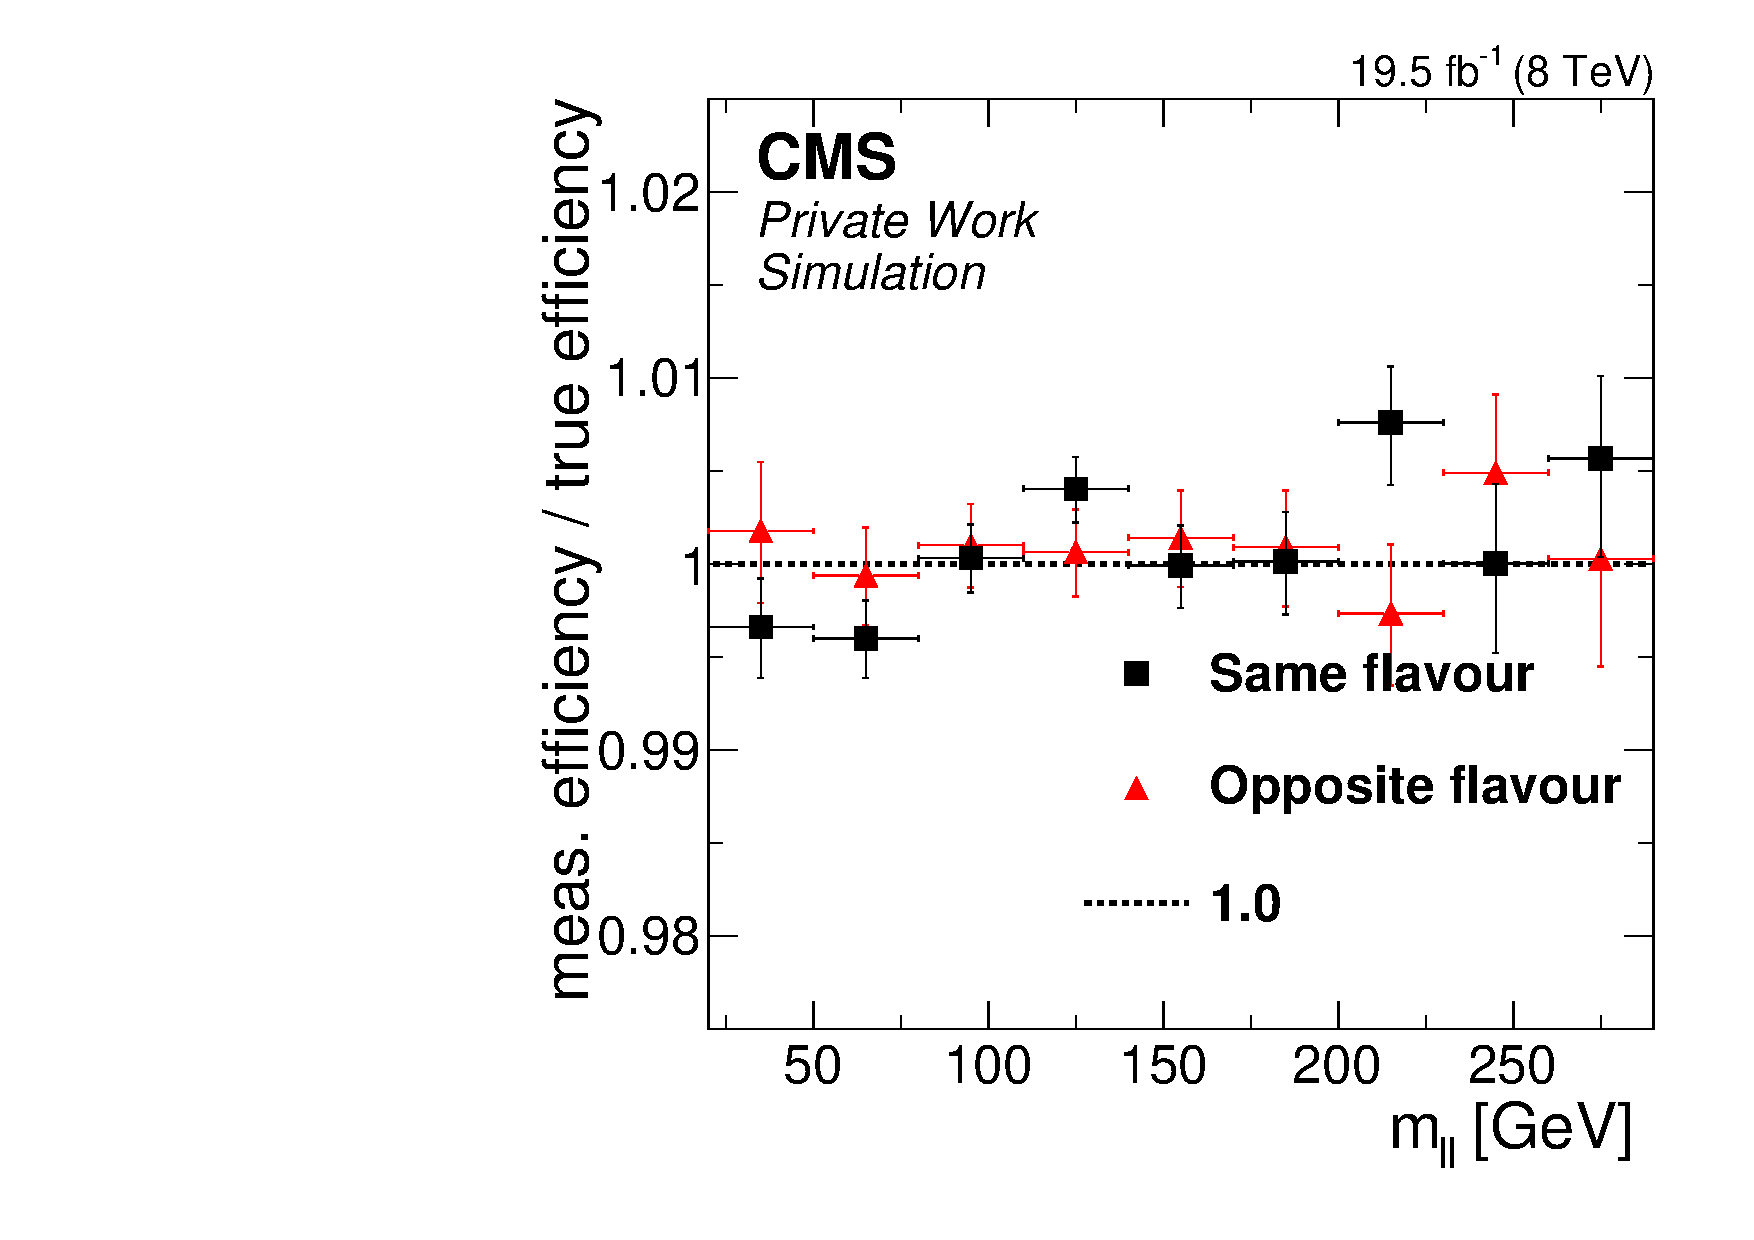
\includegraphics[scale=0.375]{plots/BG/trigger/Triggereff_AlphaTSyst_AlphaT_HighHTExclusive_Full2012_Mll_None.pdf}
\end{minipage}
\caption{The ratio of trigger efficiencies calculated using the \HT ($\alpha_{\mathrm{T}}$) triggers to the true efficiencies is shown on the left (right) side, separately for SF and OF events.}
\label{fig:triggerEffBias}
\end{center}
\end{figure}

The turn-on of the triggers at low lepton \pt is of particular interest because asymmetries between the lepton flavours are more likely to occur in this difficult environment. The dependence of the trigger efficiency on the \pt of the trailing lepton can be studied using datasets triggered by single lepton triggers. Triggers with \pt thresholds of $\unit{24 (27)}{\giga\electronvolt}$ for muons (electrons) are available. These thresholds are relatively low for single lepton triggers, resulting in very strict selection criteria applied on HLT level. Dilepton events are selected, in which the leading lepton can be matched  geometrically to the trigger object that fired the single lepton trigger. The trailing lepton is matched to trigger objects that have fired the trailing leg of the dilepton trigger. The efficiency is defined as the ratio of the number of events in which the dilepton trigger has fired, over the total number of dilepton events. The resulting efficiency curves are shown in Figure~\ref{fig:triggerEffTrailing} for four different trailing lepton trigger legs and combining the central and forward selection. The asymptotic efficiency for trailing electrons is virtually the same for the dielectron and OF triggers (black and light blue markers). The same is not true for trailing muons in the dimuon and OF triggers (red and dark blue markers), caused by the increased efficiency for trailing muons in the $\mu\mu$ channel, which is significantly higher than those in the trigger paths not using the tracker information, as expected. Trailing muons have a much sharper turn-on than trailing electrons and are fully efficient already at a \pt of $\unit{10}{\giga\electronvolt}$. For electrons the plateau is reached only at about $\unit{\approx 30}{\giga\electronvolt}$. The turn-on is steeper for trailing electrons in the dielectron trigger compared to those in the OF trigger, resulting in an increased deviation from flavour symmetry below $\unit{20}{\giga\electronvolt}$. As the precision and stability of the background prediction was given priority over lepton acceptance in the design of the analysis, events with trailing leptons in this \pt range are rejected.  
\begin{figure}
\begin{center}
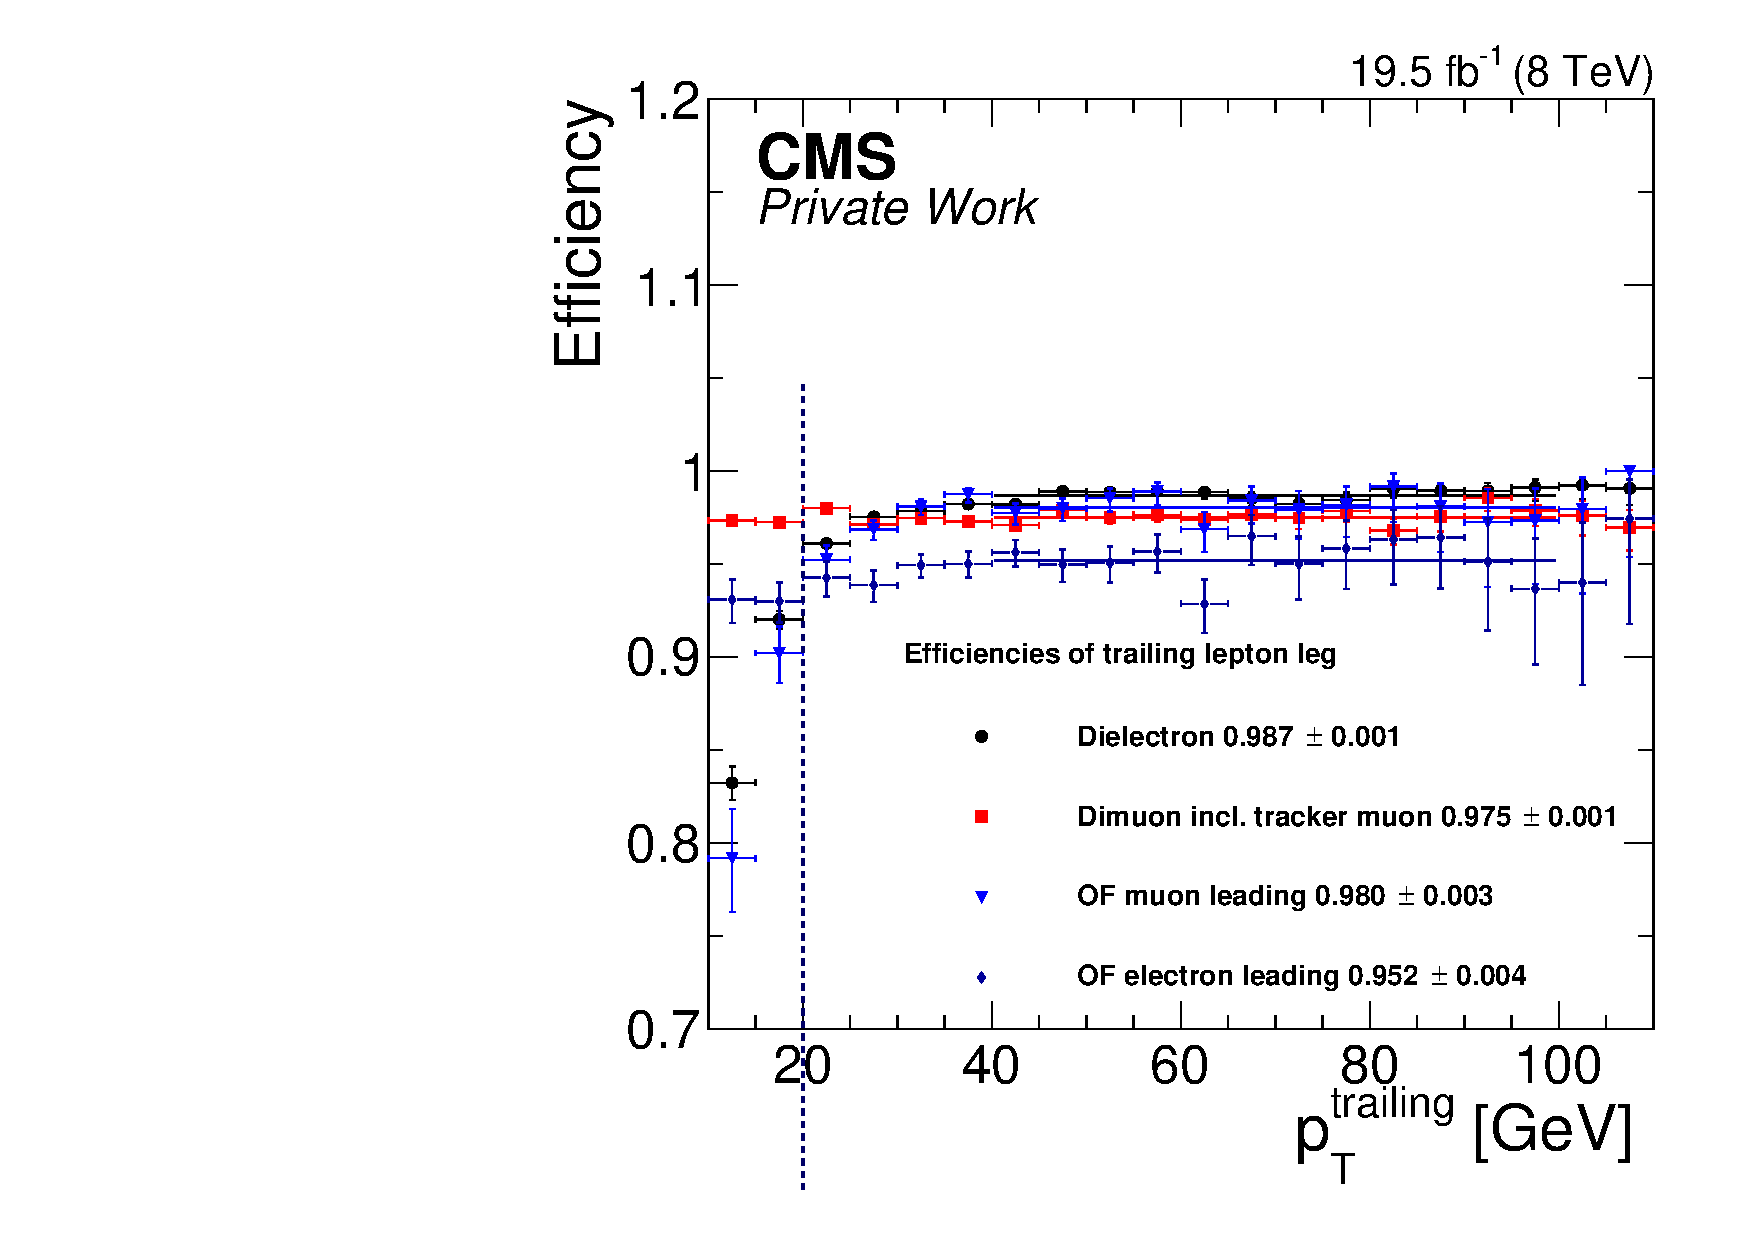
\includegraphics[scale=0.45]{plots/BG/trigger/Triggereff_SingleLepton_HighHTExclusive_Full2012_TrailingPt_leadingPt30Single.pdf}
\caption{Efficiency of the trailing lepton legs of the dilepton trigger measured on a sample of data events selected with single lepton triggers as a function of the \pt of the trailing lepton. The asymptotic efficiency with its statistical uncertainties are determined by fitting a constant in the range $\unit{\pt > 40}{\giga\electronvolt}$.}
\label{fig:triggerEffTrailing}
\end{center}
\end{figure} 

To assess the systematic uncertainties of the trigger efficiency measurement, the dependency of \RT, as used in the calculation of \Rsfof, on different observables is tested. Here a dataset triggered by $\alpha_\mathrm{T}$ triggers is used, as the \HT triggers do not provide enough events for these studies. The use of these triggers is motivated by the fact that they also rely on hadronic event properties and are therefore exhibit no significant correlation with the dilepton triggers, as is the case with the \HT triggers. This is illustrated on the right side of Figure~\ref{fig:triggerEffBias}, where the efficiencies measured using the $\alpha_{\mathrm{T}}$ triggers are compared to the true efficiency as a function of \mll. As $\alpha_{\mathrm{T}}$ is designed to suppress SM backgrounds, the available statistics for this test is low compared to the case of the \HT triggers. However, no significant deviation from unity is observed, which validates the use of the $\alpha_{\mathrm{T}}$ triggers for this studies.

A 5\% systematic uncertainty is assigned to each trigger efficiency, resulting in an uncertainty of 6.4\% on \RT, covering all observed deviations from the measured value of \RT within the statistical uncertainties, as shown in Figure~\ref{fig:RTDependencies}. Studies of further variables can be found in Appendix~\ref{app:RT}. The mean \RT values displayed in the figures are obtained using the $\alpha_{\mathrm{T}}$ trigger as baseline and therefore differ from the nominal result obtained using the \HT triggers. 
\begin{figure}[htbp]
\centering
\begin{minipage}[t]{0.49\textwidth}
  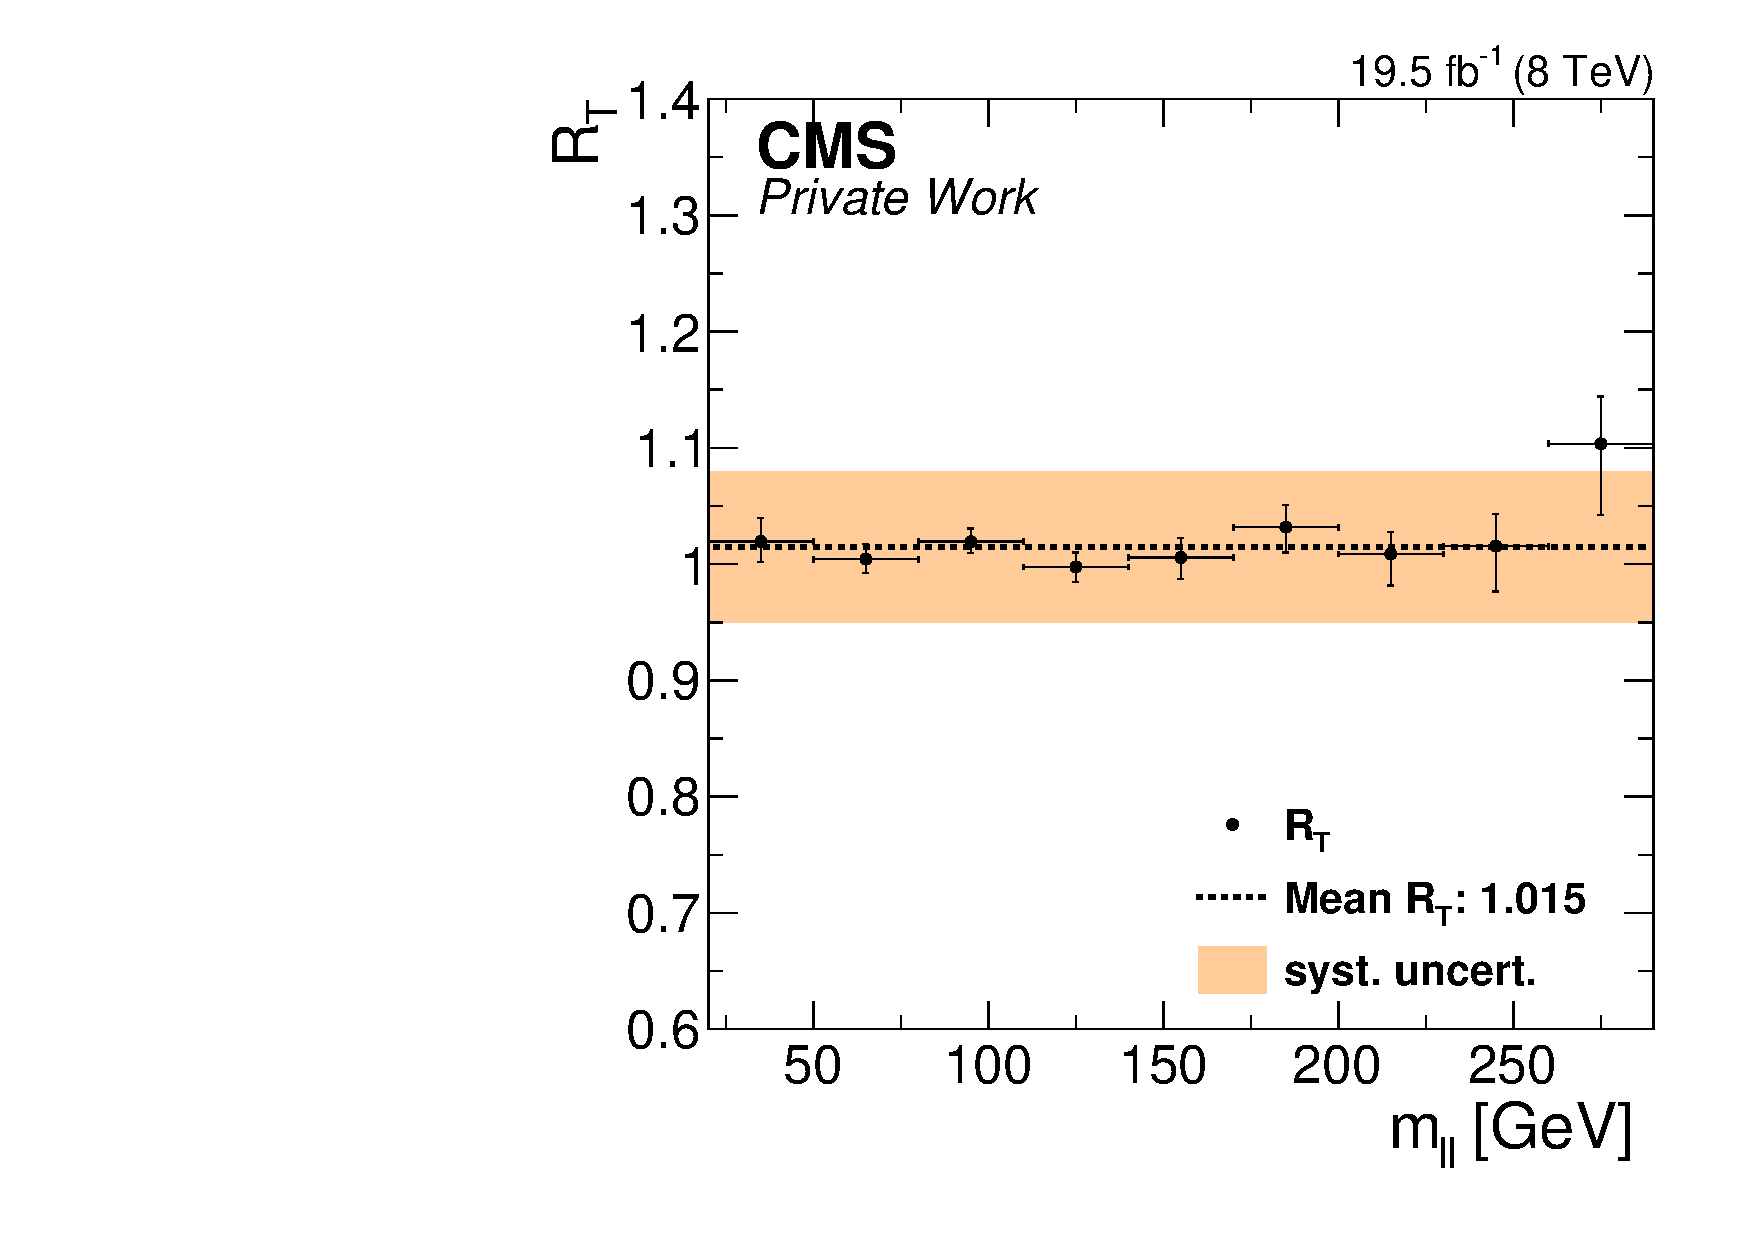
\includegraphics[width=\textwidth]{plots/BG/trigger/Triggereff_SFvsOF_Syst_AlphaT_HighHTExclusiveCentral_Full2012_Mll_None.pdf}
\end{minipage}
\begin{minipage}[t]{0.49\textwidth}
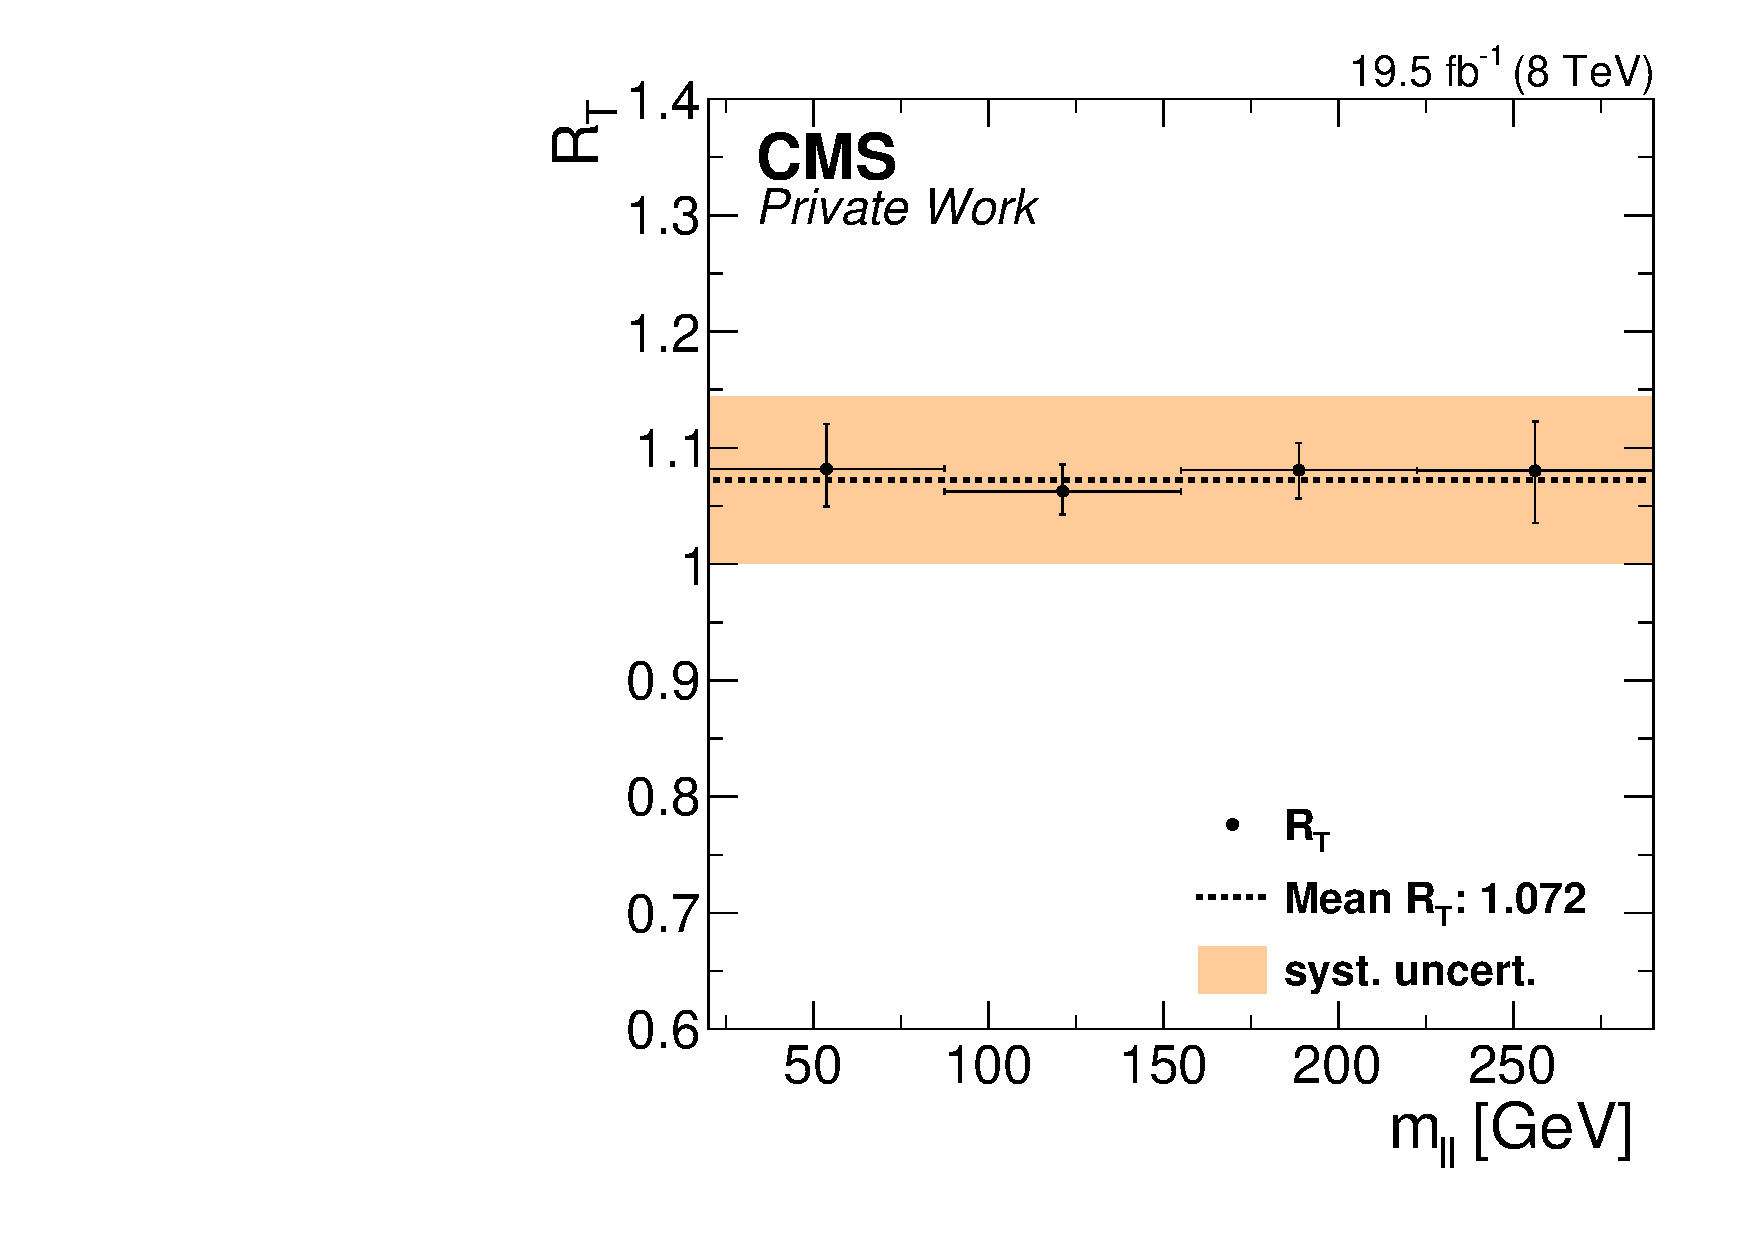
\includegraphics[width=\textwidth]{plots/BG/trigger/Triggereff_SFvsOF_Syst_AlphaT_HighHTExclusiveForward_Full2012_Mll_None.pdf}
\end{minipage}
\begin{minipage}[t]{0.49\textwidth}
  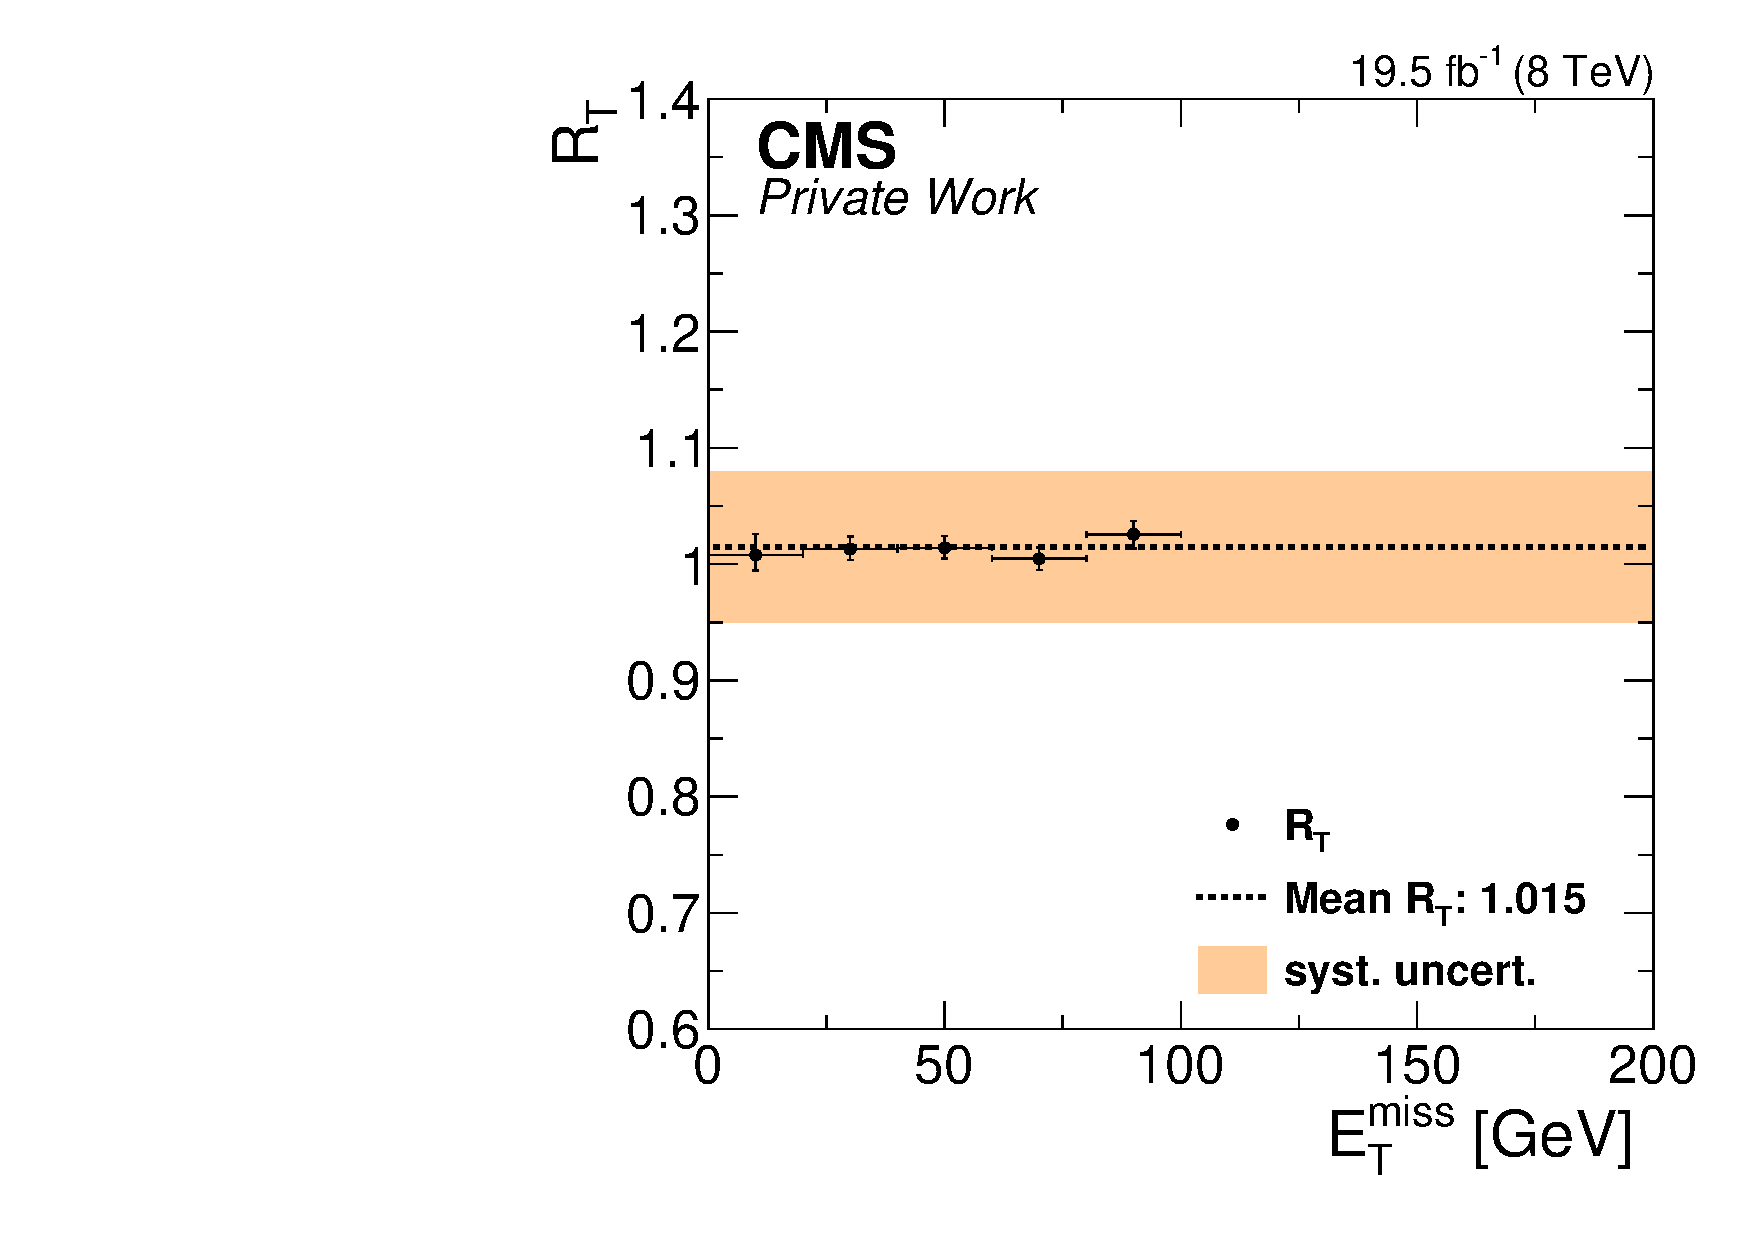
\includegraphics[width=\textwidth]{plots/BG/trigger/Triggereff_SFvsOF_Syst_AlphaT_HighHTExclusiveCentral_Full2012_MET_None.pdf}
\end{minipage}
\begin{minipage}[t]{0.49\textwidth}
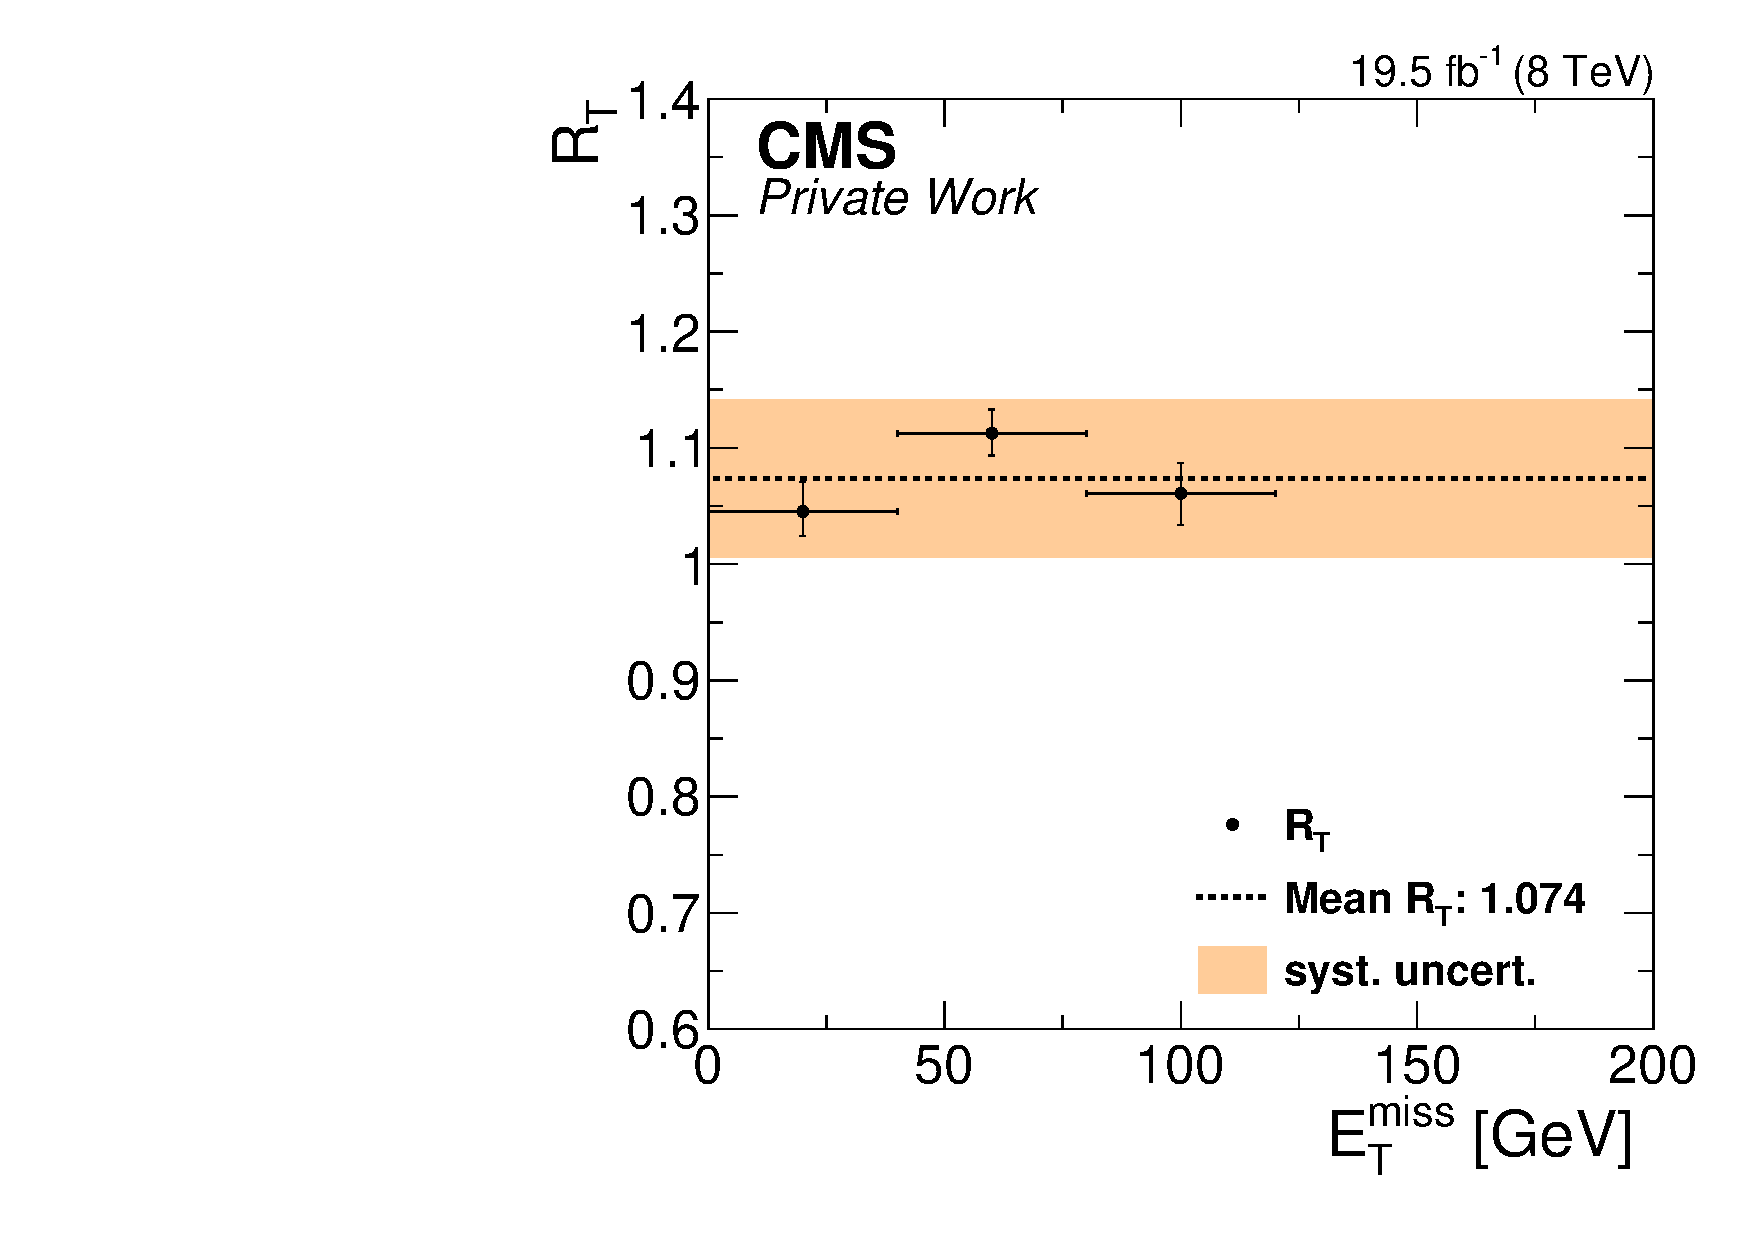
\includegraphics[width=\textwidth]{plots/BG/trigger/Triggereff_SFvsOF_Syst_AlphaT_HighHTExclusiveForward_Full2012_MET_None.pdf}
\end{minipage}
\begin{minipage}[t]{0.49\textwidth}
  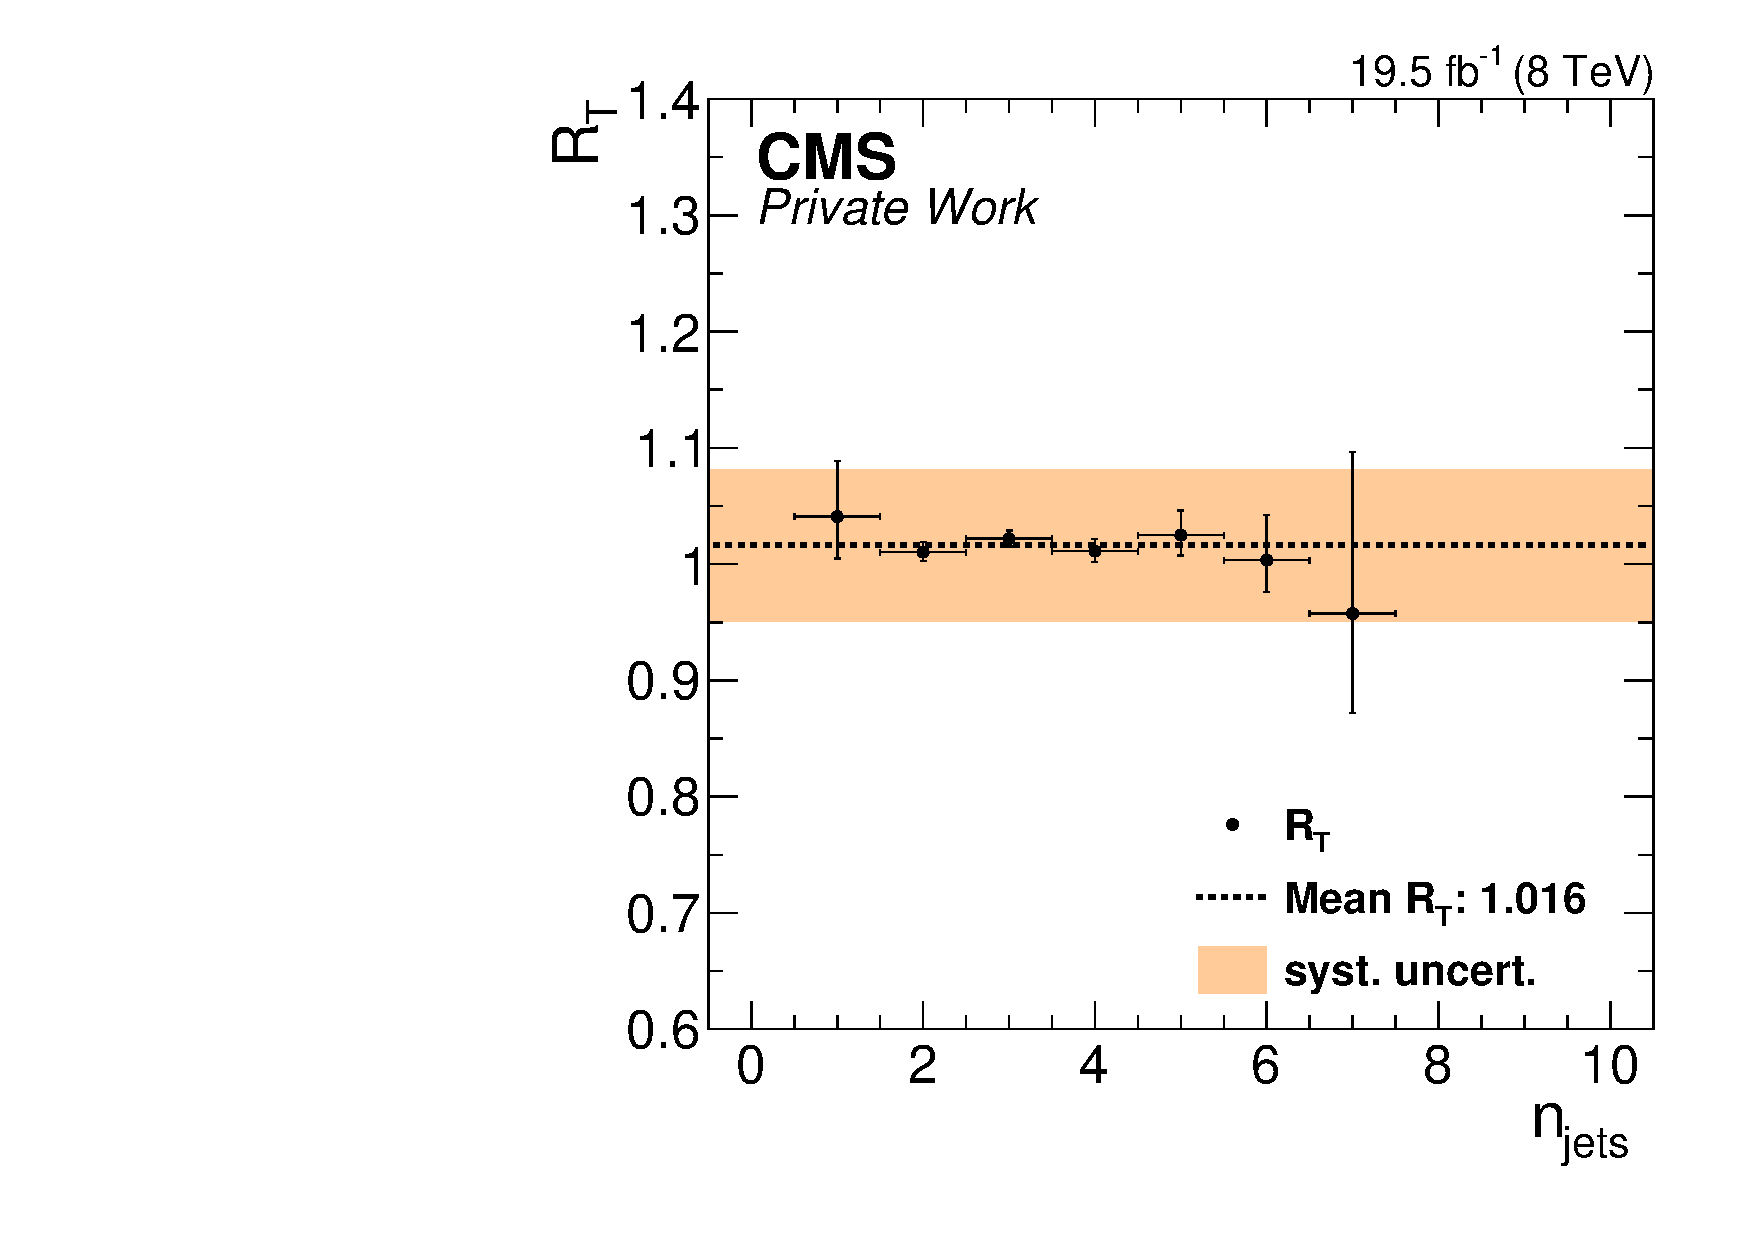
\includegraphics[width=\textwidth]{plots/BG/trigger/Triggereff_SFvsOF_Syst_AlphaT_HighHTExclusiveCentral_Full2012_NJets_None.pdf}
\end{minipage}
\begin{minipage}[t]{0.49\textwidth}
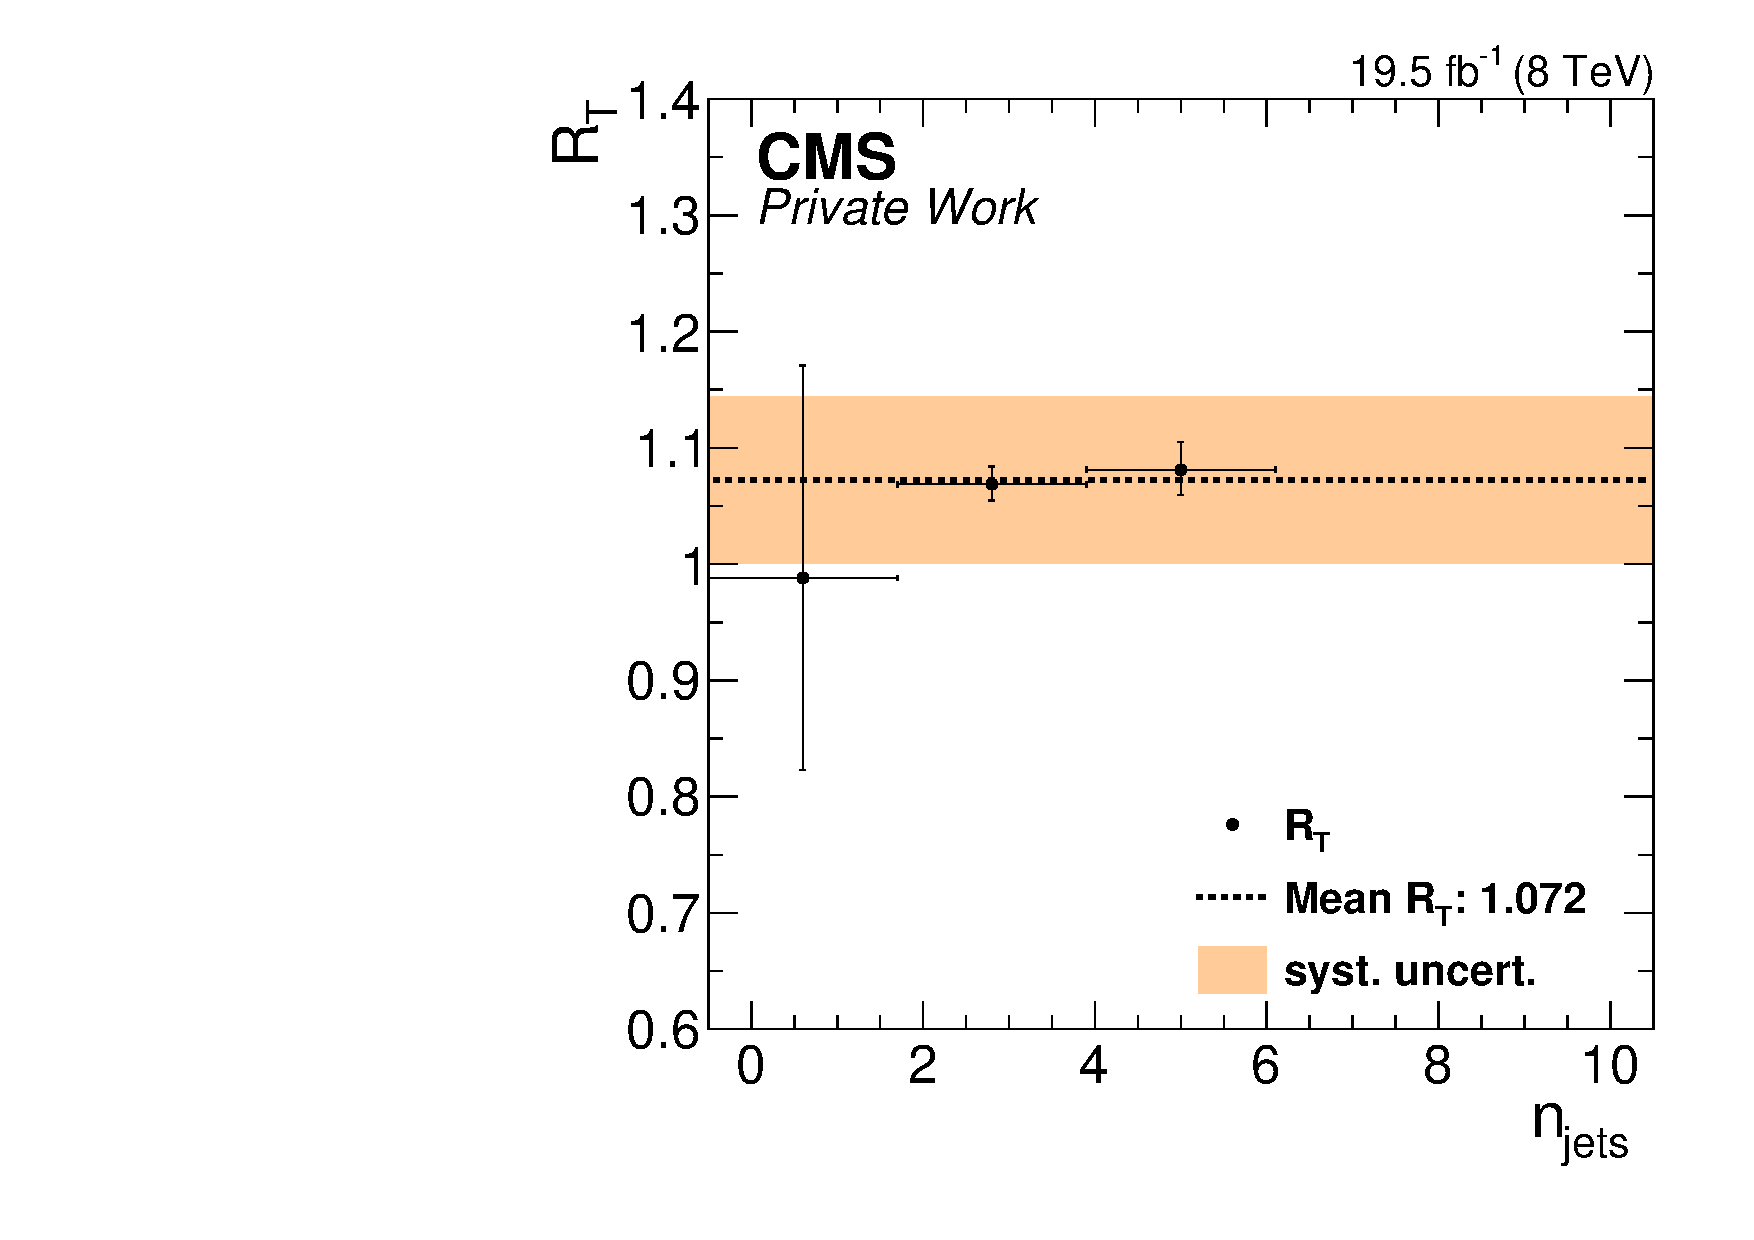
\includegraphics[width=\textwidth]{plots/BG/trigger/Triggereff_SFvsOF_Syst_AlphaT_HighHTExclusiveForward_Full2012_NJets_None.pdf}
\end{minipage}
\caption{Dependencies of \RT on \mll (top), \MET (middle), and \njets (bottom) for the central (left) and forward (right) lepton selection. The $\alpha_{\mathrm{T}}$ triggers are used as baseline trigger to select the events. The results on data are shown in black. The central value is shown as a black dashed line while the systematic uncertainty is shown as an orange band.}
\label{fig:RTDependencies}
\end{figure} 
\subsubsection{Results of the factorisation method}
The results of the factorisation methods are summarised in Table~\ref{tab:factorisation}. The factor $R_T$ is calculated from the trigger efficiencies in Table~\ref{tab:EffValues_Seperated} via Equation~\ref{eq:RT}. The resulting correction factors \Rsfof, \Reeof, and \Rmmof are calculated as described in Equations~\ref{eq:nee}-\ref{eq:nsf}.  

\begin{table}[hbtp]
 \renewcommand{\arraystretch}{1.3}
 \setlength{\belowcaptionskip}{6pt}
 \centering
 \caption{Result of the determination of \Rsfof, \Reeof, and \Rmmof using the factorisation method.}
  \label{tab:factorisation}
  \begin{tabular}{l| c c| c c }

    & \multicolumn{2}{c}{Central} & \multicolumn{2}{c}{Forward} \\ 
    								
    \hline
    & Data & MC & Data & MC \\ 
 
    \hline
        \rmue       &  1.088$\pm$0.109  &  1.103$\pm$0.110      &  1.183$\pm$0.237 &   1.207$\pm$0.241    \\
        $R_{T}$       &  1.026$\pm$0.066  &  1.017$\pm$0.065      &  1.084$\pm$0.079 &   1.018$\pm$0.069    \\

\hline
\hline
        \Rsfof       &  1.029$\pm$0.067  &  1.031$\pm$0.067      &  1.099$\pm$0.088 &   1.103$\pm$0.091    \\
        \Reeof       &  0.471$\pm$0.116  &  0.465$\pm$0.117      &  0.458$\pm$0.259 &   0.449$\pm$0.264    \\
        \Rmmof       &  0.558$\pm$0.117  &  0.565$\pm$0.119      &  0.641$\pm$0.261 &   0.654$\pm$0.266    \\

  \end{tabular}
\end{table}



As for the direct measurements in the control region, the observed deviations of \Rsfof from one are small and inside the uncertainties of the method in the central region. In the forward region, a deviation from unity of 10\% is observed both on data and in simulation, as expected from the larger differences in the efficiencies of electrons and muons in this region. Because the uncertainty on \rmue cancels out to a large degree in the calculation \Rsfof, the total uncertainty is dominated by the uncertainty on \RT, while for \Reeof and \Rmmof the uncertainty of \rmue is the dominant one. This results in much larger uncertainties on the latter two factors. The dependency of \Rsfof on \rmue and \RT as given by Equation~\ref{eq:nsf} is illustrated in Figure~\ref{fig:rmuePropaganda}. The measured values of \rmue and \Rsfof are shown as straight lines, surrounded by bands indicating their uncertainties. The red line shows the value of \Rsfof corresponding to a given \rmue, under the assumption that the trigger efficiencies stay constant. The dashed black lines show the impact, that the uncertainties on the trigger efficiencies have on the resulting \Rsfof. It can be seen that variations of \rmue inside the systematic uncertainties have only little effect on \Rsfof, while changes in the trigger efficiencies have a much larger impact. 


\begin{figure}[htbp]
\centering
\begin{minipage}[t]{0.49\textwidth}
  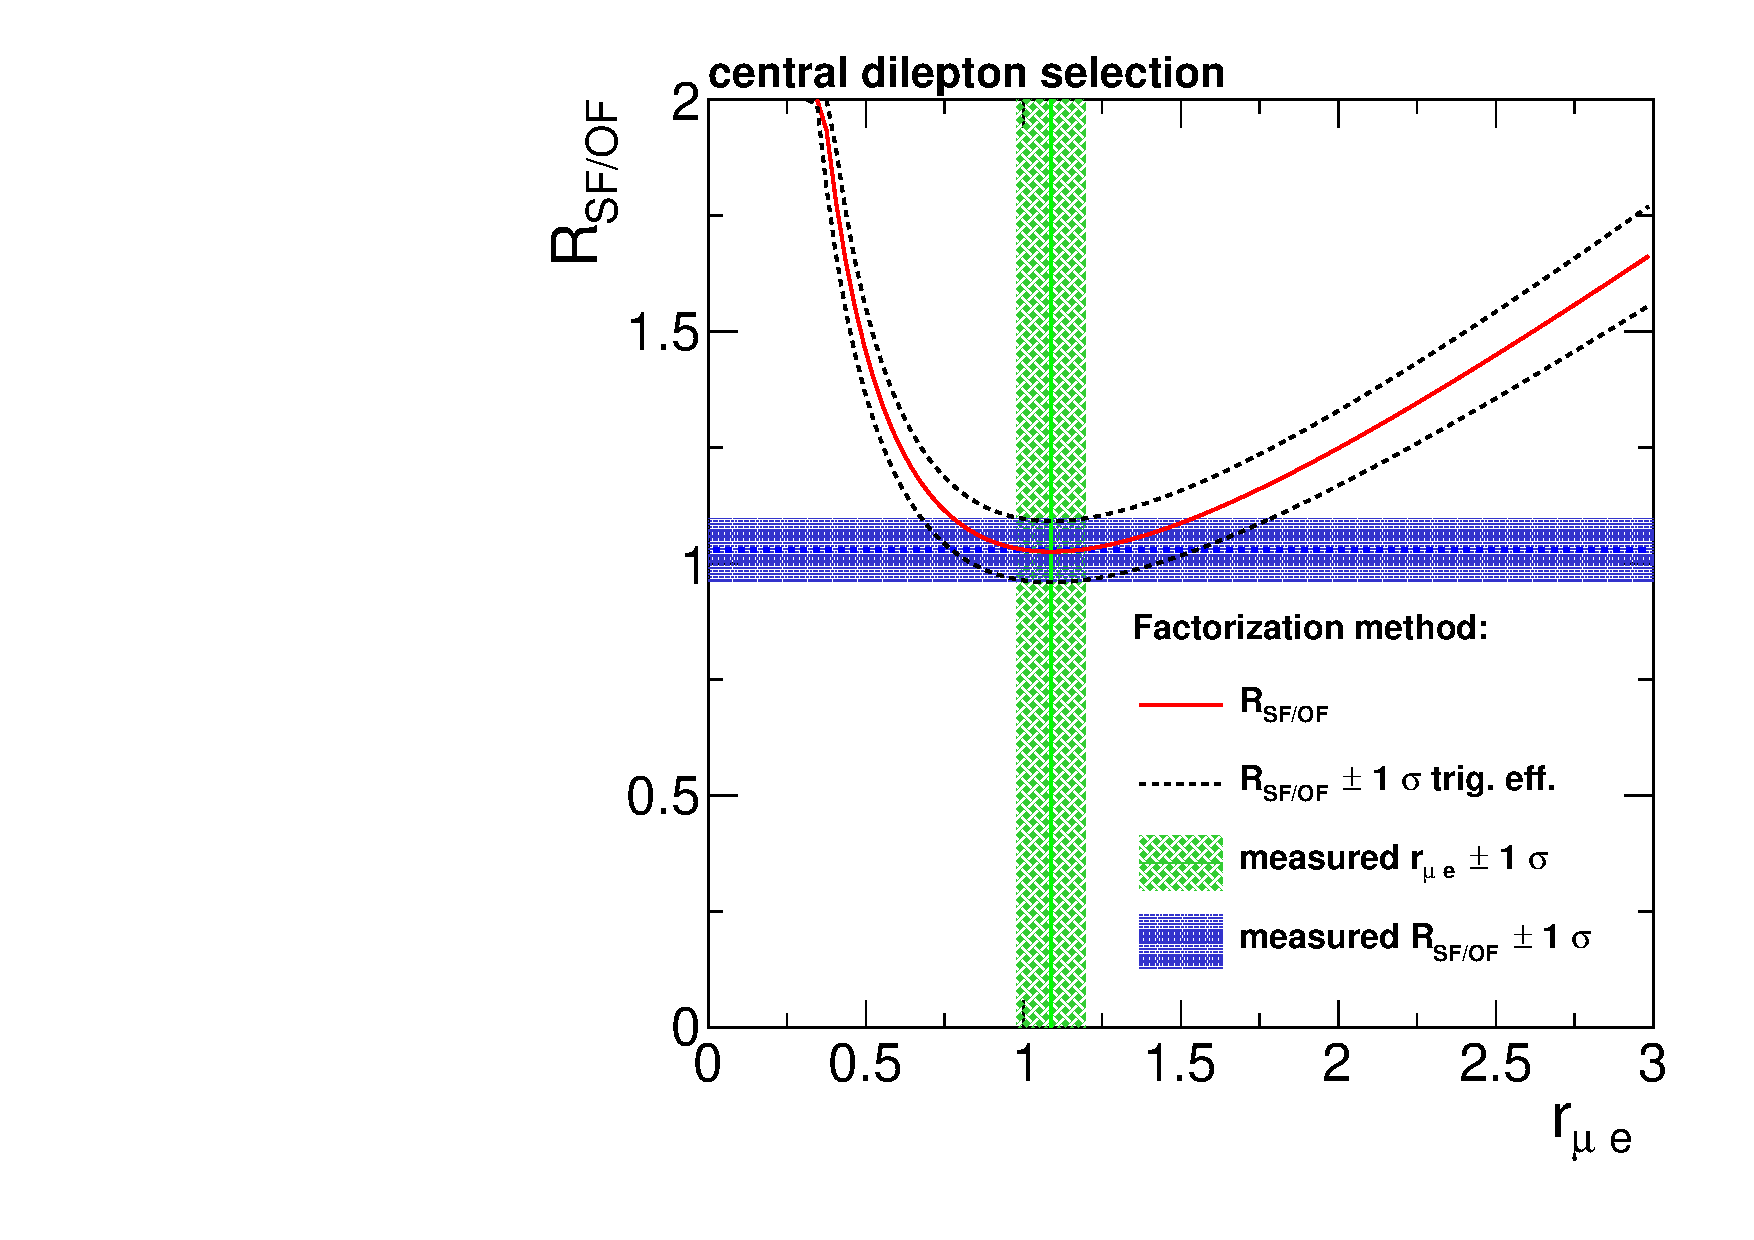
\includegraphics[width=\textwidth]{plots/BG/rmue/rMuEPropaganda_central.pdf}
\end{minipage}
\begin{minipage}[t]{0.49\textwidth}
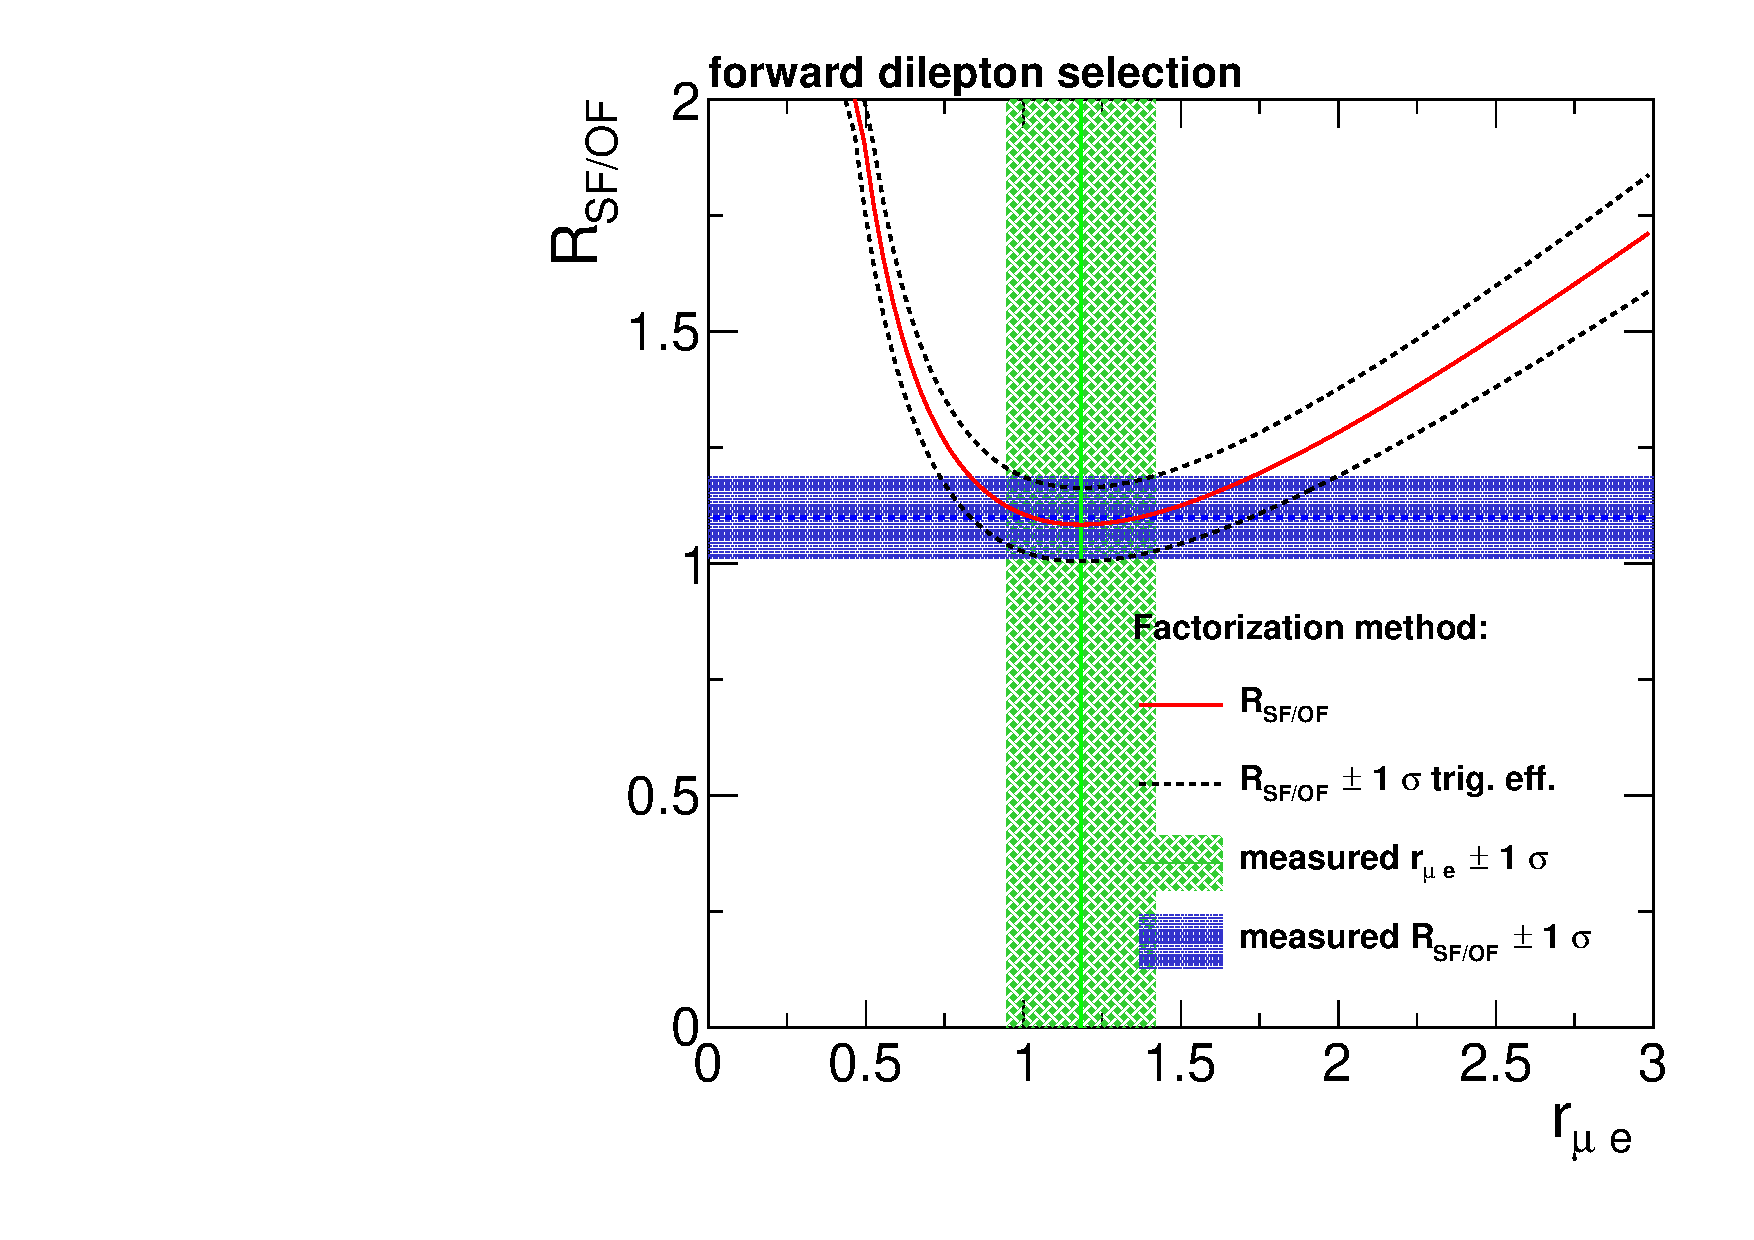
\includegraphics[width=\textwidth]{plots/BG/rmue/rMuEPropaganda_forward.pdf}
\end{minipage}

\caption{Dependency of \Rsfof on \rmue in the factorisation method. The measured central values of \Rsfof and \rmue and their uncertainty are shown as the blue and green lines and bands. The red line illustrates the value of \Rsfof for a given \rmue if \RT is kept constant. The impact of a variation of \RT within its uncertainties on \Rsfof is shown by the dashed black lines.}
\label{fig:rmuePropaganda}
\end{figure} 

\subsection{Combined correction factors and resulting background estimates}
\label{sec:combinedRSFOF}
An overview of the resulting corrections factors of the measurement in the control region and the factorisation method are shown in Table~\ref{tab:combinedRSFOF}. In all cases the results of the two methods agree very well within their uncertainties. 

Given the fact that they are performed on exclusive datasets and under the assumption that their uncertainties follow a Gaussian distribution, which is justified by the fact that they are either statistical in nature (and the samples sizes are sufficiently large), or assigned to cover statistical fluctuations in the dependency studies of \rmue and \RT, they can be combined using a weighted average. 

\begin{table}[hbtp]
 \renewcommand{\arraystretch}{1.3}
 \setlength{\belowcaptionskip}{6pt}
 \scriptsize
 \centering
 \caption{
     }
  \label{tab:combinedRSFOF}
  \begin{tabular}{l| c c| c c }
    & \multicolumn{4}{c}{\Rsfof}  \\ 

    & \multicolumn{2}{c}{Central} & \multicolumn{2}{c}{Forward} \\ 
    								
    \hline
    & Data & MC & Data & MC \
    \hline
        from factorization method       &  1.029\pm0.067  &  1.023\pm0.065      &  1.099\pm0.088 &   1.037\pm0.077    \\
        from direct measurement       &  1.012\pm0.039  &  1.010\pm0.008      &  1.000\pm0.105 &   1.010\pm0.014    \\
        weighted avarage       &  1.016\pm0.034  &  1.010\pm0.008      &  1.034\pm0.052 &   1.011\pm0.014    \\

\hline
    & \multicolumn{4}{c}{\Reeof}  \\ 

    & \multicolumn{2}{c}{Central} & \multicolumn{2}{c}{Forward} \\ 
    								
    \hline
    & Data & MC & Data & MC \
    \hline
        from factorization method       &  0.471\pm0.116  &  0.460\pm0.116      &  0.458\pm0.259 &   0.421\pm0.248    \\
        from direct measurement       &  0.459\pm0.026  &  0.457\pm0.005      &  0.439\pm0.093 &   0.427\pm0.008    \\
        weighted avarage       &  0.459\pm0.023  &  0.457\pm0.005      &  0.439\pm0.038 &   0.427\pm0.008    \\

\hline
    & \multicolumn{4}{c}{\Rmmof}  \\ 

    & \multicolumn{2}{c}{Central} & \multicolumn{2}{c}{Forward} \\ 
    								
    \hline
    & Data & MC & Data & MC \
    \hline
        from factorization method       &  0.558\pm0.117  &  0.563\pm0.118      &  0.641\pm0.261 &   0.617\pm0.250    \\
        from direct measurement       &  0.553\pm0.028  &  0.553\pm0.005      &  0.561\pm0.095 &   0.582\pm0.009    \\
        weighted avarage       &  0.553\pm0.026  &  0.553\pm0.005      &  0.563\pm0.043 &   0.582\pm0.009    \\

\hline
  \end{tabular}
\end{table}


 
A precision of about 4\% and 6\% on the translation from opposite flavour to same flavour is reached in the central and forward dilepton selection, respectively. Separating the lepton flavours, the uncertainty in \Reeof and \Rmmof is about 6\% for central and 9-10\% for forward leptons. This increase is caused by the missing cancellation of the uncertainty on \rmue and the increased statistical uncertainty in the direct measurement in the control region. However, only \Rsfof is used in the background estimates for both counting experiment and the shape analysis and the separate \EE and \MM channels are only studied as cross-checks. Therefore, the increased uncertainty in the separate channels has no impact on the sensitivity of the result.

Given that the weighted average is calculated separately for each flavour combination, \Reeof and \Rmmof do not add up exactly to \Rsfof, which in turn means that the sum of the background estimates for flavour-symmetric backgrounds in the \EE and \MM channels does not equal that in the SF channel. The OF yields in the \mll bins of the counting experiment together with the resulting background estimates in the different dilepton channels are shown in Table~\ref{tab:FlavSymBackgrounds}. 

\begin{table}[hbtp]
 \renewcommand{\arraystretch}{1.3}
 \setlength{\belowcaptionskip}{6pt}
 \scriptsize
 \centering
 \caption{Resulting estimates for flavour-symmetric backgrounds. Given is the observed event yield in OF events and the resulting estimate after applying the correction, separately for the SF, \EE, and \MM channels. Statistical and systematic uncertainties are given separately.
     }
  \label{tab:FlavSymBackgrounds}
  \begin{tabular}{l| cc | cc | cc}
    							& \multicolumn{2}{c}{Low-mass} & \multicolumn{2}{c}{On-\Z} & \multicolumn{2}{c}{High-mass} \\ 

    \hline
                                &  Central        & Forward  &  Central  & Forward   &  Central        & Forward \\ 

    \hline
        Observed OF events       &  737                   & 138              &  364            &  131       &   779           &   393    \\

    \hline
        Estimate in SF channel    & $746\pm27\pm26$        & $144\pm12\pm7$  &  $368\pm19\pm13$ & $137\pm11\pm7$ & $789\pm28\pm28$ & $411\pm20\pm21$ \\

        Estimate in \EE channel    & $337\pm12\pm19$        & $61\pm5\pm6$  &  $166\pm8\pm9$ & $58\pm5\pm5$ & $357\pm12\pm21$ & $175\pm8\pm17$ \\

        Estimate in \MM channel    & $405\pm14\pm21$        & $79\pm6\pm6$  &  $200\pm10\pm10$ & $74\pm6\pm6$ & $428\pm15\pm23$ & $224\pm11\pm19$ \\


  \end{tabular}
\end{table}







\subsection{Validation of background estimates}
\label{sec:validation}
To judge the performance of the estimation methods for flavour-symmetric backgrounds, they are applied to simulation. In Table~\ref{tab:MCClosure} the resulting SF yields and the background estimation from OF yields, SF$^{\text{pred}}$, after application of the signal selection are shown separately for the central and forward dilepton selection. The SF$^{\text{pred}}$ values have been derived using the \Rsfof values obtained on simulation shown in Table~\ref{tab:combinedRSFOF}. For completely flavour-symmetric processes, such as \ttbar, $\Z/\gamma^{*}\rightarrow \tau\tau$, or single top-quark production, the difference between SF and SF$^{\text{pred}}$ is compatible with zero within the statistical uncertainties of the simulation and the systematic uncertainties of the method. Other systematic uncertainties affecting the simulation are the same for SF and OF lepton pairs and are therefore not considered here. 

\begin{table}[hbtp]
 \renewcommand{\arraystretch}{1.3}
 \setlength{\belowcaptionskip}{6pt}
 \centering
 \caption{Event yields in the signal region in simulation for both SF lepton pairs and the prediction SF$^{\text{pred}}$, derived by multiplying the OF yield by \Rsfof. The uncertainty on SF$^{\text{pred}}$ includes the systematic uncertainty on \Rsfof. The event yields are compared separated into flavour-symmetric and Drell--Yan backgrounds. Processes contributing to both categories have been sorted into the Drell--Yan category.}
  \label{tab:MCClosure}
  \begin{tabular}{l| ccc | ccc }
    							& \multicolumn{3}{c|}{Central} & \multicolumn{3}{c}{Forward} \\ 

    \hline
								&  SF        & SF$^{\text{pred}}$  &  SF-SF$^{\text{pred}}$  & SF   &  SF$^{\text{pred}}$        & SF-SF$^{\text{pred}}$ \\ 

    \hline
\ttbar & 2214$\pm$9 & 2200$\pm$32 & 14$\pm$33 & 689$\pm$5 & 684$\pm$16 & 5$\pm$17 \\
$\Z/\gamma^{*}\rightarrow \ell\ell$ (\EE,\MM) & 49$\pm$11 & 0$\pm$0 & 49$\pm$11 & 24$\pm$8 & 4$\pm$4 & 20$\pm$9 \\
$\Z/\gamma^{*}\rightarrow \ell\ell$ $(\tau \tau)$ & 72$\pm$13 & 59$\pm$12 & 13$\pm$18 & 14$\pm$6 & 17$\pm$6 & -3$\pm$9 \\
Single t & 144$\pm$8 & 137$\pm$8 & 6$\pm$12 & 38$\pm$4 & 43$\pm$4 & -6$\pm$6 \\
WW, \Z{}\Z, W\Z & 121$\pm$2 & 77$\pm$2 & 45$\pm$3 & 51$\pm$1 & 34$\pm$2 & 17$\pm$2 \\
Other SM & 89$\pm$6 & 81$\pm$6 & 9$\pm$8 & 30$\pm$4 & 22$\pm$3 & 8$\pm$5 \\
\hline
Flav. sym. backgrounds & 2559$\pm$19 & 2531$\pm$41 & 28$\pm$45 & 795$\pm$10 & 793$\pm$22 & 1$\pm$24 \\
Drell--Yan backgrounds & 130$\pm$11 & 21$\pm$1 & 109$\pm$11 & 51$\pm$8 & 11$\pm$4 & 40$\pm$9 \\
Total simulation & 2689$\pm$22 & 2553$\pm$40 & 136$\pm$46 & 846$\pm$13 & 804$\pm$21 & 42$\pm$25 \\


  \end{tabular}
\end{table}



 As expected, deviations from flavour-symmetry are observed only for processes containing a \Z boson, most notable $\Z/\gamma^{*}\rightarrow \ell\ell$, but also $\mathrm{WZ}$ or $\mathrm{ZZ}$ production and more rare processes like $t\bar{t}$\Z production. It can therefore be concluded that the background prediction for flavour-symmetric processes performs well within the uncertainties of the methods presented above. The validity of this cross-check is restricted to processes well modelled in simulation. As the modelling of leptons not produced in the hard physics process is in general less reliable, more detailed studies are performed on data to ensure that flavour-symmetry also holds for the small contribution of non-prompt leptons, to the final event selection.
\subsubsection*{Study of non-prompt leptons}
As a preface to studies performed on data, the flavour-symmetry of non-prompt leptons is examined using the truth information of the simulation. A data driven estimate is derived from leptons with relaxed isolation criteria.
\paragraph*{Non-prompt leptons in simulation}
The origin of the leptons in the events contributing to the signal selection is studied in simulation by matching the reconstructed lepton to the generated particles with the smallest spatial separation $\Delta R$. The difference in generated and reconstructed \pt must not exceed twice the generated \pt. Information on the origin of the matched generated particle is used to determine if the lepton originates from a decay of a \Z or \W boson or a $\tau$ lepton, a decay of a heavy flavour quark inside a jet, or a jet that was misidentified as a lepton. The contribution of non-prompt leptons to the signal selection is studied in \ttbar events, where the two b-jets are a source for leptons from heavy flavour decays. 

All events where at least one of the leptons is not matched to a generated electron or muon and/or does not originate directly or via an intermediate $\tau$ lepton from a \W boson are considered non-prompt. The resulting \mll distributions are shown in Figure~\ref{fig:nonPromptMC} for the inclusive dilepton selection (see Section~\ref{sec:inclusiveSelection}) on the left and the combined central and forward signal regions on the right. Good agreement between SF and OF pairs can be seen, with a slight tendency towards more OF. 
\begin{figure}[htbp]
\centering
\begin{minipage}[t]{0.49\textwidth}
  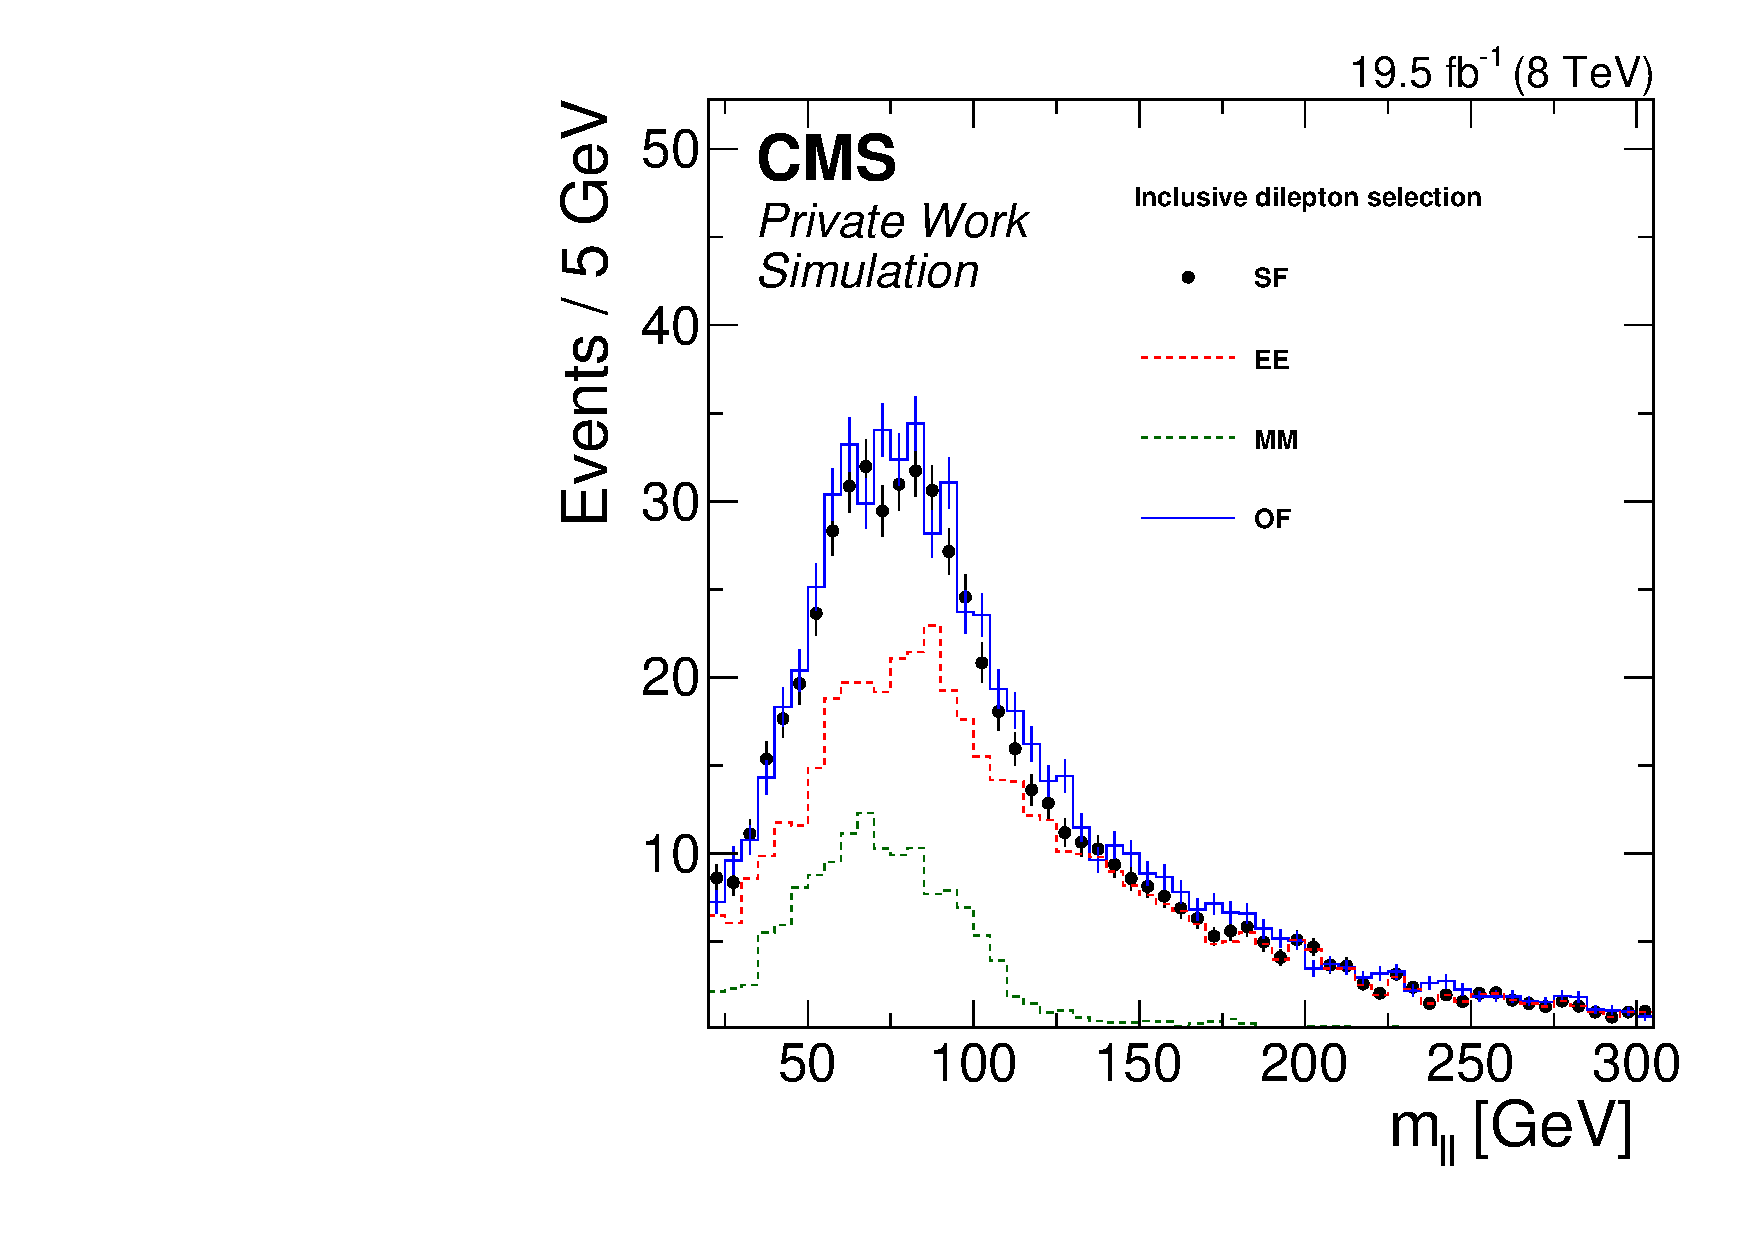
\includegraphics[width=\textwidth]{plots/BG/nonPrompt/nonPromptMC_Inclusive_Full2012_Mll_None.pdf}
\end{minipage}
\begin{minipage}[t]{0.49\textwidth}
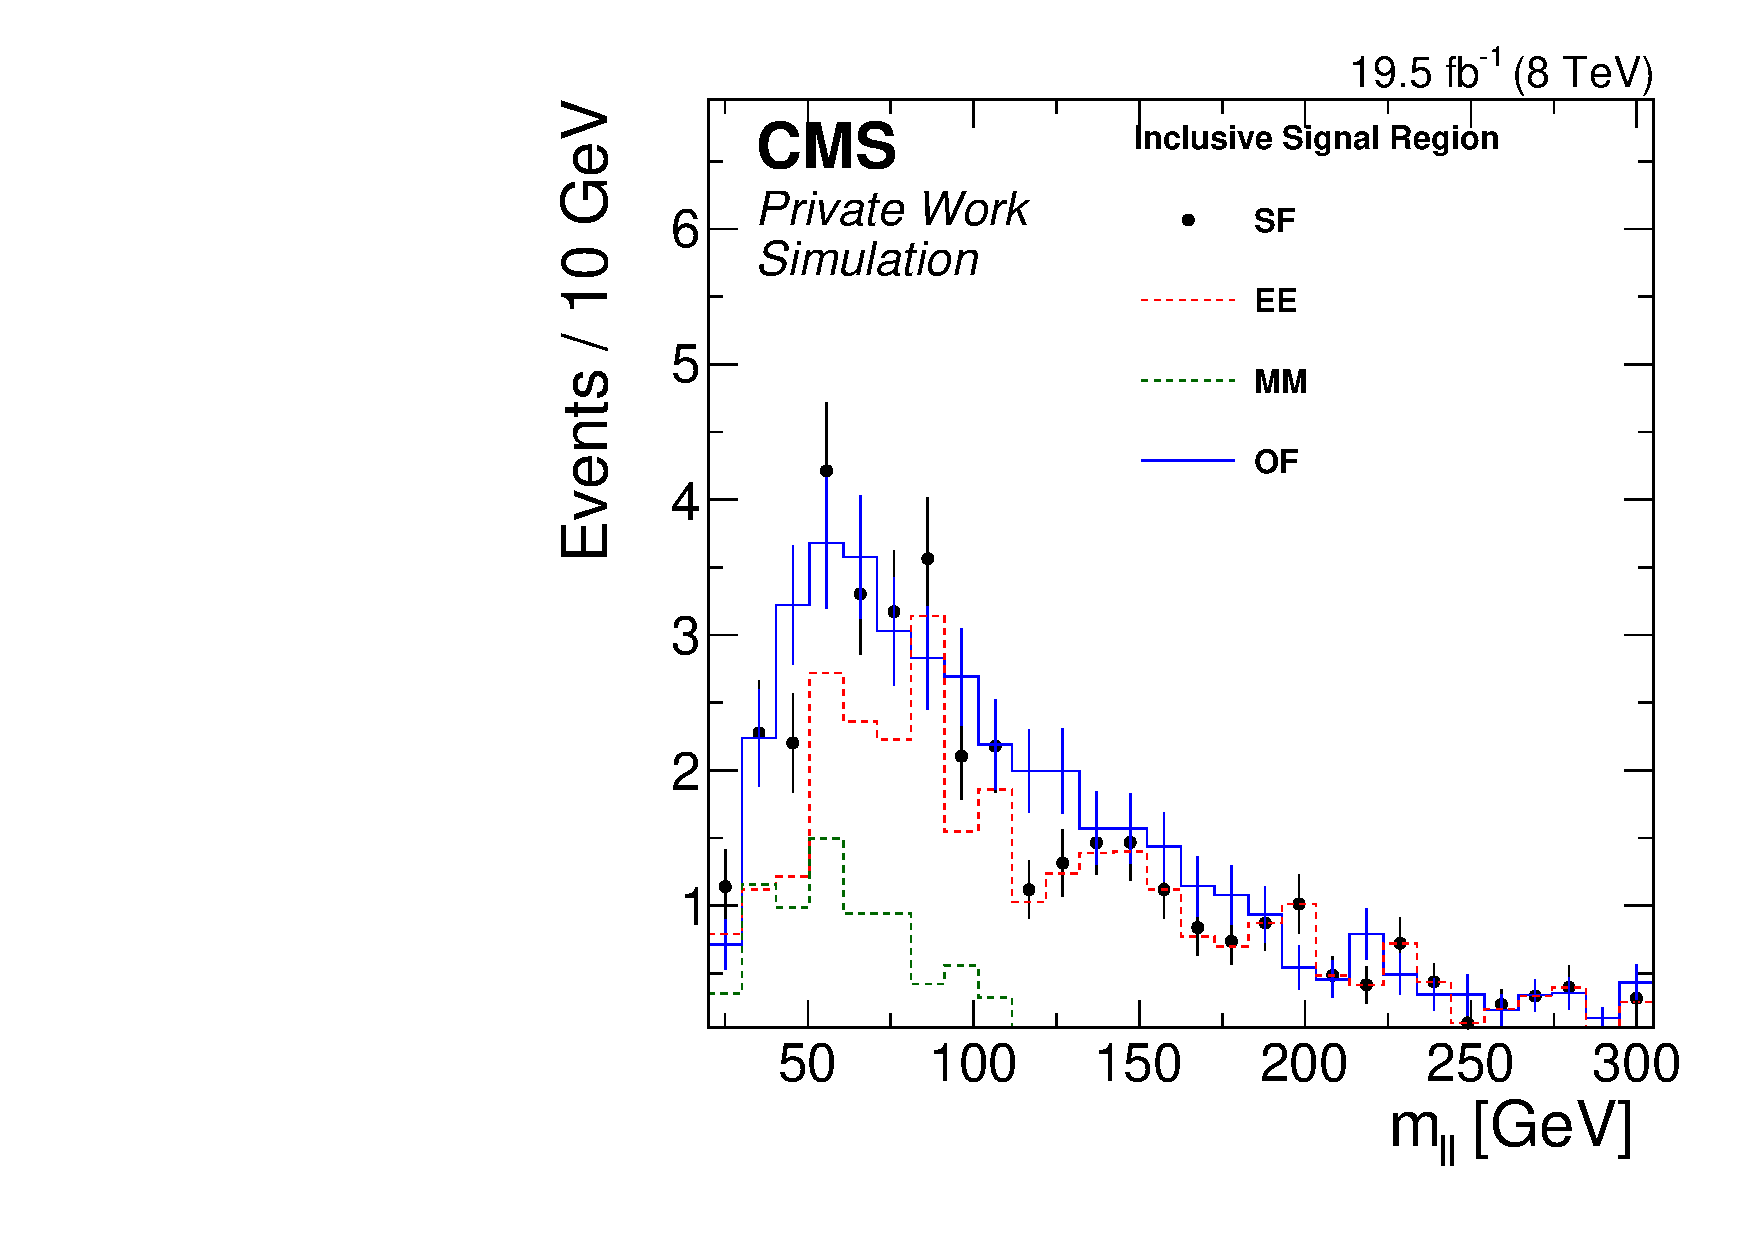
\includegraphics[width=\textwidth]{plots/BG/nonPrompt/nonPromptMC_SignalInclusive_Full2012_Mll_None.pdf}
\end{minipage}
\caption{Distribution of \mll for lepton pairs with at least one non-prompt lepton in simulation for an inclusive dilepton selection (left) and the signal selection (right). The contributions of \EE, \MM, and \EM pairs are shown as red, green, and blue lines, respectively. The combined SF pairs are shown as the black points.}
\label{fig:nonPromptMC}
\end{figure} 
The event yields are summarised in Table~\ref{tab:nonPromptTableMC}. The contribution of non-prompt electrons exceeds that of non-prompt muons. Nevertheless, the event yields for SF and OF lepton pairs are very similar, the OF yields being higher by 5-10\%. This indicates that this type of backgrounds is slightly overpredicted by the estimates for flavour-symmetric backgrounds, which are therefore a conservative estimate for this type of background, at least in simulation. 

\begin{table}[!htbp]
 \renewcommand{\arraystretch}{1.2}
 \begin{center}
  \caption{Number of events with non-prompt leptons in an inclusive dilepton selection, and the central and forward signal regions for \ttbar simulation.}
  \begin{tabular}{l|ccccc}
   \hline
   \hline
                                    & \EE & \MM & SF & \EM    & \Rsfof        \\
   \hline
       Inclusive      &  456.0$\pm$5.2  & 140.3$\pm$3.3 & 596.2$\pm$8.4  & 637.5$\pm$6.3          &  0.94$\pm$0.02    \\
       Signal central      &  20.2$\pm$1.0  & 4.9$\pm$0.6 & 25.0$\pm$1.6  & 26.2$\pm$1.2          &  0.95$\pm$0.07    \\
       Signal forward      &  9.8$\pm$0.7  & 2.8$\pm$0.5 & 12.6$\pm$1.2  & 14.2$\pm$0.9          &  0.89$\pm$0.10    \\

 \end{tabular}
 \label{tab:nonPromptTableMC}
 \end{center}
\end{table}


\paragraph*{Testing the flavour-symmetry of non-prompt leptons on data}
The contribution of non-prompt leptons to the signal selection can be estimated on data from control samples enriched in non-prompt leptons~\cite{fakesnote1,fakesnote2}. These samples are obtained by relaxing the isolation requirements on the leptons from $\frac{\text{Iso}}{\pt} < 0.15$ (``tight'') to $\frac{\text{Iso}}{\pt}<1.0$ (``loose''). In this defintion, every tight lepton is also a loose lepton. The probabilities of a prompt or non-prompt lepton that passes the loose selection to pass also the default tight selection are often referred to as ``fake rate'' $0 < f< 1$ for non-prompt leptons and ``prompt rate'' $0< p< 1$ for prompt leptons. They are calculated as tight-to-loose ratios in two control regions defined below that are enriched in either prompt or non-prompt leptons:
\begin{eqnarray}
f = \frac{N_{\text{tight}}}{N_{\text{loose}}} (\text{non-prompt sample}),\text{                }  p = \frac{N_{\text{tight}}}{N_{\text{loose}}} (\text{prompt sample}).
\end{eqnarray} 
The fake rate $f$ is calculated on an event sample collected with prescaled low-\pt single lepton triggers (see Section~\ref{sec:trigger}). At least one jet with $\pt > \unit{50}{\giga\electronvolt}$ is required. To reject prompt leptons from \Wjets events, \MET and the transverse mass of the lepton-\MET system are both required to be less than $\unit{20}{\giga\electronvolt}$. The resulting fake rates as a function of lepton \pt and $\eta$ are shown in Figure~\ref{fig:fakeRate}. For low \pt, the value for electrons is about 0.25 while for muons it is about 0.07. Dependencies on both \pt and $\eta$ are observed. The fake rate is therefore measured and applied as a function of both variables. The increase for higher \pt is however understood as arising from an increasing contamination from prompt leptons. Therefore, for all leptons with $\unit{\pt > 40}{\giga\electronvolt}$, the values measured for $\unit{35}{\giga\electronvolt} < \pt < \unit{40}{\giga\electronvolt}$ are used.  

\begin{figure}[tbp]
\centering
\begin{minipage}[t]{0.49\textwidth}
  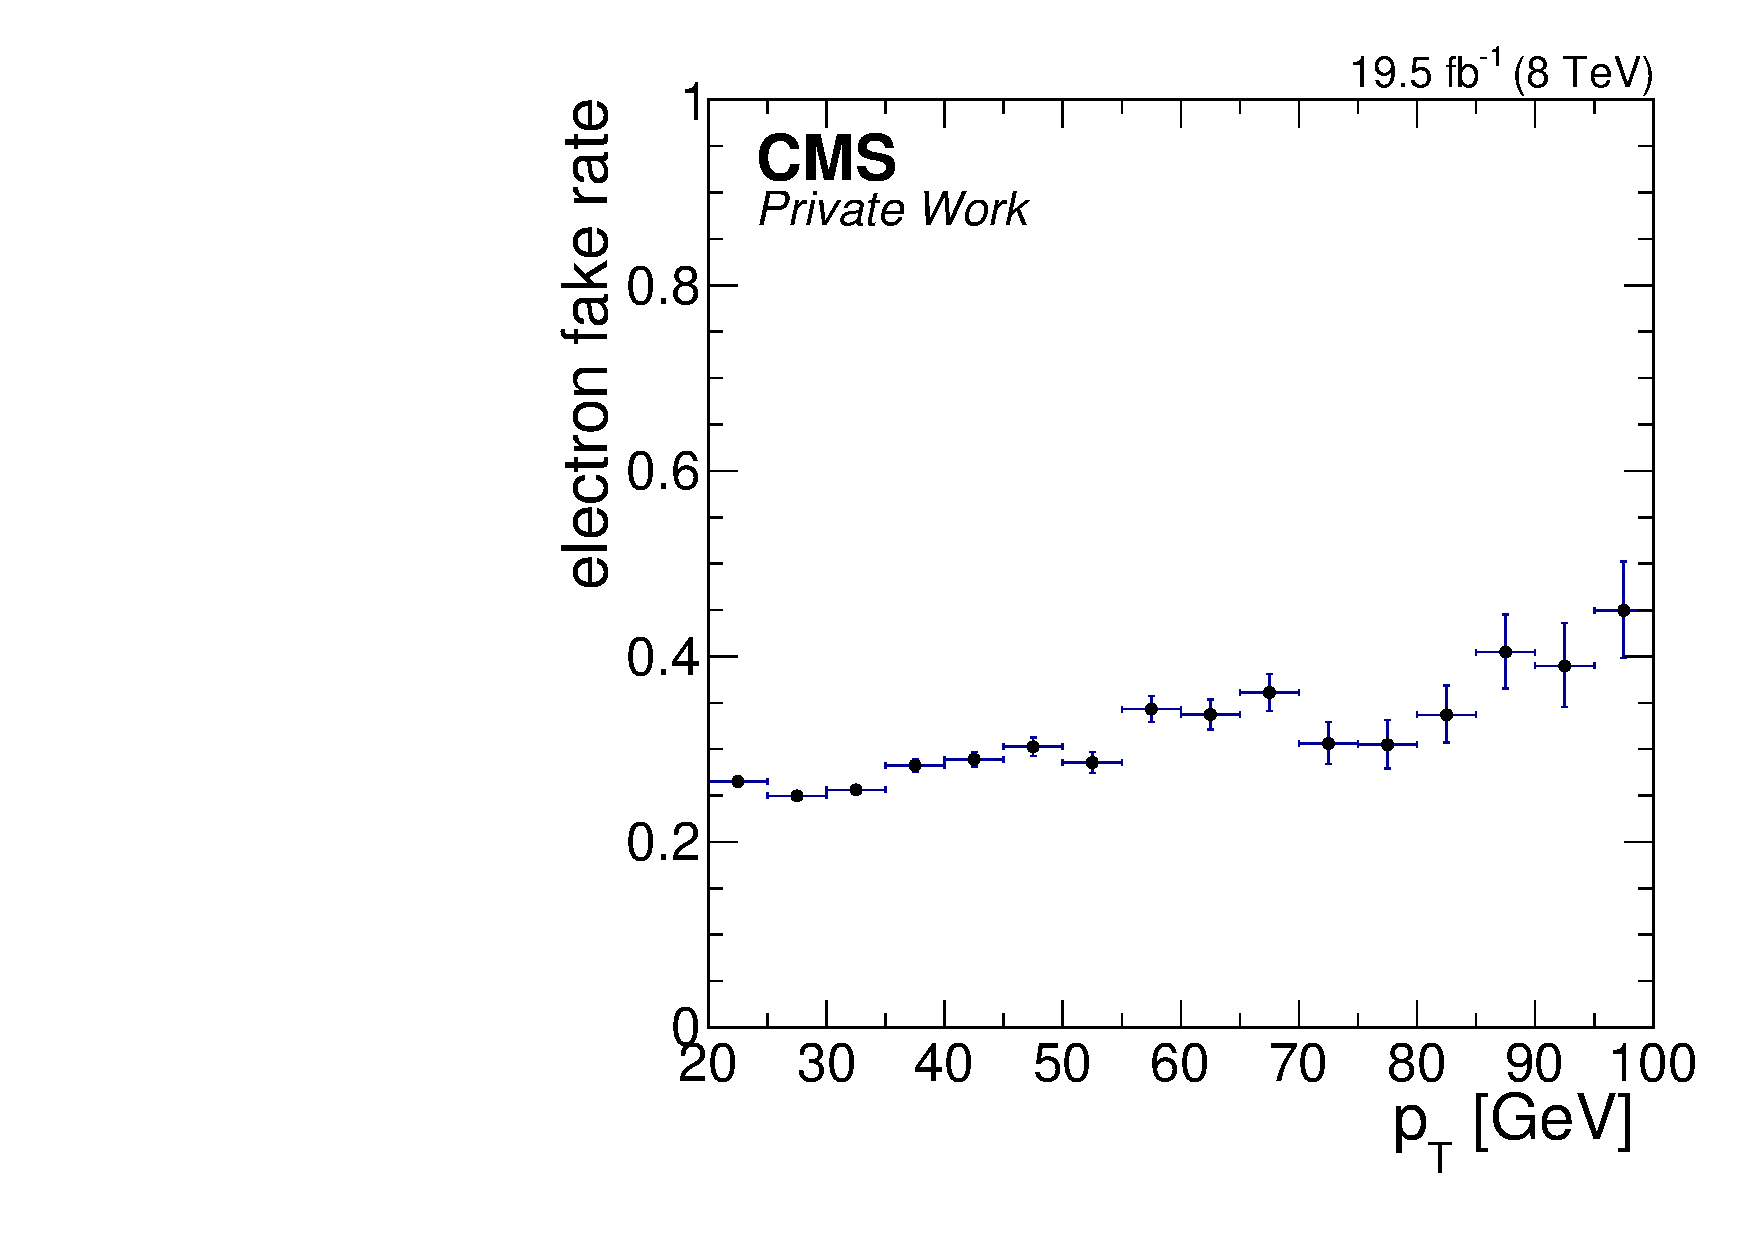
\includegraphics[width=\textwidth]{plots/BG/nonPrompt/fakeRate_ele_Inclusive_Full2012_TrailingPt_range100.pdf}
\end{minipage}
\begin{minipage}[t]{0.49\textwidth}
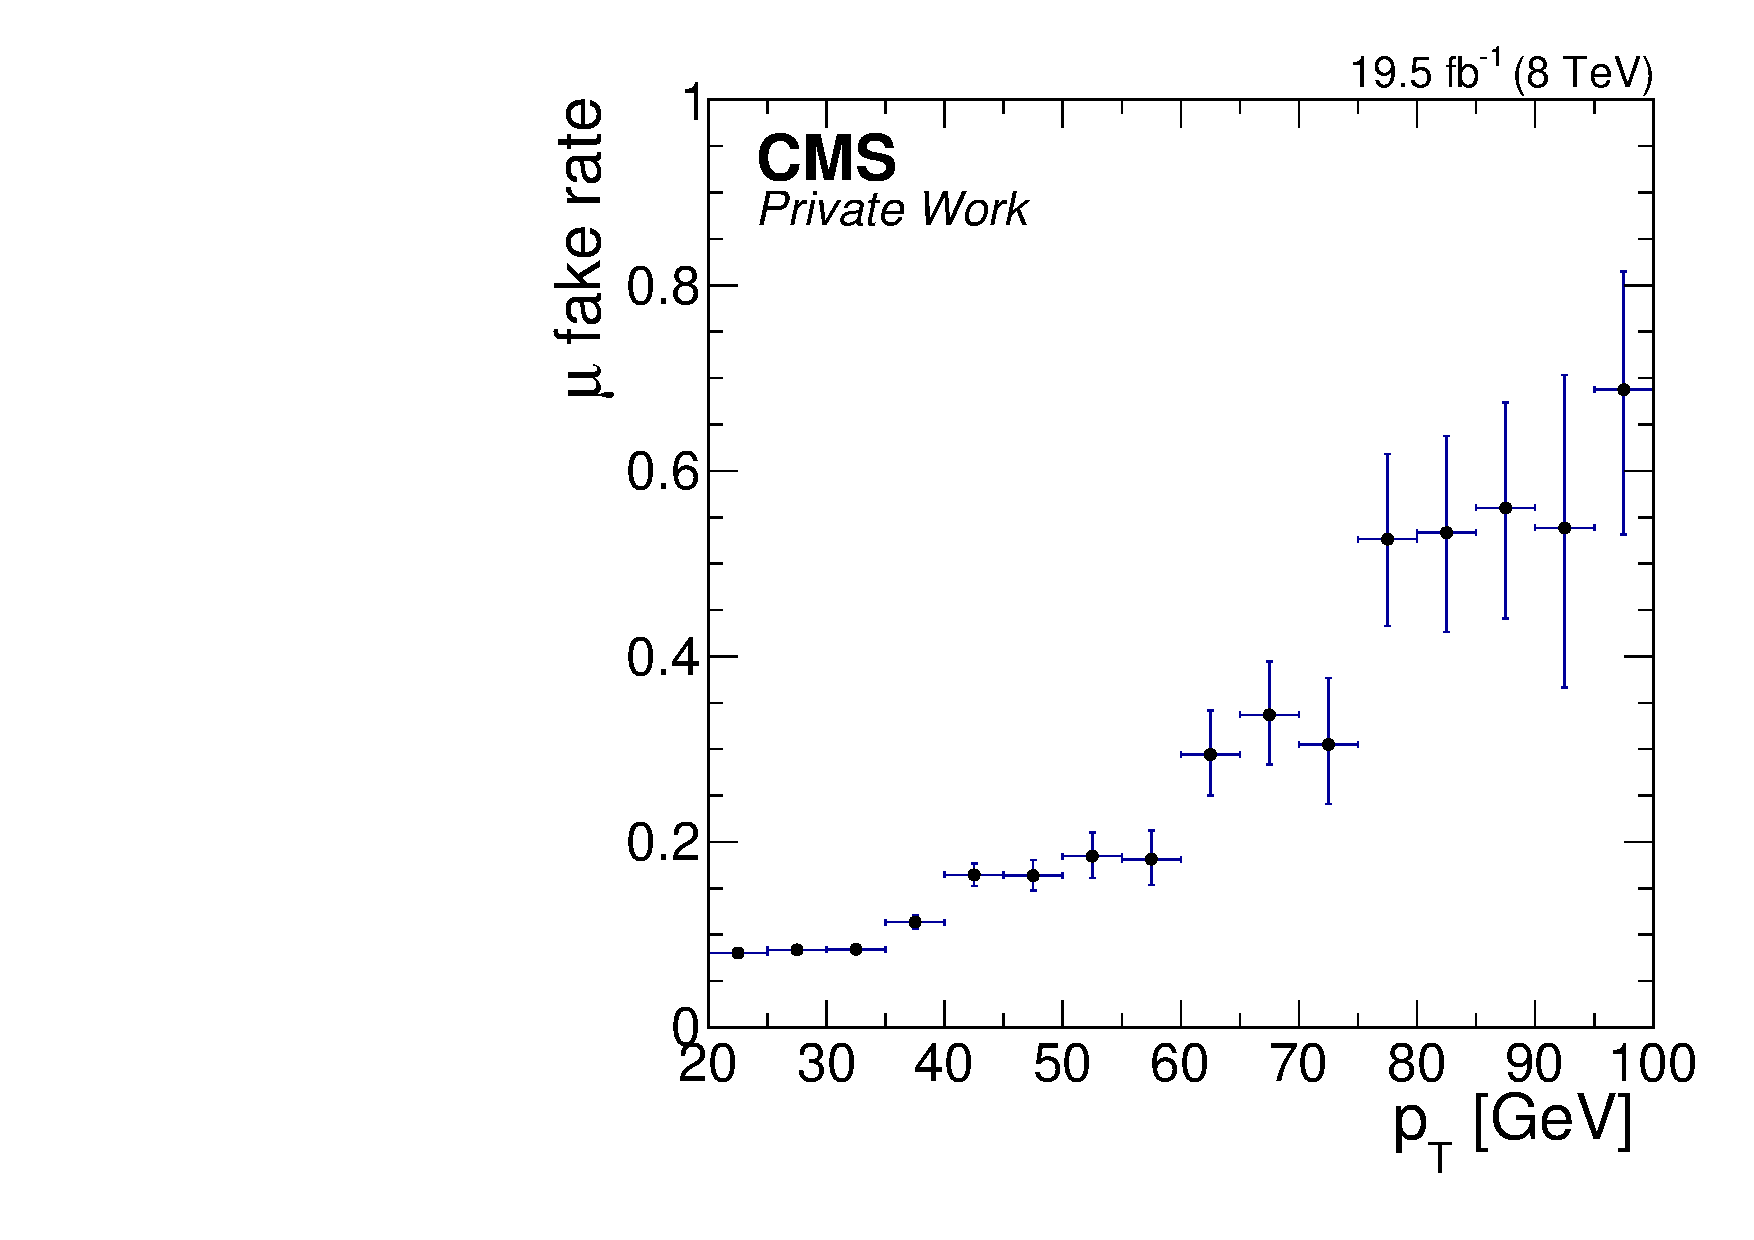
\includegraphics[width=\textwidth]{plots/BG/nonPrompt/fakeRate_mu_Inclusive_Full2012_TrailingPt_range100.pdf}
\end{minipage}
\begin{minipage}[t]{0.49\textwidth}
\includegraphics[width=\textwidth]{plots/BG/nonPrompt/fakeRate_ele_Inclusive_Full2012_TrailingEta_None.pdf}
\end{minipage}
\begin{minipage}[t]{0.49\textwidth}
\includegraphics[width=\textwidth]{plots/BG/nonPrompt/fakeRate_mu_Inclusive_Full2012_TrailingEta_None.pdf}
\end{minipage}
\caption{Measured fake rate for electrons (left) and muons (right) as a function of the \pt (top) and $\eta$ (bottom) of the lepton.}
\label{fig:fakeRate}
\end{figure} 

Similarly, to calculate the prompt rate, a sample enriched in prompt lepton is selected by requiring exactly two reconstructed leptons, of which the leading one is required to be a tight lepton, tagging the event as a \Z boson candidate, while the trailing one is a loose lepton. To further enrich the sample in prompt leptons from \Z boson decays, \mll is required to be within $\unit{15}{\giga\electronvolt}$ of the \Z boson mass and \MET is required to be $\unit{<20}{\giga\electronvolt}$. The resulting prompt ratios $p$ are shown in Figure~\ref{fig:promptRate}. They are again derived as functions of \pt and $\eta$. For low \pt they are about 0.85 for muons and 0.9 for electrons and approach values close to one for $\pt > \unit{60}{\giga\electronvolt}$ for both flavours. The systematic uncertainty assigned to the tight-to-loose ratios in the sources cited above is 50\%. As the definition of loose electrons differs from that used in the analyses referred above and modifications have been made to the definition of the control samples in which the ratios are measured, this number is not directly applicable here. However, the overall normalisation of the non-prompt background is not the focus of this study. Therefore no attempt is made to evaluate this uncertainty for this analysis and no systematic uncertainty is quoted. 

\begin{figure}[tbp]
\centering
\begin{minipage}[t]{0.49\textwidth}
  \includegraphics[width=\textwidth]{plots/BG/nonPrompt/promptRate_ele_Inclusive_Full2012_TrailingPt_range100.pdf}
\end{minipage}
\begin{minipage}[t]{0.49\textwidth}
\includegraphics[width=\textwidth]{plots/BG/nonPrompt/promptRate_mu_Inclusive_Full2012_TrailingPt_range100.pdf}
\end{minipage}
\begin{minipage}[t]{0.49\textwidth}
\includegraphics[width=\textwidth]{plots/BG/nonPrompt/promptRate_ele_Inclusive_Full2012_TrailingEta_None.pdf}
\end{minipage}
\begin{minipage}[t]{0.49\textwidth}
\includegraphics[width=\textwidth]{plots/BG/nonPrompt/promptRate_mu_Inclusive_Full2012_TrailingEta_None.pdf}
\end{minipage}
\caption{Measured prompt rate for electrons (left) and muons (right) as a function of the \pt (top) and $\eta$ (bottom) of the lepton.}


\label{fig:promptRate}
\end{figure} 
Assuming universal fake and tight rates for simplicity, the number of observed events with two tight lepton ($N_{tt}$), one tight and one loose lepton ($N_{tl}$) and two loose leptons ($N_{ll}$) can be expressed in terms of the total numbers of events with two prompt ($N_{pp}^{*}$), one prompt and one non-prompt ($N_{pn}^{*}$), and two non-prompt ($N_{nn}^{*}$): 
\begin{align*}
N_{tt} &= p^2N_{pp}^{*} + pf N_{pn}^{*} + f^2N_{nn}^{*},\\
N_{tl} &= 2p(1-p)N_{pp}^{*} + [f(1-p)+p(-1f)]N_{pn}^{*} + 2f(1-f)N_{nn}^{*},\\
N_{ll} &= (1-p)^2N_{pp}^{*} + (1-p)(1-f)N_{pn}^{*} + (1-f)^2N_{nn}^{*}.
\end{align*}
This can be inverted to obtain expressions for $N_{pp}^{*}$, $N_{pn}^{*}$, and $N_{nn}^{*}$: 
\begin{align*}
N_{pp}^{*} &= \frac{1}{(p-f)^2}[(1-f)^2N_{tt}-f(1-f)N_{tl}+f^2N_{ll}],\\
N_{pn}^{*} &= \frac{1}{(p-f)^2}[-2(1-p)(1-f)N_{tt}-[f(1-p)+p(1-f)]N_{tl}-2fpN_{ll}],\\
N_{nn}^{*} &= \frac{1}{(p-f)^2}[(1-p)^2N_{tt}-p(1-p)N_{tl}+p^2N_{ll}].
\end{align*}
The yields observed inside the tight selection are then given by multiplying with the appropriate tight and fake rates:
\begin{align*}
N_{pp} &= ppN_{pp}^{*},\\
N_{pn} &= pfN_{pn}^{*},\\
N_{nn} &= ffN_{nn}^{*}.\\
\end{align*}
In practice, it has to be considered that the prompt and fake rates depend on the kinematic properties and the flavour of the two leptons. Using the measured fake and prompt rates $f_{1,2}$ and $p_{1,2}$, the contributions of the four possible combinations of prompt and non-prompt leptons (prompt-prompt, prompt-non-prompt, non-prompt-prompt, and non-prompt-non-prompt) are calculated using the following formulas
\begin{eqnarray*}
N_{pp} = \frac{(N_{tt}\cdot(f_1 -1)(f_2-1) + N_{tl}\cdot(f_1 -1)f_2 + N_{lt}\cdot (f_2-1)f_1 + N_{ll}\cdot f_1f_2)p_1p_2}{(f_1-p_1)(f_2-p_2)},\\
N_{pn} = \frac{(N_{tt}\cdot(f_1 -1)(1-p_2) - N_{tl}\cdot(f_1 -1)p_2 + N_{lt}\cdot (1-p_2)f_1 - N_{ll}\cdot f_1p_2)p_1f_2}{(f_1-p_1)(f_2-p_2)},\\
N_{np} = \frac{(N_{tt}\cdot(1 - p_1)(f_2 - 1) + N_{tl}\cdot(1-p_1)f_2 - N_{lt}\cdot (f_2-1)p_1 - N_{ll}\cdot f_2p_1)f_1p_2}{(f_1-p_1)(f_2-p_2)},\\
N_{nn} = \frac{(N_{tt}\cdot(1-p_1)(1-p_2) - N_{tl}\cdot (1-p_1)p_2 - N_{lt}\cdot (1-p_2)p_1 + N_{ll}\cdot p_1p_2)f_1f_2}{(f_1-p_1)(f_2-p_2)}.\\
\end{eqnarray*}
As the fake and prompt rates depend on \pt and $\eta$ of the leptons, in practice each event is assigned a weight based on whether the leptons are tight or loose as a function of their kinematic properties according to the formulas above. The estimates for the number of events are obtained as the sums of these weights. The first index indicates the trailing and the second the leading lepton. The total contribution of non-prompt backgrounds is given by the sum of $N_{pn}$, $N_{np}$, and $N_{nn}$. The resulting estimates in the central and forward signal regions are shown in Table~\ref{tab:nonPromptTable}. 

\begin{table}[!htbp]
 \renewcommand{\arraystretch}{1.2}
 \begin{center}
  \caption{Results of the estimation of backgrounds with non-prompt leptons in the signal region using the tight-to-loose ratios for prompt and non-prompt leptons. The total non-prompt estimate is given by the sum of the contributions for events with one or two non-prompt leptons $N_{pp}$, $N_{np}$, and $N_{pn}$.}
  \begin{tabular}{l|ccccc}

                                    & \EE & \MM & SF & \EM          \\
   \hline
   & \multicolumn{4}{c}{Signal central} \\
   \hline
       $N_{tt}$      &  1257  & 1450 & 2707  & 2326             \\
       $N_{lt}$ + $N_{tl}$      &  247  & 740 & 987  & 812             \\
       $N_{ll}$      &  11  & 114 & 125  & 50             \\

\hline
       Non-prompt estimate      &  44.9$\pm$14.8  & 34.6$\pm$3.8 & 79.6$\pm$18.6  & 86.7$\pm$12.4             \\

\hline
\hline
   
   & \multicolumn{4}{c}{Signal forward} \\
   \hline
       $N_{tt}$      &  405  & 473 & 878  & 827             \\
       $N_{lt}$ + $N_{tl}$      &  130  & 233 & 363  & 234             \\
       $N_{ll}$      &  6  & 38 & 44  & 32             \\

\hline
       Non-prompt estimate      &  27.3$\pm$8.0  & 17.9$\pm$3.5 & 45.1$\pm$11.5  & 43.4$\pm$8.4             \\

 \end{tabular}
 \label{tab:nonPromptTable}
 \end{center}
\end{table}

The contribution of non-prompt leptons is small compared to the total number of tight lepton pairs and the estimates are well compatible between SF and OF events within the statistical uncertainties. This type of backgrounds is therefore accounted for by the background estimates for flavour-symmetric backgrounds.

\section{Drell--Yan backgrounds}
To estimate the contribution of Drell--Yan backgrounds (see Section~\ref{sec:SMBackgrounds}) to the event sample in the signal region, both the Jet-\Z balance (\JZB) and \MET templates methods~\cite{Chatrchyan:2012qka} are used. They are designed to describe the \MET distribution in this category of backgrounds and focus on the description of the on-Z region. The first studies the balance of \Z boson candidates against the jets in the event. In the \MET template method, the \MET distribution of \gjets events are used to estimate that of \zjets events. As the development and application of these methods have not been part of the work covered in this thesis, only a short description will be given. The reported results are those obtained on the first reconstruction of the dataset published in~\cite{Khachatryan:2015lwa}, corrected for slight differences in event kinematics to the reconstruction version used in this analysis. 
\subsection{JZB method}
The \JZB variable is defined as the balance of the \pt of the jets in the event with the \pt of the $\Z\rightarrow \ell^{+}\ell^{-}$ candidate. To avoid biases due to jet selection, \METVec is used as a measure of the hadronic recoil of the \Z boson:
\begin{equation}
\JZB = \abs{ \sum\limits_{\mathrm{jets}}\vec{p}_{\mathrm{T}} } - \abs{ \vec{p}_{\mathrm{T}}^{\text{ }\mathrm{Z}}} \approx \abs{ \vec{E}_{\mathrm{T}}^{\mathrm{miss}} -  \vec{p}_{\mathrm{T}}^{\text{ }\mathrm{ Z}}} - \abs{\vec{p}_{\mathrm{T}}^{\text{ }\mathrm{Z}}} .
\end{equation}
For SM processes such as \zjets, with $\Z \rightarrow \ell^+\ell^-$, where \MET is caused by mismeasurements of the jets, the \JZB distribution is symmetric around 0. For BSM processes, where the \Z boson is produced correlated with invisible particles, the \JZB distribution is expected to be asymmetric, favouring a positive sign especially for large values of \JZB and, by extension, high \MET. Therefore, it is possible to predict the contribution of SM processes containing a \Z boson at high \MET from the events in that region with negative values of \JZB. In both region, backgrounds from flavour-symmetric processes are subtracted from OF events. This results in a final estimate of 
\begin{equation*}
N_{\JZB}^{\text{pred}} = N_{\JZB < 0}+ N_{\JZB > 0}^{\text{pred}} = 2\cdot N_{\JZB < 0} - N_{\JZB < 0}^{OF}\cdot \Rsfof - N_{\JZB > 0}^{OF}\cdot \Rsfof. 
\end{equation*}
 The assumption that the \JZB distribution is symmetric around 0 for SM processes with only instrumental \MET is studied in MC and 20\% systematic uncertainty are assigned~\cite{Khachatryan:2015lwa}.
\subsection{\MET templates method}
The \MET templates method utilises the similarity of \zjets and \gjets events, especially the fact that mismeasurement is the only source of \MET in both cases. Therefore, after corrections for residual kinematic differences, the contribution of \zjets events at high \MET can be estimated from \gjets events passing the same selection. Signals producing both \Z bosons and photons are therefore at least partially included in these estimates. However, this would result in discrepancies between the \JZB and \MET templates results, retaining some sensitivity to this kind of models. The dominant systematic uncertainties are assigned based on tests of the method on simulation and are in the order of 15-100\% for \MET values falling into the signal selection of this analysis. The large uncertainties for higher \MET values are driven by the available number of simulated events to validate the method. 

In contrast to the \JZB method, the \MET templates method does only account for \zjets events. Other backgrounds containing \Z bosons, such as \WZ, \ZZ or more rare SM processes like $t\bar{t}\mathrm{Z}$ or triboson production are estimated from simulation and assigned 50\% uncertainty~\cite{Khachatryan:2015lwa}. The full Drell--Yan prediction from the \MET templates in a given event selection is therefore given by
\begin{equation*}
N_{\MET\text{ templates}}^{\text{pred}} = N_{\gjets}\cdot\text{kinematic corrections} + N_{\text{Diboson, rare SM}}^{\text{MC}} - N_{OF}\cdot \Rsfof. 
\end{equation*}
\subsection{Extrapolation to off-Z regions}
\label{sec:ROutIn}
Both methods described above result in background estimates for the on-\Z region (81\GeV $< \mll < $ 101\GeV). Contributions to the low-mass and high-mass selections from off-shell \Z bosons or the Drell--Yan continuum are estimated by applying an extrapolation factor \Routin to the on-\Z prediction. This approach relies on the assumption that the \mll distribution of Drell--Yan events, and especially the ratio of the contribution on the \Z boson peak to that at lower or higher masses, is the same independent of \MET and \njets. \Routin is measured in the Drell--Yan control region, separately for the low-mass and high-mass region as well as for \EE, \MM, and SF leptons. It is defined as the ratio of the event yield in the mass region in question (\textit{out}) by that in the on-\Z mass region (\textit{in}), after subtraction of the contribution from flavour-symmetric processes from the OF sample:
\begin{equation}
\Routin = \frac{\mathrm{N}_{\mathrm{out}}^{\mathrm{SF}} - \mathrm{N}_{\mathrm{out}}^{\mathrm{OF}}\Rsfof}{ \mathrm{N}_{\mathrm{in}}^{\mathrm{SF}} - \mathrm{N}_{\mathrm{in}}^{\mathrm{OF}}\Rsfof},
\end{equation} 
where the SF can be substituted by \EE or \MM according to the desired lepton flavour. The \mll distribution in the Drell--Yan control region is shown in Figure~\ref{fig:rOutIn}. The resulting values range from about 6-7\% for the low-mass region to 2-3\% for the high-mass region, as summarised in Table~\ref{tab:rOutIn}.
\begin{figure}[htbp]
\centering
\begin{minipage}[t]{0.49\textwidth}
  \includegraphics[width=\textwidth]{plots/BG/rOutIn/rOutIn_SF_DrellYanControlCentral_Full2012.pdf}
\end{minipage}
\begin{minipage}[t]{0.49\textwidth}
\includegraphics[width=\textwidth]{plots/BG/rOutIn/rOutIn_SF_DrellYanControlForward_Full2012.pdf}
\end{minipage}

\caption{The \mll distribution in the Drell--Yan control region in the central (left) and forward (right) dilepton selection. SF data is shown as the black points while OF data is shown as the blue histogram. The black lines indicate the boundaries of the two \textit{out} regions and the dark red lines those of the \textit{in} region.}
\label{fig:rOutIn}
\end{figure} 

\begin{table}[hbtp]
 \renewcommand{\arraystretch}{1.3}
 \setlength{\belowcaptionskip}{6pt}
 \centering
 \caption{
     }
  \label{tab:rOutIn}
\begin{tabular}{l|c|c|c}     
 & $N_{\text{out}}$ & $N_{\text{in}}$ & $ \Routin (SF) \pm \sigma_{stat}$  \\    
\hline
 & \multicolumn{3}{c}{Central} \\
\hline 
 & \multicolumn{3}{c}{Low mass}   \\ 
  Data & 11608.6$\pm$131.7 & 160645.8$\pm$403.9 & 0.072$\pm$0.001$\pm$0.018 \\
 MC & 10725.8$\pm$128.7 & 167291.6$\pm$412.0 & 0.064$\pm$0.001$\pm$0.016 \\

\hline 
& \multicolumn{3}{c}{high Mass} \\ 
\hline
 Data & 3571.3$\pm$91.2 & 160645.8$\pm$403.9 & 0.022$\pm$0.001$\pm$0.006 \\
 MC & 3243.0$\pm$88.9 & 167291.6$\pm$412.0 & 0.019$\pm$0.001$\pm$0.005 \\

 
    \hline 
& \multicolumn{3}{c}{Forward} \\
\hline 
 & \multicolumn{3}{c}{Low mass}   \\ 
  Data & 5657.6$\pm$84.2 & 94407.6$\pm$308.7 & 0.060$\pm$0.001$\pm$0.015 \\
 MC & 5695.8$\pm$85.5 & 103407.4$\pm$323.0 & 0.055$\pm$0.001$\pm$0.014 \\

\hline 
& \multicolumn{3}{c}{high Mass} \\ 
\hline
 Data & 2672.5$\pm$75.8 & 94407.6$\pm$308.7 & 0.028$\pm$0.001$\pm$0.007 \\
 MC & 2459.1$\pm$72.3 & 103407.4$\pm$323.0 & 0.024$\pm$0.001$\pm$0.006 \\


  
\end{tabular}  
\end{table}

The validity of applying the \Routin as measured in the Drell--Yan control region in the signal region is checked by studying the behaviour of the quantity as a function of \MET and \njets. The results for the low-mass selection and the case of SF leptons is shown in Figure~\ref{fig:ROutInDependencies} for both the central and forward lepton selections. In neither selection a dependency on \MET is observed. However, above 70\GeV there is not enough statistics left after subtraction of the flavour-symmetric backgrounds, so it is not possible to judge the behaviour all the way up to the signal region. The value of \Routin clearly increases with the number of jets. As the requirement on \njets is very similar between the Drell--Yan control region and the signal region, the events do not differ much in terms of jet multiplicity and this dependency does not restrict the applicability of the \Routin factors in the signal region. In total, a systematic uncertainty of 25\% is assigned to cover the observed effects. Consistent results are observed also for the high-mass region and for the split into \EE and \MM, as can be seen in Appendix~\ref{app:routin}.

\begin{figure}[htbp]
\centering
\begin{minipage}[t]{0.49\textwidth}
  \includegraphics[width=\textwidth]{plots/BG/rOutIn/rOutInSyst_DrellYanControlCentral_Full2012_MET_LowMass_SF_None.pdf}
\end{minipage}
\begin{minipage}[t]{0.49\textwidth}
\includegraphics[width=\textwidth]{plots/BG/rOutIn/rOutInSyst_DrellYanControlCentral_Full2012_NJets_LowMass_SF_None.pdf}
\end{minipage}
\begin{minipage}[t]{0.49\textwidth}
  \includegraphics[width=\textwidth]{plots/BG/rOutIn/rOutInSyst_DrellYanControlForward_Full2012_MET_LowMass_SF_None.pdf}
\end{minipage}
\begin{minipage}[t]{0.49\textwidth}
\includegraphics[width=\textwidth]{plots/BG/rOutIn/rOutInSyst_DrellYanControlForward_Full2012_NJets_LowMass_SF_None.pdf}
\end{minipage}
\caption{Dependencies of \Routin for the low-mass region on \MET (left) and \njets (right) for the central (top) and forward (bottom) lepton selection. The results on data are shown in black. The central value is shown as a black dashed line while the systematic uncertainty is shown as an orange band.}
\label{fig:ROutInDependencies}
\end{figure} 


\subsection{Resulting background prediction}
The predictions for the on-\Z region from the \JZB and \MET templates methods agree within their uncertainties, as can be seen in Table~\ref{tab:dyResults}. As for the \Rsfof factor, a weighted average is used to combine the two estimates. The results of both methods as well as the combination are shown in Table~\ref{tab:dyResults}. Shown are also the \Routin values and the resulting estimates for the low- and high-mass regions. In this analysis a different reconstruction version of the data is used, compared to the one used in~\cite{Khachatryan:2015lwa}. Therefore, the on-\Z predictions, which are taken from the published result, are scaled by 1.03$\pm$0.03 to take into account a slight increase in jet multiplicity observed in the present dataset.

\begin{table}[!htbp]
 \renewcommand{\arraystretch}{1.2}
 \begin{center}
  \caption{Estimate of the \Z background yields in the \Z peak region and extrapolation to the signal mass region for the full dataset.}
  \begin{tabular}{l|cc|c|}
   \hline
   \hline
                                    & \multicolumn{3}{c|}{\central}            \\
                                    & \EE                   & \MM                   & SF          \\
   \hline
   \Z bkgd estimate (\JZB)                  & $57.9\pm13.8\pm10.1$   & $46.1\pm13.8\pm8.0$          &    $104\pm21\pm18$  \\
   
   \Z bkgd estimate (\MET templates) & $63.2\pm 4.3\pm 15.3$    & $69.5\pm 4.0\pm 16.9$       &    $133\pm7\pm32$  \\
   \Z bkgd estimate (Combined)         & $60.7\pm 11.6$                & $56.8\pm 11.7$                   &    $116\pm21$  \\
   \hline
       \Routin low-Mass       &  0.069$\pm$0.001$\pm$0.017                   & 0.075$\pm$0.001$\pm$0.019            &  0.072$\pm$0.001$\pm$0.018    \\
 
   \hline
     low-Mass estimate    & 4.3$\pm$1.3        & 4.4$\pm$1.4  &  8.6$\pm$2.7 \\

   \hline
       \Routin high-Mass       &  0.025$\pm$0.001$\pm$0.006                   & 0.020$\pm$0.001$\pm$0.005            &  0.022$\pm$0.001$\pm$0.006    \\
 
   \hline
     high-Mass estimate    & 1.5$\pm$0.5        & 1.2$\pm$0.4  &  2.7$\pm$0.8 \\
  
   \hline
                                    & \multicolumn{3}{c|}{\forward} \\
                                    & \EE                  & \MM                        & SF \\
   \hline
   \Z bkgd estimate (\JZB)                   & $15.6\pm 8.3\pm 2.9$ & $13.8 \pm 8.3\pm 2.8$       & $29\pm11\pm6$ \\
   \Z bkgd estimate (MET templates)          & $24.4\pm 1.8\pm 6.0$ & $32.3\pm 2.2\pm 7.9$       & $56.9\pm3.6\pm14.0$ \\
   \Z bkgd estimate (Combined)          & $21\pm 5$        & $25\pm 6$             & $42\pm 9$  \\

   \hline
       \Routin low-Mass       &  0.055$\pm$0.001$\pm$0.014                   & 0.064$\pm$0.001$\pm$0.016            &  0.060$\pm$0.001$\pm$0.015    \\

   \hline
     low-Mass estimate    & 1.2$\pm$0.4        & 1.6$\pm$0.6  &  2.6$\pm$0.8 \\


   \hline
       \Routin high-Mass       &  0.031$\pm$0.001$\pm$0.008                   & 0.026$\pm$0.001$\pm$0.007            &  0.028$\pm$0.001$\pm$0.007    \\

   \hline
     high-Mass estimate    & 0.7$\pm$0.2        & 0.7$\pm$0.2  &  1.2$\pm$0.4 \\

   \hline
   \hline
 \end{tabular}
 \label{tab:dyResults}
 \end{center}
\end{table}






\chapter{Results}
\label{sec:counting}
In the counting experiment approach, the observed yield of SF events is compared to the combined background estimates from flavour-symmetric and Drell--Yan backgrounds in the six region defined in \mll and lepton $|\eta|$. Here, the results are presented and further investigations into their properties are discussed. Also the implications of these results on the the simplified models discussed in section~\ref{sec:models} is examined.  
\section{Results and further studies}

\label{sec:candcresults}
The distribution of the dilepton invariant mass in the central and forward signal regions are shown in Figure~\ref{fig:resultsCC}. The resulting event yields are compared to the expectation from SM backgrounds in Table~\ref{tab:METresults2012}. A maximum likelihood fit is performed in each region to find the best estimator for the difference of expected and observed yield. The significances of deviations of this difference from zero are evaluated using the profile likelihood ratio of the signal and signal plus background hypotheses~\cite{HiggsTool1}. In general, the observed data is in agreement with the background estimation within about one standard deviation, except for the low-mass region for central leptons. Here, the observed yield exceeds the expectation by $109\pm48$ events. The size of this excess corresponds to a significance of 2.2~$\sigma$.  
\begin{figure}[htbp]
\centering
\begin{minipage}[t]{0.49\textwidth}
  \includegraphics[width=\textwidth]{plots/results/mllResult_SignalCentral_Full2012_SF.pdf}
\end{minipage}
\begin{minipage}[t]{0.49\textwidth}
\includegraphics[width=\textwidth]{plots/results/mllResult_SignalForward_Full2012_SF.pdf}
\end{minipage}

\caption{Distribution of \mll in the signal region for the central (left) and forward (right) dilepton selection. The data is shown as black dots, while the total background prediction from data is shown as a blue histogram. The blue error bars indicate the combined statistical and systematic background uncertainty in each bin. The contribution from Drell--Yan backgrounds is shown as a green histogram. The dashed lines indicates the boundaries of the three mass bins. Beneath the plot the ratio of data to the background prediction is shown. The error bars include the statistical uncertainties of data and background, while the blue band indicates the systematic uncertainties on the background. }
\label{fig:resultsCC}
\end{figure} 


\begin{table}[btp]
 \renewcommand{\arraystretch}{1.3}
 \setlength{\belowcaptionskip}{6pt}
 \scriptsize
 \centering
 \caption{Results of the counting experiment in the six signal regions.
     The statistical and systematic uncertainties are added in quadrature, except for the flavor-symmetric backgrounds. The presented differences between the observed and estimated yields are obtained with a maximum likelihood fit (see text).    Low-mass refers to $20\GeV < \mll < 70$\GeV, on-\Z to  $81\GeV < \mll < 101$\GeV, and high-mass to $\mll > 120$\GeV.
     }
  \label{tab:METresults2012}
  \begin{tabular}{l| cc | cc | cc}

    							& \multicolumn{2}{c}{low-mass} & \multicolumn{2}{c}{on-\Z} & \multicolumn{2}{c}{high-mass} \\ 

    \hline
                                &  Central        & Forward  &  Central  & Forward   &  Central        & Forward \\ 

    \hline
        Observed       &  865                   & 154              &  494            &  176       &   849           &   381    \\

    \hline
        Flav.-sym.    & $746\pm27\pm26$        & $144\pm12\pm7$  &  $368\pm19\pm13$ & $137\pm11\pm7$ & $789\pm28\pm28$ & $411\pm20\pm21$ \\

            Drell--Yan          & $8.6\pm2.7$            & $2.6\pm0.8$      & $119\pm21$ & $43\pm9$ & $2.7\pm0.8$ & $1.2\pm0.4$ \\

    \hline
            Total est.          & $755\pm38$            & $147\pm14$      & $488\pm31$ & $180\pm16$ & $792\pm39$ & $413\pm30$ \\

    \hline
         Obs. - est.  & $109\pm48$      & $7\pm19$ & $6\pm38 $ & $-5\pm21$ & $57\pm50$ & $-32\pm37 $ \\ 

    \hline
   Significance      & 2.2~$\sigma$    &  0.4~$\sigma$  & 0.1~$\sigma$ & $<$0.1~$\sigma$ & 1.1~$\sigma$ & $<$0.1~$\sigma$ \\ 


  \end{tabular}
\end{table}



In the Tables~\ref{tab:METresults2012EE} and~\ref{tab:METresults2012MM}, the results are shown separately for \EE and \MM events. As expected from the fact that \rmue is larger than one, the yields in the \MM channel are slightly larger than in the \EE channel. For the flavour-symmetric backgrounds, and therefore also for the total background estimates and the difference of observation and estimation, the yields in the \EE and \MM channels do not exactly add up to those in the combined SF channel presented in Table~\ref{tab:METresults2012}. This is caused by the the weighted average of the two methods to determine the correction factors used to translate from OF into the different SF channels, which is calculated separately for \Rsfof, \Reeof, and \Rmmof, as discussed in Section~\ref{sec:combinedRSFOF}. Comparing the two channels, consistent results are observed between them, except for the slight excess in the high-mass central region, which is driven dominantly from \EE events. Especially for the larger excess in the low-mass central region, the observation agrees with the expected behaviour of the different flavours. The signal yields of $47\pm25$ and $67\pm29$ in the \EE and \MM channels correspond to a value of \rmue for this hypothetical signal of $1.19\pm0.41$, in good agreement with the value of $1.09\pm0.11$ measured in the Drell--Yan control region (see Section~\ref{sec:rmue}).

\begin{table}[hbtp]
 \renewcommand{\arraystretch}{1.3}
 \setlength{\belowcaptionskip}{6pt}
 \scriptsize
 \centering
 \caption{Results of the counting experiment for \EE events only.
     The statistical and systematic uncertainties are added in quadrature, except for the flavor-symmetric backgrounds. The presented differences between the observed and estimated yields are obtained with a maximum likelihood fit (see text).    Low-mass refers to $20 < \mll < 70$\GeV, on-\Z to  $81 < \mll < 101$\GeV, and high-mass to $\mll > 120$\GeV.
     }
  \label{tab:METresults2012EE}
  \begin{tabular}{l| cc | cc | cc}

    							& \multicolumn{2}{c}{low-mass} & \multicolumn{2}{c}{on-\Z} & \multicolumn{2}{c}{high-mass} \\ 

    \hline
                                &  Central        & Forward  &  Central  & Forward   &  Central        & Forward \\ 

    \hline
        Observed       &  389                   & 53              &  232            &  86       &   401           &   195    \\

    \hline
        Flav.-sym.    & $337\pm12\pm19$        & $61\pm5\pm6$  &  $166\pm8\pm9$ & $58\pm5\pm5$ & $357\pm12\pm21$ & $175\pm8\pm17$ \\

            Drell--Yan          & $4.3\pm1.3$            & $1.2\pm0.4$      & $62\pm11$ & $21\pm5$ & $1.5\pm0.5$ & $0.7\pm0.2$ \\

    \hline
            Total est.          & $342\pm23$            & $62\pm8$      & $229\pm17$ & $79\pm9$ & $358\pm24$ & $175\pm19$ \\

    \hline
         Obs. - est.  & $47\pm25$      & $-10\pm9$ & $3\pm21 $ & $6\pm12$ & $42\pm26$ & $19\pm18 $ \\ 

    \hline
   Significance      & 1.9~$\sigma$    &  $<$0.1~$\sigma$  & 0.1~$\sigma$ & 0.5~$\sigma$ & 1.7~$\sigma$ & 1.1~$\sigma$ \\ 


  \end{tabular}
\end{table}





\begin{table}[hbtp]
 \renewcommand{\arraystretch}{1.3}
 \setlength{\belowcaptionskip}{6pt}
 \scriptsize
 \centering
 \caption{Results of the counting experiment for \MM events only.
     The statistical and systematic uncertainties are added in quadrature, except for the flavor-symmetric backgrounds.
     Low-mass refers to $20 < \mll < 70$\GeV, on-\Z to  $81 < \mll < 101$\GeV and high-mass to $\mll > 120$\GeV.
     }
  \label{tab:METresults2012MM}
  \begin{tabular}{l| cc | cc | cc}

    							& \multicolumn{2}{c}{low-mass} & \multicolumn{2}{c}{on-\Z} & \multicolumn{2}{c}{high-mass} \\ 

    \hline
                                &  Central        & Forward  &  Central  & Forward   &  Central        & Forward \\ 

    \hline
        Observed       &  476                   & 101              &  262            &  90       &   448           &   186    \\

    \hline
        Flavor-symmetric    & $405\pm14\pm21$        & $79\pm6\pm6$  &  $200\pm10\pm10$ & $74\pm6\pm6$ & $428\pm15\pm23$ & $224\pm11\pm19$ \\

            Drell--Yan          & $4.4\pm1.4$            & $1.6\pm0.6$      & $58\pm10$ & $25\pm6$ & $1.2\pm0.4$ & $0.7\pm0.2$ \\

    \hline
            Total estimated          & $409\pm26$            & $80\pm9$      & $258\pm18$ & $100\pm11$ & $429\pm27$ & $225\pm22$ \\

    \hline
         Observed - estimated  & $67^{+29}_{-29}$      & $20^{+13}_{-13}$ & $3^{+22}_{-23} $ & $-11^{+13}_{-13}$ & $19^{+29}_{-29}$ & $-40^{+21}_{-21} $ \\ 

    \hline
   Significance      & 2.3~$\sigma$    &  1.6~$\sigma$  & 0.2~$\sigma$ & $<$0.1~$\sigma$ & 0.6~$\sigma$ & $<$0.1~$\sigma$ \\ 


  \end{tabular}
\end{table}





\subsection*{Investigating the low-mass central region}
While a significance of $2.2\sigma$ is no clear indication for the presence of new physics, more detailed studies into the properties of this excess are conducted. 

The development of the excess during the data taking period in 2012 is shown on the left side of Figure~\ref{fig:timeDependece}, while the right side shows the low-mass forward region for comparison. The data sample is split into 10 bins, each corresponding to 2\,$fb^{-1}$ within 1\%, except for the last which corresponds to only  about 1.5\,$fb^{-1}$. For each of these bins the observed SF yield and the prediction for flavour-symmetric backgrounds from OF is shown, together with the difference of the two. The very small contribution from Drell--Yan backgrounds of typically less than 1 event per bin is neglected in this representation of the result. For the first four bins, corresponding to the first 8\,$fb^{-1}$ of data collected in 2012, the SF yield is significantly higher than the prediction from OF. This effect diminishes in the fifth bin, where the SF yield decreases and the prediction from OF increases. In the following five bins, representing the second half of the data sample, good agreement is observed between the observed SF yield and the prediction from OF. This change in behaviour between the two halves is caused in roughly equal manner by a decrease in the observed SF yield and an increase in the observed OF yield per bin. In contrast to this observations, the SF yield and the background prediction are compatible within uncertainties for all bins in the low-mass forward region. The difference between the two therefore fluctuates around zero.

\begin{figure}[htbp]
\centering
\begin{minipage}[t]{0.49\textwidth}
  \includegraphics[width=\textwidth]{plots/results/YieldvsLumi_Bins_SignalCentral_Mll_edgeMassFull2012.pdf}
\end{minipage}
\begin{minipage}[t]{0.49\textwidth}
\includegraphics[width=\textwidth]{plots/results/YieldvsLumi_Bins_SignalForward_Mll_edgeMassFull2012.pdf}
\end{minipage}

\caption{Observed SF yields and background prediction from OF as well as the difference of these two in the low-mass central (left) and forward (right) signal region in 10 bins of roughly equal integrated luminosity. Non-flavour-symmetric backgrounds are not included in this representation of the result.}
\label{fig:timeDependece}
\end{figure}

To get a clearer picture of the properties of the excess and also to check for some of the more obvious possible systematic effects that might cause it, the counting experiment in the low-mass central region is repeated several times, varying the selection requirements. The results are shown in Table~\ref{tab:CountingCrosschecks}. As no Drell-Yan prediction for the on-\Z region is available for the different configurations, the observed yield is extrapolated into the low-mass region after subtraction of flavour-symmetric background using the prediction from OF. For all these cross-checks presented here one has to keep in mind that for the background prediction from OF the \Rsfof factor derived for the default selection is used.

As the signal region is dominated by events containing b-tagged jets, it seems natural to test the excess for its b-tag content. Splitting the data sample into events with at least one and those without a b-tag, it is evident that, while constituting about 23\% of the total yield, less than 10\% of the excess is located in events without a b-tagged jet. 

In addition to the default selection of $\pt > \unit{20}{\giga\electronvolt}$, four other configurations for the lepton \pt requirement are tested. Three of them feature asymmetric cuts on the \pt of the leading and trailing lepton. The selection of $\pt > 20(10)$ and $ \pt > 30(10)\GeV$ extend the acceptance of the analysis to lower trailing lepton \pt. For both of these selections, an increased signal yield is observed. On the other hand, raising the trailing \pt threshold to 30\GeV disproportionally reduces the observed excess, retaining only about 13\% of the excess yield compared to 23\% of the overall event yield. 

Although it has already been established in Section~\ref{sec:validation} that non-prompt leptons only account for a small part of the selected data sample and are also fully flavour-symmetric, the counting experiment is repeated with significantly tighter isolation requirements. The relative isolation is required to be smaller than 5\%, reducing the size of the selected sample by about one third. The number of observed signal events is reduced by almost exactly the same amount. This further increases the confidence that the observed effect is due to prompt lepton production.

To test for a possible pileup dependence of the observed effect, the sample is split into three subsets of similar size depending on the number of reconstructed vertices. The events are categorised as either low-pileup ($N_{\mathrm{vtx}} < $13), mid-pileup (13 $\leq N_{\mathrm{vtx}} <$ 17) or high-pileup ($N_{\mathrm{vtx}} \geq $17). The excess is observed consistently in all three subsets, excluding a possible pileup dependence of excess. 

Three additional \MET reconstructions are tested. TC \MET and type-I corrected PF \MET have been described in Section~\ref{sec:PF}. In addition to these general algorithms, an analysis-specific definition of missing $H_{\mathrm{T}}$ is used, which is calculated using only selected jets and leptons. It is defined as the absolute value of the negative vector sum of the the transverse momenta of these objects: 
\begin{equation*}
H_{\mathrm{T}}^{\mathrm{miss}} = | -(\sum\limits_{\mathrm{jets}}\vec{p}_{\mathrm{T}} + \sum\limits_{\mathrm{leptons}}\vec{p}_{\mathrm{T}}) |.
\end{equation*}
The signal region requirements of $\unit{100}{\giga\electronvolt}$ and $\unit{150}{\giga\electronvolt}$, depending on \njets, are applied for each of these \MET values.  Both the use of type-I corrected PF \MET and missing $H_{\mathrm{T}}$ lead to higher event yields in the signal region. Judging by the size of the Drell--Yan background, TC \MET and $H_{\mathrm{T}}^{\mathrm{miss}}$ have significantly worse \MET resolution compared to both types of PF \MET. The excess is present in all three cases and is therefore not likely to be caused by a faulty \MET reconstruction. 

Separating the data sample into events with low \HT ($\unit{100}{\giga\electronvolt} < \HT <\unit{300}{\giga\electronvolt}$) and high \HT ($\HT > \unit{300}{\giga\electronvolt}$) creates two subsets of roughly the same size. The excess is present in both subsets with similar strength. 
 


\begin{table}[hbtp]
 \renewcommand{\arraystretch}{1.3}
 \setlength{\belowcaptionskip}{6pt}
 \centering
 \caption{Results of the counting experiment in the low-mass central signal region for different variations of the event selection. The observed event yield in SF events is compared with the combined estimate from flavour-symmetric and Drell--Yan backgrounds. The estimate for the Drell--Yan backgrounds is obtained by extrapolating the event yield in the on-Z signal region after subtraction of flavour-symmetric backgrounds to the low-mass region using the \Routin factor.}
  \label{tab:CountingCrosschecks}
  \begin{tabular}{l|c|c|c|c}
                                &  SF        & Flavour-symmetric  &  Drell--Yan  & Observed - Estimates \\ 

    \hline
    \hline
 & \multicolumn{4}{c}{b-tagging}\\ 
\hline 
        no b-tags       &  202                   & 188.5$\pm$15.4              &  7.1$\pm$2.5            &  6.3$\pm$21.1 \\
        $\geq$ 1 b-tags       &  663                   & 558.4$\pm$31.0              &  1.9$\pm$0.7            &  102.7$\pm$40.3 \\
\hline 
 & \multicolumn{4}{c}{lepton \pt requirement} \\ 
\hline 
        \pt > 20(10)\GeV       &  1474                   & 1290.2$\pm$58.6              &  11.4$\pm$4.1            &  172.5$\pm$70.1 \\
        \pt > 30(10)\GeV       &  1262                   & 1114.8$\pm$52.1              &  11.3$\pm$4.1            &  135.9$\pm$63.2 \\
        \pt > 30(20)\GeV       &  761                   & 674.0$\pm$35.5              &  9.0$\pm$3.3            &  78.0$\pm$45.1 \\
        \pt > 30\GeV       &  296                   & 275.7$\pm$19.4              &  6.5$\pm$2.3            &  13.8$\pm$26.0 \\
\hline 
 & \multicolumn{4}{c}{tight lepton isolation} \\ 
\hline 
        rel. isolation < 0.05       &  572                   & 491.5$\pm$28.4              &  7.1$\pm$2.6            &  73.3$\pm$37.2 \\
\hline 
 & \multicolumn{4}{c}{pileup} \\ 
\hline 
        $N_{\text{vtx}} <$ 13       &  332                   & 289.9$\pm$20.0              &  3.3$\pm$1.2            &  38.8$\pm$27.1 \\
        13 $\leq N_{\text{vtx}}$ < 17       &  242                   & 212.8$\pm$16.5              &  0.9$\pm$0.3            &  28.3$\pm$22.7 \\
        $N_{\text{vtx}} \geq$ 17       &  291                   & 244.2$\pm$18.0              &  4.8$\pm$1.7            &  41.9$\pm$24.8 \\
\hline 
 & \multicolumn{4}{c}{\MET reconstructions}\\
\hline 
        type I corrected PF \MET       &  1034                   & 923.3$\pm$45.0              &  9.4$\pm$3.4            &  101.3$\pm$55.4 \\
        track corrected \MET       &  850                   & 702.3$\pm$36.6              &  26.3$\pm$9.4            &  121.3$\pm$47.7 \\
        missing $H_{\mathrm{T}}$       &  1171                   & 942.5$\pm$45.7              &  50.8$\pm$18.1            &  177.6$\pm$59.9 \\
\hline 
 & \multicolumn{4}{c}{$H_{\mathrm{T}}$}\\
\hline 
        100\GeV $< H_{\mathrm{T}} < $ 300\GeV        &  455                   & 401.3$\pm$24.7              &  1.4$\pm$0.5            &  52.3$\pm$32.7 \\
        $H_{\mathrm{T}} > $ 300\GeV        &  410                   & 344.6$\pm$22.4              &  7.5$\pm$2.7            &  57.9$\pm$30.3 \\
\hline 


  \end{tabular}
\end{table}




The distributions of several observables in the low-mass signal region is shown in Figure~\ref{fig:dependencies}. Each time the observed data is compared to the prediction from OF events. The contribution from Drell--Yan backgrounds is neglected. The excess is located predominantly in events with one or two b-tagged jets, but no excess is observed for higher b-tag multiplicities. Furthermore, it is located almost inclusively in events with three jets. It is present in events with a \pt of the leading lepton of up to $\unit{60}{\giga\electronvolt}$. For events with a trailing lepton \pt above $\unit{25}{\giga\electronvolt}$, only a small deviation from the expectation is observed. The excess seems to favour low values of \MET and is roughly uniformly distributed in \HT. 

In all performed studies, no evidence for systematic effects causing the observed excess is found. The two major distinguishing features of the events causing the deviation are the presence of at least one b-tagged jet and trailing leptons with very low \pt. In general, no features distinguishing the events in the excess from the dominant \ttbar background are observed in any of the performed studies. 

\begin{figure}[htbp]
\centering
\begin{minipage}[t]{0.49\textwidth}
  \includegraphics[width=\textwidth]{plots/results/rSFOFDependencies/rSFOFDependency_SignalCentral_NBJets_Full2012_SF_lowMass.pdf}
\end{minipage}
\begin{minipage}[t]{0.49\textwidth}
\includegraphics[width=\textwidth]{plots/results/rSFOFDependencies/rSFOFDependency_SignalCentral_NJets_Full2012_SF_lowMass.pdf}
\end{minipage}
\begin{minipage}[t]{0.49\textwidth}
  \includegraphics[width=\textwidth]{plots/results/rSFOFDependencies/rSFOFDependency_SignalCentral_LeadingPt_Full2012_SF_lowMass.pdf}
\end{minipage}
\begin{minipage}[t]{0.49\textwidth}
\includegraphics[width=\textwidth]{plots/results/rSFOFDependencies/rSFOFDependency_SignalCentral_TrailingPt_Full2012_SF_lowMass.pdf}
\end{minipage}
\begin{minipage}[t]{0.49\textwidth}
  \includegraphics[width=\textwidth]{plots/results/rSFOFDependencies/rSFOFDependency_SignalCentral_HT_Full2012_SF_lowMass.pdf}
\end{minipage}
\begin{minipage}[t]{0.49\textwidth}
\includegraphics[width=\textwidth]{plots/results/rSFOFDependencies/rSFOFDependency_SignalCentral_MET_Full2012_SF_lowMass.pdf}
\end{minipage}
\caption{Distribution of the number of b-tagged jets (top left), jets (top right), \pt of the leading (middle left) and trailing (middle right) lepton, \HT (bottom left), and \MET (bottom right) in the low-mass central signal region. The data is shown as black dots, while the total background prediction from data is shown as a blue histogram. The blue error bars indicate the combined statistical and systematic background uncertainty in each bin. The contribution from Drell--Yan backgrounds is neglected.}
\label{fig:dependencies}
\end{figure}


\section{Interpretation in simplified models}
The absence of a clear indication for the existence of SUSY in the results of the counting experiment presented in Section~\ref{sec:candcresults} constrains the validity of supersymmetric models. To quantify the impact these results have on the allowed parameter space, they are interpreted in specific signal scenarios. Here, the two simplified models discussed in Section~\ref{sec:models} are used. 

\subsubsection{Selection efficiencies}
The impact of branching fractions, detector acceptance, and selection efficiencies on the different signal points is shown in Figure~\ref{fig:sigEff} for the example of the central signal region for the fixed-edge (left) and slepton-edge (right) models. Because of the much larger branching fraction into lepton pairs in the case of the slepton-edge model, caused by the presence of the slepton in decay chain, the overall acceptance$\times$efficiency is an order of magnitude larger in this case. As the event kinematics vary depending on the sparticle masses, the efficiency strongly depends on the position of the signal point in the $m_{\sbottom}$-$m_{\secondchi}$ plane. In general, the efficiency is low along the diagonal, where little energy is available for the decay products. Another notable feature is a decrease in efficiency around \secondchi masses of about $\unit{225}{\giga\electronvolt}$ in the case of the slepton-edge model. This is caused by the gaps in the signal acceptance between the three invariant mass regions of the counting experiment. No such effect is visible for the fixed-edge case because the signal is concentrated in the low-mass region in this model.  
\begin{figure}[htbp]
\centering
\begin{minipage}[t]{0.49\textwidth}
  \includegraphics[width=\textwidth]{plots/limits/T6bblledge_70_GeV_Edge_Barrel_lowMll_signalEfficiency.pdf}
\end{minipage}
\begin{minipage}[t]{0.49\textwidth}
\includegraphics[width=\textwidth]{plots/limits/T6bbllslepton_m_n_1_100_Barrel_signalEfficiency_Reweighted.pdf}
\end{minipage}
\caption{Signal acceptance$\times$efficiency in the $m_{\sbottom}$-$m_{\secondchi}$ plane for the fixed-edge (left) and slepton-edge (right) model for the central signal region.}
\label{fig:sigEff}
\end{figure}
\subsubsection{Systematic uncertainties}
A variety of systematic uncertainties in the signal modelling have to taken into account. The integrated luminosity is measured with a precision of 2.6\%~\cite{CMS-PAS-LUM-13-001}. Variations of the parton distribution functions (PDF) according to the PDF4LHC recommendations~\cite{Alekhin:2011sk,Botje:2011sn,Ball:2012cx,Martin:2009iq,Lai:2010vv} result in an uncertainty of 0--6\% in the signal acceptance. Uncertainties related to lepton efficiencies are of the size of 1\% per lepton. Furthermore, the corrections of the lepton efficiency differences between fast and full detector simulation amount to another 1\% per lepton. The dilepton trigger efficiencies are measured with a precision of 5\%, as described in Section~\ref{sec:triggerEffs}. Uncertainties on the muon momentum scale have negligible impact on the signal acceptance, whereas the uncertainty in the electron energy scale is 0.6\% for central and 1.5\% for forward leptons. Jet energy scale uncertainties~\cite{1748-0221-6-11-P11002} result in an uncertainty in the signal yield of 0--8\%. The uncertainties in the modeling of the objects in the events are propagated to the \MET measurements, resulting in an uncertainty in the signal acceptance of 0--8\%. Here the contributions from the jet energy scale uncertainties are dominant. The events are corrected for difference between observed data and the modelling of initial-state-radiation (ISR) in Madgraph~\cite{Chatrchyan:2013xna} Uncertainties in these corrections are propagated to the event selection and result in an uncertainty of 0--14\% in the signal yield.
The uncertainty associated with pileup reweighting is evaluated by shifting the inelastic cross section by $\pm5\%$, resulting in an uncertainty on the signal acceptance of about 1\%. The uncertainties are summarised in Table~\ref{tab:sysUncerts}.

\begin{table}
\begin{center}
\caption{Summary of systematic uncertainties on the signal efficiency.}
\label{tab:sysUncerts}
\begin{tabular}{l|c}
Uncertainty source & Impact on signal yield [\%]\\ \hline 
Luminosity & 2.6 \\
PDFs on acceptance & 0--6 \\ 
Lepton identification/isolation & 2\\
Fast simulation lepton identification/isolation & 2 \\
Dilepton trigger & 5 \\
Lepton energy scale & 0--5  \\
\MET & 0--8  \\
Jet energy scale/resolution & 0--8  \\
ISR modeling & 0--14 \\
Additional interactions & 1 \\
%\multicolumn{2}{c}{Theoretical Uncertainties}\\
%\hline
%Fact./Renorm. Scale and PDFs& 14-18   \\
\end{tabular}
\end{center}
\end{table}
The combined systematic uncertainties are shown in Figure~\ref{fig:sys}. For the most part of the $m_{\sbottom}$-$m_{\secondchi}$ plane it ranges from 5-7\%. However, close to the diagonal this increases, caused by a larger impact of JES and ISR uncertainties. This is due to the overall lower jet \pt in this region, increasing the probability for threshold effects around the jet \pt requirement of $\unit{40}{\giga\electronvolt}$. The largest uncertainties are observed for both low masses of the \sbottom and \secondchi, exceeding 20\% for the fixed-edge model and   reaching 15\% for the slepton-edge model.
\begin{figure}[htbp]
\centering
\begin{minipage}[t]{0.49\textwidth}
  \includegraphics[width=\textwidth]{plots/limits/T6bblledge_70_GeV_Edge_Endcap_syst_err.pdf}
\end{minipage}
\begin{minipage}[t]{0.49\textwidth}
\includegraphics[width=\textwidth]{plots/limits/T6bbllslepton_m_n_1_100_Barrel_syst_err_Reweighted.pdf}
\end{minipage}
\caption{Systematic uncertainty on the signal yield in the central signal region in the $m_{\sbottom}$-$m_{\secondchi}$ plane for the fixed-edge (left) and slepton-edge (right) model.}
\label{fig:sys}
\end{figure}
\subsection{Statistical interpretation}
The results of the counting experiment are translated into exclusion limits by testing the compatibility of the signal plus background ($s+b$) and background only ($b$) hypothesis, treating each signal point in the parameter scans as a separate signal hypothesis. For this purpose, a likelihood function is defined~\cite{HiggsTool1}
\begin{equation}
\label{eq:like}
\mathcal{L}(data|\mu,\theta) = \text{Poisson}(data|\mu\cdot s(\theta) + b(\theta))\cdot p(\tilde{\theta}|\theta),
\end{equation}
where $\mu$ is a signal strength parameter, $\mu = 0$ corresponding to the background only hypothesis and $\mu > 0$ to the  $s+b$ hypothesis, and $p(\tilde{\theta}|\theta)$ parametrises the nuisance parameters $\theta$, with $\tilde{\theta}$ being the nominal value of these parameters. Based on these likelihoods, a test statistic is defined utilizing a profile likelihood ratio: 
\begin{equation}
\tilde{q_{\mu}} = -2 ln\frac{\mathcal{L}(data|\mu,\hat{\theta}_\mu)}{\mathcal{L}(data|\hat{\mu},\hat{\theta})},
\end{equation}
where the $\hat{\theta}_\mu$ represent the maximum likelihood estimators for the nuisance parameters for a given $\mu$, whereas $\hat{\mu}$ and $\hat{\theta}$ indicate the global maximum of the likelihood. For the parametrisation of the nuisance parameters $p(\tilde{\theta}|\theta)$ in equation~\ref{eq:like}, log-normal distributions are chosen. The distribution of the test statistics is then sampled dicing pseudo-experiments for some $\mu > 0$ and $\mu = 0$, representing the $s+b$ and $b$ hypotheses that are tested. The p-values $p_{s+b}$ and $p_{b}$ are defined as the probability to obtain a value of the test statistics as large or larger than the one observed in data for the given hypothesis. To obtain an upper limit on the signal cross section the value of $\mu$ is chosen where $\mathrm{CL}_{\mathrm{s}} = \frac{p_{s+b}}{p_b}$ equals 0.05, corresponding to a 95\% confidence level (CL). In the calculation, all six bins of the counting experiment are combined by multiplying the likelihoods of the different channels. In this procedure, all uncertainties on both background and signal are assumed to be uncorrelated among each other but fully correlated among the different bins.

The resulting exclusion limits are shown in Figure~\ref{fig:limits}. The left plot shows the exclusion limit in the $m_{\sbottom}$-$m_{\secondchi}$ plane for the fixed-edge model. As this model is specifically tuned to provide signals consistent with the excess observed in the low-mass central signal region, the observed limit deviates from the expected one by about $\unit{75}{\giga\electronvolt}$. Given the assumption of this model, \sbottom masses up to about $\unit{375}{\giga\electronvolt}$ are excluded, depending on the mass of the \secondchi. The right plot shows the limit for the slepton-edge model. Because of the much larger branching fraction into leptons in this model, higher masses can be excluded. The expected limit reaches \sbottom masses of about $\unit{600}{\giga\electronvolt}$ roughly independent of $m_{\secondchi}$, except for the region around $m_{\secondchi} = \unit{225}{\giga\electronvolt}$, where it drops below $\unit{550}{\giga\electronvolt}$ because of the gaps in acceptance discussed above. For lower $m_{\secondchi}$ the observed limit is significantly weaker than the expected one as here the limit is dominated by the low-mass signal region in which the excess was observed. For higher $m_{\secondchi}$, the observed limit agrees with the expected one within one standard deviation. The observed lower limit on $m_{\sbottom}$ ranges from $\unit{470}{\giga\electronvolt}$ to $\unit{590}{\giga\electronvolt}$, depending on $m_{\secondchi}$.
\begin{figure}[htbp]
\centering
\begin{minipage}[t]{0.49\textwidth}
  \includegraphics[width=\textwidth]{plots/limits/Fixed_Edge_sbottom_neutralino2_Exclusion_witXsecLimit.pdf}
\end{minipage}
\begin{minipage}[t]{0.49\textwidth}
\includegraphics[width=\textwidth]{plots/limits/Fixed_Neutralino_sbottom_neutralino2_Exclusion_witXsecLimit.pdf}
\end{minipage}
\caption{Exclusion limits in the $m_{\sbottom}$-$m_{\secondchi}$ plane for the fixed-edge (left) and slepton-edge (right) model. For each signal point the upper cross section limit is shown colour coded. The intersection of the theoretical with the excluded cross section is shown as a solid black line, with every signal point to the left and below the curve being excluded. The $1-\sigma$ uncertainty interval on the observed limit is shown as dotted black lines. The expected limit together with the $1-$ and $2-\sigma$ interval are shown as brownish solid and dashed lines.}
\label{fig:limits}
\end{figure}
%\chapter{Efficiencies for \Wprime searches}
%\input{TP}
%\chapter{Systematic uncertainties}
%\input{systematics}
%\chapter{Background Estimation}
%\input{BackgroundFit}
\chapter{Interpretation in simplified models}
\section{Interpretation in simplified models}
The absence of a clear indication for the existence of SUSY in the results of the counting experiment presented in Section~\ref{sec:candcresults} constrains the validity of supersymmetric models. To quantify the impact these results have on the allowed parameter space, they are interpreted in specific signal scenarios. Here, the two simplified models discussed in Section~\ref{sec:models} are used. 

\subsubsection{Selection efficiencies}
The impact of branching fractions, detector acceptance, and selection efficiencies on the different signal points is shown in Figure~\ref{fig:sigEff} for the example of the central signal region for the fixed-edge (left) and slepton-edge (right) models. Because of the much larger branching fraction into lepton pairs in the case of the slepton-edge model, caused by the presence of the slepton in decay chain, the overall acceptance$\times$efficiency is an order of magnitude larger in this case. As the event kinematics vary depending on the sparticle masses, the efficiency strongly depends on the position of the signal point in the $m_{\sbottom}$-$m_{\secondchi}$ plane. In general, the efficiency is low along the diagonal, where little energy is available for the decay products. Another notable feature is a decrease in efficiency around \secondchi masses of about $\unit{225}{\giga\electronvolt}$ in the case of the slepton-edge model. This is caused by the gaps in the signal acceptance between the three invariant mass regions of the counting experiment. No such effect is visible for the fixed-edge case because the signal is concentrated in the low-mass region in this model.  
\begin{figure}[htbp]
\centering
\begin{minipage}[t]{0.49\textwidth}
  \includegraphics[width=\textwidth]{plots/limits/T6bblledge_70_GeV_Edge_Barrel_lowMll_signalEfficiency.pdf}
\end{minipage}
\begin{minipage}[t]{0.49\textwidth}
\includegraphics[width=\textwidth]{plots/limits/T6bbllslepton_m_n_1_100_Barrel_signalEfficiency_Reweighted.pdf}
\end{minipage}
\caption{Signal acceptance$\times$efficiency in the $m_{\sbottom}$-$m_{\secondchi}$ plane for the fixed-edge (left) and slepton-edge (right) model for the central signal region.}
\label{fig:sigEff}
\end{figure}
\subsubsection{Systematic uncertainties}
A variety of systematic uncertainties in the signal modelling have to taken into account. The integrated luminosity is measured with a precision of 2.6\%~\cite{CMS-PAS-LUM-13-001}. Variations of the parton distribution functions (PDF) according to the PDF4LHC recommendations~\cite{Alekhin:2011sk,Botje:2011sn,Ball:2012cx,Martin:2009iq,Lai:2010vv} result in an uncertainty of 0--6\% in the signal acceptance. Uncertainties related to lepton efficiencies are of the size of 1\% per lepton. Furthermore, the corrections of the lepton efficiency differences between fast and full detector simulation amount to another 1\% per lepton. The dilepton trigger efficiencies are measured with a precision of 5\%, as described in Section~\ref{sec:triggerEffs}. Uncertainties on the muon momentum scale have negligible impact on the signal acceptance, whereas the uncertainty in the electron energy scale is 0.6\% for central and 1.5\% for forward leptons. Jet energy scale uncertainties~\cite{1748-0221-6-11-P11002} result in an uncertainty in the signal yield of 0--8\%. The uncertainties in the modeling of the objects in the events are propagated to the \MET measurements, resulting in an uncertainty in the signal acceptance of 0--8\%. Here the contributions from the jet energy scale uncertainties are dominant. The events are corrected for difference between observed data and the modelling of initial-state-radiation (ISR) in Madgraph~\cite{Chatrchyan:2013xna} Uncertainties in these corrections are propagated to the event selection and result in an uncertainty of 0--14\% in the signal yield.
The uncertainty associated with pileup reweighting is evaluated by shifting the inelastic cross section by $\pm5\%$, resulting in an uncertainty on the signal acceptance of about 1\%. The uncertainties are summarised in Table~\ref{tab:sysUncerts}.

\begin{table}
\begin{center}
\caption{Summary of systematic uncertainties on the signal efficiency.}
\label{tab:sysUncerts}
\begin{tabular}{l|c}
Uncertainty source & Impact on signal yield [\%]\\ \hline 
Luminosity & 2.6 \\
PDFs on acceptance & 0--6 \\ 
Lepton identification/isolation & 2\\
Fast simulation lepton identification/isolation & 2 \\
Dilepton trigger & 5 \\
Lepton energy scale & 0--5  \\
\MET & 0--8  \\
Jet energy scale/resolution & 0--8  \\
ISR modeling & 0--14 \\
Additional interactions & 1 \\
%\multicolumn{2}{c}{Theoretical Uncertainties}\\
%\hline
%Fact./Renorm. Scale and PDFs& 14-18   \\
\end{tabular}
\end{center}
\end{table}
The combined systematic uncertainties are shown in Figure~\ref{fig:sys}. For the most part of the $m_{\sbottom}$-$m_{\secondchi}$ plane it ranges from 5-7\%. However, close to the diagonal this increases, caused by a larger impact of JES and ISR uncertainties. This is due to the overall lower jet \pt in this region, increasing the probability for threshold effects around the jet \pt requirement of $\unit{40}{\giga\electronvolt}$. The largest uncertainties are observed for both low masses of the \sbottom and \secondchi, exceeding 20\% for the fixed-edge model and   reaching 15\% for the slepton-edge model.
\begin{figure}[htbp]
\centering
\begin{minipage}[t]{0.49\textwidth}
  \includegraphics[width=\textwidth]{plots/limits/T6bblledge_70_GeV_Edge_Endcap_syst_err.pdf}
\end{minipage}
\begin{minipage}[t]{0.49\textwidth}
\includegraphics[width=\textwidth]{plots/limits/T6bbllslepton_m_n_1_100_Barrel_syst_err_Reweighted.pdf}
\end{minipage}
\caption{Systematic uncertainty on the signal yield in the central signal region in the $m_{\sbottom}$-$m_{\secondchi}$ plane for the fixed-edge (left) and slepton-edge (right) model.}
\label{fig:sys}
\end{figure}
\subsection{Statistical interpretation}
The results of the counting experiment are translated into exclusion limits by testing the compatibility of the signal plus background ($s+b$) and background only ($b$) hypothesis, treating each signal point in the parameter scans as a separate signal hypothesis. For this purpose, a likelihood function is defined~\cite{HiggsTool1}
\begin{equation}
\label{eq:like}
\mathcal{L}(data|\mu,\theta) = \text{Poisson}(data|\mu\cdot s(\theta) + b(\theta))\cdot p(\tilde{\theta}|\theta),
\end{equation}
where $\mu$ is a signal strength parameter, $\mu = 0$ corresponding to the background only hypothesis and $\mu > 0$ to the  $s+b$ hypothesis, and $p(\tilde{\theta}|\theta)$ parametrises the nuisance parameters $\theta$, with $\tilde{\theta}$ being the nominal value of these parameters. Based on these likelihoods, a test statistic is defined utilizing a profile likelihood ratio: 
\begin{equation}
\tilde{q_{\mu}} = -2 ln\frac{\mathcal{L}(data|\mu,\hat{\theta}_\mu)}{\mathcal{L}(data|\hat{\mu},\hat{\theta})},
\end{equation}
where the $\hat{\theta}_\mu$ represent the maximum likelihood estimators for the nuisance parameters for a given $\mu$, whereas $\hat{\mu}$ and $\hat{\theta}$ indicate the global maximum of the likelihood. For the parametrisation of the nuisance parameters $p(\tilde{\theta}|\theta)$ in equation~\ref{eq:like}, log-normal distributions are chosen. The distribution of the test statistics is then sampled dicing pseudo-experiments for some $\mu > 0$ and $\mu = 0$, representing the $s+b$ and $b$ hypotheses that are tested. The p-values $p_{s+b}$ and $p_{b}$ are defined as the probability to obtain a value of the test statistics as large or larger than the one observed in data for the given hypothesis. To obtain an upper limit on the signal cross section the value of $\mu$ is chosen where $\mathrm{CL}_{\mathrm{s}} = \frac{p_{s+b}}{p_b}$ equals 0.05, corresponding to a 95\% confidence level (CL). In the calculation, all six bins of the counting experiment are combined by multiplying the likelihoods of the different channels. In this procedure, all uncertainties on both background and signal are assumed to be uncorrelated among each other but fully correlated among the different bins.

The resulting exclusion limits are shown in Figure~\ref{fig:limits}. The left plot shows the exclusion limit in the $m_{\sbottom}$-$m_{\secondchi}$ plane for the fixed-edge model. As this model is specifically tuned to provide signals consistent with the excess observed in the low-mass central signal region, the observed limit deviates from the expected one by about $\unit{75}{\giga\electronvolt}$. Given the assumption of this model, \sbottom masses up to about $\unit{375}{\giga\electronvolt}$ are excluded, depending on the mass of the \secondchi. The right plot shows the limit for the slepton-edge model. Because of the much larger branching fraction into leptons in this model, higher masses can be excluded. The expected limit reaches \sbottom masses of about $\unit{600}{\giga\electronvolt}$ roughly independent of $m_{\secondchi}$, except for the region around $m_{\secondchi} = \unit{225}{\giga\electronvolt}$, where it drops below $\unit{550}{\giga\electronvolt}$ because of the gaps in acceptance discussed above. For lower $m_{\secondchi}$ the observed limit is significantly weaker than the expected one as here the limit is dominated by the low-mass signal region in which the excess was observed. For higher $m_{\secondchi}$, the observed limit agrees with the expected one within one standard deviation. The observed lower limit on $m_{\sbottom}$ ranges from $\unit{470}{\giga\electronvolt}$ to $\unit{590}{\giga\electronvolt}$, depending on $m_{\secondchi}$.
\begin{figure}[htbp]
\centering
\begin{minipage}[t]{0.49\textwidth}
  \includegraphics[width=\textwidth]{plots/limits/Fixed_Edge_sbottom_neutralino2_Exclusion_witXsecLimit.pdf}
\end{minipage}
\begin{minipage}[t]{0.49\textwidth}
\includegraphics[width=\textwidth]{plots/limits/Fixed_Neutralino_sbottom_neutralino2_Exclusion_witXsecLimit.pdf}
\end{minipage}
\caption{Exclusion limits in the $m_{\sbottom}$-$m_{\secondchi}$ plane for the fixed-edge (left) and slepton-edge (right) model. For each signal point the upper cross section limit is shown colour coded. The intersection of the theoretical with the excluded cross section is shown as a solid black line, with every signal point to the left and below the curve being excluded. The $1-\sigma$ uncertainty interval on the observed limit is shown as dotted black lines. The expected limit together with the $1-$ and $2-\sigma$ interval are shown as brownish solid and dashed lines.}
\label{fig:limits}
\end{figure}
\chapter{Outlook to LHC Run II}
\chapter{Conclusion}
%In this thesis a search for supersymmetry in final states with two same-flavour opposite-sign leptons, using full dataset of proton-proton collisions recorded by the CMS in 2012, corresponding to \lumi, has been presented. The analysis has focused on the correlated production of leptons in the decay of a neutralino, resulting in a distinct edge structure in the distribution of the invariant mass  of the lepton pairs. 

The characteristic signature of the strong production of supersymmetric particles in R-partiy convserving models, namely the presence of hadronic jets and missing transverse energy, has been exploited to separate a potential signal from the Standard Model backgrounds. The contributions of Standard Model processes to the thereby defined event selection have been estimated exclusively from the data itself. The most dominant backgrounds are symmetric in the production of same-flavour and opposite flavour lepton pairs. Therefore, the estimates for these backgrounds have been derived from the opposite-flavour event sample. Corrections for efficiency effects were derived using two independent methods and taken into account in these estimates, for which a precision of 5-10\% have been achieved.  The validity of this approach has been established using both data and simulated events. 

In search of edges in the dilepton mass distribtuon, shape information have been used by performing an unbinned maximum likelihood fit to both the same-flavour and opposite-flavour event samples. The fit consists of parametrisations for flavour-symmetric and Drell--Yan background and a triangular signal model. The best fit is found including a signal contribution with an endpoint of the signal shape of $\unit{82.4^{+2.1}_{-3.3}}{\giga\electronvolt}$ and signal yields of $140\pm44$ events for events where both leptons are reconstructed in the central part of the CMS detector and $2\pm22$ events for events where at least one of the leptons is located in the one of the endcaps. The observed effect corresponds to a local significance of $2.5\,\sigma$, which reduces to $1.7\,\sigma$ is the probability to observe an equal or large effect anywhere in the considered mass range is taken into account. 

In a second approach event yields are compared to the background estimates in six region of dilepton mass and lepton pseudorapidity. They are found to be consistent with each other except in the mass range $\unit{20}{\giga\electronvolt} < \mll < \unit{70}{\giga\electronvolt}$, where an excess of $109\pm48$ events is observed, corresponding to a local significance of $2.2\,\sigma$. The results of this approach are found to be consistent with the fit. 

The properties of the events in the excess differ not significantly from those of the backgrounds. No systematic effects responsible for the observation have been found. The development of the effect over time shows that it is only present in roughly the first half of the recorded data. 

As no clear hint for the presence of supersymmetry has been observed, exclusion limits are set in two simplified models which simulate the pair production of bottom squarks. These models contain the decay $\secondchi \rightarrow \firstchi \ell\ell$ either via an off-shell \Z boson (fixed-edge model) or via both sleptons or on- and off-shell \Z bosons (slepton-edge model). In the first model, \sbottom masses up to $\unit{375}{\giga\electronvolt}$ have been exluded, depending on the mass of the \secondchi. In the second model, in which the branching ratio into lepton pairs is much higher, the limit ranges from $\unit{470}{\giga\electronvolt}$ to $\unit{590}{\giga\electronvolt}$, again depending on $m_{\secondchi}$. 

At the time of writing this thesis, the Large Hadron Collider has begun the commissioning of the machine for the next run at  an increased centre-of-mass energy of $\unit{13}{\tera\electronvolt}$. After two years of shut-down, new data is eagerly awaited and preparations are ongoing for the analysis of the new dataset. The expected integrated luminosity for 2015 of about $10\,\mathrm{fb}^{-1}$ will probably not be sufficient to reach the same sensitivity of the analysis presented here. Nevertheless it is expected to provide an indication if the observed excess in the 2012 dataset might have been a first hint of a signal for new physics after all. 
\appendix
\chapter{Simulated Samples}
The list of a simulated samples of SM background processes is shown in Table~\ref{appTab:MCSamples}. Given is the physics process together with relevant information about the simulated decays or generator selections. Also the name of the dataset in DBS is given. Example DBS entries for the fixed-edge and slepton-edge simplified models are given in Table~\ref{appTab:MCSamples2} for the points with the lowest masses in both models. The names of all other points can be constructed by replacing the masses in examples given in the Table. 





\begin{table}[htb] 
\scriptsize
\caption{List of background processes and the corresponding samples in DBS.}
\label{appTab:MCSamples}
\begin{tabular}{c|c}
 process & sample \\
\hline 
$t\bar{t} \rightarrow b\bar{b}\ell\nu \ell\nu$ & \verb+/TTJets_FullLeptMGDecays_8TeV-madgraph-tauola/*_V7C-v2/AODSIM+ \\
$t\bar{t} \rightarrow b\bar{b}q\bar{q}\ell\nu$ & \verb+/TTJets_SemiLeptMGDecays_8TeV-madgraph-tauola/*_V7C-v1/AODSIM+ \\
$t\bar{t} \rightarrow b\bar{b}q\bar{q}q\bar{q}$ & \verb+/TTJets_HadronicMGDecays_8TeV-madgraph/*_V7A_ext-v1/AODSIM+ \\
\hline 
$Z/\gamma^{*} \rightarrow \ell\ell$ 10 GeV $< m_{\ell\ell} <$ 50 GeV & \verb+/DYJetsToLL_M-10To50filter_8TeV-madgraph/*_V7A-v1/AODSIM+ \\
$Z/\gamma^{*} \rightarrow \ell\ell$ $m_{\ell\ell} >$ 50 GeV & \verb+/DYJetsToLL_M-50_TuneZ2Star_8TeV-madgraph-tarball/*_V7A-v1/AODSIM+ \\
\hline 
$W \rightarrow \ell\nu$ & \verb+/WJetsToLNu_TuneZ2Star_8TeV-madgraph-tarball/*_V7A-v2/AODSIM+ \\
\hline 
$ZZ \rightarrow \ell\ell q\bar{q}$ & \verb+/ZZJetsTo2L2Q_TuneZ2star_8TeV-madgraph-tauola/*_V7A-v1/AODSIM+ \\
$ZZ \rightarrow \ell\ell\nu\nu$ & \verb+/ZZJetsTo2L2Nu_TuneZ2star_8TeV-madgraph-tauola/*_V7A-v3/AODSIM+ \\
$ZZ \rightarrow \ell\ell\ell\ell$ & \verb+/ZZJetsTo4L_TuneZ2star_8TeV-madgraph-tauola/*_V7A-v1/AODSIM+ \\
$WZ \rightarrow l\nu \ell\ell$ & \verb+/WZJetsTo3LNu_TuneZ2_8TeV-madgraph-tauola/*_V7A-v1/AODSIM+ \\
$WZ \rightarrow qq'\ell\ell$ & \verb+/WZJetsTo2L2Q_TuneZ2star_8TeV-madgraph-tauola/*_V7A-v1/AODSIM+ \\
$WW \rightarrow \ell\nu \ell\nu$ & \verb+/WWJetsTo2L2Nu_TuneZ2star_8TeV-madgraph-tauola/*_V7A-v1/AODSIM+ \\
\hline 
$t$ s-Channel & \verb+/T_s-channel_TuneZ2star_8TeV-powheg-tauola/*_V7A-v1/AODSIM+ \\
$t$ t-Channel & \verb+/T_t-channel_TuneZ2star_8TeV-powheg-tauola/*_V7A-v1/AODSIM+ \\
$t$ tW-Channel & \verb+/T_tW-channel-DR_TuneZ2star_8TeV-powheg-tauola/*_V7A-v1/AODSIM+ \\
$\bar{t}$ s-Channel & \verb+/Tbar_s-channel_TuneZ2star_8TeV-powheg-tauola/*_V7A-v1/AODSIM+ \\
$\bar{t}$ t-Channel & \verb+/Tbar_t-channel_TuneZ2star_8TeV-powheg-tauola/*_V7A-v1/AODSIM+ \\
$\bar{t}$ tW-Channel & \verb+/Tbar_tW-channel-DR_TuneZ2star_8TeV-powheg-tauola/*_V7A-v1/AODSIM+ \\
\hline 
$WWW$ & \verb+/WWWJets_8TeV-madgraph/*_V7A-v1/AODSIM+ \\
$WW\gamma$ & \verb+/WWGJets_8TeV-madgraph/*_V7A-v1/AODSIM+ \\
$WWZ$ & \verb+/WWZNoGstarJets_8TeV-madgraph/*_V7A-v1/AODSIM+ \\
$WZZ$ & \verb+/WZZNoGstarJets_8TeV-madgraph/*_V7A-v1/AODSIM+ \\
$t\bar{t}\gamma$ & \verb+/TTGJets_8TeV-madgraph/*_V7A-v1/AODSIM+ \\
$t\bar{t}W$ & \verb+/TTWJets_8TeV-madgraph/*_V7A-v1/AODSIM+ \\
$t\bar{t}Z$ & \verb+/TTZJets_8TeV-madgraph_v2/*_V7A-v1/AODSIM+ \\
$t\bar{t}WW$ & \verb+/TTWWJets_8TeV-madgraph/*_V7A-v1/AODSIM+ \\
\hline 
$t\bar{t}$ & \verb+/TTJets_MassiveBinDECAY_TuneZ2star_8TeV-madgraph-tauola/*_V7A-v1/AODSIM+ \\
$t\bar{t}$, $m_{top} =$ 166.5 GeV & \verb+/TTJets_mass166_5_TuneZ2star_8TeV-madgraph-tauola/* V7A-v1/AODSIM+ \\
$t\bar{t}$, $m_{top} =$ 169.5 GeV & \verb+/TTJets_mass169_5_TuneZ2star_8TeV-madgraph-tauola/* V7A-v1/AODSIM+ \\
$t\bar{t}$, $m_{top} =$ 175.5 GeV & \verb+/TTJets_mass175_5_TuneZ2star_8TeV-madgraph-tauola/* V7A-v1/AODSIM+ \\
$t\bar{t}$, $m_{top} =$ 178.5 GeV & \verb+/TTJets_mass178_5_TuneZ2star_8TeV-madgraph-tauola/* V7A-v1/AODSIM+ \\
$t\bar{t}$, Matching scale up & \verb+/TTJets_matchingup_TuneZ2star_8TeV-madgraph-tauola/* V7A-v1/AODSIM+ \\
$t\bar{t}$, Matching scale down & \verb+/TTJets_matchingdown_TuneZ2star_8TeV-madgraph-tauola/* V7A-v1/AODSIM+ \\
$t\bar{t}$, Factorization scale up & \verb+/TTJets_scaleup_TuneZ2star_8TeV-madgraph-tauola/* V7A-v1/AODSIM+ \\
$t\bar{t}$, Factorization scale down & \verb+/TTJets_scaledown_TuneZ2star_8TeV-madgraph-tauola/* V7A-v1/AODSIM+ \\
\hline
\verb+*+ & \verb+Summer12_DR53X-PU_S10_START53+ \\
\end{tabular}





\end{table} 




\begin{table}[htb] 
\scriptsize
\caption{Examples of DBS dataset names for the fixed-edge and slepton-edge simplified models. The three-digit numbers represent the number of \sbottom and \secondchi in \GeV. The names for other mass points are obtained by replacing the values for $m_{\sbottom}$ and $m_{\secondchi}$ by the desired ones. Exceptions are the sample for $m_{\sbottom}$ between $\unit{400}{\giga\electronvolt}$ and $\unit{475}{\giga\electronvolt}$, where the hash b7ae8e1adb016da4a96f7b394c3a565a has be replaced by 56193729e3030b18064f6ae9be549394.}
\label{appTab:MCSamples2}
\begin{tabular}{c|c}
 process & sample \\
\hline 
 \multirow{3}{*}{fixed-edge example} & \verb+/SUSY_Simplified_Model_Madgraph_FastSim_T6bblledge_200_100_8TeV/+\\ & \verb+cschomak-SUSY_Simplified_Model_Madgraph_FastSim_T6bblledge_200_100_8TeV+\\ & \verb+-b7ae8e1adb016da4a96f7b394c3a565a/USER+\\
 \multirow{3}{*}{slepton-edge example} & \verb+/SUSY_Simplified_Model_Madgraph_FastSim_T6bbslepton_200_150_8TeV/+\\ & \verb+cschomak-SUSY_Simplified_Model_Madgraph_FastSim_T6bbslepton_200_150_8TeV-+\\ & \verb+-b7ae8e1adb016da4a96f7b394c3a565a/USER+\\
\end{tabular}


\end{table} 

\chapter{Dependencies of \rmue}
\label{app:rmue}
\begin{figure}[htbp]
\centering
\begin{minipage}[t]{0.49\textwidth}
  \includegraphics[width=\textwidth]{plots/BG/rmue/rMuE_ZPeakControlCentral_Full2012_TrailingPt_leadingPt30.pdf}
\end{minipage}
\begin{minipage}[t]{0.49\textwidth}
\includegraphics[width=\textwidth]{plots/BG/rmue/rMuE_ZPeakControlForward_Full2012_TrailingPt_leadingPt30.pdf}
\end{minipage}
\begin{minipage}[t]{0.49\textwidth}
  \includegraphics[width=\textwidth]{plots/BG/rmue/rMuE_ZPeakControlCentral_Full2012_LeadingPt_trailingPt20.pdf}
\end{minipage}
\begin{minipage}[t]{0.49\textwidth}
\includegraphics[width=\textwidth]{plots/BG/rmue/rMuE_ZPeakControlForward_Full2012_LeadingPt_trailingPt20.pdf}
\end{minipage}

\caption{Dependencies of \rmue on the \pt of the trailing (top) and the leading (bottom) lepton for the central (left) and forward (right) lepton selection. The results on data are shown in black while $t\bar{t}$ simulation is shown in green. The central value is shown as a brown dashed line while the systematic uncertainty is shown as an orange band.}
\label{fig:rmueDependenciesApp1}
\end{figure} 

\begin{figure}[htbp]
\centering
\begin{minipage}[t]{0.49\textwidth}
  \includegraphics[width=\textwidth]{plots/BG/rmue/rMuE_ZPeakControlCentral_Full2012_TrailingEta_None.pdf}
\end{minipage}
\begin{minipage}[t]{0.49\textwidth}
\includegraphics[width=\textwidth]{plots/BG/rmue/rMuE_ZPeakControlForward_Full2012_TrailingEta_None.pdf}
\end{minipage}
\begin{minipage}[t]{0.49\textwidth}
  \includegraphics[width=\textwidth]{plots/BG/rmue/rMuE_ZPeakControlCentral_Full2012_DeltaR_None.pdf}
\end{minipage}
\begin{minipage}[t]{0.49\textwidth}
\includegraphics[width=\textwidth]{plots/BG/rmue/rMuE_ZPeakControlForward_Full2012_DeltaR_None.pdf}
\end{minipage}
\caption{Dependencies of \rmue on the $|\eta|$ of the trailing lepton (top) and  $\Delta R(\ell\ell)$ (bottom) for the central (left) and forward (right) lepton selection. The results on data are shown in black while $t\bar{t}$ simulation is shown in green. The central value is shown as a brown dashed line while the systematic uncertainty is shown as an orange band.}
\label{fig:rmueDependenciesApp2}
\end{figure} 


\begin{figure}[t]
\centering
\begin{minipage}[t]{0.49\textwidth}
  \includegraphics[width=\textwidth]{plots/BG/rmue/rMuE_ZPeakControlCentral_Full2012_HT_None.pdf}
\end{minipage}
\begin{minipage}[t]{0.49\textwidth}
\includegraphics[width=\textwidth]{plots/BG/rmue/rMuE_ZPeakControlForward_Full2012_HT_None.pdf}
\end{minipage}
\begin{minipage}[t]{0.49\textwidth}
  \includegraphics[width=\textwidth]{plots/BG/rmue/rMuE_ZPeakControlCentral_Full2012_nVtx_None.pdf}
\end{minipage}
\begin{minipage}[t]{0.49\textwidth}
\includegraphics[width=\textwidth]{plots/BG/rmue/rMuE_ZPeakControlForward_Full2012_nVtx_None.pdf}
\end{minipage}
\caption{Dependencies of \rmue on $H_T$ (top) and $N_{vertex}$ (bottom) for the central (left) and forward (right) lepton selection. The results on data are shown in black while $t\bar{t}$ simulation is shown in green. The central value is shown as a brown dashed line while the systematic uncertainty is shown as an orange band.}
\label{fig:rmueDependenciesApp2}
\end{figure} 

\chapter{Dependencies of \RT}
\label{app:RT}
In Section~\ref{sec:rmue}, the dependency of \RT on \mll, \njets, and \MET has been shown. Here, additional dependency plots are given here for the \pt of the leading and trailing lepton (Figure~\ref{fig:RTDependenciesApp1}, the $|\eta|$ of the trailing lepton and \HT (Figure~\ref{fig:RTDependenciesApp2}), and $N_{\text{Vertex}}$ in Figure~\ref{fig:RTDependenciesApp3}. No significant dependency is observed for either of those variables.

\begin{figure}[htbp]
\centering
\begin{minipage}[t]{0.49\textwidth}
  \includegraphics[width=\textwidth]{plots/BG/trigger/Triggereff_SFvsOF_Syst_AlphaT_HighHTExclusiveCentral_Full2012_TrailingPt_leadingPt20.pdf}
\end{minipage}
\begin{minipage}[t]{0.49\textwidth}
\includegraphics[width=\textwidth]{plots/BG/trigger/Triggereff_SFvsOF_Syst_AlphaT_HighHTExclusiveForward_Full2012_TrailingPt_leadingPt20.pdf}
\end{minipage}
\begin{minipage}[t]{0.49\textwidth}
  \includegraphics[width=\textwidth]{plots/BG/trigger/Triggereff_SFvsOF_Syst_AlphaT_HighHTExclusiveCentral_Full2012_LeadingPt_trailingPt20.pdf}
\end{minipage}
\begin{minipage}[t]{0.49\textwidth}
\includegraphics[width=\textwidth]{plots/BG/trigger/Triggereff_SFvsOF_Syst_AlphaT_HighHTExclusiveForward_Full2012_LeadingPt_trailingPt20.pdf}
\end{minipage}

\caption{Dependencies of \RT on leading lepton \pt (top), trailing lepton \pt (bottom) for the central (left) and forward (right) lepton selection. The results on data are shown in black. The central value is shown as a black dashed line while the systematic uncertainty is shown as an orange band.}
\label{fig:RTDependenciesApp1}
\end{figure}  

\begin{figure}[htbp]
\centering
\begin{minipage}[t]{0.49\textwidth}
  \includegraphics[width=\textwidth]{plots/BG/trigger/Triggereff_SFvsOF_Syst_AlphaT_HighHTExclusiveCentral_Full2012_TrailingEta_None.pdf}
\end{minipage}
\begin{minipage}[t]{0.49\textwidth}
\includegraphics[width=\textwidth]{plots/BG/trigger/Triggereff_SFvsOF_Syst_AlphaT_HighHTExclusiveForward_Full2012_TrailingEta_None.pdf}
\end{minipage}
\begin{minipage}[t]{0.49\textwidth}
  \includegraphics[width=\textwidth]{plots/BG/trigger/Triggereff_SFvsOF_Syst_AlphaT_HighHTExclusiveCentral_Full2012_HT_None.pdf}
\end{minipage}
\begin{minipage}[t]{0.49\textwidth}
\includegraphics[width=\textwidth]{plots/BG/trigger/Triggereff_SFvsOF_Syst_AlphaT_HighHTExclusiveForward_Full2012_HT_None.pdf}
\end{minipage}
\caption{Dependencies of \RT on the $|\eta|$ of the trailing lepton (top) and \HT (bottom) for the central (left) and forward (right) lepton selection. The results on data are shown in black. The central value is shown as a black dashed line while the systematic uncertainty is shown as an orange band.}
\label{fig:RTDependenciesApp2}
\end{figure}  

\begin{figure}[htbp]
\centering
\begin{minipage}[t]{0.49\textwidth}
  \includegraphics[width=\textwidth]{plots/BG/trigger/Triggereff_SFvsOF_Syst_AlphaT_HighHTExclusiveCentral_Full2012_nVtx_None.pdf}
\end{minipage}
\begin{minipage}[t]{0.49\textwidth}
\includegraphics[width=\textwidth]{plots/BG/trigger/Triggereff_SFvsOF_Syst_AlphaT_HighHTExclusiveForward_Full2012_nVtx_None.pdf}
\end{minipage}
\caption{Dependencies of \RT on $N_{\text{vertex}}$ for the central (left) and forward (right) lepton selection. The results on data are shown in black. The central value is shown as a black dashed line while the systematic uncertainty is shown as an orange band.}
\label{fig:RTDependenciesApp3}
\end{figure}  

%\bibliographystyle{abbrv}
\bibliographystyle{unsrt}
\bibliography{thesis.bib}
%\input{Literature}

%\input{Erkl�rung}
%\input{Danksagung}


\end{document}